% Sample Dissertation, Thesis, or Document %
%            for use with the              %
%  University of Arizona Thesis Class,     %
%               uathesis.cls               %
%------------------------------------------%

% We'll use the uathesis document class (duh).  The uncommented line
% below will produce a Dissertation, the others would produce a Thesis
% or a Document.  There are other options available to you like turning
% on the copyright statement and replacing the year on the title page
% with a "generated on" stamp (handy for early drafts).  To find out
% what the available options are, take a look into the uathesis.cls
% file and look for the \DeclareOption commands near the top of that
% file.
% There are five copyright options.  Copyright, no copyright, and three
% different Creative Commons licences.  Use the one you want (If you go
% Creative Commons, I (DM) think the CC-BY-ND makes the most sense)  See
% uathesis.cls for the reason why the non-commercial licenses are not
% included.
%\documentclass[dissertation]{uathesis}
%\documentclass[dissertation,copyright]{uathesis}
%\documentclass[dissertation,CC-BY]{uathesis}
%\documentclass[dissertation,CC-BY-SA]{uathesis}
\documentclass[dissertation,CC-BY-ND]{uathesis}
%\documentclass[dissertation,generatedon]{uathesis}
%\documentclass[thesis]{uathesis}
%\documentclass[document]{uathesis}

% Package Usage
% These are the packages that we need
%\usepackage{algorithm}
%\usepackage{algorithmic}
%\usepackage[ruled,boxed,noend]{algorithm2e}
\usepackage{graphicx}
\usepackage{natbib}			% natbib is available on most systems, and is
					% terribly handy.
					% If you want to use a different Bibliography package, 
					% you should be able to, just change this
					% and the \bibliographystyle command below.  Be warned
					% that you may need to do a little hacking to get
					% the REFERENCES item to show up in your TOC.
\usepackage{latexsym}

\usepackage{listings}
\usepackage{algorithm}
\usepackage{algorithmic}
\usepackage{fancyvrb, fancyhdr, theorem, latexsym, color, longtable}
\definecolor{common}{rgb}{0.13, 0.67, 0.8}
\definecolor{omit}{rgb}{1.0, 0.25, 0.25}
\definecolor{orange}{rgb}{0.93, 0.53, 0.18}

\usepackage{multirow}
\usepackage{tablefootnote}
\usepackage{url}
\usepackage{bm}
\usepackage{fixltx2e}
\usepackage{tabularx}
\usepackage{comment}
\usepackage{amsmath,amssymb}
%\usepackage{verbatim}
%\usepackage{caption}
%\usepackage{subcaption}
%\usepackage{fixltx2e}
%\usepackage{float}
\usepackage{supertabular,booktabs}
%\usepackage{enumerate}
%\usepackage{afterpage}
%\usepackage{array}
%%\usepackage{setspace}
\usepackage[]{setspace}


% Compatibility with the AASTEX package 
% of the American Astronomical Society.
%\usepackage{deluxetable}		% Allows use of AASTEX deluxe tables
%\usepackage{aastex_hack}		% Allows other AASTEX functionality.

% These are other packages that you might find useful.
% For controlling the fonts, see
% http://www.math.uiuc.edu/~hartke/computer/latex/survey/survey.html
% The following is a nice font set:
%\usepackage{mathtime}			% Times for letters; Belleek math.
%
%\usepackage{amsmath}			% AMS Math (advanced math typesetting)
%\usepackage{lscape}			% Used for making fitting large tables in by putting them landscape
%\usepackage{refs}			
%
% If you are using hyper-ref (recommended), this command must go after all 
% other package inclusions (from the hyperref package documentation).
% The purpose of hyperref is to make the PDF created extensively
% cross-referenced.
\usepackage[bookmarks,colorlinks=true,urlcolor=black,linkcolor=black,citecolor=black]{hyperref}

\newcommand{\todo}[1]{\textcolor{red}{TODO: #1}}
\newcommand{\remove}[1]{\textcolor{omit}{OMIT?: #1}}
\newcommand{\address}[1]{\textcolor{blue}{-- #1}}
\newcommand{\note}[1]{\textcolor{red}{#1}}
\newcommand{\svmr}{{SVM$^{rank}$}}
\newcommand{\code}[1]{{\tt {\small #1}}}
\newcommand{\qn}{{{\bf Q}$^\textbf{{\small N}}$}}
\newcommand{\ssa}{{{\scriptsize $^{*}$}}}

\lstset{frame=tblr,breaklines=true,
  showstringspaces=false,
  columns=flexible,
  numbers=none,
  commentstyle=\color{dkgreen},
  stringstyle=\color{mauve},
  tabsize=3}

\DeclareMathOperator*{\argmax}{arg\,max}

% Set up some values.
\completetitle{Computational Natural Language Inference: Robust and Interpretable Question Answering}
\fullname{Rebecca Reynolds Sharp} % Grad college wants your full name here.
\degreename{Doctor of Philosophy}	% Title of your degree.

\begin{document}

% Set up the title page
\maketitlepage
{DEPARTMENT OF LINGUISTICS}	% Title of your department.
{2017}							

% Insert the approval form.  Note that for electronic submission
% of your Ph. D. dissertation, you must bring *two* copies of the
% approval page to your final defense.  These must be signed by
% the committee.  Make two photocopies: one for Pam and the other
% for your records.  Then, bring the two signed originals to the
% graduate college when you submit the final version of the
% dissertation to the University of Arizona.
%\approval
%{\textcolor{red}{11} August 2017}		% Defense Date	
%{Michael Hammond}		% Dissertation Director
%{Mihai Surdeanu}		% 2nd committee member
%{Michael Hammond}		% 1st committee member
%{Mihai Surdeanu}		% 2nd committee member
%{Peter Jansen}		    % 3rd committee member
%{} % 4th committee member (leave empty if None)

% Include the ``Statement by Author'' for Dissertations
%\statementbyauthor

% bs: Doesn't apply to me I think:
% If this is a Thesis, use the following form, with your thesis director's
% name and title in the square brackets like so (you should also omit the 
% approval form insertion above):
%\statementbyauthor[Jane M. Doe\\Professor of Chemistry]

%% Include the ``Acknowledgements''
%\incacknowledgements{acknowledgements}
%
%% Include the ``Dedication''
%\incdedication{dedication}
%
%% Create a ``Table of Contents''
\tableofcontents
%
%% Create a ``List of Figures''
%\listoffigures
%
%% Create a ``List of Tables''
%\listoftables
%
%% Include the ``Abstract''
%\incabstract{abstract}

% Include the various chapters
\chapter{INTRODUCTION\label{chapter:introduction}}

\address{Start by explaining why NLI and QA are fundamental NLP tasks. Give examples to search, and personal assistants.}

\address{Natural language inference (NLI)}

\address{while FOL methods are attractive for their formality, it is this same formality that renders them too brittle to be of much use outside of small, toy domains.}

\address{Here we focus on approximating this inference using natural language instead of formal representations (e.g. ccg parses, etc)}

\address{methods that can be applied in much broader domains, with an emphasis on semi- and distant supervision, rather than needing a large amount of hand-generated training data.}

\address{With the relaxation of the formality, the danger is in losing the explainability, and so we use/include models that use a human-readable intermediate output generated by the model to provide an explanation for the inference performed by the model.}

%\address{We try/test our NLI methods in the domain of Question answering (QA):}

% \address{QA hard bc of}

% emnlp2016 intro
Question answering (QA), i.e., finding short answers to natural language questions, is one of the most important but challenging 
tasks on the road towards natural language understanding~\cite{Etzioni:11}. 
%\address{Require bridging lexical chasm}
Unlike search or information retrieval, answers infrequently contain lexical overlap with the question (e.g. {\em What should we eat for breakfast? -- Zoe's Diner has good pancakes}), and require QA models to draw upon more complex methods to bridge this "lexical chasm" \cite{Berger:00}.  These methods range from robust shallow models based on lexical semantics, to deeper, explainably-correct, but much more brittle inference methods based on first order logic.  

%\address{One approach to bridging lexical chasm is use of monolingual alignment models, but: }

%\address{these are expensive to train (need lots of gold QA pairs)}
% naacl2015 intro
Berger et al.~\citeyear{Berger:00} proposed that this "lexical chasm" might be partially bridged by repurposing statistical machine translation (SMT) models for QA. Instead of translating text from one language to another, these monolingual alignment models learn to translate from question to answer\footnote{In practice, alignment for QA is often done from answer to question, as answers tend to be longer and provide more opportunity for association~\cite{Surdeanu:11}.}, learning common associations from question terms such as {\em eat} or {\em breakfast} to answer terms like {\em kitchen, pancakes, or cereal}.

While monolingual alignment models have enjoyed a good deal of recent success in QA (see related work), they have expensive training data requirements,  
requiring a large set of aligned in-domain question-answer pairs for training.
%In most domains these pairs are expensive to generate, and one of the current methodological challenges in QA is locating or building high-quality QA pairs for training and testing. Even large open-domain international evaluations and workshops such as the Text REtrieval Conference (TREC)\footnote{\url{http://trec.nist.gov}} and the Cross Language Evaluation Forum (CLEF),\footnote{\url{http://www.clef-initiative.eu}} are often limited to sets of a few hundred factoid questions, many of which are highly related.  As a result, for open domain QA one often makes use of Community Question Answering (CQA) data from websites such as Yahoo! Answers or Stack Overflow, which offer tens of thousands of questions, but of highly variable quality.  
For low-resource languages or specialized domains like science or biology, often the only option is to enlist a domain expert to generate gold QA pairs --  a process that is both expensive and time consuming.  All of this means that only in rare cases are we accorded the luxury of having enough high-quality QA pairs to properly train an alignment model, and so these models are often underutilized or left struggling for resources. 

%\address{We propose a method for generating artificial training data (can be thought of as a form of distant supervision?? If you squint?) (NAACL2015)}
% naacl2015 intro
Making use of recent advancements in discourse parsing \cite{feng12}, in Chapter \ref{chapter:naacl2015} we address this issue, and investigate whether alignment models for QA can be trained from artificial question-answer pairs generated from discourse structures imposed on free text. \todo{work in that can be thought of as a form of distant supervision?? If you squint?}
% by imposing structure on inexpensive free text resources instead of using QA pairs.  
We evaluate our methods on two corpora, generating alignment models for an open-domain community QA task using Gigaword\footnote{LDC catalog number LDC2012T21}, and for a biology-domain QA task using a biology textbook. 


\address{Diff info needs and so the “manner” by which the lexical chasm is bridged should hopefully be robust to that}

This alignment approach for QA can be considered as falling into a larger group of approaches which prefer answers that are closely related to the question, where the relatedness is determined by the associations of the alignment model or by associations provided by other lexical semantic models such as word embeddings~\cite{yih13,jansen14,fried2015higher}. 
While appealing for its robustness to natural language variation, this one-size-fits-all category of approaches does not take into account the wide range of distinct question types that can appear in any given question set, and that are best addressed individually~\cite{chu2004ibm,ferrucci2010building,clark2013study}.  

%These don’t address diff types of inference/info needs:
%\address{We propose a framework for learning customized alignments/associations for a specific info need using semi-supervised methods (EMNLP2016)}
Given the variety of question types, we suggest that a better approach is to look for answers that are related to the question \emph{through the appropriate relation}, e.g., a causal question should have a cause-effect relation with its answer.
Adopting this view, and working with embeddings as a mechanism for assessing relationship, we address a key question: how do we train and use task-specific embeddings cost-effectively? 
In Chapter \ref{chapter:emnlp2016}, using causality as a use case, we answer this question with a framework for producing causal word embeddings with minimal supervision, and a demonstration that such task-specific embeddings significantly benefit causal QA. 

% ----------CONTRIBUTIONS-
The contributions of this work are:
\begin{enumerate}

% naacl 2015
\item We demonstrate that by exploiting the discourse structure of free text, monolingual alignment models can be trained to surpass the performance of models built from expensive in-domain question-answer pairs. 

\item We compare two methods of discourse parsing: a simple sequential model, and a deep model based on Rhetorical Structure Theory (RST)~\cite{mann88}.  We show that the RST-based method captures within and across-sentence alignments and performs better than the sequential model, but the sequential model is an acceptable approximation when a discourse parser is not available.  

\item We evaluate the proposed methods on two corpora, including a low-resource domain where training data is expensive (biology).

\item We experimentally demonstrate that monolingual alignment models trained using our method considerably outperform state-of-the-art neural network language models in low resource domains.
\end{enumerate}

% emnlp 2016
{\flushleft {\bf (1)}} 
A methodology for generating causal embeddings cost-effectively by bootstrapping cause-effect pairs extracted from free text using a small set of seed patterns, e.g., {\em X causes Y}. 
%We propose a method to generate knowledge resources for causal questions 
%We demonstrate that knowledge resources for causal questions can be generated by bootstrapping cause-effect pairs extracted from free text using a small set of high-precision patterns, e.g., {\em X causes Y}. 
We then train dedicated embedding (as well as two other distributional similarity) models over this data. \citet{levy2014dependency} have modified the algorithm of\citet{mikolov2013distributed} to use an arbitrary, rather than linear, context. Here we make this context task-specific, i.e., the context of a cause is its effect.
%embedding models (as well as alignment and convolutional neural network models) over this data. 
Further, to mitigate sparsity and noise, our models are bidirectional, and noise aware (by incorporating the likelihood of noise in the training process). 
%We achieve the latter by weighting the examples based on the likelihood that they are truly causal rather than simply associative. 

{\flushleft {\bf (2)}} The insight that QA benefits from task-specific embeddings. % , and a demonstration that this approach significantly improves performance. 
We implement a QA system that uses the above causal embeddings to answer questions and demonstrate that they significantly improve performance over a strong baseline. Further, we show that causal embeddings encode complementary information to vanilla embeddings, even when trained from the same knowledge resources. 

{\flushleft {\bf (3)}} An analysis of direct vs. indirect evaluations for task-specific word embeddings. 
We evaluate our causal models both  {\em directly}, in terms of measuring their capacity to rank causally-related word pairs over word pairs of other relations, as well as {\em indirectly} in the downstream causal QA task. 
%Importantly, the above knowledge acquisition process is completely independent from these evaluation tasks, e.g., the objective function of the embedding model does not include any information from the QA task, which guarantees modularity. 
In both tasks, our analysis indicates that including causal models significantly improves performance. 
However, from the direct evaluation, it is difficult to estimate which models will perform best in real-world tasks. Our analysis re-enforces recent observations about the limitations of word similarity evaluations~\cite{faruqui2016problems}: we show that they have limited coverage and may align poorly with real-world tasks.

%{\flushleft {\bf (3)}} For causal QA, we show that causal embeddings encode complementary information to vanilla embeddings, even when trained from the same knowledge resources. 

%the models that include causal embeddings perform significantly better than the models that do not. Further, for causal QA, we show that causal embeddings are complementary to vanilla embeddings, underlining the complexity of this QA task, which must simultaneously capture causality and associations driven by distributional similarity. \todo{reword? seems like we're contradicting our earlier statement...}

%{\flushleft {\bf (4)}} Finally, we show that there are discrepancies between direct and indirect evaluations, i.e., no model performs best in both tasks. Our analysis re-enforces recent observations about the limitations of narrow word similarity evaluations~\cite{faruqui2016problems}, in that they both have limited coverage, and can poorly align with real world tasks.
% end paste from emnlp2016 -------------------------


\address{BUT, these shallower methods lose some of the explainability (get only a set of associations and weights on association features), so we develop approaches that focus on explanation, aggregation, and robustness}

\address{two approaches (one more structured, one with learned representations) for answering science questions and providing compelling, human-readable explanations for the answers.}

\address{Latent layer/intermediate output learned during training which correlates with what the model is learning}

\address{Applied to science MCQA }

\address{Description (clark and jansen stuff)}

\address{Lure answers}

\address{To get a complete and valid explanation for selection of answer choice, may need to aggregate info from multiple distinct resources}

\address{For aggregation, to prevent semantic drift, use structured representations (parts of CL2017)}

\address{Robustness - shallower, no structure, learned representations (EMNLP2017-hopeful)}


\section{Overview\label{sec:overview}}

chapter 2: common related work

chapter 3: naacl 2015

chapter 4: emnlp 2016 - causal

chapter 5: TAG

chapter 6: emnlp 2017 hopeful

chapter 7: discussion/conclusion
\chapter{RELATED WORK\label{chapter:related_work}}

In one sense, QA systems can be described in terms of their position along a formality continuum ranging from shallow models that rely on information retrieval, lexical semantics, or alignment, to highly structured models based on first order logic (as depicted in Figure \todo{make a figure for intro}).

On the shallower end of the spectrum,  QA models can be constructed either from structured text, such as question--answer pairs, or unstructured text.  These models are largely based on finding patterns in word association scores, which serve as a proxy for formal inference.  For example, using one of the questions from Table \ref{tab:inferenceexamples}, \emph{Q: Which example describes an organism taking in nutrients? A: A girl eating an apple}, rather than knowing specifically that \emph{girl} is an organism and \emph{eating} is a manner of taking in nutrients, the model would look for a higher association between the question words \emph{organism, taking} and \emph{nutrients} and the correct answer words \emph{girl, eating} and \emph{apple} than between those same question words and words from an incorrect answer, such as \emph{insect, crawling} and \emph{leaf}.  Understandably, these methods struggle with more complex inference and with lure answers which are close associates with the correct answer. 

Within this category of association-based model, monolingual alignment models~\citep{Berger:00,echihabi2003noisy,Soricut:06,Riezler:etal:2007,Surdeanu:11,yao2013} have been widely employed.  These models utilize statistical machine translation techniques to learn \textit{translations} not from one language to another, but rather from question words to words likely to be found in their answers.  These alignment-based models, however, like their machine translation counterparts, require a large number of aligned text pairs for training.  In the case of the alignment models, this training data consists of aligned question--answer pairs, a burden which often limits their practical usage.  In Chapter \ref{chapter:naacl2015} we address this burden by proposing a method for using the discourse structure of free text as a surrogate for this alignment structure. %\todo{ref to a related work section in that chapter? or keep it here in a subsection?}

Lexical semantic models such as neural-network language models~\citep{jansen14,sultan-etal:2014:TACL,yih13}, on the other hand, have the advantage of being readily constructed from free text.  These models use distributional similarity via high-dimensional dense word embeddings to create sets of similarity features.  These features are intended to capture how related a question is to a given answer candidate, a proxy for likelihood of being correct.   
\citet{fried2015higher} called these approaches first-order models because associations are explicitly learned for words that co-occur in text.  In this way, if two words never co-occur, an association would never be \emph{directly} learned\footnote{While two words which never occur together would never have an association directly learned by the model, indirect learning takes place (which is, in a large part, what makes these models so robust).  That is, during the training process, words which occur with similar context words are indirectly drawn closer together in the high-dimensional embedded space as they are each independently drawn closer to their overlapping context words.  For example, words like \emph{dog} and \emph{platypus} will each be independently drawn closer to a common context word like \emph{eat}, inevitably resulting in them being indirectly drawn closer to each other.}.   To achieve a form of approximated inference based on chaining together associations, they introduced a higher-order lexical semantics QA model where indirect associations are detected through traversals of the association graph.  For example, the directly learned associations between word pairs like \textit{virus} $\leftrightarrow$ \textit{infection} and \textit{infection} $\leftrightarrow$ \textit{fever} would serve to form or strengthen the transitive association between \textit{virus} $\leftrightarrow$ \textit{fever}. 
%Other recent efforts have applied deep learning architectures to QA to learn non-linear answer scoring functions that model lexical semantics~\citep{Iyyer2014,nips15_hermann}.

These alignment and lexical semantic approaches, however do not take into account the wide variety of question types which often exist in any given question set.  Therefore, they attempt to answer \emph{all} questions with word-pair associations from the same set of standard (similarity-based) word embeddings.  To address this, we propose an approach in Chapter \ref{chapter:emnlp2016} for training a dedicated set of word embeddings that are customized to a particular semantic relation (here, causality) and demonstrate that the semantic information contained in these customized embeddings is complementary to that which is contained in standard word embeddings and useful for answering questions of the corresponding type (again, here we address \textit{causal} questions, though the method is readily extendable to other question types).

While these shallower (i.e., alignment and lexical semantic) approaches to QA have shown robust performance across a variety of tasks, one continuing disadvantage of these methods is that, even when a correct answer is selected, there is no clear human-readable justification for that selection.  This limits our ability to effectively understand model performance and adjust for errors accordingly.

Closer to the other end of the formality continuum, several approaches were proposed to not only select a correct answer, but also provide a formally valid justification for that answer.  For example, some QA systems have sought to answer questions by creating formal proofs driven by logic reasoning over sets of semantic rules~\citep[e.g.,][]{moldovan2003cogex,moldovan2007cogex,
balduccini2008knowledge,
maccartney2009natural,liang2013learning,
lewis2013combining}.
Some formal systems have made use of answer-set programming \citep{baral2006using,baral2011towards,baral2012answering,
baral2012knowledge} to computationally search through a set of answers to find one for which a formal proof (from question to answer) can be constructed. 
Still others have constructed semantic graph representations (based on semantic role information) of sentences and questions, attempting to resolve missing roles to find the answer~\citep[e.g.,][]{banarescu2012amr,sharmatowards}. 
However, the formal representations used in these systems, e.g., logic forms or semantic graphs, are both expensive to generate and tend to be brittle because they rely extensively on imperfect tools for unsolved problems (such as complete syntactic analysis and word sense disambiguation) as well as incomplete knowledge bases and rule sets.  %As a practical example, the semantic graphs rely on databases of the semantic roles of known verbs.  The coverage of these databases, however, is limited both in domain as well as language and so the systems that build upon them are as well. 

In Chapter \ref{chapter:cl2017}, we offer a directed graph representation for sentences (based on a simplification of the sentence syntax, see Section \ref{sec-cl2017:tag}) as a shallower and consequently more robust approximation of those logical forms. 
%a lightly-structured graph-based sentence representation (see Section \ref{sec-cl2017:tag}) as a shallower and consequently more robust approximation of those logical forms.  
In Section \ref{sec-cl2017:results} we show that they are well-suited for the complex questions (see Section \ref{sec:mcqa}) we tackle.
This approach allows us to aggregate information from a variety of knowledge sources to create complete, human-readable answer justifications.  
It is these justifications which we then rank in order to choose the correct answer, using a reranking perceptron extended to be able to learn to rank justifications and answers simultaneously despite having supervision only for which answer is correct.
%with a latent layer that models the correctness of those justifications.

While this approach is shallower than many of the approaches based on formal representations, it still requires decomposing free text resources into lightly-structured representations\footnote{The representations are directed graphs, and so have structure, but they are relatively lightweight -- a simplification of the sentences' dependency syntax.} and performing a somewhat expensive aggregation step.  In practice, this limits its use with extremely large text corpora.  
%Additionally, as the learning framework is an extension of a linear perceptron, it is inherently limited by its assumption of the data being linearly-separable within the feature space.  
To address this limitation, in Chapter \ref{chapter:emnlp2017} we propose a shallower version of this model that eliminates the aggregation and uses a neural network architecture to learn a task-specific embedded representation of each of the question, answer, and candidate justification texts.  These representations are then used alongside a small set of explicit features to re-rank the candidate justifications, given the question and answer.  By removing the graph-based representation, we increase the robustness, allowing us to use the model with much larger text corpora, and consequently in the domains that require larger them.   Additionally, by continuing to re-rank the candidate justifications, we maintain the model interpretability -- since the top $n$ justifications returned for each chosen answer provide insight into what the model learned was important for finding correct answers.

In both of these latter approaches, the way we have formulated our justification selection (as a re-ranking of knowledge base sentences) is related to, but yet distinct from the task of answer sentence selection \cite[][inter alia]{Wang2010ProbabilisticTM, Severyn:12,Severyn:13a,Severyn:13b,Severyn2015LearningTR,wang2015long}.  Answer sentence selection is typically framed as a fully or semi-supervised task for factoid questions (i.e., questions whose answers are limited to one or more facts, such as birth-dates or names), where the goal of the task is to correctly select a sentence that from a corpus that fully contains the answer text.  For example, to answer the question \textit{What is the capital of France?}, a system would attempt to select a sentence such as \textit{In the French capital of Paris, ...}.
Our QA task, however, is unlike answer-sentence selection.  Here, we have a variety of questions, many of which are non-factoid (i.e., questions whose answers are not facts, such as those based on \textit{how} or \textit{why} something happens).  Additionally, we have no direct supervision for our justification selection (i.e., no labels as to which sentences are good justifications for our answers), motivating our distant supervision approach where the performance on our QA task serves as supervision for selecting good justifications.  Further, we are not actually looking for sentences that \emph{contain} the answer choice, as with answer sentence selection, but rather sentences which close the "lexical chasm" \citep{Berger:00} between question and answer.  This distinction is demonstrated in the example in Table \ref{tab:question_example}, where the correct answer does not overlap lexically with the question and only minimally with the justification.  Instead, the justification serves as a bridge between the question and answer, filling in the missing information for the required inference. 
%(demonstrated in the example in Table \ref{tab:question_example}).  That is, we are seeking as justifications sentences which provide the missing step in the \emph{inference} needed to answer the question.

%
% File eacl2014.tex
%
% Contact g.bouma@rug.nl yannick.parmentier@univ-orleans.fr
%
% Based on the instruction file for ACL 2013 
% which in turns was based on the instruction files for previous 
% ACL and EACL conferences

%% Based on the instruction file for EACL 2006 by Eneko Agirre and Sergi Balari
%% and that of ACL 2008 by Joakim Nivre and Noah Smith

%\documentclass[11pt,letterpaper]{article}
%\usepackage{naaclhlt2015}
%\usepackage{times}
%\usepackage{latexsym}

%%\documentclass[11pt]{article}
%%\usepackage{acl2014}
%%\usepackage{times}
%%\usepackage{latexsym}
%\usepackage{url}
%\usepackage{graphicx}
%\usepackage{color}
%\usepackage{comment}
%\usepackage{times}
%\usepackage{amsmath,amsthm,amssymb}
%\usepackage{multirow}
%\usepackage{url}
%\usepackage{verbatim}
%\usepackage{caption}
%\usepackage{subcaption}
%\usepackage{fixltx2e}
%%\usepackage[options]{natbib}
%\usepackage{float}
%%\usepackage{covington}
%\usepackage{supertabular,booktabs}
%%\usepackage[ruled,vlined,linesnumbered]{algorithm2e}
%\usepackage{enumerate}
%\usepackage{longtable}
%\usepackage{afterpage}
%\usepackage{array}
%%\usepackage{setspace}
%\captionsetup{font={footnotesize}}


%\special{papersize=210mm,297mm} % to avoid having to use "-t a4" with dvips 
%\setlength\titlebox{5cm}  % You can expand the title box if you really have to

%\newcommand{\svmr}{{SVM$^{rank}$}}
%\newcommand{\code}[1]{{\tt {\small #1}}}
%\newcommand{\qn}{{{\bf Q}$^\textbf{{\small N}}$}}
%\newcommand{\ssa}{{{\scriptsize $^{*}$}}}
%\newcommand{\todo}[1]{\textcolor{red}{#1}}

%\title{Spinning Straw into Gold: Using Free Text to Train Monolingual Alignment Models for Non-factoid Question Answering}



%\begin{abstract}
%Monolingual alignment models have been shown to boost the performance of question answering systems by "bridging the lexical chasm" between questions and answers.
%%and associating question words like {\em breakfast} with answer words like {\em pancakes} or {\em cereal}.  %Unfortunately these models have been historically challenging to generate, requiring large and expensive corpora of aligned QA pairs to train.  
%The main limitation of these approaches is that they require semistructured training data in the form of question-answer pairs, which is difficult to obtain in specialized domains or low-resource languages.
%%While these models currently require semistructured training data in the form of question-answer pairs, 
%We propose two inexpensive methods for training alignment models solely using free text, by generating artificial question-answer pairs from discourse structures. Our approach is driven by two representations of discourse: a shallow sequential representation, and a deep one based on Rhetorical Structure Theory. 
%We evaluate the proposed model on two corpora from different genres and domains: one from Yahoo! Answers and one from the biology domain, and two types of non-factoid questions: manner and reason. We show that these alignment models trained directly from discourse structures imposed on free text
%improve performance considerably over an information retrieval baseline and a neural network language model trained on the same data.
%%
%%imposing discourse structure on free text allows high-quality alignment models to be inexpensively trained, and that these models can improve performance up to 49\% (relative) over strong information retrieval and neural network language model baselines. 
%
%\end{abstract}

\chapter{NAACL2015 - ALIGNMENT\label{chapter:naacl2015}}



\section{Introduction}
\vspace{-2mm}

 Question Answering (QA) is a challenging task that draws upon many aspects of NLP.  Unlike search or information retrieval, answers infrequently contain lexical overlap with the question (e.g. {\em What should we eat for breakfast? -- Zoe's Diner has good pancakes}), and require QA models to draw upon more complex methods to bridge this "lexical chasm" \cite{Berger:00}.  These methods range from robust shallow models based on lexical semantics, to deeper, explainably-correct, but much more brittle inference methods based on first order logic.  

Berger et al.~\citeyear{Berger:00} proposed that this "lexical chasm" might be partially bridged by repurposing statistical machine translation (SMT) models for QA. Instead of translating text from one language to another, these monolingual alignment models learn to translate from question to answer\footnote{In practice, alignment for QA is often done from answer to question, as answers tend to be longer and provide more opportunity for association~\cite{Surdeanu:11}.}, learning common associations from question terms such as {\em eat} or {\em breakfast} to answer terms like {\em kitchen, pancakes, or cereal}.

While monolingual alignment models have enjoyed a good deal of recent success in QA (see related work), they have expensive training data requirements,  
requiring a large set of aligned in-domain question-answer pairs for training.
% ms: this footnote dilutes the message: too specific for this discussion.
%\footnote{We have empirically observed that alignment models tend to generalize better between training and test folds when the alignment model is trained on its own fold, further increasing the number of high-quality QA pairs required.}.  
%In most domains these pairs are expensive to generate, and one of the current methodological challenges in QA is locating or building high-quality QA pairs for training and testing. Even large open-domain international evaluations and workshops such as the Text REtrieval Conference (TREC)\footnote{\url{http://trec.nist.gov}} and the Cross Language Evaluation Forum (CLEF),\footnote{\url{http://www.clef-initiative.eu}} are often limited to sets of a few hundred factoid questions, many of which are highly related.  As a result, for open domain QA one often makes use of Community Question Answering (CQA) data from websites such as Yahoo! Answers or Stack Overflow, which offer tens of thousands of questions, but of highly variable quality.  
For low-resource languages or specialized domains like science or biology, often the only option is to enlist a domain expert to generate gold QA pairs --  a process that is both expensive and time consuming.  All of this means that only in rare cases are we accorded the luxury of having enough high-quality QA pairs to properly train an alignment model, and so these models are often underutilized or left struggling for resources. 

Making use of recent advancements in discourse parsing \cite{feng12}, here we address this issue, and investigate whether alignment models for QA can be trained from artificial question-answer pairs generated from discourse structures imposed on free text.
% by imposing structure on inexpensive free text resources instead of using QA pairs.  
We evaluate our methods on two corpora, generating alignment models for an open-domain  community QA task using Gigaword\footnote{LDC catalog number LDC2012T21}, and for a biology-domain QA task using a biology textbook. 

The contributions of this work are:
\begin{enumerate}
\vspace{-3mm}
\item We demonstrate that by exploiting the discourse structure of free text, monolingual alignment models can be trained to surpass the performance of models built from expensive in-domain question-answer pairs. 
\vspace{-3mm}
\item We compare two methods of discourse parsing: a simple sequential model, and a deep model based on Rhetorical Structure Theory (RST)~\cite{mann88}.  We show that the RST-based method captures within and across-sentence alignments and performs better than the sequential model, but the sequential model is an acceptable approximation when a discourse parser is not available.  
\vspace{-3mm}
\item We evaluate the proposed methods on two corpora, including a low-resource domain where training data is expensive (biology).
\vspace{-3mm}
\item We experimentally demonstrate that monolingual alignment models trained using our method considerably outperform state-of-the-art neural network language models in low resource domains.
\end{enumerate}










%the task of question answering (QA) has received considerable attention. However, most of this effort has focused on factoid questions rather than more complex non-factoid (NF) questions, such as manner, reason, or causation questions. Moreover, the vast majority of QA models explore only 
%%similarity models based on 
%local linguistic structures, such as syntactic dependencies or semantic role frames, which are generally restricted to individual sentences. This is problematic for NF QA, where questions are answered 
% not by atomic facts, but 
%by larger cross-sentence conceptual structures that convey the desired answers. Thus, to answer NF questions, one needs a model of what these answer structures look like.
%
%Driven by this observation, our main hypothesis is that the discourse structure of NF answers provides complementary information to state-of-the-art QA models that measure the similarity (either lexical and/or semantic) between question and answer. 
%We propose a novel answer reranking (AR) model that combines lexical semantics (LS) with discourse information, driven by two representations of discourse: a shallow representation centered around discourse markers and surface text information, and a deep one based on the Rhetorical Structure Theory (RST) discourse framework~\cite{mann88}.
%To the best of our knowledge, this work is the first to systematically explore within- and cross-sentence structured discourse features for NF AR. The contributions of this work are:
%\begin{enumerate}
%\vspace{-3mm}
%\item We demonstrate that modeling discourse is greatly beneficial for NF AR for two types of NF questions, manner ({\em ``how"}) and reason ({\em ``why"}), across two large datasets from different genres and domains -- one from the community question-answering (CQA) site of Yahoo! Answers\footnote{\url{http://answers.yahoo.com}}, and one from a biology textbook.  
%%Our results show statistically significant improvements of over 20\%, up to 37\% (relative) on precision at 1 (P@1) when discourse is considered. Crucially, these improvements hold even on top of state-of-the-art LS models~\cite{yih13}.
%Our results show statistically significant improvements of up to 24\% on top of state-of-the-art LS models~\cite{yih13}.
%\vspace{-3mm}
%\item We demonstrate that both shallow and deep discourse representations are useful, and, in general, their combination performs best.
%\vspace{-3mm}
%\item We show that discourse-based QA models using inter-sentence features considerably outperform single-sentence models when answers span multiple sentences.
%\vspace{-3mm}
%\item We demonstrate good domain transfer performance between these corpora, suggesting that answer discourse structures are largely independent of domain, and thus broadly applicable to NF QA. 
%\end{enumerate}
%


\section{Related Work}
\label{sec:related work}
%\vspace{-2mm}


Lexical semantic models have shown promise in bridging Berger et al.'s \citeyear{Berger:00} "lexical chasm."  In general, these models can be classified into alignment models \cite{echihabi2003noisy,Soricut:06,Riezler:etal:2007,Surdeanu:11,yao2013} which require structured training data, and language models ~\cite{jansen14,sultan-etal:2014:TACL,yih13}, which operate over free text.  Here, we close this gap in resource availability by developing a method to train an alignment model over free text by making use of discourse structures. 

  
  
%  are focusing here on alignment models, which have shown great promise but also have previously been limited by availability of training data.  We address the need for larger amounts of high quality aligned pairs by investigating methods of imposing structure over free text.... Rhetorical Structure Theory (RST) discourse framework ~\cite{mann88}.

Discourse has been previously applied to QA to help identify answer candidates that contain explanatory text (e.g. Verberne et al. \citeyear{Verberne:2007}).
%conducted an initial analysis of using discourse features derived from Rhetorical Structure Theory (RST)~\cite{mann88} for answer candidate selection, and concluded that while discourse features appeared useful, automated discourse parsing tools were required to test the idea on a larger scale.  
Jansen et al. \citeyear{jansen14} proposed a reranking model that used both shallow and deep discourse features to identify answer structures in large answer collections across different tasks and genres.  Here we use discourse to impose structure on free text to create inexpensive knowledge resources for monolingual alignment. Our work is conceptually complementary to that of Jansen et al. -- where they explored largely unlexicalized discourse structures to identify explanatory text, we use discourse to learn lexicalized models for semantic similarity.

Our work is conceptually closest to that of Hickl et al. \citeyear{hickl2006recognizing}, who created artificially aligned pairs for textual entailment.  Taking advantage of the structure of news articles, wherein the first sentence tends to provide a broad summary of the article's contents, Hickl et al. aligned the first sentence of each article with its headline.  By making use of automated discourse parsing, here we go further and impose alignment structure over an entire text.


%Here, by imposing alignment structure using RST we are able to make use of an entire text instead of being limited to a single sentence.


%
% Example of alignment models
%
%\begin{table}[t!]
%\begin{center}
%\begin{scriptsize}
%\begin{tabular}{l|p{60mm}}
%Passage	& Bob likes apples, which grow in his orchard.  He uses them for cider.  \\
%\hline
%Sequential & Bob likes apples, which grow in his orchard. $\rightarrow$ He uses them for cider. \\
%\hline
%RST & Bob likes apples, $\rightarrow$ which grow in his orchard. \\
% & Bob likes apples, which grow in his orchard. $\rightarrow$ He uses them for cider. \\
%
%
%\end{tabular}
%\end{scriptsize}
%%\vspace{-4mm}
%\caption{{\footnotesize \label{font-table} 
%An example of the alignments produced by the two discourse models.  While the sequential model aligns at sentence granularity capturing only intersentence information, the RST model aligns on finer EDU boundaries, capturing both inter/intrasentence alignments.
%}}
%\vspace{-4mm}
%
%\label{tab:examples}
%\end{center}
%\end{table}


\begin{figure}[t!]
\begin{center}
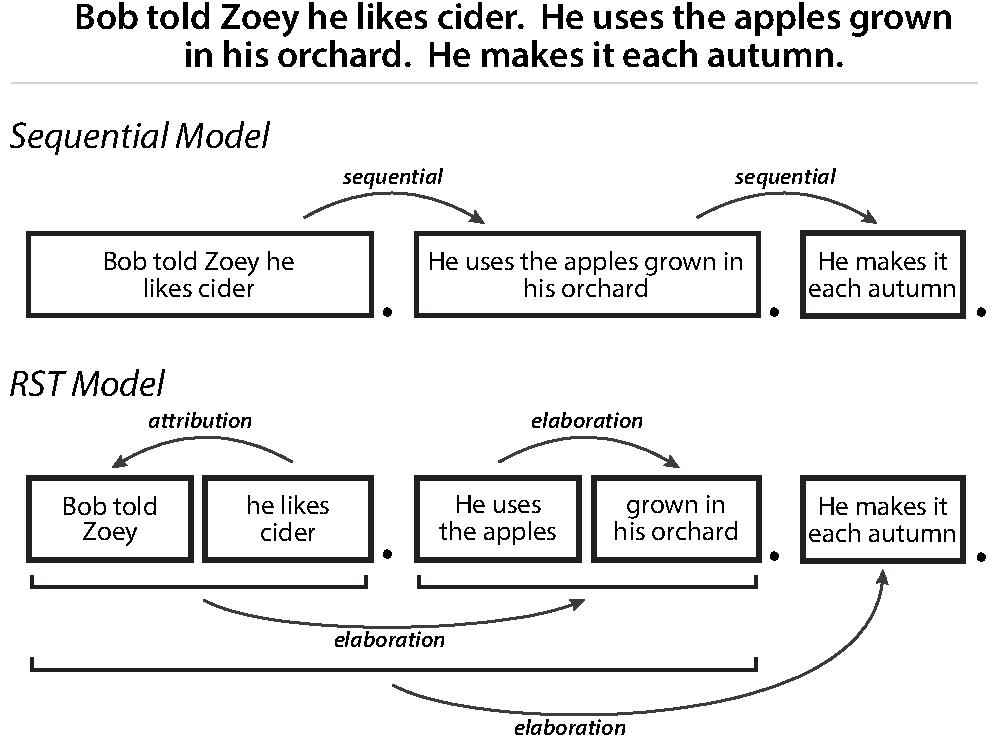
\includegraphics[width=75mm]{rst2a.pdf}
\vspace{-2mm}
\caption{{\small An example of the alignments produced by the two discourse models.  The sequential model aligns pairs of consecutive sentences, capturing intersentence associations such as \emph{cider--apples}, and \emph{orchard--autumn}.  The RST model generates alignment pairs from participants in all (binary) discourse relations, capturing both intrasentence and intersentence alignments, including 
\emph{apples--orchard, cider--apples}, and \emph{cider--autumn}.}}
% ms: I get the point, but there is value in brevity. Plus, maybe we should not use Bob as example :)
%the intersentence alignments above along with intrasentence and multi-sentence alignments, including \emph{Bob--cider, apples--orchard}, and \emph{cider--autumn}.}}
\vspace{-5mm}
\label{fig:examples}
\end{center}
\end{figure}

\vspace{-1mm}
\section{Approach}
\label{sec:approach}
\vspace{-1mm}

A written text is not simply a collection of sentences, but rather a flowing narrative where sentences and sentence elements depend on each other for meaning -- a concept known as cohesion~\cite{halliday2014cohesion}.  
%We make use of this to generate artificial alignment pairs using discourse.  
Here we examine two methods for generating alignment training data from free text that make use of cohesion: a shallow method that uses only intersentence structures, and a deep method that uses both intrasentence and intersentence structures.
We additionally attempt to separate the contribution of discourse from that of alignment in general by comparing these models against a baseline alignment model which aligns sentences at random.

The first model, the sequential discourse model (SEQ), considers that each sentence continues the narrative  of the previous one, and creates artificial question-answer pairs from all pairs of consecutive sentences.
% ms: no space
%This is similar to a right-attachment baseline in dependency parsing, 
%but operating at sentence granularity rather than word.
Thus, this model takes advantage of intersentence cohesion by aligning the content words\footnote{In pilot experiments, we found that aligning only nouns, verbs, adjectives, and adverbs yielded higher performance.} in each sentence with the content words in the following sentence.  For example, in the passage in Figure \ref{fig:examples}, this model would associate \emph{cider} in the first sentence with \emph{apples} and \emph{orchard} in the second sentence.

The second model uses RST to capture discourse cohesion both within and across sentence boundaries.  
We extracted RST discourse structures using an in-house parser~\cite{Surdeanu:15}, which follows the architecture introduced by Hernault et al.~\citeyear{hernault10} and Feng and Hirst~\citeyear{feng12}.
The parser first segments text into elementary discourse units (EDUs), which may be at sub-sentence granularity, then recursively connects neighboring units with binary discourse relations, such as \emph{Elaboration} or \emph{Contrast}.\footnote{The RST parser performs better on relations which occur more frequently.  We use only relations that occurred at least 1\% of the time.  This amounted to six relations: \emph{elaboration}, \emph{attribution}, \emph{background}, \emph{contrast}, \emph{same-unit}, and \emph{joint}. Using all relations slightly improves performance by 0.3\% P@1.} Our parser differs from previous work with respect to feature generation in that we implement all features that rely on syntax using solely dependency syntax. For example, a crucial feature used by the parser is the dominance relations of Soricut and Marcu~\citeyear{soricut2003}, which capture syntactic dominance between discourse units located in the same sentence. While originally these dominance relations were implemented using constituent syntax, we provide an equivalent implementation that relies on dependency syntax. The main advantage to this approach is speed: the resulting parser performs at least an order of magnitude faster than the parser of Feng and Hirst~\citeyear{feng12}. 

Importantly, we generate artificial alignment pairs from this imposed structure by aligning the governing text (nucleus) with its dependent text (satellite).\footnote{Pilot experiments showed that this direction of alignment performed better than aligning from satellite to nucleus.} 
 Turning again to the example in Figure \ref{fig:examples}, this RST-based model captures additional alignments that are both intrasentence, e.g., \emph{apples--orchard}, and intersentence, e.g., {\em cider--autumn}. 
% intersentence associations of the sequential baseline, in addition it finds an intrasentence association between \emph{apples} and \emph{orchard}. 

%\todo{The random alignment baseline (RND) was created in a similar fashion to the SEQ model, except that the sentences were randomly shuffled first.  In the open domain this shuffling took place within a document, and in the biology domain it was done across the entire of the textbook.}



%----------------------TABLE FORMAT FROM TACL 2015--------

\begin{table*}[h]{}

\begin{scriptsize}

        \centering
        %\resizebox{7.9cm}{!}{
        {
        %\begin{tabular}{p{1cm}|p{3cm}|l}
        \begin{tabular}{p{0.3cm}|p{5cm}|p{8cm}}
        \hspace*{-7pt}  & Feature Group & Feature Descriptions \\
        \toprule
        \multirow{10}{*}
        {\rotatebox[origin=c]{90}{~~~~~~~~~Alignment Models}}
        & { Global Alignment Probability } & p(Q$|$A) according to IBM Model 1 \cite{Brown:93}\\ 
        & {} & {}\\
        & { Jenson-Shannon Distance (JSD) } & {Pairwise JSDs were found between the probability distribution of each content word in the question and those in the answer.  The \textbf{mean, minimum, and maximum JSD values} were used as features. Additionally, composite vectors were formed which represented the entire question and the entire answer and the \textbf{overall JSD} between these two vectors was also included as a feature. See Fried et. al \citeyear{fried2015higher} for additional details.} \\
        \midrule
        \multirow{10}{*}
        {\rotatebox[origin=c]{90}{~~~~~~~~~~~~~~~~~~~~~~~~~~~~~~~~~~RNNLM}}
        & { Cosine Similarity } & {Similar to Jansen et al.~\citeyear{jansen14}, we include as features the {\bf maximum and average pairwise cosine similarity} between question and answer words, as well as the {\bf overall similarity} between the composite question and answer vectors.} \\
        \bottomrule
        \end{tabular}
        }
        %}

\end{scriptsize}

        %\caption{$10$ most important features of each sieve.}
        \caption{Feature descriptions for alignment models and RNNLM baseline.}
        \label{tab:Features}
	\vspace{-6mm}

\end{table*}

%------------------END COPIED TABLE----------------
%space{-1mm}
\section{Models and Features}
\label{sec-naacl2015:models}

We evaluate the contribution of these alignment models using a standard reranking architecture~\cite{jansen14}.
The initial ranking of candidate answers is done using a shallow candidate retrieval (CR) component.\footnote{We use the same cosine similarity between question and answer lemmas as Jansen et al.~\citeyear{jansen14}, weighted using {\em tf.idf}.} % (see Ch. 6, \cite{manning08}).}  
Then, these answers are reranked using a more expressive model that incorporates alignment features alongside the CR score.  As a learning framework we use \svmr , a Support Vector Machine tailored for ranking.\footnote{ \url{http://www.cs.cornell.edu/people/tj/svm_light/svm_rank.html}}
We compare this alignment-based reranking model against one that uses a state-of-the-art recurrent neural network language model (RNNLM)~\cite{mikolov10,mikolov13}, which has been successfully applied to QA previously~\cite{yih13}.


%IBM Model 1 \cite{Brown:93} \todo{GIZA++?} was used to generate the discourse pair matrices described in section \ref{sec-naacl2015:approach} for the alignment models.  Each of these models, along with a Recurrent Neural Network Language Model (RNNLM), was used to rerank candidate answers in a shallow retrieval model which used \svmr , a Support vector Machine tailored for ranking.\footnote{ \url{http://www.cs.cornell.edu/people/tj/svm_light/svm_rank.html}}  
%(See Jansen~\citeyear{jansen14} for detailed architecture.\footnote{We also use his \svmr c of 0.1.}) 

{\flushleft {\bf Alignment Model:}}  The alignment matrices were generated with IBM Model 1 \cite{Brown:93} using GIZA++~\cite{och03}, and the corresponding models were implemented as per Surdeanu et al.~\citeyear{Surdeanu:11} with a global alignment probability. 
%, computing a {\bf global alignment probability}, which is the conditional probability of observing a question given an answer.
% ms: the global prob. operates for the whole Q and A!
%question word given an answer word.
%~\footnote{Within Surdeanu et al.'s~\citeyear{Surdeanu:11} framework, we lightly tuned the smoothing parameter, $\lambda$, to 0.4 and we redistributed the probability mass for each word such that the probability of a word translating to itself was 0.5.}  
We extend this alignment model with features from Fried et al.~\citeyear{fried2015higher} that treat each (source) word's probability distribution (over destination words) in the alignment matrix as a distributed semantic representation, and make use the Jensen-Shannon distance (JSD)\footnote{Jensen-Shannon distance is based on Kullback-Liebler divergence but is a distance metric (finite and symmetric).} between these conditional distributions.  A summary of all these features is shown in Table \ref{tab:Features}.% to derive features representing the {\bf minimum, maximum, and average JSDs} between question and answer words, as well as the {\bf overall JSD} between the composite question and answer distributions. 
%Using the Jensen-Shannon distance (JSD) between conditional distributions, content words in each question were compared with the content words in its answers.  Features were made from the maximum, minimum, and average JSDs.  Composite distributions were also created for the entire question and for each entire candidate answer, and the JSD between these composite distributions was used as a feature. 


{\flushleft {\bf RNNLM:}} We learned word embeddings using the \texttt{word2vec} RNNLM of Mikolov et al. \citeyear{mikolov13}, and include the cosine similarity-based features described in Table \ref{tab:Features}. %Similar to Jansen et al.~\citeyear{jansen14}, we include as features the {\bf maximum and average pairwise cosine similarity} between question and answer words, as well as the {\bf overall similarity} between the composite question and answer vectors. 

%{\flushleft {\bf Hyperparameters}}We used the following very lightly tuned hyperparameters: for \svmr, we used c = 0.1 and for IBM model 1, lambda = 0.4 and self-association of 0.5. \todo{re-write this!! or spread to appropriate places} 

\section{Experiments}
\label{sec-naacl2015:experiments}

%\subsection{Data}
%\label{sec-naacl2015:data}
%\vspace{-2mm}


We tested our approach in two different domains, open-domain and cellular biology. For consistency we use the same corpora as Jansen et al.~\citeyear{jansen14}, which are described briefly here. 

{\flushleft {\bf Yahoo! Answers (YA):}}  Ten thousand open-domain \emph{how} questions were randomly chosen from the Yahoo! Answers\footnote{\url{http://answers.yahoo.com}} community question answering corpus and divided: 50\% for training, 25\% for development, and 25\% for test.  Candidate answers for a given question are selected from the corresponding answers proposed by the community (each question has an average of 9 answers).

{\flushleft {\bf Biology QA (Bio):}} 183 \emph{how} and 193 \emph{why}  questions in the cellular biology domain were hand-crafted by a domain expert, and paired with gold answers in the Campbell's Biology textbook~\cite{Reece:2011}.  Each paragraph in the textbook was considered as a candidate answer.  As there were few questions, five fold cross-validation was used with three folds for training, one for development, and one for test.

%In both set-ups, candidate answers were assigned a candidate retrieval (CR) score based on the lexical similarity of the question to the candidate answer.~\footnote{In the Bio task, the CR also incorporated a similarity between the question and the section containing the candidate answer paragraph.}  That CR score served as both a strong baseline for the models (when used alone) as well as an additional feature to be used alongside the model features described in section \ref{sec-naacl2015:models}.
%\subsection{Sources for Alignment}
%\label{sources}

{\flushleft {\bf Alignment Corpora}}: To train the alignment models we generated alignment pairs from two different resources: Annotated Gigaword \cite{Napoles2012} for YA, and the textbook for Bio.  Each was discourse parsed with the RST discourse parser described in Section~\ref{sec-naacl2015:approach}, which is implemented in the FastNLPProcessor toolkit\footnote{\url{http://github.com/sistanlp/processors}}, using the MaltParser\footnote{\url{http://www.maltparser.org/}} for syntactic analysis.
% and reimplements the discourse model of Feng and Hirst~\citeyear{feng12}, using solely features extracted from dependency syntax.


%To explore the relationship between amount of available training data and performance, after each resource was discourse parsed it was divided into samples of exponentially increasing size.  For AGiga, there were 12 sizes ranging from one document to 10,000 and for the textbook, there were 10 sizes ranging from one subsection up to the entire book (2686 subsections).  Additionally, there were 10 samples for each size to reduce the margin of error. 
%condense this---
%To demonstrate the utility of our approach in generating surrogate training data for limited resource domains, we evaluated the performance of our models with incremental amounts of data.  
%{\flushleft {\bf Annotated gigaword \todo{CITE}(AGiga)}}: After discourse parsing AGiga in its entirety, we randomly selected 10 files.  From each we made 12 samples that exponentially increased in size, from 1 document up to 10,000.~\footnote{The larger samples contained the same documents as the smaller samples from the same file so as to represent consistently growing knowledge.}  
%{\flushleft {\bf Campbells}}:For Bio, Campbell's textbook was divided at the subsection level, discarding any subsection consisting of only a single sentence, for a total of 2686 subsections.  These subsections were shuffled to generate 10 random permutations and 10 samples exponentially increasing in number of subsections were made from each.  

\subsection{Results and Discussion}
\label{sec-naacl2015:results}

\begin{figure}[t!]
\begin{center}
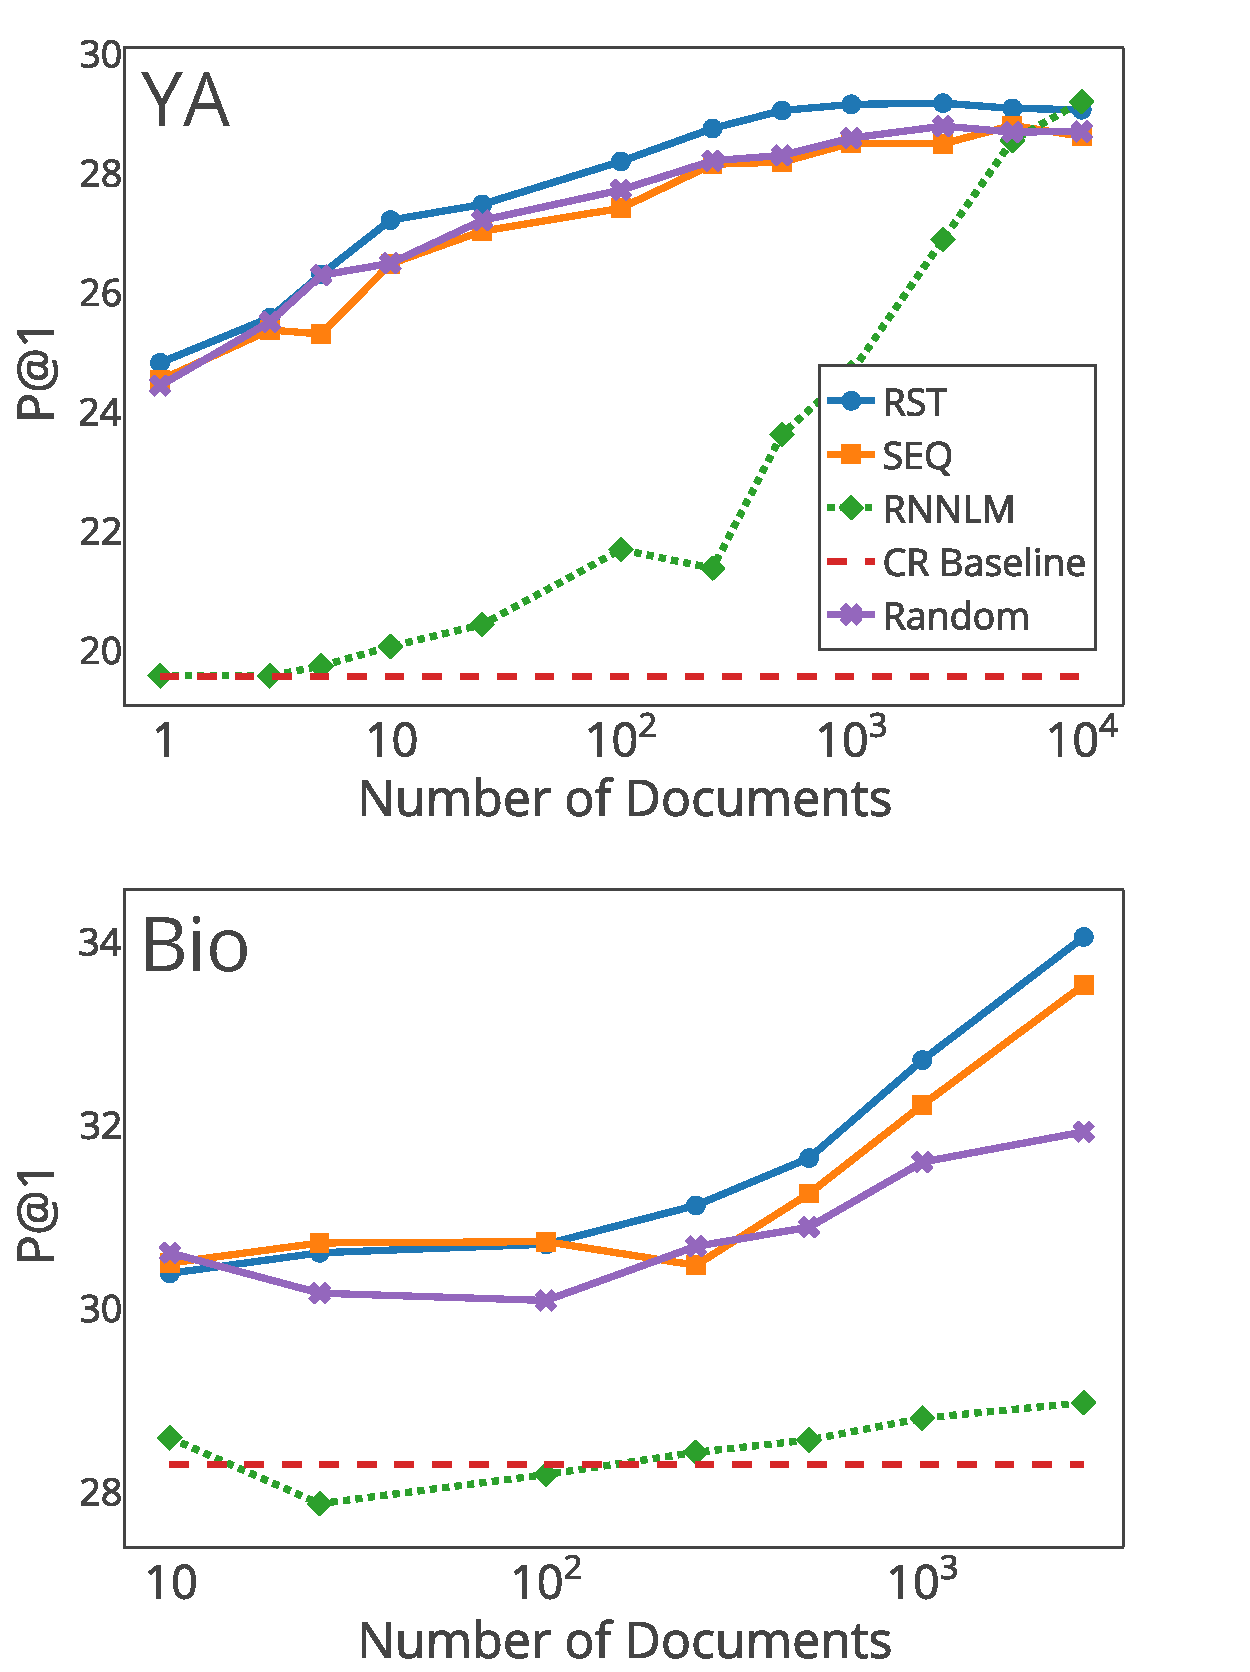
\includegraphics[width=90mm]{mainmatter/naacl2015-alignment/graphs_test2a.pdf}
%\vspace{-4mm}
\caption{{\small Overall performance for the two discourse-based alignment models,
compared against the CR baseline, random baselines, and a RNNLM-based reranker.
%, sequential, and lexical semantic models versus the number of training documents used to construct the models.  
The $x$ axis indicates the number of training documents used to construct all models. 
Each point represents the average of 10 samples of training documents.  }}
%space{-6mm}
\label{fig:performance}
\end{center}
\end{figure}

\begin{comment}
\begin{table}[t!]
\begin{center}
%\begin{scriptsize}
\begin{footnotesize}
\begin{tabular}{llc}
\multicolumn{1}{l}{ } & \multicolumn{1}{l}{ } & \multicolumn{1}{l}{P@1} \\
\multicolumn{1}{l}{ Model/Features } & \multicolumn{1}{l}{P@1} & \multicolumn{1}{l}{Impr.} \\
\cline{2-3}

\hline
\multicolumn{3}{l}{\textit{Yahoo! Answers}} \\ % 185q (sent) ret=1p c=0.1 
\hline
CR Baseline 	& 19.48 	&	  				\\
CR + RST  		& 28.98		& +48.75\% 			\\
CR + SEQ  		& 28.53		& +46.45\% 			\\
CR + RNNLM  		& 29.11		& +49.44\% 			\\
\hline
\multicolumn{3}{l}{\textit{Bio WHY}} \\ % 185q (sent) ret=1p c=0.1 
\hline
CR Baseline 	& 28.24 	&	  				\\
CR + RST  		& 34.00		& +20.38\% 			\\
CR + SEQ  		& 33.47		& +18.53\% 			\\
CR + RNNLM  		& 28.92		& +2.39\% 			\\
\end{tabular}
\end{footnotesize}
\caption{{\small Final performance for the discourse, sequential, and lexical semantic models as compared to the candidate retrieval baseline. For space reasons data for Bio WHY are shown but the pattern is essentially identical for Bio HOW.}}
\label{tab:overall}
\end{center}
\end{table}
\end{comment}
Figure \ref{fig:performance} shows the performance of the discourse models against the number of documents used to train the alignment model.\footnote{For space reasons the graph for Bio \emph{how} is not shown, but the pattern is essentially identical to Bio \emph{why}.}   We used the standard implementation for P@1 ~\cite{manning08} with the adaptations for Bio described in Jansen et al.~\citeyear{jansen14}. We address the following questions.
%, and compare against the CR baseline and RNNLM-based reranker.

\paragraph{How does the performance of the RST and SEQ models compare?}
% and to the baselines?}
Comparing the two principal alignment models, the RST-based model significantly outperforms the SEQ model by about 0.5\% P@1 in both domains (p $<$ 0.001 for Bio and p $<$ 0.01 for YA)\footnote{All reported statistics were performed at the endpoints, i.e., when all training data is used, using bootstrap resampling with 10,000 iterations.}. This shows that deep discourse analysis (as imperfect as it is today) is beneficial. 

\paragraph{How does the performance of the RST model compare to a model trained on in-domain pairs?}

Both the RST and SEQ results for YA are {\em higher} than that of an alignment model trained on explicit in-domain question-answer pairs. Fried et. al \citeyear{fried2015higher} trained an identical alignment model using approximately 65k QA pairs from the YA corpus, and report a performance of 27.24\% P@1, or nearly 2 points lower than our model trained using 10,000 Gigaword documents. This is an encouraging result, which further demonstrates that: (a) discourse analysis can be exploited to generate artificial semi-structured data for alignment, and (b) the sequential model, which also outperforms Fried et. al, can be used as a reasonable proxy for discourse when a parser is not available. 


\paragraph{How does the performance of the RST model compare to previous work?}

Comparing our work to Jansen et al. \citeyear{jansen14}, the most relevant prior work, we notice two trends.
First, our discourse-based alignment models outperform their CR + RNNLM model, which peaks at 26.6\% P@1 for YA and 31.7\% for Bio \emph{why}. While some of this difference can be assigned to implementation differences (e.g., we consider only content words for both alignment and RNNLM, where they used all words), this result again emphasizes the value of our approach.
% Second, while our content-filtered RNNLM outperforms their unfiltered model\footnote{RNNLM performance is slightly less in Bio as we use only the textbook for training.}, when using equal amounts of training data, our alignment model trained using discourse still outperforms the RNNLM until the performance of all models ultimately plateaus in knowledge-rich environments.  
Second, the partially lexicalized discourse structures used by Jansen et. al to identify explanatory text in candidate answers perform better than our approach, which relies solely on lexicalized alignment. However, we expect that our two approaches are complementary, because they address different aspects of the QA task (structure vs. similarity).
%the performance of our alignment models be orthogonal to their discourse models, 
%as we don't explicitly use discourse structures to identify answer candidates in our reranker.

\paragraph{How do the RST and SEQ models compare to the non-alignment baselines?}

%Both the RST and SEQ alignment models \todo{significantly} %considerably 
%outperform the CR and RNNLM baselines, especially for few training documents or domain-specific (Bio) settings.\footnote{The immediate performance boost seen by the alignment models even for 1 training document is explained by the fact the the global alignment probability of Surdeanu et al. (2011) explicitly models word self associations, which complements well the vector space model of the CR baseline.}  

In Bio, both the RST and SEQ alignment models significantly outperform the RNNLM and CR baselines (p $<$ 0.001).  %Additionally, the RST model does significantly better than the SEQ model (p $<$ 0.001).  
In YA, the RST and SEQ models significantly outperform the CR baseline (p $<$ 0.001), and though 
%and the RST model also does significantly better than the RND baseline (p $<$ 0.05) though the SEQ does not (p $>$ 0.1).% as well as the SEQ model (p $<$ 0.01).  
they considerably outperform the the RNNLM baseline for most training document sizes, when all 10,000 documents are used for training, they do not perform  better.  
%Finally, the SEQ model is not significantly better than the RND baseline (p $>$ 0.1).
This shows that alignment models are more robust to little training data, but RNNLMs catch up when considerable data is available.

%RND??
%with both models approaching 34\% P@1 in Bio (or 20\% over the CR baseline), and 29\% P@1 in YA (up to a 49\% relative performance gain over the CR baseline). \textcolor{red}{In YA, when all training documents are used, the performance of the RST model was significantly higher the SEQ model (p $<$ 0.01) as well as all baselines (p $<$ *** for all).  The YA SEQ model performance was not significantly different than that of the RND baseline (p $>$ ***) but was ***.  In Bio...  As the amount of training data in Bio increases, performance gaps of the various models widen.  That is, when enough signal builds up, we can see the increase in efficacy of lexical associations when words go from simply being within the same domain (tRND), to broadly cohesive (SEQ), to finally having a fine-grained discourse connection (RST).}

\paragraph{How does the SEQ model compare to the RND baseline?}
In Bio, the SEQ model significantly outperforms the RND baseline (p $<$ 0.001) but in YA it does not.  This is likely due to differences in the size of the document which was randomized.  In YA, the sentences were randomized within Gigaword articles, which are relatively short (averaging 19 sentences), whereas in Bio the randomization was done at the textbook level.  In practice, as document size decreases, the RND model approaches the SEQ model.


%% Cut for space
%\paragraph{What is the contribution of the individual discourse relations used in generating the alignment pairs?}
%\begin{table}[t!]
%\begin{center}
%\begin{footnotesize}
%\begin{tabular}{llclc}
%\multicolumn{1}{l}{ } & \multicolumn{1}{c}{YA} & \multicolumn{1}{c}{Bio} 		\\
%\multicolumn{1}{l}{ Discourse Relations } & \multicolumn{1}{c}{P@1} & \multicolumn{1}{c}{P@1}		\\
%\cline{2-3}
%\hline
%All  	&  29.23	&	 34.39  \\
%Top 6 (92\% of data)  	& 28.98		& 34.00 	\\
%\end{tabular}
%\end{footnotesize}
%\caption{{Comparison of performance for the discourse model when all discourse relations are used versus when only the top 6 most frequent (\textit{elaboration, attribution, background, contrast, joint, and same-unit}) are used.}}
%\vspace{-6mm}
%\label{tab:ablation}
%\end{center}
%\end{table}
%
%As shown in Table \ref{tab:ablation}, the bulk of the performance comes from using the six most frequent discourse relations (of 18 possible discourse relations).  This is likely due to the fact that these top six relations make up 92\% of all relations in both domains. 



\paragraph{Why does performance plateau in YA and not in Bio?}

With Bio, we exploit all of the limited in-domain training data, and continue to see performance improvements.  With YA, however, performance asymptotes for the alignment models when trained beyond 10,000 documents, or less than 1\% of the Gigaword corpus.  Similarly, when trained over the entirety of Gigaword (two orders of magnitude more data), our RNNLM improves only slightly, peaking at approximately 30.5\% P@1 (or, a little over 1\% P@1 higher).  
We hypothesize that this limitation comes from failing to take context into account. 
%In highly technical domains, such as biology, words like {\em phosphorylation} are non-ambiguous, whereas 
In open domains, alignments such as {\em apple -- \mbox{orchard}} may interfere with those from different contexts, e.g., {\em apple -- computer}, and add noise to the answer selection process.  
%This is empirically supported by the data: in Figure \ref{fig:performance} the steep slope of the Bio corpus shows no signs of decreasing even beyond $10^{3}$ documents, whereas in YA it begins to plateau after $10^{2}$ documents.  This suggests that by incorporating context into alignment models for QA, there is the potential to further capitalize on the remaining training data available. 

%For YA, this is the case until nearly all 10,000 documents are used, at which point the RNNLM finally reaches the performance of the alignment models (RST had 48.75\%, SEQ 46.45\%, and RNNLM 49.44\% P@1 relative over the CR baseline).  
%Not demonstrated with our experimental design, in (hidden for review) the performance of the RNNLM is also shown to plateau around 30\% P@1, even when all of gigaword is used to train the vectors.  
%In the highly technical Bio domain, both the RST and SEQ alignment models far outperform the RNNLM across all sample sizes (20.38\%, 18.53\% and 2.39\% P@1 relative over the CR baseline, respectively).  In both domains, the deep RST model using both intersentence and intrasentence associations outperforms the shallow SEQ model using only intersentence associations.

%In comparison to previous work in Jansen et al \citeyear{jansen14}, for YA our final RNNLM performance is higher due to implementational differences (29.11\% P@1 from 10,000 documents compared to their 26.57\% using all of gigaword).  In Bio, our final RNNLM performance is lower (28.92\% P@1 compared to their 31.73\%) because we trained our RNNLM only on the in-domain textbook, as opposed to the expanded corpus they used.  Both the RST and SEQ models, however, performed better than their RNNLM (34.00\% and 33.47\% P@1 respectively), demonstrating that by using our approach to impose structure for alignment we can attain better results with less data.  Additionally, as we don't explicitly use discourse features, we expect that the performance demonstrated here would be orthogonal to that of their deep and shallow discourse models.

%While performance steadily increases with the size of training data, for both alignment and RNNLM models we asymptote at approximately 30\% P@1 and 10,000 training documents for YA (while we are limited by the available training data for Bio). 







%This is likely due to general alignment model limitations coupled with domain differences between gigaword (a news-domain) and CQA.  As more and more documents are included in training, perhaps the model becomes too far biased towards news to continue to increase performance.  In pilot experiments, we found that using as many as 20 files did not improve performance and in (hidden for review) when all of gigaword is used to train the vectors, the performance of the RNNLM plateaus around the same 30\% P@1. As the data used here is a small fraction of the data available, there is potential for performance increases if more sophisticated techniques, such as topic filtering, are implemented.  

%space{-1mm}
\section{Conclusion}
\label{sec-naacl2015:conclusion}
%space{-2mm}

We propose two inexpensive methods for training alignment models using solely free text, by generating artificial question-answer pairs from discourse structures. 
%Using a RST discourse parser, one method generates both intrasentence and intersentence alignments that can be combined to reach peak performance. For domains where a discourse parser is not available, the second aligns sequential sentences provides a close approximation.  
%Both of these models offer methods for low-resource domains where training data is expensive and/or limited. 
Our experiments indicate that these methods are a viable solution for constructing state-of-the-art QA systems for low-resource domains, or languages where training data is expensive and/or limited.  Since alignment models have shown utility in other tasks (e.g. textual entailment), we hypothesize that these methods for creating inexpensive and highly specialized training data could be useful for tasks other than QA.  

%% Cut for space
%Our generation tool, {\tt Straw2Gold}, is available at: {\small \url{http://nlp.sista.arizona.edu/releases/straw2gold}}.

%Future work should be done to determine the extent of immediate application as well as ways to refine the methods for these other uses.


%By imposing structure over free text,  monolingual alignment can used to achieve large performance gains in non-factoid QA.  When discourse parsing is practical for the domain in question, both intrasentence and intersentence alignments can be combined to reach peak performance, and for domains where this isn't possible, aligning sequential sentences provides a close approximation.  Both of these models offer methods for low-resource domains where training data is expensive and/or limited. 

%---------------------------------------DISCUSSION

%In fact, it is notable how quickly we see performance increases from the alignment models in YA.  In both domains, results are increased due to word self-associations (when the same word appears in both the question and the answer), but with YA there also is a slight correlation between answer length and correctness.  The magnitude of the performance increase due to these factors is essentially shown in the results for the smallest sample size, as one document doesn't contain enough data to provide a real alignment contribution.  
%Taking this into account, the scores still increase quite rapidly for YA.  It could be the case that associations between high frequency verbs drive much of this performance.  If so, then perhaps for the more technical Bio domain, more world-knowledge (encoded in nouns and other parts of speech) is needed,  explaining why we don't see the same immediate performance gain.  To test this, matrices could be made with only verbs, only nouns, or other combinations to determine if one type of association is driving much of the performance and how the domains compare in this respect. 

%After a rapid increase, the performance in YA quickly levels off relative to the amount of input for training.~\footnote{Only a fraction of 1 file is used to achieve the maximal performance for the alignment models.  In pilot experiments, including as many as 20 files did not improve performance. }  This may be a result of a decrease in the signal to noise ratio.  Unlike YA, gigaword is within the news domain.  As more and mode documents are added to training, perhaps the model becomes too far biased towards news to continue to increase performance.  If more sophisticated techniques are implemented, such as topic filtering, potentially the performance in this domain could be even higher.  We don't see the same plateau effect with Bio that we do with YA.  Likely this is due to the fact that the in-domain texbook for Bio was much smaller than gigaword.  

%\todo{strong close}
%---------------------------------------OLD
%when all 10,000 documents are used for training, the models have similar performance.  The asymptotic behavior of the RST and SEQ models is rendered in Figure \ref{fig:performance} and in (hidden for review) the RNNLM is also shown to plateau around 30\% P@1 even when all of gigaword is used to train the vectors.~\footnote{Only a fraction of one file is used to achieve this performance plateau for the alignment models.  In pilot experiments we found that including up to 20 files does not improve performance though it does drastically affect runtime.}.  When fewer documents are used, however, the gap in performance is substantial.  
%Additionally, though not demonstrated with our experimental design, rather than surpass the alignment model performance the RNNLM has been shown to plateau around 30\% P@1 even when all of gigaword is used to train the vectors (hidden for review).    

%In the YA task, with all 10,000 documents the average performance for the RST model was 28.98\% , for the SEQ model it was 28.53(48.75\% and 46.45\% relative over the CR baseline respectively~\footnote{Only a fraction of 1 file is used to achieve this performance plateau for the alignment models and including up to 20 \emph{files} does not improve performance though it does drastically affect runtime. }.  While the RNNLM reaches the peak results of the alignment models when all 10,000 documents are used (49.44\% relative over CR baseline), when fewer are available the gap in performance is substantial.  \todo{p-values for everything}.  Additionally, though not demonstrated with our experimental design, rather than surpass the alignment model performance the RNNLM has been shown to plateau around 30\% P@1 even when all of gigaword is used to train the vectors (hidden for review).  

%\section{Discussion}
\label{sec-cl2017:discussion}

To further characterize the performance of our QA approach, we address the following questions: 


%%
%% Comparison with TableILP
%%
%\begin{table}[t]
%\caption{{ Comparison with other models }} % 
%\small
%\begin{center}
%\begin{tabular}{lccc}
%%\cline{2-3}
%%\begin{tabular}{p{20mm}cc}
%\hline
%\multicolumn{1}{c}{Model} & \multicolumn{1}{c}{Questions} &\multicolumn{1}{c}{P@1} \\
%\cline{2-3}
%\hline
%CR $\cup$ (1G\textsubscript{CT} + 2G\textsubscript{CT}) $\cup$ 3G\textsubscript{CT} 			 	& 1000		&	44.6\%	\\
%Khashabi et. al (2016)																				& 200 		&	45.6\%	\\
%
%\end{tabular}
%\label{tab:tableilp}
%\end{center}
%\end{table}

{\flushleft {\bf How does performance compare with methods using manually constructed knowledge bases?}} The TAG system automatically aggregates sentences from six free-text corpora first by building graphlets from those sentences using syntactic dependencies, then connecting those graphlets together into multisentence text aggregation graphs that are then used to both answer questions and provide a compelling human-readable justification for the selected answers.  Recently, Khashabi et al. \citeyear{Khashabi2016QuestionAV} demonstrated that graphs for elementary science QA can also be constructed using a semistructured knowledge base of tables.  In this formalism, dozens of themed tables are manually or semi-automatically constructed, each around a particular theme.  A table's theme is encoded in it's columns, i.e., a table for the color of objects contains two rows, one for the object of interest (e.g., ``leaf''), and another for it's color (e.g., ``green''), while separate instances (e.g., leaf -- green, trunk -- brown) are encoded as different rows.  Each table has between two and five columns.  

The TableILP algorithm answers questions by chaining facts between different table rows, starting from a row that contains question terms, then traversing to a new table row that contains some lexical overlap with the previous row(s), until answer terms are found.  The TAG and TableILP systems are conceptually similar, with the central differences being: (1) The TableILP table row is roughly equivalent to a TAG graphlet with flat structure, and limited to 2--5 information nuggets containing only single terms, (2) TAG graphlets are read automatically from free text corpora, where TableILP tables are largely manually constructed, with methods to automate this construction being actively developed, and (3) the traversal algorithms are different, with TableILP graph building being modelled as an integer linear programming (ILP) problem which finds paths that maximize QA performance.  

The TableILP system reported by Khashabi et al. \citeyear{Khashabi2016QuestionAV} contains 69 tables containing a total of 7,600 rows, with 64 of these tables (approximately 5,000 rows) designed around material in the study guides and a development corpus, and the remaining 2,600 rows distributed amoung 4 automatically constructed tables.  On a corpus of 200 questions drawn from the 1,000 questions used here, TableILP achieved a score of 45.6\% P@1\footnote{We wish to thank Khashabi et al. \citeyear{Khashabi2016QuestionAV} for providing us with this performance figure.}, compared to the 44.6\% P@1 from the best-performing TAG model in Table~\ref{tab:combinedmodels}. The performance difference between these systems is likely not statistically significant.\footnote{We did not have access to system output. However, in our experiments on this dataset, we observed that only differences in P@1 scores of 3\% or higher (absolute) tend to be statistically significant at $p < 0.05$.}

We view these systems as complementary, converging, and with each capable of exploring different aspects of graph-based inference for science QA.  While the TAG focuses on automatically building graphs from free text, this is currently a challenging and noisy process, and as we have shown in Table~\ref{tab:pathlength} and Fried et al.~\citeyear{fried2015higher}, highly susceptable to inference drift as the amount of information required to be aggregated becomes large.  On the other hand, building graphs from manually constructed knowledge bases allow us to investigate the graph-building process in isolation, reducing inference drift due to noise, and further moving this area forward.  

%
% Performance by grade level
%
\begin{table}[t]
\caption{{ Precision@1 by grade level. }} % 
\small
\begin{center}
\begin{tabular}{lccc}
%\cline{2-3}
%\begin{tabular}{p{20mm}cc}
\hline
\multicolumn{1}{c}{Grade Level} & \multicolumn{1}{c}{Questions} &\multicolumn{1}{c}{CR} & \multicolumn{1}{c}{TAG}  \\
\cline{2-3}
\hline
Grade 3 	& 60		&	28.3\%		& 49.2\%	\\
Grade 4		& 69 	&	50.7\%		& 41.3\%	\\
Grade 5		& 871	&	40.2\%		& 42.6\%	\\

\end{tabular}
\label{tab:gradelevel}
\end{center}
\end{table}


{\flushleft {\bf How does performance vary by grade level?}} The question corpus contains third, fourth, and fifth grade questions.  A human with a level of knowledge equivalent to a fourth grade science student might be expected to show better performance for the simpler third grade questions, and decreasing performance as question difficulty increases from fourth to fifth grades.  Table~\ref{tab:gradelevel} shows P@1 performance by grade level for both the CR and best performing TAG model (1G\textsubscript{CT} + 2G\textsubscript{CT}).  The TAG model shows decreasing performance as question difficulty increases, dropping from 49\% for third grade questions to 42\% for fourth and fifth grade questions.  The CR baseline, however, displays a qualitatively different pattern, with a peak performance of 51\% for fourth grade questions, and {\em near chance} performance for third grade questions. 
We believe that observing such a pattern in performance may suggest that the TAG model is a closer approximation of human inference than the baseline based solely on information retrieval.  Here, the relatively small number of third and fourth grade questions prevents us from drawing any conclusions, but suggests that crafting question sets to allow evaluating the distribution of performance by grade level may provide a further measure of comparison between human and machine performance. 



%
% Justification performance by knowledge resource
%
\begin{table}[t]
\caption{{ Most useful knowledge resources for justifications classified as "good".}}
\small
\begin{center}
\begin{tabular}{lccc}
%\cline{2-3}
%\begin{tabular}{p{20mm}cc}
\hline
\multicolumn{1}{l}{Resource} & \multicolumn{1}{c}{Sentences} &\multicolumn{1}{c}{CR} & \multicolumn{1}{c}{TAG}  \\
\cline{2-3}
\hline
Barrons SG 			& 1,200		&	39.3\%		& 43.0\%	\\
Flashcards			& 283		&	16.2\%		& 8.2\%	\\
Teacher's Guide		& 302		&	7.1\%		& 7.0\%	\\
Virginia SG			& 1,314		&	9.1\%		& 9.2\%	\\
Science Dictionary	& 733		&	20.8\%		& 17.8\%	\\
Simple Wiktionary	& 17,473		&	7.5\%		& 14.8\%	\\

\end{tabular}

\label{tab:justificationknowledgeresources}
\end{center}
\end{table}

{\flushleft {\bf Which knowledge resources are generating the most useful answer justifications?}} Shown in Table~\ref{tab:justificationknowledgeresources}, the Barron's Study Guide (SG) contributes more of the \emph{good} justification sentences than any other source, followed by the science dictionary, then the other resources.  Interestingly, the Simple Wicktionary contributes the fewest sentences to the \emph{good} justifications for the CR system (7.5\%), but for the TAG system it is the third largest contributor (14.8\%).  That is, while the CR system is typically unable to find a \emph{good} justification from the Wiktionary, likely owing to it's general nature, the TAG system is able to successfully aggregate these sentences with sentences from other domain-specific sources to build complete justifications.

The vast majority of the \emph{good} justifications generated by the TAG system are aggregates from non-adjacent text: 67\% of the justifications aggregate sentences from \emph{different} corpora, 30\% aggregate non-adjacent sentences within a \emph{single} corpus, while only 3\% of \emph{good} justifications contain sentences that were adjacent in their original corpus. 
This is clear evidence that information aggregation (or fusion) is fundamental for answer justification.


{\flushleft {\bf How orthogonal is the performance of the TAG model when compared to CR?}} Both the TAG and CR models use the same knowledge resources, which on the surface suggests the models may be similar, answering many of the same questions correctly.  The voting models in Table~\ref{tab:combinedmodels} appear to support this, where combining the TAG and CR models increases performance by just under 2\% P@1 over the best-performing TAG model.  To investigate this, we conducted an orthogonality analysis to determine the number of questions both models answer correctly, and the number of questions each model uniquely answers correctly.

Comparing the TAG (1G\textsubscript{CT} + 2G\textsubscript{CT}) and CR models, nearly half of questions are answered correctly by one model and incorrectly by the other.  When combined into a two-way voting model, this causes a large number of ties -- which, resolved at chance, would perform at 42\%, with ceiling performance (i.e., all ties resolved correctly) at 60\%.  This indicates that while the TAG and CR models share about half of their performance, each model is sensitive to different kinds of questions, suggesting that further combination strategies between TAG and CR are worth exploring.


%\section{Discussion}
\label{sec-cl2017:discussion}

To further characterize the performance of our QA approach, we address the following questions: 


%%
%% Comparison with TableILP
%%
%\begin{table}[t]
%\caption{{ Comparison with other models }} % 
%\small
%\begin{center}
%\begin{tabular}{lccc}
%%\cline{2-3}
%%\begin{tabular}{p{20mm}cc}
%\hline
%\multicolumn{1}{c}{Model} & \multicolumn{1}{c}{Questions} &\multicolumn{1}{c}{P@1} \\
%\cline{2-3}
%\hline
%CR $\cup$ (1G\textsubscript{CT} + 2G\textsubscript{CT}) $\cup$ 3G\textsubscript{CT} 			 	& 1000		&	44.6\%	\\
%Khashabi et. al (2016)																				& 200 		&	45.6\%	\\
%
%\end{tabular}
%\label{tab:tableilp}
%\end{center}
%\end{table}

{\flushleft {\bf How does performance compare with methods using manually constructed knowledge bases?}} The TAG system automatically aggregates sentences from six free-text corpora first by building graphlets from those sentences using syntactic dependencies, then connecting those graphlets together into multisentence text aggregation graphs that are then used to both answer questions and provide a compelling human-readable justification for the selected answers.  Recently, Khashabi et al. \citeyear{Khashabi2016QuestionAV} demonstrated that graphs for elementary science QA can also be constructed using a semistructured knowledge base of tables.  In this formalism, dozens of themed tables are manually or semi-automatically constructed, each around a particular theme.  A table's theme is encoded in it's columns, i.e., a table for the color of objects contains two rows, one for the object of interest (e.g., ``leaf''), and another for it's color (e.g., ``green''), while separate instances (e.g., leaf -- green, trunk -- brown) are encoded as different rows.  Each table has between two and five columns.  

The TableILP algorithm answers questions by chaining facts between different table rows, starting from a row that contains question terms, then traversing to a new table row that contains some lexical overlap with the previous row(s), until answer terms are found.  The TAG and TableILP systems are conceptually similar, with the central differences being: (1) The TableILP table row is roughly equivalent to a TAG graphlet with flat structure, and limited to 2--5 information nuggets containing only single terms, (2) TAG graphlets are read automatically from free text corpora, where TableILP tables are largely manually constructed, with methods to automate this construction being actively developed, and (3) the traversal algorithms are different, with TableILP graph building being modelled as an integer linear programming (ILP) problem which finds paths that maximize QA performance.  

The TableILP system reported by Khashabi et al. \citeyear{Khashabi2016QuestionAV} contains 69 tables containing a total of 7,600 rows, with 64 of these tables (approximately 5,000 rows) designed around material in the study guides and a development corpus, and the remaining 2,600 rows distributed amoung 4 automatically constructed tables.  On a corpus of 200 questions drawn from the 1,000 questions used here, TableILP achieved a score of 45.6\% P@1\footnote{We wish to thank Khashabi et al. \citeyear{Khashabi2016QuestionAV} for providing us with this performance figure.}, compared to the 44.6\% P@1 from the best-performing TAG model in Table~\ref{tab:combinedmodels}. The performance difference between these systems is likely not statistically significant.\footnote{We did not have access to system output. However, in our experiments on this dataset, we observed that only differences in P@1 scores of 3\% or higher (absolute) tend to be statistically significant at $p < 0.05$.}

We view these systems as complementary, converging, and with each capable of exploring different aspects of graph-based inference for science QA.  While the TAG focuses on automatically building graphs from free text, this is currently a challenging and noisy process, and as we have shown in Table~\ref{tab:pathlength} and Fried et al.~\citeyear{fried2015higher}, highly susceptable to inference drift as the amount of information required to be aggregated becomes large.  On the other hand, building graphs from manually constructed knowledge bases allow us to investigate the graph-building process in isolation, reducing inference drift due to noise, and further moving this area forward.  

%
% Performance by grade level
%
\begin{table}[t]
\caption{{ Precision@1 by grade level. }} % 
\small
\begin{center}
\begin{tabular}{lccc}
%\cline{2-3}
%\begin{tabular}{p{20mm}cc}
\hline
\multicolumn{1}{c}{Grade Level} & \multicolumn{1}{c}{Questions} &\multicolumn{1}{c}{CR} & \multicolumn{1}{c}{TAG}  \\
\cline{2-3}
\hline
Grade 3 	& 60		&	28.3\%		& 49.2\%	\\
Grade 4		& 69 	&	50.7\%		& 41.3\%	\\
Grade 5		& 871	&	40.2\%		& 42.6\%	\\

\end{tabular}
\label{tab:gradelevel}
\end{center}
\end{table}


{\flushleft {\bf How does performance vary by grade level?}} The question corpus contains third, fourth, and fifth grade questions.  A human with a level of knowledge equivalent to a fourth grade science student might be expected to show better performance for the simpler third grade questions, and decreasing performance as question difficulty increases from fourth to fifth grades.  Table~\ref{tab:gradelevel} shows P@1 performance by grade level for both the CR and best performing TAG model (1G\textsubscript{CT} + 2G\textsubscript{CT}).  The TAG model shows decreasing performance as question difficulty increases, dropping from 49\% for third grade questions to 42\% for fourth and fifth grade questions.  The CR baseline, however, displays a qualitatively different pattern, with a peak performance of 51\% for fourth grade questions, and {\em near chance} performance for third grade questions. 
We believe that observing such a pattern in performance may suggest that the TAG model is a closer approximation of human inference than the baseline based solely on information retrieval.  Here, the relatively small number of third and fourth grade questions prevents us from drawing any conclusions, but suggests that crafting question sets to allow evaluating the distribution of performance by grade level may provide a further measure of comparison between human and machine performance. 



%
% Justification performance by knowledge resource
%
\begin{table}[t]
\caption{{ Most useful knowledge resources for justifications classified as "good".}}
\small
\begin{center}
\begin{tabular}{lccc}
%\cline{2-3}
%\begin{tabular}{p{20mm}cc}
\hline
\multicolumn{1}{l}{Resource} & \multicolumn{1}{c}{Sentences} &\multicolumn{1}{c}{CR} & \multicolumn{1}{c}{TAG}  \\
\cline{2-3}
\hline
Barrons SG 			& 1,200		&	39.3\%		& 43.0\%	\\
Flashcards			& 283		&	16.2\%		& 8.2\%	\\
Teacher's Guide		& 302		&	7.1\%		& 7.0\%	\\
Virginia SG			& 1,314		&	9.1\%		& 9.2\%	\\
Science Dictionary	& 733		&	20.8\%		& 17.8\%	\\
Simple Wiktionary	& 17,473		&	7.5\%		& 14.8\%	\\

\end{tabular}

\label{tab:justificationknowledgeresources}
\end{center}
\end{table}

{\flushleft {\bf Which knowledge resources are generating the most useful answer justifications?}} Shown in Table~\ref{tab:justificationknowledgeresources}, the Barron's Study Guide (SG) contributes more of the \emph{good} justification sentences than any other source, followed by the science dictionary, then the other resources.  Interestingly, the Simple Wicktionary contributes the fewest sentences to the \emph{good} justifications for the CR system (7.5\%), but for the TAG system it is the third largest contributor (14.8\%).  That is, while the CR system is typically unable to find a \emph{good} justification from the Wiktionary, likely owing to it's general nature, the TAG system is able to successfully aggregate these sentences with sentences from other domain-specific sources to build complete justifications.

The vast majority of the \emph{good} justifications generated by the TAG system are aggregates from non-adjacent text: 67\% of the justifications aggregate sentences from \emph{different} corpora, 30\% aggregate non-adjacent sentences within a \emph{single} corpus, while only 3\% of \emph{good} justifications contain sentences that were adjacent in their original corpus. 
This is clear evidence that information aggregation (or fusion) is fundamental for answer justification.


{\flushleft {\bf How orthogonal is the performance of the TAG model when compared to CR?}} Both the TAG and CR models use the same knowledge resources, which on the surface suggests the models may be similar, answering many of the same questions correctly.  The voting models in Table~\ref{tab:combinedmodels} appear to support this, where combining the TAG and CR models increases performance by just under 2\% P@1 over the best-performing TAG model.  To investigate this, we conducted an orthogonality analysis to determine the number of questions both models answer correctly, and the number of questions each model uniquely answers correctly.

Comparing the TAG (1G\textsubscript{CT} + 2G\textsubscript{CT}) and CR models, nearly half of questions are answered correctly by one model and incorrectly by the other.  When combined into a two-way voting model, this causes a large number of ties -- which, resolved at chance, would perform at 42\%, with ceiling performance (i.e., all ties resolved correctly) at 60\%.  This indicates that while the TAG and CR models share about half of their performance, each model is sensitive to different kinds of questions, suggesting that further combination strategies between TAG and CR are worth exploring.



%space{-2mm}
%\begin{small}
\section*{Acknowledgments}
%space{-2mm}
We thank the Allen Institute for AI for funding this work.
%\end{small}

%\bibliographystyle{acl}
%\bibliography{citations} % add your references to citations, then run bibtex

% If you use BibTeX with a bib file named eacl2014.bib, 
% you should add the following two lines:
%\bibliographystyle{acl}
%\bibliography{acl2014}
%\bibliography{refs}
%\bibliography{citations}



%\twocolumn[\centering \Large \bf Creating Causal Embeddings for Question Answering \\with Minimal Supervision \par
%~\\
%
%\large \bf Anonymous EMNLP submission
%~\\
%~\\
%]

%\begin{abstract}
%A common model for question answering (QA) is that a good answer is one that is closely related to the question, where relatedness is often determined using general-purpose lexical models such as word embeddings. 
%We argue that a better approach is to look for answers that are related to the question in a {\em relevant way}, according to the information need of the question,
%%We argue that a better approach is to look for answers that are related to the question in {\em the right way} \todo{"the right way" doesn't say much... Can we say something like "in a way relevant to the type of information need, or something like that?}, 
%which may be determined through task-specific embeddings. 
%With causality as a use case, we implement this insight in three steps. First, we generate causal embeddings cost-effectively by bootstrapping cause-effect pairs extracted from free text using a small set of seed patterns. Second, we train dedicated embeddings over this data, by using task-specific contexts, i.e., the context of a cause is its effect. Finally, we extend a state-of-the-art reranking approach for QA to incorporate these causal embeddings. We evaluate the causal embedding models both \emph{directly} with a casual implication task,
%% \todo{"Word similarity" makes it sound like we do lexical similarity... Can you say something causal implication?}, 
% and \emph{indirectly}, in a downstream causal QA task using data from Yahoo! Answers. We show that explicitly modeling causality improves performance in both tasks. In the QA task our best model achieves 37.3\% P@1, significantly outperforming a strong baseline by 7.7\% (relative). 
%% ms: not sure if we should discuss the differences between the 2 tasks here; we might not have space; it might dilute the message.
%
%%
%%Question answering (QA) is a difficult task, complicated by the variety of question types represented in any given question set.  In this work we propose addressing question types individually through the use of dedicated relation embeddings, and here focus on causal relations. 
%%We train causal embeddings (as well as two other popular distributional similarity models) on causal tuples extracted from free text resources with minimal supervision, using a small set of high-precision patterns.   
%%We evaluate these causal models both \emph{directly} in terms of their ability to detect causality, and \emph{indirectly}, in terms of their utility on a causal subset of Yahoo! Answers.
%%In both tasks, we show that explicitly modeling causality significantly improves performance, and in the QA task our best model achieves 37.3\% precision at one, outperforming a strong information retrieval and lexical semantic baseline by 7.7\% (relative). 
%%Importantly, we also show that the results of these two evaluations are \emph{not} identical: a given model's performance on the direct evaluation does not necessarily transfer to the more complex, real-world QA task.  
%\end{abstract}

\chapter{EMNLP2016 - CAUSAL EMBEDDINGS\label{chapter:emnlp2016}}



%
\section{Introduction}
\label{sec-emnlp2016:introduction}
%\vspace{-2mm}

Question answering (QA), i.e., finding short answers to natural language questions, is one of the most important but challenging 
tasks on the road towards natural language understanding~\cite{Etzioni:11}. 
A common approach for QA is to prefer answers that are closely related to the question, where relatedness is often determined using lexical semantic models such as word embeddings~\cite{yih13,jansen14,fried2015higher}. 
%Many QA systems answer questions by looking for answers that are closely related to the question, often as determined with lexical semantic word embeddings~\todo{citation}.  
While appealing for its robustness to natural language variation, this one-size-fits-all approach does not take into account the wide range of distinct question types that can appear in any given question set, and that are best addressed individually~\cite{chu2004ibm,ferrucci2010building,clark2013study}.  

Given the variety of question types, we suggest that a better approach is to look for answers % which are not simply closely related to the question, 
that are related to the question \emph{through the appropriate relation}, e.g., a causal question should have a cause-effect relation with its answer.
If we adopt this view, and continue to work with embeddings as a mechanism for assessing relationship,
this raises a key question: how do we train and use task-specific embeddings cost-effectively? 
Using causality as a use case, we answer this question with a framework for producing causal word embeddings with minimal supervision, and a demonstration that such task-specific embeddings significantly benefit causal QA. 
%Adopting this view, here we propose using task-specific word embeddings that combine the robustness and versatility of word embeddings with the precision of addressing a specific question type.  
%As a use case, we focus on producing custom embeddings with minimal supervision that capture causality and that are thus directly applicable to causal QA.

%\todo{REMOVE?: One important hurdle for QA is that there isn't a single ``universal engine'' that can answer any question, but rather a collection of methods, each tailored to a specific question type (e.g., factoid, definitional, or causal).
%This has been repeatedly observed throughout QA research, in various domains
%\cite{chu2004ibm,ferrucci2010building,clark2013study}. 
%Building from this observation, this paper proposes a framework for developing specific QA solving methods, and, in particular, on the rapid bootstrapping of knowledge resources needed by these solving methods. We encode this knowledge as customized embedding vectors, and demonstrate that they can be generated with minimal supervision. As a use case, we focus on producing custom embeddings that capture \textit{causality} and that are thus directly applicable to causal QA. }

In particular, the contributions of this work are:

%{\flushleft {\bf (1)}} 
%A novel approach for question answering that uses task-specific distributional similarity models 

{\flushleft {\bf (1)}} 
A methodology for generating causal embeddings cost-effectively by bootstrapping cause-effect pairs extracted from free text using a small set of seed patterns, e.g., {\em X causes Y}. 
%We propose a method to generate knowledge resources for causal questions 
%We demonstrate that knowledge resources for causal questions can be generated by bootstrapping cause-effect pairs extracted from free text using a small set of high-precision patterns, e.g., {\em X causes Y}. 
We then train dedicated embedding (as well as two other distributional similarity) models over this data. \citet{levy2014dependency} have modified the algorithm of\citet{mikolov2013distributed} to use an arbitrary, rather than linear, context. Here we make this context task-specific, i.e., the context of a cause is its effect.
%embedding models (as well as alignment and convolutional neural network models) over this data. 
Further, to mitigate sparsity and noise, our models are bidirectional, and noise aware (by incorporating the likelihood of noise in the training process). 
%We achieve the latter by weighting the examples based on the likelihood that they are truly causal rather than simply associative. 

{\flushleft {\bf (2)}} The insight that QA benefits from task-specific embeddings. % , and a demonstration that this approach significantly improves performance. 
We implement a QA system that uses the above causal embeddings to answer questions and demonstrate that they significantly improve performance over a strong baseline. Further, we show that causal embeddings encode complementary information to vanilla embeddings, even when trained from the same knowledge resources. 

{\flushleft {\bf (3)}} An analysis of direct vs. indirect evaluations for task-specific word embeddings. 
We evaluate our causal models both  {\em directly}, in terms of measuring their capacity to rank causally-related word pairs over word pairs of other relations, as well as {\em indirectly} in the downstream causal QA task. 
%Importantly, the above knowledge acquisition process is completely independent from these evaluation tasks, e.g., the objective function of the embedding model does not include any information from the QA task, which guarantees modularity. 
In both tasks, our analysis indicates that including causal models significantly improves performance. 
However, from the direct evaluation, it is difficult to estimate which models will perform best in real-world tasks. Our analysis re-enforces recent observations about the limitations of word similarity evaluations~\cite{faruqui2016problems}: we show that they have limited coverage and may align poorly with real-world tasks.

%{\flushleft {\bf (3)}} For causal QA, we show that causal embeddings encode complementary information to vanilla embeddings, even when trained from the same knowledge resources. 

%the models that include causal embeddings perform significantly better than the models that do not. Further, for causal QA, we show that causal embeddings are complementary to vanilla embeddings, underlining the complexity of this QA task, which must simultaneously capture causality and associations driven by distributional similarity. \todo{reword? seems like we're contradicting our earlier statement...}

%{\flushleft {\bf (4)}} Finally, we show that there are discrepancies between direct and indirect evaluations, i.e., no model performs best in both tasks. Our analysis re-enforces recent observations about the limitations of narrow word similarity evaluations~\cite{faruqui2016problems}, in that they both have limited coverage, and can poorly align with real world tasks.

%
\section{Related Work}
\label{sec-emnlp2016:related work}
%\vspace{-2mm}

%QA with dedicated component
Addressing the need for %In the pursuit of %quest for building 
specialized solving methods in QA, 
Oh et. al~\citeyear{oh2013question} incorporate a dedicated causal component into their system, and note that it improves the overall performance.  However, their model is limited by the need for lexical overlap between a causal construction found in their knowledge base and the question itself.  Here, we develop a causal QA component that exploits specialized word embeddings to gain robustness to lexical variation.  
%which can model the likelihood of a causal link between two texts even when the exact lexical items were never observed together in the knowledge base.

% Embeddings in QA
There has been a vast body of work which demonstrates that word embeddings derived from distributional similarity are useful in many tasks, including question answering -- see \emph{inter alia}~\mbox{\cite{fried2015higher,yih13}}.  However, Levy and Goldberg~\citeyear{levy2015supervised} note that there are limitations on the type of semantic knowledge which is encoded in these general-purpose similarity embeddings. 
Therefore, here we build customized task-specific embeddings for causal QA.

%% Customized embeddings
Customized embeddings have been created for a variety of tasks, including semantic role labeling~\cite{fitzgerald2015semantic,woodsenddistributed}, and binary relation extraction ~\mbox{\cite{riedel2013relation}.}
%% For example, with semantic role labelling, custom embeddings have been learned for semantic frames, their arguments, and the roles of the arguments (e.g. \cite{fitzgerald2015semantic,woodsenddistributed}).  Riedel et al.~\citeyear{riedel2013relation} used distant supervision to learn embeddings for binary relations and argument pairs to perform automated database completion.  
%Like Riedel et al., we are interested in binary relations, but we train a dedicated embedding space for a single such relation, while they represent all relations in a single embeddding space.
Similar to Riedel et al., we train embeddings customized for specific relations, but we bootstrap training data using minimal supervision (i.e., a small set of patterns) rather than relying on distant supervision and large existing knowledge bases.  Additionally, while Riedel et al. represent all relations in a general embedding space, here we train a dedicated embedding space for just the causal relations. 
%\todo{remove: this is just text so that my citation doesn't fall across page boundaries, which makes latex cry}

In QA, embeddings have been customized to have question words that are close to either their answer words~\cite{bordes2014question}, or to structured knowledge base entries~\cite{yang2014joint}.  While these methods are useful for QA, they do not distinguish between different types of questions, and as such their embeddings are not specific to a given question type.

Additionally, embeddings have been customized to distinguish functional similarity from relatedness ~\cite{levy2014dependency,kielaspecializing}.
In particular, Levy and Goldberg train their embeddings by replacing the standard linear context of the target word with context derived from the syntactic dependency graph of the sentence.  For example, when given the word \emph{turing}, wheras a traditional embeddings model returns top associates containing topically related words such as \emph{non-deterministic} and \emph{finite-state}, the dependency-based model returns other tests (i.e., \emph{pauling, hotelling,} and \emph{hamming}).
In this work, we make use of this extension to arbitrary context in order to train our embeddings with contexts derived from binary causal relations.  We extract cause-effect text pairs such that the cause text becomes the \emph{target} text and the effect text serves as the \emph{context}. 

Recently, Faruqui et al.\citeyear{faruqui2016problems} discussed issues surrounding the evaluation of similarity word embeddings, including the lack of correlation between their performance on word-similarity tasks and ``downstream'' or real-world tasks like QA, text classification, etc.  As they advocate, in addition to a direct evaluation of our causal embeddings, we also evaluate them independently in a downstream QA task.  We provide the same comparison for two alternative approaches (an alignment model and a convolutional neural network model), confirming that the direct evaluation performance can be misleading without the task-specific, downstream evaluation. 

%\todo{better intro target/context} In this way, words which \emph{cause similar things} would be top-associates of each other.  

%In the search for ways to represent the semantic information encoded in words and text, there have been several methods proposed which are based on the distributional hypothesis of \todo{cite}.  The distributional hypothesis asserts that words which are semantically similar will tend to occur in similar word contexts.  One of the methods based on this hypothesis, the Skipgram algorithm \todo{cite and link}, or \texttt{word2vec}\footnote{\todo{link!}}, has been widely used for far-ranging NLP tasks.  This algorithm maps words onto high-dimensional dense vectors (embeddings) in such a way that words which are more similar to each other are closer together in the high-dimensional space.%, often measured through cosine similarity.  

%Levy and Goldberg also suggest that the traditional skipgram vectors encode broad topical similarity, and propose an extension of the algorithm which replaces the linear context of a given target word with arbitrary context.  
%While there we make use of the same  rather than topical similarity.  For example, when given the word \emph{turing}, wheras the traditional skipgram model returns top associates containing topically related words such as \emph{non-deterministic} and \emph{finite-state}, the dependency-based model returns other tests (i.e., \emph{pauling, hotelling,} and \emph{hamming}).

%While the specific implementation of Levy and Goldberg~\citeyear{levy2014dependency} uses dependency-derived contexts for training, their extension of the algorithm allows for \emph{arbitraty} contexts.  
%Additionally, though seldom used, the skipgram algorithm produces two sets of embeddings for each word, one for when the word serves as a target word and another for when the word serves as a context word.  Here, since the relation of interest is inherently directional, both sets of embeddings are meaningful, and so we make use of both -- the target vectors when a given word appears as a cause and the context vectors when that word appears as an effect.




%--Causal Patterns
With respect to extracting causal relations from text, Girju et al.~\citeyear{girju2002text} use modified Hearst patterns~\cite{hearst1992automatic} to extract a large number of potential cause-effect tuples, where both causes and effects must be nouns.
However, Cole et al.~\citeyear{cole2005lightweight} show that these nominal-based causal relations account for a relatively small percentage of all causal relations, and for this reason, \cite{yang2014multi} allow for more elaborate argument structures in their causal extraction by identifying verbs, and then following the syntactic subtree of the verbal arguments to construct their candidate causes and effects. 
Additionally, Do et al.~\citeyear{do2011minimally} observe that nouns as well as verbs can signal causality.  
We follow these intuitions in developing our causal patterns by using both nouns and verbs to signal potential participants in causal relations, and then allowing for the entire dominated structures to serve as the cause and/or effect arguments.

%Khoo did this over newspapers too


%\todo{POSSIBLY MOVE TO METHODS: 
%Khoo et al.~\citeyear{khoo1998automatic} also extract causal tuples using linguistic patterns, and in their error analysis they find that the majority of their errors of commission (i.e., %mislabelling a construction as casual) result from lexical ambiguity.  That is, several lexical constructions which can signal causality are also used in non-causal senses.  To minimize the noise %in the extracted pairs, we restrict ourselves to patterns with low ambiguity. 
%Further, inspired by bootstrapping literature~\cite{riloff1996automatically}, we rank the extracted tuples by their likelihood of being noisy using a formula driven by mutual information, and %adjust the training process of the embedding models to use this information.
%}


\section{Specialized question answering}
%\label{sec:related_work_emnlp2016}

A common model for question answering (QA) is that a good answer is one that is closely related to the question, where relatedness is often determined using general-purpose lexical models such as word embeddings. 
Here we argue that a better approach is to look for answers that are related to the question in a {\em relevant way}, according to the information need of the question (that is, the question type).
In this way, a QA system might consist of many distinct solvers, each specialized to the inference needs of a particular question type, such as causal inference or reasoning over a process\footnote{Not addressed here is \textit{how} questions are to be classified, and it is very much open-ended. Not only is the \textit{number} of classes open-ended, but also the \textit{type} of the classes themselves -- for example you could base them on domain (e.g., Biology versus Geology, etc.), or, as discussed here the inference type required (e.g., causal versus definitional, etc.), or some other dimension entirely.  Even after determining a classification scheme, developing the classifier itself is certainly non-trivial, made more difficult by the fact that complex questions can potentially belong to several different classes, as described by \citet{jansen-EtAl:2016:COLING}.  However, this is beyond the scope of the current work.}.  Here we explore one framework that could be used for these solvers, which we use to answer causal questions.  We argue that this general framework can be extended easily to handle other question types.

We are not the first to assert the need for specialized solving methods in QA.  For example, \citet{oh2013question} incorporate a dedicated causal component into their system, and note that it improves the overall performance.  However, their model is limited by the need for explicit lexical overlap between a causal construction found in their knowledge base and the question itself.  Here, we develop a causal QA component that exploits specialized word embeddings that are task-specific (i.e., specifically learned to model the desired semantic relation, here \textit{causality}), to gain robustness to lexical variation.  
By using word embeddings, we can model the likelihood of a causal link between two texts even when the exact lexical items were never observed together in the knowledge base.

\subsection{Embeddings for question answering}
% Embeddings in QA
There has been a vast body of work which demonstrates that word embeddings derived from distributional similarity are useful in many tasks, including question answering~\mbox{\citep[see \emph{inter alia}][]{fried2015higher,yih13}}.  However, \citet{levy2015supervised} note that there are limitations on the type of semantic knowledge which is encoded in these general-purpose similarity embeddings.  Therefore, rather than limit ourselves to the general purpose embeddings, here we build task-specific embeddings that are customized for answering causal questions.

\subsection{Customizing embeddings}
%% Customized embeddings
Customized embeddings have been created for a variety of tasks. %including semantic role labeling~\citep{fitzgerald2015semantic,woodsenddistributed}, and binary relation extraction ~\mbox{\citep{riedel2013relation}.}
For example, with semantic role labelling, custom embeddings have been learned for semantic frames, their arguments, and the roles of the arguments~\citep[e.g.,][]{fitzgerald2015semantic,woodsenddistributed}.  \citet{riedel2013relation} used distant supervision to learn embeddings for binary relations (such as \textit{employed\_by}) and argument pairs (such as $<$\textit{Jane Smith, Harvard}$>$) in order to perform automated database completion.  
Similar to \citeauthor{riedel2013relation}, we train embeddings customized for specific relations, but we bootstrap training data using minimal supervision (i.e., a small set of patterns) rather than relying on distant supervision and large existing knowledge bases.  Additionally, while Riedel et al. represent \textit{all} relations in a general embedding space, here we train a dedicated embedding space for just the causal relations. 

For use in question answering, embeddings have been customized to have question words that are close to either their answer words~\citep{bordes2014question}, or to structured knowledge base entries~\citep{yang2014joint}.  While these methods are useful for QA, they do not distinguish between different types of questions, and as such their embeddings are not specific to a given question type.

Additionally, embeddings have been customized to distinguish functional similarity from relatedness ~\citep{levy2014dependency,kielaspecializing}.
In particular, Levy and Goldberg train their embeddings by replacing the standard linear context of the target word with context derived from the syntactic dependency graph of the sentence.  The resulting embeddings, they argue, model functional similarity rather than topical similarity.  For example, when given the word \emph{turing}, wheras a traditional embeddings model returns top associates containing topically related words such as \emph{non-deterministic} and \emph{finite-state}, the dependency-based model returns other tests (i.e., \emph{pauling, hotelling,} and \emph{hamming}).
In this work, we make use of this extension to arbitrary context in order to train our embeddings with contexts derived from binary causal relations.  We extract cause-effect text pairs such that the cause text becomes the \emph{target} text and the effect text serves as the \emph{context}. This raises the issue of multiword target and context texts, which we address in Section \ref{sec-emnlp2016:models}.

Recently, \citet{faruqui2016problems} discussed issues surrounding the evaluation of similarity word embeddings, including the lack of correlation between their performance on word-similarity tasks and ``downstream'' or real-world tasks like QA, text classification, etc.  As they advocate, in addition to a direct evaluation of our causal embeddings (see Section \ref{sec-emnlp2016:directeval}), we also evaluate them independently in a downstream QA task (Section \ref{sec-emnlp2016:indirecteval}).  We provide the same comparison for two alternative approaches (an alignment model and a convolutional neural network model), confirming that the direct evaluation performance can be misleading without the task-specific, downstream evaluation.

\subsection{Chapter overview}

The rest of the Chapter is organized as follows.  
%In Section \ref{sec-emnlp2016:approach} we outline our approach to generating and using causal embeddings for question answering.  
In Section \ref{sec-emnlp2016:causalextraction} we provide details concerning our semi-supervised methods for gathering a large number of cause-effect text pairs that we use for training our models.  In Section \ref{sec-emnlp2016:models} we describe our primary causal embedding models as well as several other variants.  In Section \ref{sec-emnlp2016:directeval} we evaulate these models directly on a causal-relation identification task.  Then, in Section \ref{sec-emnlp2016:indirecteval} we detail the experimental setup for our indirect evaluation: causal QA over a subset of Yahoo! Answers.  We show that explicitly modeling causality improves performance in both the direct and the indirect tasks. In the QA task our best model achieves 37.3\% P@1, significantly outperforming a strong baseline by 7.7\% (relative).
We also show that the results of these two evaluations are \emph{not} identical: a given model's performance on the direct evaluation does not necessarily transfer to the more complex, real-world QA task, as discussed in our conclusions in Section \ref{sec-emnlp2016:conclusion}.


%\begin{figure}[t!]
%\begin{center}
%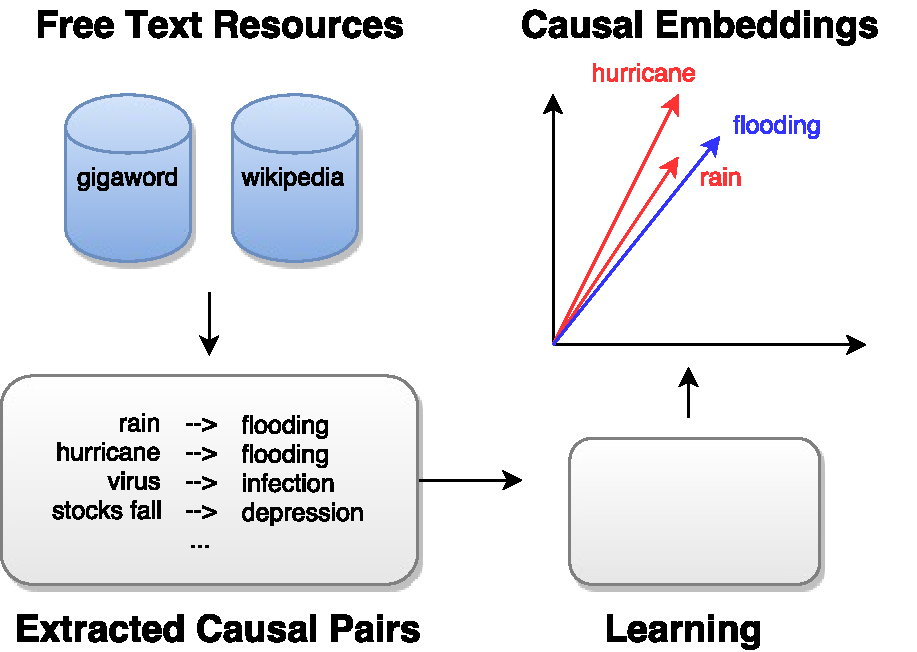
\includegraphics[width=75mm]{emnlpArchDraft.pdf}
%%\vspace{-4mm}
%\caption{{\small Our proposed pipeline for training a causal embedding space from free text resources. \todo{fill in learning with final model}}}
%\vspace{-6mm}
%\label{fig:arch}
%\end{center}
%\end{figure}
%
%\section{Approach}
%\label{sec-emnlp2016:approach}
%%\vspace{-2mm}
%
%Our focus is on reranking answers to causal questions using using task-specific distributional similarity methods.
%%on the the task of question answering, which is complicated by the variety of question types (e.g., definitional, causal),  each having different information needs that potentially require dedicated solving methods~\cite{clark2013study}.  
%%Longer term, we propose a QA approach which uses dedicated, task-specific word embeddings for each question type, aimed at maintaining the robustness of word embeddings while gaining the specificity of dedicated solving methods. 
%%Here, we address one particular information need: causality.
%%
%Our approach operates in three steps:
%
%{\flushleft (1)} We start by bootstrapping a large number of cause-effect pairs from free text using a small number of syntactic and surface patterns (Section \ref{sec-emnlp2016:causalextraction}).
%
%{\flushleft (2)} We then use these bootstrapped pairs to build several task-specific embedding (and other distributional similarity) models (Section \ref{sec-emnlp2016:models}). We evaluate these models directly on a causal-relation identification task (Section \ref{sec-emnlp2016:directeval}).  
%
%{\flushleft (3)} Finally, we incorporate these models into a reranking framework for causal QA and demonstrate that the resulting approach performs better than the reranker without these task-specific models, even if trained on the same data (Section ~\ref{sec-emnlp2016:indirecteval}).  


%We approach the task of creating and evaluating a task-specific relational vector space by considering one relation in particular -- causality.  The architecture of our system is shown in Figure \ref{fig:arch}. \todo{do I really need an architecture here?}

%rule-based framework which analyzes free text and returns cause-effect tuples.  
%These pairs are then used to learn a set of high-dimensional word embeddings which are particular to the desired relation.  
%In particular, we make use of the Levy and Goldberg extension of the skipgram algorithm to learn embeddings from these pairs by predicting the effect-text given the cause-text.
%MOVE:
%using the extension of the Skipgram algorithm~\todo{cite and link} proposed by \citep{levy2014dependency}.  
%\todo{does this belong here? intro?}
%While the learning algorithm returns two distinct vector space embeddings for each item in the vocabulary, often only the target embeddings are ever used.  In this work, however, we make use of both sets of embeddings to capture the inherent \emph{directionality} of the causal relation.

%\todo{remove the evaluation info from here?}
%Once trained, we then evaluate the quality this mapping, or vector space, in two ways.  First, we evaluate it directly by attempting to rank a set of cause-effect pairs higher than entity pairs from other relations.  Second, we evaluate the mapping indirectly, by using it in the down-stream task of question answering (QA).



\section{Extracting Cause-Effect Tuples}
\label{sec-emnlp2016:causalextraction}
%\vspace{-2mm}

%Information extraction (IE) systems which are designed to extract events typically make use of either machine learning (ML) or hand-built rules or patterns.  %IE classifiers which use ML are generally considered to be either fully supervised (trained only on annotated data), semi-supervised (trained on a combination of labelled data and the data which is bootstrapped from it or by using a large database of pre-known event tuples), or unsupervised (when no labelled data is available for training).
%For causal events, we have neither labelled data nor an existing, large database of cause-effect pairs from which we could use ML to train a supervised or semi-supervised classifier.  Additionally, while unsupervised or distant supervision approaches are well-suited to situations where the desired event types and the patterns that would identify them are unknown, here we know exactly what relation we want (causality) and the patterns needed to find these events are relatively explicit.  For these reasons, we opted to use boostrapping to extract a large number of cause-effect pairs from a small set of patterns.

Because the success of embedding models depends on large training datasets \citep{sharp-EtAl:2015:NAACL-HLT}, and such datasets do not exist for open-domain causality, we opted to bootstrap a large number of cause-effect pairs from a small set of patterns.
%
We wrote these patterns using Odin~\citep{valenzuela2016runes}, a rule-based information extraction framework which has the distinct advantage of 
%being able to operate over multiple representations of content (i.e., surface and syntax).
being \emph{expressive}.  That is, while most open-source rule languages operate over one representation of text (e.g., GATE~\citep{Cunningham2011a} generally operates over surface sequences, whereas Semgrex~\citep{chambers2007learning} operates over syntactic dependencies), Odin has the flexibility to use either (or both) depending on the user's need.  
For this work, we make use of rules that operate over both surface sequences as well as dependency syntax in the grammars introduced in steps (2) and (3) below.

Odin operates as a cascade, % of grammars, 
allowing us to implement a two-stage approach.
%. Taking advantage of this architecture, we implemented a two-stage approach.
First, we identify potential participants in causal relations, i.e., the potential causes and effects, which we term {\bf causal mentions}. A second grammar then identifies actual causal relations that take these causal mentions as arguments.

We consider both noun phrases (NP) as well as entire %non-causal
clauses to be potential causal mentions, since causal patterns form around participants that are syntactically more complex than flat NPs.  
%For example, in the sentence \emph{The hurricane caused significant damage}, both the cause ({\em hurricane}) and effect ({\em damage}) are non-recursive noun phrases.  On the other hand, 
For example, in the sentence \emph{The collapse of the housing bubble caused stock prices to fall}, both the cause ({\em the collapse of the housing bubble}) and effect ({\em stock prices to fall}) are more complicated nested structures.  Reducing these arguments to non-recursive NPs (e.g., {\em The collapse} and {\em stock prices}) is clearly insufficient to capture the relevant context.

Formally, we extract our causal relations using the following algorithm:
{\flushleft \textbf{(1) Pre-processing:}} Much of the text we use to extract causal relation tuples comes from the Annotated Gigaword \citep{napoles2012annotated}.  This text is already fully annotated and no further processing is necessary.  We additionally use text from the Simple English Wikipedia\footnote{{\scriptsize \url{https://simple.wikipedia.org/wiki/Main_Page}}.  The Simple English version was preferred over the full version due to its simpler sentence structures, which make extracting cause-effect tuples more straightforward.}, which we processed using the Stanford CoreNLP toolkit~\citep{Manning:14} and the dependency parser of \citet{chen14}.

{\flushleft \textbf{(2) Causal mention identification:}} \label{step:cm} We extract causal mentions (which are able to serve as arguments, i.e., the cause or effect,  in our causal patterns) using a set of rules (shown in Appendix \ref{appendix:cm_rules})\todo{rule appendix!} 
designed to be robust to the variety that exists in natural language. %, and therefore in the dependency parses.  
Namely, to find causal mentions that are noun phrases, we first find words that are tagged as nouns, then follow outgoing dependency links for modifiers and attached prepositional phrases\footnote{The outgoing dependency links from the nouns which we followed were: \texttt{nn, amod, advmod, ccmod, dobj, prep\_of, prep\_with, prep\_for, prep\_into, prep\_on, prep\_to}, and \texttt{prep\_in}.}, to a maximum depth of two links.  To find causal mentions that are clauses, we first find words that are tagged as verbs (excluding verbs which themselves were considered to signal causation\footnote{The verbs we excluded were: \emph{cause, result, lead, create}.}), then again follow outgoing dependency links for modifiers and arguments.  We used a total of four rules to label causal mentions.%\footnote{The two complete grammars, for both causal mention and causal relation identification, were submitted as supplemental material. \todo{This is no longer relevant. Please remove.}}
%There were a total of four rules used to label causal mentions, and examples are shown in Table~\ref{tab:rules}.

{\flushleft \textbf{(3) Causal tuple extraction:}} \label{step:causalext} After causal mentions are identified, a grammar scans the text for causal relations that have causal mentions as arguments.  Different patterns have varying probabilities of signaling causation~\citep{khoo1998automatic}.  To minimize the noise in the extracted pairs, we restrict ourselves to a set of 13 rules designed to find unambiguously causal patterns, such as {\em CAUSE led to EFFECT}, where {\em CAUSE} and {\em EFFECT} are previously found causal mentions.
The rules operate by looking for a \emph{trigger} phrase, e.g., {\em led}, and then following the dependency paths to and/or from the trigger phrase to see if all required causal mention arguments exist.
%, which tells the rule to fire.  Once a trigger is found, the rule follows the dependency paths to and/or from the trigger phrase to see if all specified arguments exist, e.g.,  following an outgoing {\tt nsubj} to identify the cause in the previous example.
%An example of this is shown in Figure \ref{fig:rule_ex}. Here, when the rule scans the sentence \emph{SENTENCE TEXT}, the trigger verb \emph{cause} is found, then the rule checks for an outgoing \texttt{nsubj} dependency link and an outgoing \texttt{dobj} link to previously found causal mentions.  
%%Our grammars also ensure that the triggers are not negated (we used Odin lookaround assertions to check that outgoing \texttt{neg} dependencies are not attached to triggers).  % Since in this example, all conditions are met, the rule returns the causal event in the form of the tuple (\todo{example}).

% ms: removed for space
At step~2, the identification of causal mentions, we place few restrictions on the causal mention syntactic subgraph, favoring recall since in step 3 we use high-precision rules.  The rule set for step \ref{step:causalext}, in fact, was winnowed down after early experiments showed that many patterns which \emph{can} indicate causation (e.g., {\em X happened due to Y}) often are non-causal.  

\begin{table}[t!]
\begin{center}
%\begin{scriptsize}
%\begin{footnotesize}
\begin{tabular}{lc}
\hline
Corpus		&	Extracted Tuples		 \\
\hline
%\multicolumn{2}{l}{\textit{Yahoo! Answers}} \\ % 185q (sent) ret=1p c=0.1 
%\hline
Annotated Gigaword	& 798,808 	\\
Simple English Wikipedia		& 16,425 	\\
\hline
Total		& 815,233 	\\
\end{tabular}
%\end{footnotesize}
\caption{{\footnotesize Number of causal tuples extracted from each corpus.}} 
\label{tab:causalstats}
%space{-4mm}
\end{center}
\end{table}

%ltw_mar30_combo.argsC: 55882
%nyt_mar30_combo.argsC: 260460
%wpb_mar30_combo.argsC: 7522
%apw_mar30_combo.argsC: 219348
%xin_mar30_combo.argsC: 76183
%simpleWiki_mar19b_combo.argsC: 14057
%cna_mar30_combo.argsC: 7913
%afp_mar30_combo.argsC: 133003
%sum: 774368

Applying this causal grammar over Gigaword and Simple English Wikipedia produced 815,233 causal tuples, as summarized in Table~\ref{tab:causalstats}. As bootstrapping methods are typically noisy, we manually evaluated the quality of approximately 250 of these pairs selected at random.  Of the tuples evaluated, approximately 44\% contained some amount of noise. For example, from the sentence 
\begin{quote}
\emph{Except for Springer's show, which still relies heavily on confrontational topics that lead to fistfights virtually every day...}
\end{quote}
%\emph{Except for Springer's show, which still relies heavily on confrontational topics that lead to fistfights virtually every day...}
while ideally we would only extract (\emph{confrontational topics $\rightarrow$ fistfights}), instead we extract the tuple (\emph{show which still relies heavily on confrontational topics} $\rightarrow$ \emph{fistfights virtually every day}), which contains a large amount of noise: \emph{show, relies, heavily}, etc.
This finding prompted our noise-aware model described at the end of Section~\ref{sec-emnlp2016:models}.


\section{Models}
\label{sec-emnlp2016:models}

We use the extracted causal tuples to train three distinct distributional similarity models that explicitly capture causality. 

{\flushleft \textbf{Causal Embedding Model (cEmbed):}}
The first distributional similarity model we use is based on the skip-gram word-embedding algorithm of Mikolov et al.~\citeyear{mikolov2013distributed}, which has been shown to improve a variety of language processing tasks % \footnote{Chris Manning recently called embedding models the Sriracha sauce of NLP.} 
including QA~\cite{yih13,fried2015higher}.  In particular, we use the variant implemented by Levy and Goldberg~\citeyear{levy2014dependency} which modifies the original algorithm to use an arbitrary, rather than linear, context. 
Our novel contribution is to make this context task-specific: intuitively, the context of a cause is its effect. Further, these contexts are generated from tuples that are themselves bootstrapped, which minimizes the amount of supervision necessary.

The Levy and Goldberg model trains using single-word pairs, while our CMs could be composed of multiple words.  
For this reason, we decompose each cause--effect tuple, $(CM_c,CM_e)$, such that each word $w_c \in CM_c$ is paired with each word $w_e \in CM_e$. 

%so we decompose each cause--effect tuple, $(CM_c,CM_e)$, where each CM could be multi-word, into the Cartesian product of the words in CMs. such that each $w_c \in CM_c$ has as its context all $w_e \in CM_e$. 
After filtering the extracted cause-effect tuples for stop words and retaining only nouns, verbs, and adjectives, we generated over 3.6M $(w_c, w_e)$ word-pairs\footnote{For all models proposed in this section we used lemmas rather than words.} from the approximately 800K causal tuples.

The model learns two embedding vectors for each word, one for when the word serves as a target word and another for when the word serves as a context word.  Here, since the relation of interest is inherently directional, both sets of embeddings are meaningful, and so we make use of both -- the target vectors encode the effects of given causes, whereas the context vectors capture the causes of the corresponding effects. 


{\flushleft \textbf{Causal Alignment Model (cAlign):}}
Monolingual alignment (or translation) models have been shown to be successful in QA \cite{Berger:00,Echihabi:03,Soricut:06,Riezler:etal:2007,Surdeanu:11,yao2013}, and recent work has shown that they can be successfully trained with less data than embedding models~\cite{sharp2015spinning}. 
% Further, Fried et al.~\citeyear{fried2015higher} demonstrated that \todo{dest. distribution as semantic model of the source concept, which is important for our task as well.} % ms: nice, but no space

To verify these observations in our context, we train an alignment model that ``translates'' causes (i.e., the ``source language'') into effects (i.e., the ``destination language''), using our cause--effect tuples. 
This is done using IBM Model 1~\cite{Brown:93} and GIZA++~\cite{och03}. 
%We train an alignment model from our cause--effect tuples using  IBM Model 1~\cite{Brown:93} and GIZA++~\cite{och03}.


\begin{figure}[t!]
\begin{center}
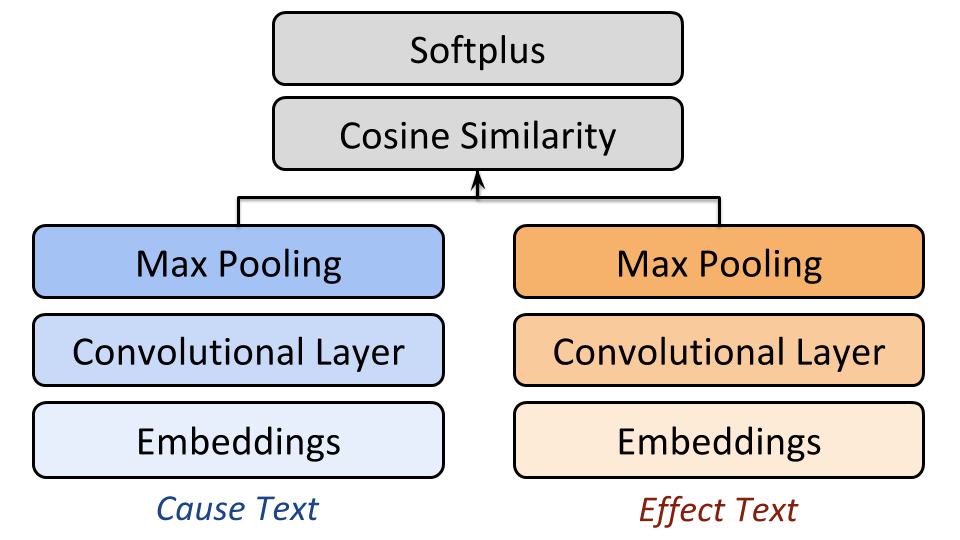
\includegraphics[width=0.7\textwidth]{mainmatter/emnlp2016-causal/cnn2.png}
%space{-2mm}
\caption{{\footnotesize Architecture of the causal convolutional network. }}
%space{-6mm}
\label{fig:cnn}
\end{center}
\end{figure}

{\flushleft \textbf{Causal Convolutional Neural Network Model (cCNN):}}
Each of the previous models have at their root a bag-of-words representation, which is a simplification of the causality task. To address this potential limitation, we additionally trained a convolutional neural network (CNN) which operates over variable-length texts, and maintains distinct embeddings for causes and effects.  The architecture of this approach is shown in Figure~\ref{fig:cnn}, and consists of two sub-networks (one for cause text and one for effect text), each of which begins by converting the corresponding text 
% (which has been padded to be of equal  length)  % ms: skip for now, until we understand it better
into 50-dimensional embeddings.  These are then fed to a convolutional layer,\footnote{The convolutional layer contained 100 filters, had a filter length of 2 (i.e., capturing bigram information), and an inner ReLU activation.} which is followed by a max-pooling layer of equal length.
Then, these top sub-network layers, which can be thought of as a type of phrasal embedding, are merged by taking their cosine similarity.  Finally, this cosine similarity is normalized by feeding it into a dense layer with a single node which has a softplus activation.  
In designing our CNN, we attempted to minimize architectural and hyperparameter tuning by taking inspiration from Iyyer et al.~\citeyear{iyyer2015deep}, preferring simpler architectures.
We train the network using a binary cross entropy objective function and the Adam optimizer~\cite{kingma2014adam}, using the Keras library~\cite{chollet2015keras} operating over Theano~\cite{2016arXiv160502688short}, a popular deep-learning framework.\footnote{We also experimented with an equivalent architecture where the sub-networks are implemented using long short-term memory (LSTM) networks~\cite{hochreiter1997long}, and found that they consistently under-perform this CNN architecture. Our conjecture is that CNNs perform better because LSTMs are more sensitive to overall word order than CNNs, which capture only local contexts, and we have relatively little training data, which prevents the LSTMs from generalizing well.}

{\flushleft \textbf{Noise-aware Causal Embedding Model (cEmbedNoise):}} 
We designed a variant of our cEmbed approach to address the potential impact of the noise introduced by our bootstrapping method.
While training, we weigh the causal tuples by the likelihood that they are truly causal, which we approximate with pointwise mutual information (PMI).
For this, we first score the tuples by their causal PMI and then scale these scores by the overall frequency of the tuple~\cite{riloff1996automatically}, to account for the PMI bias toward low-frequency items.  That is, the score $S$ of a tuple, $t$, is computed as: 

%space{-2mm}
%\scalebox{1.0}{
\begin{small}
\begin{equation}
S(t) = \log \frac{p(tuple|causal)}{p(tuple)} * \log (freq(tuple))
\end{equation} 
\end{small}
%}
%space{-2mm}

%Riloff~\citeyear{riloff1996automatically} propose a method for ranking their extracted patterns using $relevance\_rate * \log_2 (frequency)$.  As our relevance rate we use the pointwise mutual information of the extracted tuples, or $\log \frac{p(tuple|causal)}{p(tuple)}$, where $p(tuple| causal)$ is the ratio of the number of times that a given tuple is found in a causal construction versus any construction, and $p(tuple)$ is the frequency of the given tuple divided by the frequency of all the tuples. 
%Scaling the PMI by the frequency of the tuple mitigates its bias towards low-frequency items.
%we combine PMI with frequency information, so that we consider the likelihood of a pair to be causal to be:
%$p(causal|pair)$ \cite{riloff1996automatically}.
We then discretize these scores into five quantiles, ascribing a linearly decreasing weight during training to datums in lower scoring quantiles.%\footnote{\textcolor{blue}{We implemented this weighing process by repeating higher weight training examples more times.}}



\section{Direct Evaluation: Ranking Word Pairs}

\begin{figure*}[th!]
\begin{center}
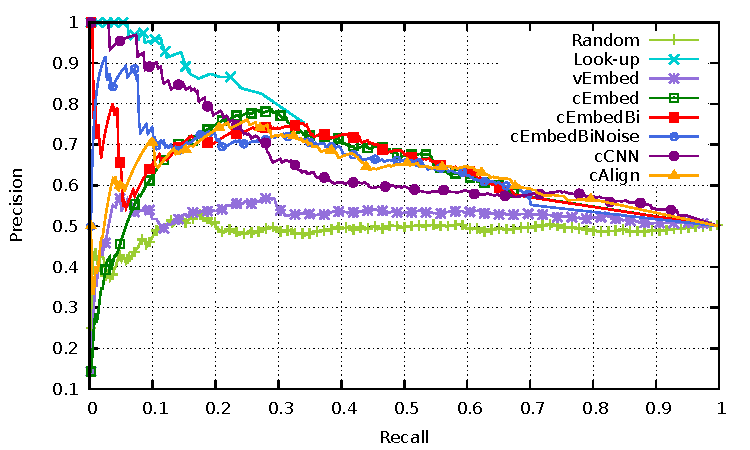
\includegraphics[width=\textwidth]{mainmatter/emnlp2016-causal/direct2.pdf} % {rpcurves_all.png}
%space{-3mm}
\caption{{\footnotesize Precision-recall curve showing the ability of each model to rank causal pairs above non-causal pairs. For clarity, we do not plot cEmbedNoise, which performs worse than cEmbedBiNoise. The Look-up model has no data points beyond the 35\% recall point.}}
%space{-4mm}
\label{fig:rpcurve_all}
\end{center}
\end{figure*}

%\flushleft{\textbf{Results:}} 

\label{sec-emnlp2016:directeval}

%Before we discuss the utility of these models for causal QA, we implement a {\em direct} evaluation
We begin the assessment of our models with a {\em direct} evaluation to determine whether or not the proposed approaches capture causality better than general-purpose word embeddings and whether their robustness improves upon a simple database look-up.
For this evaluation, we follow the protocol of Levy and Goldberg~\citeyear{levy2014dependency}.  
In particular, we create a collection of word pairs, half of which are causally related, with the other half consisting of other relations. 
These pairs are then ranked by our models and several baselines, with the goal of ranking the causal pairs above the others. 
The embedding models rank the pairs using the cosine similarity between the target vector for the causal word and the context vector of the effect word.  The alignment model ranks pairs using the probability $P(\text{Effect}|\text{Cause})$ given by IBM Model 1, and the CNN ranks pairs by the value of the output returned by the network.
%To demonstrate that their embeddings encoded functional similarity rather than relatedness, they ranked a set of word pairs (each of which reflected one of the two types of similarity) using cosine similarity and showed that the word pairs which were functionally similar tended to be ranked higher than those with topical similarity.  Here, we do the same.

%\flushleft{\textbf{Data:}} 
\subsection{Data}
In order to avoid bias towards our extraction methods, we evaluate our models on an external set of word pairs drawn from the SemEval 2010 Task 8 \cite{hendrickx2009semeval}, originally a multi-way classification of semantic relations between nominals.  We used a total of 1730 nominal pairs, 865 of which were from the Cause-Effect relation (e.g., (\emph{dancing $\rightarrow$ happiness})) and an equal number which were randomly selected from the other eight relations (e.g., (\emph{juice $\rightarrow$ grapefruit}), from the Entity-Origin relation).  This set was then randomly divided into equally-sized development and test partitions.

%\flushleft{\textbf{Baselines:}} 
\subsection{Baselines}
We compared our distributional similarity models against three baselines:

{\flushleft \textbf{Vanilla Embeddings Model (vEmbed):}} a standard \texttt{word2vec} model trained with the skip-gram algorithm and a sliding window of 5, using the original texts from which our causal pairs were extracted.\footnote{All embedding models analyzed here, including this baseline and our causal variants, produced embedding vectors of 200 dimensions.} As with the cEmbed model, SemEval pairs were ranked using the cosine similarity between the vector representations of their arguments.
%space{-1mm}

{\flushleft \textbf{Look-up Baseline:}} a given SemEval pair was ranked by the number of times it appeared in our extracted cause-effect tuples. 
%space{-1mm}

{\flushleft \textbf{Random:}} pairs were randomly shuffled.
%space{-1mm}



%%
%% MAP Table 
%%
%\begin{table}[t!]
%\begin{center}
%%\begin{scriptsize}
%\begin{footnotesize}
%\begin{tabular}{ll}
%\hline
%\multicolumn{1}{l}{ Model } & \multicolumn{1}{l}{MAP} \\ %\multicolumn{1}{l}{Impr.} \\
%%\cline{1-2}
%\hline
%%\multicolumn{2}{l}{\textit{Yahoo! Answers}} \\ % 185q (sent) ret=1p c=0.1 
%%\hline
%Random 			& 48.8 	\\
%Look-up			& 63.1$^*$ 	\\
%vEmbed 			& 52.5	\\
%cEmbed  			& 60.8$^*$	\\
%cEmbedBi	                & 62.8$^*$	\\
%cEmbedNoise           & 62.0$^*$	\\ 
%cEmbedBiNoise        & 63.6$^*$	\\ 
%cAlign  			& 61.6$^*$  \\
%cCNN  			& 67.5$^*$	\\
%\end{tabular}
%\end{footnotesize}
%\caption{{\footnotesize Performance in the direct evaluation, measured with mean average precision (MAP).  The ``Bi'' suffix indicates a bidirectional model; the ``Noise'' suffix indicates a model that is noise aware. $^*$  indicates that the difference between the corresponding model and vEmbed is statistically significant ($p < 0.05$), %. Statistical significance was 
%as determined through a one-tailed bootstrap resampling test with 10,000 iterations.}} 
%\label{tab:MAP}
%\vspace{-4mm}
%\end{center}
%\end{table}
%%MAP for Custom Vectors: 0.6816675505751166
%%MAP for E2C Vectors: 0.6871338630607531
%%MAP for Bidir Vectors: 0.6684350003582593
%%MAP for Comparison (Baseline) Vectors: 0.5835158858435683
%%MAP for Translation Model with lamda of 0.5 : 0.6156522257806402
%%MAP for counting Matches: 0.9312613087523468
%%MAP for Keras: 0.6752727545259546
%%MAP for Random: 0.4892479543525109
%%p < 0.01


\subsection{Results}

Figure \ref{fig:rpcurve_all} shows the precision-recall (PR) curve for each of the models and baselines. 
As expected, the causal models are better able to rank causal pairs than the vanilla embedding baseline (vEmbed), which, in turn, outperforms the random baseline.  Our look-up baseline, which ranks pairs by their frequency in our causal database, shows a high precision for this task, but has coverage for only 35\% of the causal SemEval pairs.
%This demonstrates that it is beneficial to have custom models for the semantic relation of interest. 
%First, all the proposed models perform better than the vanilla embedding baseline (vEmbed), which, in turn, outperforms the random baseline. 
%The difference between all our proposed causal models and the vEmbed baseline is statistically significant. 
%

Some models perform better on the low-recall portion of the curve (e.g., the look-up baseline and cCNN), while the embedding and alignment models have a higher and more consistent performance across the PR curve. We hypothesize that models that better \emph{balance} precision and recall will perform better in a real-world QA task, which may need to access a given causal relation through a variety of lexical patterns or variations. We empirically validate this observation in Section~\ref{sec-emnlp2016:indirecteval}.

%, suggesting that causal embedding models may be more practical in a real-world QA system than cCNN. We empirically validate this intuition in Section. 

%perform better in the mid-low recall portion of the curve (e.g. cEmbedBi).  This is well-illustrated by the look-up baseline, which has high precision in the low-recall portion of the curve, but which only has coverage of 35\% of the causal SemEval pairs.  
%The cCNN model outperforms the cEmbed and cAlign models for the low-recall part of the curve (which explains why cCNN has the highest overall MAP). But the latter models 


%Second, the look-up baseline has a higher MAP than several of the causal models, despite having coverage of only 35\% of the causal SemEval pairs.  This suggests that the MAP score is dominated by precision, rather than recall.
%Despite the high overall MAP, this lack of coverage renders this an impractical model, because a real-world QA system is more likely to encounter questions that are lexically different than the pairs in our database. 


%Second, we see that models which had higher MAP demonstrate higher precision in the low-recall portion of the curve, while the models which perform better in the mid-low recall portion of the curve have slightly lower MAPs.  
%This is well-illustrated by the Look-up baseline, whose MAP is higher than many of the causal models, and which has excellent precision in the low-recall portion of the curve, but which only provides coverage for 35\% of the causal pairs.  
%We hypothesize that is the models that better balance precision and recall that will perform well in a real-world QA system, where it is more likely that questions will be lexically different than the pairs in our database.


%Second, somewhat disturbingly, the look-up baseline seemingly outperforms most of the embedding models. 

%However, this score is highly skewed by the fact that approximately 35\% of the causal SemEval pairs were also found in our casual database, and were scored with high precision due to the direct evidence available. However, the remaining pairs received a score of 0. 

%% WHAT IT JUST WAS:
%However, this score is highly skewed: 35\% of the causal SemEval pairs were also found in our casual database, and so were scored with high precision due to the direct evidence available, but the remaining 65\% of pairs all received a score of 0.
%Despite the high overall MAP, this lack of coverage renders this an impractical model, because a real-world QA system is more likely to encounter questions that are lexically different than the pairs in our database. 

%Thus, the MAP score for this model is unrealistically skewed.
% \todo{Say something about how these evaluations are not ideal}~\cite{faruqui2016problems}.

%the high precision of pairs which are found in the database coupled with the very low recall (only 35\% of the pairs were found in the extracted pairs), resulting in the majority of the pairs being tied in the lowest rank, skewing the average.
%that when pairs are found, there is extremely high confidence that they are of the relation of interest coupled with the fact that approximately 65\% of the pairs were not found in the database and so were all tied in last place.  
%As a consequence, there were far fewer average precisions to be combined when calculating the MAP, and most of the ones which were there had extremely high precision.  
% The MAP when using the customized vectors was significantly higher than that of the standard \texttt{word2vec} vectors (68\% versus 58\%, $p<0.01$), and both were higher than the baseline ().  %This suggests that while the standard implementation of \texttt{word2vec} encodes some causality information, our method encodes it far more directly. \todo{better word}.

% \subsection{Discussion}
%To better understand these models, we plot the precision-recall (PR) curve in Figure \ref{fig:rpcurve_all}. 
%The curve highlights the issue discussed above: the look-up model ranks a few pairs with high precision, but does not address the majority of the data. 
%Conversely, the proposed causal models consistently outperform the vEmbed baseline for the high-recall portion of the curve.



The PR curve for the causal embeddings shows an atypical dip at low-recall.  To examine this, we analyzed its top-ranked 15\% of SemEval pairs, and found that incorrectly ranked pairs were not found in the database of causal tuples.  Instead, these incorrect rankings were largely driven by low frequency words whose embeddings could not be robustly estimated due to lack of direct evidence.  
%\todo{Optional: I know we're low on space, but the example that Becky had here was great. Any way to put it back?}
Because this sparsity is partially driven by directionality, 
we implemented a bidirectional embedding model (cEmbedBi) that (a) trains a second embedding model by reversing the input (effects as targets, causes as contexts), and (b) ranks pairs by the \textit{average} of the scores returned by these two unidirectional causal embedding models. 
Specifically, the final bidirectional score of the pair, $(e_1, e_2)$, where $e_1$ is the candidate cause and $e_2$ is the candidate effect, is:
\begin{equation}
s_{bi}(e_1, e_2) = \tfrac{1}{2}(s_{c{\rightarrow}e}(e_1, e_2) + s_{e \rightarrow c}(e_2, e_1))
\end{equation}
where $s_{c \rightarrow e}$ is the score given by the original causal embeddings, i.e., from cause to effect, and $s_{e \rightarrow c}$ is the score given by the reversed-input causal embeddings, i.e., from effect to cause.

As Figure~\ref{fig:rpcurve_all} shows, the bidirectional embedding variants consistently outperform their unidirectional counterparts. 
All in all, the best overall model is cEmbedBiNoise, which is both bidirectional and incorporates the noise handling approach from Section~\ref{sec-emnlp2016:models}. This model substantially improves performance in the low-recall portion of the curve, while also showing strong performance across the curve. 



%
%The curve for the customized vectors shows an atypical shape in its low-recall part.
%Here, the highest ranked pairs had \emph{worse} precision rather than the expected higher precision.  To examine this, we analyzed the top-ranked 15\% of the pairs from the ranking produced by  the causal vectors.  
%%
%Our analysis found that these pairs tend to be incorrectly ranked because the cEmbed model performs a form of soft approximate inference (which was our goal!), but which backfired on these data points.  For example, the top-ranked (incorrect) pair was \emph{platform} $\rightarrow$ \emph{scaffold}, and there were no instances in our causal database where \emph{platform} and \emph{scaffold} were found together in the same cause-effect pair.  
%%
%Instead, we found that there were  three other extracted tuples with \emph{scaffold} in the effect text. Further, these tuples had other effects  that overlapped lexically with effects of \emph{platform}, which ``pulled'' \emph{platform} closer to \emph{scaffold}.  For example, a phrase containing \emph{malfunction} 
%shares {\em loss} as a common effect with \emph{platform}, and \emph{malfunction} has other effects that contain \emph{scaffold}. 
%In general, we found that these examples of semantic drift~\cite{curran2007minimising} occur for low frequency data, where neither the direct evidence nor the embeddings are robustly estimated. 
%
%%cause \emph{loss}, which brings these two words closer in the target embedding space.
%%%, since they have similar effects.  
%%This resulted in \emph{platform}'s effects being close to the effects of \emph{malfunction}, which include \emph{scaffold}.  This demonstrates that the inference is influenced by frequency effects, as words like \emph{scaffold} and \emph{platform} are too infrequent to have robust representations in the embedding space.  
%%\todo{This last sentence needs better explanation: why does this happen only at low-recall?}
%
%As this semantic drift effect is entirely directional, we implemented a bidirectional embedding approach, which: (a) trains a second embedding model by reversing the input, such that the effects served as the targets and the causes were the contexts, and (b) 
%ranks pairs by the average of the scores returned by the two causal embeddings. As Table~\ref{tab:MAP} and Figure~\ref{fig:rpcurve_all} show, the bidirectional embedding variants consistently outperform their unidirectional counterparts. cEmbedBiNoise, which incorporates the noise handling approach from Section~\ref{sec-emnlp2016:models} and is bidirectional, resolves the dip in low-recall part of the curve, and outperforms cCNN for most of the data. 
%
%%As this effect is entirely directional, we trained a set of vectors by reversing the input, such that the effects served as the targets and the causes were the contexts.  The precision-recall curve when using these embeddings to rank the SemEval pairs is shown in Figure \ref{fig:rpcurve_all}, labelled as E2C.  As expected, the curve follows that of the original vectors, as it suffers from the same issues, but with different noisy pairs ranked highly.  We then ranked the SemEval pairs using an average of the scores returned by the two causal embeddings, to mitigate the frequency effects.  That final, bidirectional curve is also shown in Figure \ref{fig:rpcurve_all}.
%%Instead, we found that many of the causal events which whose cause argument contained the word \emph{platform} had effects which overlapped lexically with those whose cause arguments contained the word \emph{malfunction}, and that there w.  To illustrate, consider the following sentences 
%%we had several extracted causal events whose cause contained the word \emph{platform} and whose effect contained the words \emph{}
%


%space{-1mm}
\section{Indirect Evaluation: QA Task}
%space{-1mm}
%\label{sec-emnlp2016:qa}
\label{sec-emnlp2016:indirecteval}

%\todo{Describe the QA system and its features shortly, in 1 paragraph.}
The main objective of our work is to investigate the impact of a customized causal embedding model for question answering (QA). Following our direct evaluation, which solely evaluated the degree to which our models directly encode causality, here we evaluate each of our proposed causal models in terms of their contribution to a downstream real-world QA task.

Our QA system here uses the same standard reranking approach~\citep{jansen14} as in Chapter \ref{chapter:naacl2015}.
In this architecture, the candidate answers are initially extracted and ranked using a shallow information retrieval (IR) component, then they are re-ranked using a ``learning to rank'' approach (see Section \ref{sec-naacl2015:models} for more details on the IR component and resulting IR score).
In particular, we used SVM rank\footnote{ \url{http://www.cs.cornell.edu/people/tj/svm_light/svm_rank.html}}, a Support Vector Machines classifier adapted for ranking, and re-ranked the candidate answers with a set of features derived from both the initial IR score and the models we have introduced. For our model combinations (see Table \ref{tab:QA}), the feature set includes the IR score and the features from each of the models in the combination.
%We compare the performance of our causal models against the same vanilla embeddings model (vEmbed) used in Section \ref{sec-emnlp2016:directeval}, the vanilla alignment model (vAlign) of Fried et al.~\citeyear{fried2015higher} trained over the same corpus as the questions,  as well as the look-up baseline.
%

\subsection{Data}

% Our models were trained on open-domain resources, so 
We evaluate on a set of causal questions extracted from the Yahoo! Answers corpus\footnote{Freely available through Yahoo!'s Webscope
program ({\scriptsize {\tt research-data-requests@yahoo-inc.com}})} with simple surface patterns such as \emph{What causes ...} and ~\emph{What is the result of ...}\footnote{We lightly filtered these with stop words to remove non-causal questions, such as those based on math problems and the results of sporting events. Our dataset is freely available, conditioned on users having obtained the Webscope license.}.
We extracted a total of 3031 questions, each with at least four candidate answers, and we evaluated performance using five-fold cross-validation, with three folds for training, one for development, and one for testing. 

\subsection{Models and Features}

We evaluate the contribution of the bidirectional and noise-aware causal embedding models (cEmbedBi, and cEmbedBiNoise) as well as the causal alignment model (cAlign) and the causal convolutional neural network (cCNN).  These models are compared against three baselines: the vanilla embeddings (vEmbed), the lookup baseline (LU), and additionally a vanilla alignment model (vAlign) which is trained over 65k question-answer pairs from Yahoo! Answers.

The features\footnote{Due to the variety of features used, each feature described here is independently normalized to lie between 0.0 and 1.0.} we use for the various models are:

{ \flushleft \textbf{Embedding model features:}}
For both our vanilla and causal embedding models, we use the same set of features as in Section \ref{sec-naacl2015:models} \citep{fried2015higher}: the maximum, minimum, and average pairwise cosine similarity between question and answer words, as well as the overall similarity between the composite question and answer vectors.  
When using the causal embeddings, since the relation is directed, we first determine whether the question text is the cause or the effect\footnote{We do this through with simple regular expressions, \mbox{e.g., ``\^~[Ww]hat ([a-z]+ )\{0,3\}cause.+''}}, which in turn determines which embeddings to use for the question text and which to use for the candidate answer texts.  For example, in a question such as "\emph{What causes X?}", since \emph{X} is the effect, all cosine similarities would be found using the effect vectors for the question words and the cause vectors for the answer candidate words. 

{\flushleft \textbf{Alignment model features:}} Again, as in Section \ref{sec-naacl2015:models}, we use the same global alignment probability, $p(Q|A)$ of \citet{Surdeanu:11}. In our causal alignment model, we adapt this to causality as $p(\text{Effect}|\text{Cause})$, and again we first determine the direction of the causal relation implied in the question.  We once again include the additional undirected alignment features based on Jensen-Shannon distance, proposed more recently by \citet{fried2015higher}, in our vanilla alignment model.  However, due to the directionality inherent in causality, they do not apply to our causal model so there we omit them.

{\flushleft \textbf{Look-up feature:}} For the look-up baseline we count the number of times words from the question and answer appear together in our database of extracted causal pairs, once again after determining the directionality of the questions.  If the total number of matches is over a threshold\footnote{Empirically determined to be 100 matches.  Note that using this threshold performed better than simply using the total number of matches.}, we consider the causal relation to be established and give the candidate answer a score of 1; or a score of 0, otherwise.

%\section{Downstream QA Evaluation}
%\label{sec-emnlp2016:indirecteval}

%The main objective of our work is to investigate the impact of problem-specific solving components for QA. 
%Here we focus on causal QA.
% develop dedicated question-answering (QA) system components for specific question types.  We therefore evaluate our causal models, which we previously determined to encode causality (Section \ref{sec-emnlp2016:indirecteval}), in a down-stream (QA) task with causal questions. 


\begin{table}[t!]
\begin{center}
%\begin{footnotesize}
\begin{footnotesize}
\begin{tabular}{lll}
\hline
\# & Model & P@1 \\ 
\hline
& Baselines & \\
\hline
1	&	Random 				& 16.43 	\\
2	&	CR					& 24.31	\\
3	&	CR + vEmbed 			& 34.61	\\
4	&	CR + vAlign			& 19.24	\\
5	&	CR + Look-up	 (LU)	& 29.56 	\\
\hline
& Single Causal Models 		& \\
\hline
6	&	CR + cEmbedBi       & 31.32\\
7	&	CR + cEmbedBiNoise  & 30.15 \\ 
8	&	CR + cAlign  		& 23.49 \\
9	&	CR + cCNN  			& 24.66	\\
\hline
& Model Combinations & \\
\hline
10	&	CR + vEmbed + cEmbedBi		& 37.08$^{*}$	\\ %p < 0.001
11	& 	CR + vEmbed + cEmbedBiNoise 	& 35.50$^*$	\\ %p < 0.05
12	&	CR + vEmbed + cEmbedBi + LU	& 36.75$^{*}$	\\ %p < 0.001
13	&	CR + vEmbed + cAlign		& 	34.31 	\\ %if worse, we can remove and just say that it doesn't stack, per Mihai
14	&	CR + vEmbed + cCNN		& 	33.45 \\
\hline
& Model Stacking & \\
\hline
%15	&	CR + vEmbed + cEmbedBi + cEmbedBi$^2$	& 37.22	\\
15	& 	CR + vEmbed + cEmbedBi + cEmbedBiNoise 	& {\bf 37.28$^{*}$}	\\ 

\end{tabular}
\end{footnotesize}
%space{-1mm}
\caption{{\footnotesize Performance in the QA evaluation, measured by precision-at-one (P@1).  The ``Bi'' suffix indicates a bidirectional model; the ``Noise'' suffix indicates a model that is noise aware. $^*$  indicates that the difference between the corresponding model and the CR + vEmbed baseline is statistically significant ($p < 0.05$), %. Statistical significance was 
determined through a one-tailed bootstrap resampling test with 10,000 iterations. }} 
\label{tab:QA}
%space{-8mm}
\end{center}
\end{table}

\subsection{Results}
The overall results are summarized in Table~\ref{tab:QA}.
Lines 1--5 in the table show that each of our baselines performed better than CR by itself, except for vAlign, suggesting that the vanilla alignment model does not generate accurate predictions for causal questions.
The strongest baseline was CR + vEmbed (line 3), the vanilla embeddings trained over Gigaword, at 34.6\% P@1. For this reason, we consider this to be the baseline to ``beat'', and perform statistical significance of all proposed models with respect to it. 

Individually, the cEmbedBi model is the best performing of the causal models.  While the performance of cAlign in the direct evaluation was comparable to that of cEmbedBi, here it performs far worse (line 6 vs 8), suggesting that the robustness of embeddings is helpful in QA.  Notably, despite the strong performance of the cCNN in the low-recall portion of the PR curve in the direct evaluation, here the model performs poorly (line 9).

No individual causal model outperforms the strong vanilla embedding baseline (line 3), likely owing to the reduction in generality inherent to building task-specific QA models.
However, comparing lines 6--9 vs. 10--14 shows that the vanilla and causal models are capturing different and complementary kinds of knowledge (i.e., causality vs. association through distributional similarity), and are able to be combined to increase overall task performance (lines 10--12).  These results highlight that QA is a complex task, where solving methods need to address the many distinct information needs in question sets, including both causal and direct association relations.  This contrasts with the direct evaluation, which focuses strictly on causality, and where the vanilla embedding baseline performs near chance. This observation highlights one weakness of word similarity tasks: their narrow focus may not directly translate to estimating their utility in real-world NLP applications. % \footnote{Continuing the food analogies initiated by Chris Manning, the direct evaluation is the equivalent of taking vitamin C instead of eating the whole orange (the downstream task).}

%Of the causal models, the highest performing was cEmbedBi, the bidirectional causal embedding model.  
%Additionally, we see that both of the causal embeddings models stack with the vEmbed model (lines 10 and 11).  
Adding in the lookup baseline (LU) to the best-performing causal model does not improve performance (compare lines 10 and 12), suggesting that the bidirectional causal embeddings subsume the contribution of the LU model.  
cEmbedBi (line 10) also performs better than cEmbedBiNoise (line 11). We conjecture that the ``noise'' filtered out by cEmbedBiNoise contains distributional similarity information, which is useful for the QA task.  cEmbedBi vastly outperforms cCNN (line 14), suggesting that strong overall performance across the precision-recall curve better translates to the QA task.  We hypothesize that the low cCNN performance is caused by insufficient training data, preventing the CNN architecture from generalizing well. 

%We see a small increase when we combine both variants of the causal embeddings model (cEmbedBi and cEmbedBiNoise -- line 15), showing that they contribute slightly different information. 
Our best performing overall model combines both variants of the causal embedding model (cEmbedBi and cEmbedBiNoise), reaching a P@1 of 37.3\%, which shows a 7.7\% relative improvement over the strong CR + vEmbed baseline.

% ms: replaced with text above
%Additionally, on the simpler direct evaluation, where the task consisted entirely of determining causality between two words, the causal models were superior to the baselines and seemingly more sufficient for the task.  The QA task, however, is more complex and not purely about determining causality.  Here we need both similarity \emph{and} causality to do well, as demonstrated by the significant improvement gained by stacking the cEmbed model with the vEmbed model.

% this is future work: I propose to skip it due to lack of space? Also, one of our main contribution is that this knowledge acquisition process is implemented independently of the evaluations. This paragraph negates that.
%\todo{discuss the noise variant and its lack of better performance}
%The failure of the noise-aware causal embeddings model to do better on the QA task suggests that the method we employed is not sufficient to the task.  For example, by weighing some examples more highly than others, we are not actually \emph{removing} the noise, only hoping to downplay it.  Additionally, the manner by which we weighed the extracted tuples was entirely disconnected from the training process as well as the down-stream task.  We suspect that learning the quality of the tuples jointly during training~\cite{tibshirani2014robust} might result in more robust task-specific noise-handling.


%\begin{table}[t!]
%\begin{center}
%%\begin{footnotesize}
%\begin{footnotesize}
%\begin{tabular}{ll}
%\hline
%Feature 	& SVM weight \\
%\hline
%CR	&	\\
%vEmbed max similarity		&	0.021\\
%cEmbed max similarity		&	0.828\\
%vEmbed min similarity		&	-1.703\\
%cEmbed min similarity		&	-0.445\\
%vEmbed avg similarity		&	-1.842\\
%cEmbed avg similarity		&	-2.177\\
%vEmbed overall similarity	&	2.867\\
%cEmbed overall similarity	&	1.725\\
%
%\end{tabular}
%\end{footnotesize}
%
%\caption{{\footnotesize SVM weights learned for each of the features in . }} 
%\label{tab:weights}
%\vspace{-8mm}
%\end{center}
%\end{table}

\begin{table}[t!]
\begin{center}
%\begin{footnotesize}
\begin{footnotesize}
\begin{tabular}{ll}
\hline
Error/observation 	& \% Q \\
\hline
Both chosen and gold are equally good answers 	& 	45\% \\ 
%Chosen answer is longer 							&	35\% \\
Causal max similarity of chosen is higher		&	35\% \\
Vanilla overall similarity of chosen is higher	&	35\% \\
Chosen answer is better than the gold answer		&	25\% \\
The question is very short / lacks content words	&	15\%	 \\
Other 											&	10\% \\
\end{tabular}
\end{footnotesize}

\caption{{\footnotesize Results of an error analysis performed on a random sample of 20 incorrectly answered questions showing the source of the error and the percentage of questions that were affected. Note that questions can belong to multiple categories. }} 
\label{tab:ea}
%space{-8mm}
\end{center}
\end{table}


\subsection{Error Analysis}
\label{sec-emnlp2016:erroranalysis}

We performed an error analysis to gain more insight into our model as well as the source of the remaining errors.  For simplicity, we used the combination model CR + vEmbed + cEmbedBi. Examining the model's learned feature weights, we found that the vanilla overall similarity feature had the highest weight, followed by the causal overall similarity and causal maximum similarity features.  This indicates that even in causal question answering, the overall \emph{topical} similarity between question and answer is still useful and complementary to the causal similarity features.


To determine sources of error, we randomly selected 20 questions that were incorrectly answered and analyzed them according to the categories shown in Table \ref{tab:ea}.  We found that for 70\% of the questions, the answer chosen by our system was as good as or better than the gold answer, often the case with community question answering datasets.


Additionally, while the maximum causal similarity feature is useful, it can be misleading due to embedding noise, low-frequency words, and even the bag-of-words nature of the model (35\% of the incorrect questions).  For example, in the question \emph{What are the effects of growing up with an older sibling who is better than you at everything?}, the model chose the answer \emph{...You are you and they are them - you will be better and different at other things...}  largely because of the high causal similarity between (\emph{grow} $\rightarrow$ \emph{better}).  While this could arguably be helpful in another context, here it is irrelevant, suggesting that in the future improvement could come from models that better incorporate textual dependencies.







%\vspace{-1mm}
\section{Conclusion}
%\vspace{-1mm}
We presented a framework for creating customized embeddings tailored to the information need of causal questions.  We trained three popular models (embedding, alignment, and CNN) using causal tuples extracted with minimal supervision by bootstrapping cause-effect pairs from free text, and evaluated their performance both directly (i.e., the degree to which they capture causality), and indirectly (i.e., their real-world utility on a high-level question answering task). 


%We note that the results of these two evaluations are not identical; higher performance on the direct evaluation does \emph{not} necessarily correlate with higher performance in the QA task.
We showed that models that incorporate a knowledge of causality perform best for both tasks. 
Our analysis suggests that the models that perform best in the real-world QA task are those that have consistent performance across the precision-recall curve in the direct evaluation.
In QA, where the vocabulary is much larger, precision must be balanced with high-recall, and this is best achieved by our causal embedding model.  Additionally, we showed that vanilla and causal embedding models address different information needs of questions, and can be combined to improve performance. 

Extending this work beyond causality, we hypothesize that additional embedding spaces customized to the different information needs of questions would allow for robust performance over a larger variety of questions, and that these customized embedding models should be evaluated both directly and indirectly to accurately characterize their performance. 

%We introduced a methodology for producing causal embedding models cost-effectively by bootstrapping cause-effect pairs extracted from free text using a small set of seed patterns, and then training dedicated embedding models over this data using task-specific contexts, i.e., where the context of a cause is its effect. We then used these causal embedding models to implement a dedicated reranking model for causal QA. 

%We evaluated the generated embedding models both directly, in a word similarity task, and indirectly, in the downstream QA task. Our analysis yielded multiple observations. First, causal embeddings significantly outperform vanilla embeddings in both tasks, demonstrating the importance of having dedicated models for the task at hand. Second, for QA, the causal embeddings stack well with vanilla ones, highlighting that QA is a complex task, where solving methods need to address multiple information needs. Third, we note that the results of these two evaluations are not identical; higher performance on the direct evaluation does not necessarily correlate with higher performance in the QA task. Our analysis suggests that the performance on the direct evaluation is driven by precision, whereas for the real-world QA task, where the vocabulary is much larger, the precision must be balanced with high-recall which is best achieved by our causal embedding model.  

%We hypothesize that additional embedding spaces customized to the different information needs of questions would allow for robust performance over a larger variety of questions, and that these customized embedding models should be evaluated both directly and indirectly to accurately characterize their performance. 

\section*{Resources}
All code and resources needed to reproduce this work are  available at \url{http://clulab.cs.arizona.edu/data/emnlp2016-causal/}.

% ms: removed for anonymous submission
\section*{Acknowledgments}
We thank the Allen Institute for Artificial Intelligence for funding this work.
Additionally, this work was partially funded by the Defense Advanced
Research Projects Agency (DARPA) Big Mechanism
program under ARO contract W911NF-14-1-0395.


\newpage
%\bibliography{emnlp2016}
%\bibliographystyle{emnlp2016}

%\end{document}

%\usepackage{placeins}
%\usepackage{times}
%\usepackage{latexsym}
%\usepackage{amsmath}
%\usepackage{fancyvrb, fancyhdr, theorem, latexsym, color, longtable}
%\usepackage{multirow}
%\usepackage{url}
%\usepackage{bm}
%\usepackage{amssymb}
%
%\usepackage{fixltx2e}
%\usepackage{tabularx}
%\usepackage{hyperref}
%\usepackage{graphicx}
%
%%\usepackage{algorithm}% http://ctan.org/pkg/algorithms
%%\usepackage{algpseudocode}% http://ctan.org/pkg/algorithmicx
%
%%\usepackage[algo2e,lined]{algorithm2e}
%\usepackage{algorithm}
%\usepackage{algorithmic}
%
%\usepackage{color}
%\newcommand{\todo}[1]{\textcolor{red}{TODO: #1}}
%\newcommand{\note}[1]{\textcolor{red}{#1}}
%\newcommand{\svmr}{{SVM$^{rank}$}}
%\newcommand{\code}[1]{{\tt {\small #1}}}
%\newcommand{\qn}{{{\bf Q}$^\textbf{{\small N}}$}}
%\newcommand{\ssa}{{{\scriptsize $^{*}$}}}


%\runningtitle{Framing QA as Creating and Ranking Intersentence Answer Justifications}

%\runningauthor{Jansen et al.}
%Kinds of inference identified by Clark et al.~\citeyear{clark:2013}. Retrieval-based questions (including \emph{is-a}, dictionary definition, and property identification questions) tend to be answerable using information retrieval methods over structured knowledge bases, including taxonomies, dictionaries, and property knowledge databases. 


%\title{Framing QA as Building and Ranking Intersentence Answer Justifications}

%\author{Another Author\thanks{thanks}}

%\begin{abstract}
%We propose a question answering (QA) approach for standardized science exams that both identifies correct answers and produces compelling human-readable justifications for why those answers are correct. 
%Our method first identifies the actual information need in a question using psycholinguistic concreteness norms, then uses this information need to construct answer justifications by aggregating multiple sentences from different knowledge bases using syntactic and lexical information.  We then jointly rank answers and their justifications using a reranking perceptron that treats justification quality as a latent variable.  We evaluate our method on 1,000 multiple-choice questions from elementary school science exams, and empirically demonstrate that it performs better than several strong baselines, including neural network approaches. Our best configuration answers 44\% of the questions correctly, where the top justifications for 57\% of these correct answers contain a compelling human-readable justification that explains the inference required to arrive at the correct answer.  We include a detailed characterization of the justification quality for both our method and a strong baseline, and show that information aggregation is key to addressing the information need in complex questions. 
%\end{abstract}

\chapter{CL2017 - TAG\label{chapter:cl2017}}

%\section{Introduction}
\label{sec-cl2017:introduction}


To encourage a emphasis on the task of explainable inference for question answering (QA), \citet{clark:2015} introduced the Aristo challenge, a QA task focused on developing methods of automated inference capable of passing standardized elementary school science exams, while also providing human-readable explanations (or justifications) for those answers.  Science exams are an important proving ground for QA because inference is often required to arrive at a correct answer, and, commonly, incorrect answers that are high semantic associates of either the question or correct answer are included to ``lure'' students (or automated methods) away from the correct response.
%
%  In spite of being multiple choice, these questions tend to be  more challenging than factoid QA, which is highly amenable to retrieval-based models that operate over large structured knowledge bases such as Freebase (e.g. \note{Liang?, etc}). \todo{The previous sentence must be defended.} Multiple choice exams also commonly contain "lure" answers -- incorrect answers that are high semantic associates of either the question or correct answer -- which further reduce the efficacy of retrieval or lexical semantic/associative methods. 
%- Semantic Parsing for QA / Freebase (Percy Liang), much easier problem
%
%-- Science exams as a challenging QA problem
%- More than just factoid lookup, despite being multiple choice
%- Interesting proving ground for QA -- questions are challenging, and well-constructed multiple-choice questions typically have lure answers that are incorrect but are highly associated with either the question or correct answer, making shallow methods difficult (REF). 
%
Adding to the challenge, not only is inference required for science exams, but several kinds of inference are present.
In an analysis of three years of standardized science exams, \citet{clark:2013} identified three main categories of questions based on the methods likely required to answer them correctly. Examples of these questions can be seen in Table~\ref{tab:inferenceexamples}, highlighting that 65\% of questions require some form of inference to be answered.

%
% Justification example (IR)
%
\begin{table*}[t]
\caption{ 
Categories of questions and their relative frequencies as identified by \citet{clark:2013}. Retrieval-based questions (including \emph{is--a}, dictionary definition, and property identification questions) tend to be answerable using information retrieval methods over structured knowledge bases, including taxonomies and dictionaries. 
More complex general inference questions make use of either simple inference rules that apply to a particular situation, a knowledge of causality, or a knowlege of simple processes (such as \emph{solids melt when heated}).
Difficult model-based reasoning questions require a domain-specific model of how a process works, like how gravity causes planets to orbit stars, in order to be correctly answered.
Note here that we do not include diagram questions, as they require specialized spatial reasoning that is beyond the scope of this work. 

}
\begin{center}

\small

\begin{tabularx}{\textwidth}{p{2cm}p{5cm}p{5.9cm}}
\hline
Category &	\multicolumn{2}{l}{Example} \\
\hline
Retrieval	&	\multicolumn{2}{l}{Q: The movement of soil by wind or water is called:} \\
(35\%)		&   (A) condensation   	&	(B) evaporation   \\
			&	(C) erosion   		&	(D) friction \\
\\
General 	&	\multicolumn{2}{l}{Q: Which example describes an organism taking in nutrients?} \\
Inference	&   (A) A dog burying a bone			&   (B) A girl eating an apple	\\
(39\%)		&	(C) An insect crawling on a leaf	&  (D) A boy planting tomatoes in the garden  \\
\\
Model-based & 	\multicolumn{2}{l}{Q: When a baby shakes a rattle, it makes a noise. Which form of energy was} \\
Inference	& 	\multicolumn{2}{l}{changed to sound energy?} \\
(26\%)		&	(A) electrical	&   (B) light   \\
			&	(C) mechanical	&   (D) heat  \\
			
\end{tabularx}



\label{tab:inferenceexamples}
%space{-5mm}
\end{center}
\end{table*}


%-- Approximate Inference/Continuum
%- benefits/drawbacks
%- Alignment/Lexical semantic end: Robust but lacks justifications
%- First-order Logic end: Brittle, but provably correct justifications
%- Meeting in the middle (relax FOL, or impose more structure into LS)


%-- Justifications as central to question answering
%- In many applications, answering without justifications is pointless
%- Example (medical -- you need surgery, but not explain why)
%- Model QA as generating and evaluating explanations/justifications for why a particular answer candidate is correct

We propose a QA approach that jointly addresses answer extraction and justification.
We believe that justifying why the QA algorithm believes an answer is correct is, in many cases, a critical part of the QA process.
% -- in some cases perhaps more important than the answer itself.  
For example, in the medical domain, a user would not trust a system that recommends invasive procedures without giving a justification as to why (e.g., ``Smith (2005) found procedure \emph{X} healed 90\% of patients with heart disease who also had secondary pulmonary complications'').  A QA tool is clearly more useful when its human user can identify both when it functions correctly, and when it delivers an incorrect or misleading result -- especially in situations where incorrect results carry a high cost.  


%-- Reframing QA as a generating and evaluating explanations/justifications for why a particular answer candidate is correct

To address these issues, here we reframe QA from the task of scoring (or reranking) answers to 
a process of \emph{generating and evaluating justifications} for why a particular answer candidate is correct. 
We focus on answering science exam questions, where many questions require complex inference, and building and evaluating answer justifications is challenging. 
In particular, we construct justifications by {\em aggregating} multiple sentences from a number of textual knowledge bases (e.g., study guides, science dictionaries), which, in combination, aim to explain the answer.
We then rank these candidate justifications based on a number of measures designed to assess how well integrated, relevant, and on-topic a given justification is, and select the answer that corresponds to the highest-ranked justification.



The specific contributions of this work are: 

\begin{enumerate}
\item We propose a method to construct answer justifications through information aggregation (or fusion). 
In particular, we aggregate multiple sentences into hierarchical graph structures (called text aggregation graphs) that capture both intrasentence syntactic structures and intersentence lexical overlaps. 
Further, we model whether the intersentence lexical overlap is between contextually relevant keywords critical to the justification, or other words which may or may not be relevant. 
Our empirical analysis demonstrates that modeling the contextual relevance of intersentence connections is crucial for good performance.  These requirements highlight the fundamental differences between selecting a single answer sentence or short passage in an answer sentence selection task~\cite[inter alia]{Severyn:12,Severyn:13a,Severyn:13b}, and the task of generating complete answer justifications through information aggregation. 


%\vspace{-2mm}
\item 
We introduce a latent-variable ranking perceptron algorithm that learns to jointly rank answers and justifications, where the quality of justifications is modeled as the latent variable. 
%Manually annotating the quality of thousands of candidate answer justifications (per question) is an intractable task.  We demonstrate that it is possible to model answer justification quality as a latent variable, and extend a ranking perceptron to incorporate this latent information and learn to preferentially rerank high-quality answer justifications automatically. 

\item 
We evaluate our system on a large corpus of 1,000 elementary science exam questions from third to fifth grade, and demonstrate that our system significantly outperforms several strong learning-to-rank baselines at the task of choosing the correct answer.  Further, we manually annotate answer justifications provided by the best baseline model and our intersentence aggregation method, and show that the intersentence aggregation method produces good justifications for 57\% of questions answered correctly, significantly outperforming the best baseline method. 

\item Through an in-depth error analysis we show that most of the issues encountered by the intersentence aggregation method center on solvable surface issues rather than complex inference issues.  To our knowledge, this is the largest evaluation and most in-depth error analysis for explainable inference in the context of elementary science exams. 


\end{enumerate}

The paper is structured as follows. We review related work in Section~\ref{sec-cl2017:relatedwork}. 
We introduce the overall architecture of our QA system in Section~\ref{sec-cl2017:approach}. We describe our approach of identifying which words in the question are relevant for inference in Section~\ref{sec-cl2017:focuswords}. Building upon this knowledge, in Section~\ref{sec-cl2017:tag} we introduce text aggregation graphs (TAGs) as the underlying representation for multisentence justifications, and characterize the types of connections captured by TAGs in Section~\ref{sec-cl2017:scoring}. 
 In Section~\ref{sec-cl2017:perceptron} we introduce our latent-variable ranking perceptron, which jointly learns to identify good justifications and correct answers. Sections~\ref{sec-cl2017:experiments},~\ref{sec-cl2017:discussion}, and~\ref{sec-cl2017:erroranalysis} empirically demonstrate performance, discuss the results, and analyze the error classes observed, respectively. We conclude in Section~\ref{sec-cl2017:conclusion}. 


%\section{Related Work}
\label{sec-cl2017:relatedwork}

\textcolor{common}{In one sense, QA systems can be described in terms of their position along a formality continuum ranging from shallow models that rely on information retrieval, lexical semantics, or alignment, to highly structured models based on first order logic (FOL).}

\textcolor{common}{On the shallower end of the spectrum,  QA models can be constructed either from structured text, such as question--answer pairs, or unstructured text.  Alignment models~\citep{Berger:00,echihabi2003noisy,Soricut:06,Riezler:etal:2007,Surdeanu:11,yao2013}  require aligned question--answer pairs for training, a burden which often limits their practical usage (though \citet{sharp-EtAl:2015:NAACL-HLT} recently proposed a method for using the discourse structure of free text as a surrogate for this alignment structure).
Lexical semantic models such as neural-network language models~\citep{jansen14,sultan-etal:2014:TACL,yih13}, on the other hand, have the advantage of being readily constructed from free text.  
\citet{fried2015higher} called these approaches first-order models because associations are explicitly learned, and introduced a higher-order lexical semantics QA model where indirect associations are detected through traversals of the association graph.  
Other recent efforts have applied deep learning architectures to QA to learn non-linear answer scoring functions that model lexical semantics~\citep{Iyyer2014,nips15_hermann}.
However, while lexical semantic approaches to QA have shown robust performance across a variety of tasks, a disadvantage of these methods is that, even when a correct answer is selected, there is no clear human-readable justification for that selection.}  

\textcolor{common}{Closer to the other end of the formality continuum, several approaches were proposed to not only select a correct answer, but also provide a formally valid justification for that answer.  For example, some QA systems have sought to answer questions by creating formal proofs driven by logic reasoning~\citep{moldovan2003cogex,moldovan2007cogex,balduccini2008knowledge,maccartney2009natural,liang2013learning,lewis2013combining}, answer-set programming \citep{baral2006using,baral2011towards,baral2012answering,baral2012knowledge}, or connecting semantic graphs~\citep{banarescu2012amr,sharmatowards}. 
However, the formal representations used in these systems, e.g., logic forms, are both expensive to generate 
and tend to be brittle because they rely extensively on imperfect tools such as complete syntactic analysis and word sense disambiguation.
We offer the lightly-structured sentence representation generated by our approach (see Section \ref{sec-cl2017:tag}) as a shallower and consequently more robust approximation of those logical forms, and show that they are well-suited for the complexity of our questions.
Our approach allows us to robustly aggregate information from a variety of knowledge sources to create human-readable answer justifications.  
It is these justifications which are then ranked in order to choose the correct answer, using a reranking perceptron with a latent layer that models the correctness of those justifications.}


\textcolor{common}{Covering the middle ground between shallow and formal representations, learning to rank methods based on tree-kernels~\citep{Moschitti:04} perform well for various QA tasks, including passage reranking, answer sentence selection, or answer extraction~\citep[inter alia]{Moschitti:07,Moschitti:11,Severyn:12,Severyn:13a,Severyn:13b,Tymoshenko:15}. 
The key to tree kernels' success is their ability to automate feature engineering rather than having to rely on hand-crafted features, which allows them to explore a larger representation space. Further, tree kernels operate over structures that encode syntax and/or shallow semantics such as semantic role labeling~\citep{Severyn:12}, knowledge from structured databases~\citep{Tymoshenko:15}, and higher level semantic information such as question category and focus words~\citep{Severyn:13b}.
Here, we similarly use structural features based on syntax, and enriched with additional information about how the answer candidate, the question, and the aggregated justification relate to each other.  
A key difference between our work and methods based on tree kernels is that rather than selecting a contiguous segment of text (sentence or paragraph) our justifications are aggregated from multiple sentences, often from different documents. Because of this setup, we explore content representations that continue to use syntax, but combined with robust strategies for cross-sentence connections. Further, because our justification search space is increased considerably due to the ability to form cross-sentence justifications, we restrict our learning models to linear classifiers that learn efficiently at this scale. However, as discussed, tree kernels offer distinct advantages over linear models. We leave the adaptation of tree kernels to the problem discussed here as future work.}



Information aggregation (or fusion) is broadly defined as the assembly of knowledge from different sources, and has been used in several NLP applications, including summarization and QA.  In the context of summarization, information aggregation has been used to assemble summaries from non-contiguous text fragments~\citep[inter alia]{barzilay1999information,barzilay2005sentence}, while in QA, aggregation has been used to assemble answers to both factoid questions~\citep{pradhan2002building} and definitional questions~\citep{blair2003hybrid}.  Critical to the current work, in an in-depth open-domain QA error analysis, \citet{Moldovan:2003:PIE:763693.763694} identified a subset of questions for which information from a single source is not sufficient, and designated a separate class within their taxonomy of QA systems for those systems which were capable of performing answer fusion. Combining multiple sources, however, creates the need for context disambiguation -- an issue we tackle through the use of question and answer focus words.

Identifying question focus words, a subtask of question decomposition and identifying information needs, was found relevant for QA (especially factoid) early on~\citep[inter alia]{Harabagiu:00,Moldovan:2003:PIE:763693.763694} mainly as a means to identify answer types (e.g., "What is the {\em capital} of France?" indicates the expected answer type is \emph{City}).  
Recently, \citet{Park:2015} have used focus words to reduce semantic drift in query expansion, by conditioning on the focus words when expanding non-focus query words.
Similarly, here, we use focus words (from both question and answer) to reduce the interference of noise in both building and ranking answer justifications.  By identifying which words are most likely to be important for finding the answer, we are able to generate justifications that preferentially connect sentences together on these focus words.  This results in justifications that are better able to remain on-context, and as we demonstrate in Section \ref{sec-cl2017:experiments}, this boosts overall performance. 

Once the candidate answer justifications are assembled, our method selects the answer which corresponds to the best (i.e., highest-scoring) justification.  We learn which justifications are indicative of a correct answer by extending ranking perceptrons~\citep{Shen:Joshi:2005}, which have been previously used in QA~\citep{Surdeanu:11}, to include a latent layer that models the correctness of the justifications. Latent-variable perceptrons have been proposed for several other NLP tasks~\citep{liang2006end,zettlemoyer2007online,sun2009latent,hoffmann2011knowledge,fernandes2012latent,bjorkelund2014learning}, but to our knowledge, we are the first to adapt them to reranking scenarios. 

\remove{Finally, we round out our discussion of question answering systems with a comparison to the famous Watson QA system, which achieved performance on par with the human champions in the Jeopardy! game~\citep{Ferucci:12}.
Several of the ideas proposed in our work are reminiscent of Watson. 
For example, our component that generates text aggregation graphs (Section 5) shares functionality with the Prismatic engine used in Watson. Similar to Watson, we extract evidence from multiple knowledge bases. However, there are three fundamental differences between Watson and this work. 
First, while Watson includes components for evidence gathering and scoring (we call these justifications), it uses a fundamentally different strategy for evidence generation. Similar to most previous work, the textual evidence extracted by Watson always takes the form of a contiguous segment of text~\citep{murdock2012textual},\footnote{Watson also generates ``structured evidence'' which is obtained by converting texts to structured representations similar to logic forms, which are then matched against structured databases for answer extraction. However, this ``logical representation of a clue and then finding the identical representation'' in a database resulted in ``confident answers less than 2\% of the time''~\citep{Ferucci:12}.} whereas our justifications aggregate texts from different documents or knowledge bases. We demonstrate in this work that information aggregation from multiple knowledge bases is fundamental for answering the science exam questions that are our focus (Section 8). 
Second, our answer ranking approach jointly ranks candidate answers and their justifications using a latent-variable learning algorithm, whereas Watson follows a pipeline approach where first evidence is generated, then answers are ranked~\citep{gondek2012framework}. We show in Section 8 that jointly learning answers and their justifications is beneficial. 
Last but not least, Watson was implemented as a combination of distinct models triggered by the different types of Jeopardy! questions, whereas our approach deploys a single model for all questions. Our analysis in Section~\ref{sec-cl2017:erroranalysis} suggests that there are limits to our simple approach: we measure a ceiling performance for our single-model approach of approximately 70\%. To surpass this ceiling, one would have to  implemented dedicated domain-specific methods for the difficult problems left unsolved by our approach. }


%\section{Using justification reranking to provide interpretable question answering}
%\label{sec-cl2017:relatedwork}

The ability of a user to understand why a question answering model chooses the answer that it does is critical both for having confidence in the model's selections as well as for diagnosing its errors.  Addressing this need, here we propose a question answering (QA) approach for standardized science exams that both identifies correct answers and produces complete, human-readable justifications for why those answers are correct, such as the example provided in Table \ref{tab:question_and_justification}. 


\begin{table}[t]
\begin{center}
\begin{tabularx}{0.8\linewidth}{p{0.5cm}p{2cm}p{0.5cm}p{2cm}}
\multicolumn{4}{p{10cm}}{\textbf{Question:} Which organism is a producer?} \\
 (A) & frog & (\textbf{C}) & \textbf{grass} \\
 (B) & mushroom &   (D) & lizard \\
 \\
\multicolumn{4}{p{10cm}}{\textbf{Justification:} }\\
\multicolumn{4}{p{10cm}}{\textit{Producer is an organism that produces its own food and is food for other organisms: usually a green plant.}} \\
\multicolumn{4}{p{15cm}}{\textit{Grass is a green, leafy plant that often covers the ground.}} \\

\end{tabularx}
\caption{{  Example of an elementary science question with a  justification constructed by our approach (in this case, each sentence comes from a different dictionary resource). Note that while each sentence is relevant to the inference required to answer the question, neither is sufficient without the other.  When combined, however, the sentences complete the necessary inference. }}

\label{tab:question_and_justification}
\end{center}
\end{table}

%\todo{summary of continuum again here}
%
%Covering the middle ground between shallow and formal representations, learning to rank methods based on tree-kernels~\citep{Moschitti:04} perform well for various QA tasks, including passage reranking, answer sentence selection, or answer extraction~\citep[inter alia]{Moschitti:07,Moschitti:11,Severyn:12,Severyn:13a,Severyn:13b,Tymoshenko:15}. 
%The key to tree kernels' success is their ability to automate feature engineering rather than having to rely on hand-crafted features, which allows them to explore a larger representation space. Further, tree kernels operate over structures that encode syntax and/or shallow semantics such as semantic role labeling~\citep{Severyn:12}, knowledge from structured databases~\citep{Tymoshenko:15}, and higher level semantic information such as question category and focus words~\citep{Severyn:13b}.
%Here, we similarly use structural features based on syntax, and enriched with additional information about how the answer candidate, the question, and the aggregated justification relate to each other.  
%A key difference between our work and methods based on tree kernels is that rather than selecting a contiguous segment of text (sentence or paragraph) our justifications are aggregated from multiple sentences, often from different documents. Because of this setup, we explore content representations that continue to use syntax, but combined with robust strategies for cross-sentence connections. Further, because our justification search space is increased considerably due to the ability to form cross-sentence justifications, we restrict our learning models to linear classifiers that learn efficiently at this scale. However, as discussed, tree kernels offer distinct advantages over linear models. We leave the adaptation of tree kernels to the problem discussed here as future work.

Our method first identifies the actual information need in a question (i.e., the focus words, or the portion of the question that is relevant to the inference needed to answer it) using psycholinguistic concreteness norms, human-given ratings of how abstract or concrete a concept is (see Section \ref{sec-cl2017:focuswords}).
Once these focus words have been identified, we then use this information need to construct answer justifications by aggregating multiple sentences from different knowledge bases using syntactic and lexical information.  

\rev{While we have labeled training data for which answer is correct, we do not have any for the justification creation.  Therefore we model this justification quality as a latent variable to be learned, which we do by using the performance on the QA task as distant supervision.  In this way, the model learns to select justifications which best allow it to answer questions correctly, and so the chosen justifications allow us to interpret the model as they provide insight into what the model learns to be informative.}

\section{Chapter Outline}

The remainder of this chapter is organized in the following way.  In Section \ref{sec-cl2017:relatedwork} we discuss the relevant previous work.  Section \ref{sec-cl2017:approach} describes our approach and how the various components of our system work together.  Section \ref{sec-cl2017:focuswords} shows how we identify the portions of the question and answer that are relevant for preforming the necessary inference -- the focus words.  Then in Section \ref{sec-cl2017:tag} we explain how we aggregate sentences from various sources to form our intersentence answer justifications.  In Section \ref{sec-cl2017:scoring} we detail the features extracted from these justifications that are used in our machine learning framework, which in turn is formally described in Section \ref{sec-cl2017:perceptron}.  
%We then rank both answers and their justifications using a reranking perceptron that treats justification quality as a latent variable.  
Then, in Section \ref{sec-cl2017:experiments} we evaluate our method on 1,000 multiple-choice questions from elementary school science exams, and empirically demonstrate that it performs better than several strong baselines.%, including neural network approaches. 

Our best configuration answers 44\% of the questions correctly, where the top justifications for 57\% of these correct answers contain a high-quality human-readable justification, \rev{i.e. one that explains the inference required to arrive at the correct answer.}  
The discussion of these results is provided in Section \ref{sec-cl2017:discussion}, then in Section \ref{sec-cl2017:erroranalysis}
we include an error analysis that characterizes the justification quality for both our method and a strong baseline, and show that information aggregation is key to addressing the information need in complex questions.  Finally, we provide conclusions and future directions in Section \ref{sec-cl2017:conclusion}


\section{Related Work}
\label{sec-cl2017:relatedwork}

Information aggregation (or fusion) is broadly defined as the assembly of knowledge from different sources, and has been used in several NLP applications, including summarization and QA.  In the context of summarization, information aggregation has been used to assemble summaries from non-contiguous text fragments~\citep[inter alia]{barzilay1999information,barzilay2005sentence}, while in QA, aggregation has been used to assemble answers to both factoid questions~\citep{pradhan2002building} and definitional questions~\citep{blair2003hybrid}.  Critical to the current work, in an in-depth open-domain QA error analysis, \citet{Moldovan:2003:PIE:763693.763694} identified a subset of questions for which information from a single source is not sufficient, and designated a separate class within their taxonomy of QA systems for those systems which were capable of performing answer fusion. Combining multiple sources, however, creates the need for context disambiguation -- an issue we tackle through the use of question and answer focus words.

Identifying question focus words, a subtask of question decomposition and identifying information needs, was found relevant for QA (especially factoid) early on~\citep[inter alia]{Harabagiu:00,Moldovan:2003:PIE:763693.763694} mainly as a means to identify answer types (e.g., ``What is the {\em capital} of France?'' indicates the expected answer type is \emph{City}).  
Recently, \citet{Park:2015} have used focus words to reduce semantic drift in query expansion, by conditioning on the focus words when expanding non-focus query words.
Similarly, here, we use focus words (from both question and answer) to reduce the interference of noise in both building and ranking answer justifications.  By identifying which words are most likely to be important for finding the answer, we are able to generate justifications that preferentially connect sentences together on these focus words.  This results in justifications that are better able to remain on-context, and as we demonstrate in Section \ref{sec-cl2017:experiments}, this boosts overall performance. 

Once the candidate answer justifications are assembled, our method selects the answer which corresponds to the best (i.e., highest-scoring) justification.  We learn which justifications are indicative of a correct answer by extending ranking perceptrons~\citep{Shen:Joshi:2005}, which have been previously used in QA~\citep{Surdeanu:11}, to include a latent layer that models the correctness of the justifications. Latent-variable perceptrons have been proposed for several other NLP tasks~\citep{liang2006end,zettlemoyer2007online,sun2009latent,hoffmann2011knowledge,fernandes2012latent,bjorkelund2014learning}, but to our knowledge, we are the first to adapt them to reranking scenarios. 



%\remove{Finally, we round out our discussion of question answering systems with a comparison to the famous Watson QA system, which achieved performance on par with the human champions in the Jeopardy! game~\citep{Ferucci:12}.
%Several of the ideas proposed in our work are reminiscent of Watson. 
%For example, our component that generates text aggregation graphs (Section 5) shares functionality with the Prismatic engine used in Watson. Similar to Watson, we extract evidence from multiple knowledge bases. However, there are three fundamental differences between Watson and this work. 
%First, while Watson includes components for evidence gathering and scoring (we call these justifications), it uses a fundamentally different strategy for evidence generation. Similar to most previous work, the textual evidence extracted by Watson always takes the form of a contiguous segment of text~\citep{murdock2012textual},\footnote{Watson also generates ``structured evidence'' which is obtained by converting texts to structured representations similar to logic forms, which are then matched against structured databases for answer extraction. However, this ``logical representation of a clue and then finding the identical representation'' in a database resulted in ``confident answers less than 2\% of the time''~\citep{Ferucci:12}.} whereas our justifications aggregate texts from different documents or knowledge bases. We demonstrate in this work that information aggregation from multiple knowledge bases is fundamental for answering the science exam questions that are our focus (Section 8). 
%Second, our answer ranking approach jointly ranks candidate answers and their justifications using a latent-variable learning algorithm, whereas Watson follows a pipeline approach where first evidence is generated, then answers are ranked~\citep{gondek2012framework}. We show in Section 8 that jointly learning answers and their justifications is beneficial. 
%Last but not least, Watson was implemented as a combination of distinct models triggered by the different types of Jeopardy! questions, whereas our approach deploys a single model for all questions. Our analysis in Section~\ref{sec-cl2017:erroranalysis} suggests that there are limits to our simple approach: we measure a ceiling performance for our single-model approach of approximately 70\%. To surpass this ceiling, one would have to  implemented dedicated domain-specific methods for the difficult problems left unsolved by our approach. }




\section{Approach}
\label{sec-cl2017:approach}

\begin{figure}[t!]
\centering

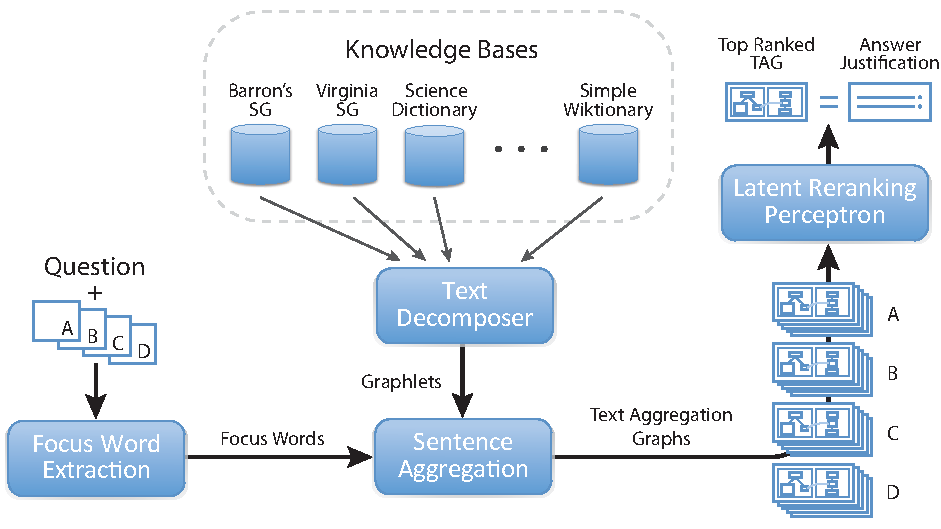
\includegraphics[width=1.0\textwidth]{mainmatter/tacl2015-tig/tag_architecture6c.pdf}

%space{-2mm}
\caption{Our QA approach, which centers on the construction of answer justifications as text aggregation graphs, and ranking them using a model that treats the justification quality as a latent variable.}
%space{-2mm}
\label{fig:architecture}
%\end{center}
\end{figure}

The architecture of our proposed QA approach is illustrated in Figure~\ref{fig:architecture}, and proceeds in a stage-like fashion.  

Prior to the QA task, in an offline process, we decompose sentences from six corpora into a lightly-structured graphical representation (``graphlet'') that splits sentences on clausal and prepositional boundaries (Section~\ref{sec-cl2017:tag}). As shown later, this is fundamental to the creation and evaluation of answer justifications.  All other stages of the framework occur online. 

The QA pipeline receives as input questions with multiple choice answers, similar to the questions shown in Table~\ref{tab:inferenceexamples}, and proceeds as follows. First, the questions are fed into a focus word extractor (Section \ref{sec-cl2017:focuswords}) that produces a weighted list of the keywords from both the question and answer candidates, sorted in descending order of their likely relevance to the information needed in the question. These keywords are used by the sentence aggregation component (Section \ref{sec-cl2017:tag}) to create an exhaustive list of potential answer justifications, for each answer candidate.  These answer justifications are in the form of text aggregation graphs (TAGs), each composed of two to three graphlets produced by the above preprocessing step.

After the sentence aggregation step, each of the multiple choice answers has a long list of candidate justifications.  Because of the large number of candidate justifications created for each question/answer pair (typically tens or hundreds of thousands), we filter the list to include only the top $k$ justifications based on an inexpensive score, implemented as the sum of the weights of the focus words present in each justification\footnote{We keep ties in this filtered list, which, due to the simplicity of the score, may increase the size of the filtered lists considerably. For example, if $k=25$, it is common that the filtered list includes between $100$ and $1,000$ candidate justifications.}. 
Using the focus words, we extract a number of features from each candidate justification that measure how well the justification answers the question (Section ~\ref{sec-cl2017:scoring}), and present this information to a latent-variable perceptron ranker (Section~\ref{sec-cl2017:perceptron}).  This learning framework learns which answer candidate is correct based on the candidate justifications, while also jointly learning to rank justification quality as a latent variable, selectively elevating good answer justifications to the top of the list.  

The candidate answer with the highest-scoring justification is taken to be the correct answer.  While the justification is expressed in the form of a text aggregation graph to make it easier to assemble and evaluate, we use the original sentences from the knowledge base used to construct that text aggregation graph as a human-readable justification for why that answer candidate is correct. 

\todo{remove focus word and TAG generation sections -- replace with summaries}
\section{Focus Word Extraction}
\label{sec-cl2017:focuswords}


%
% Focus word extraction example
%
\begin{table*}[t]
\caption{{Focus word decomposition of an example question, suggesting the question is primarily about measuring the speed of walking, and not about turtles or paths. (Correct answer: ``a stopwatch and meter stick.'') 
For a given word: 
\emph{Conc} refers to the psycholinguistic concreteness score,
\emph{Tag} refers to the focus word category (\emph{FOCUS} signifies a focus word, \emph{EX} an example word, \emph{ATYPE} an answer-type word, and \emph{ST} a stop word),
\emph{Score} refers to the focus word score, and
\emph{Weight} refers to the normalized focus word scores. 
}}
\begin{center}
\begin{footnotesize}
\addtolength{\tabcolsep}{-1.7pt}  
\begin{tabular}{r|cccccccccccc}
Words & What	& tools	& could & determine & the  & {\bf speed} & of   & turtles & {\bf walking} & along & a    & path ? 		\\
Conc  & 2.0A    & 4.6C  & 1.3A  & 2.1A      & 1.4A & {\bf 3.6}   & 1.7A & 5.0C    & {\bf 4.1}     & 2.1A  & 1.5A & 4.4C 		\\
Tag	  & ST      & ATYPE & ST    & ST        & ST   & {\bf FOCUS} & ST   & EX      & {\bf FOCUS}   & ST    & ST   & EX   		\\
Score & --      & 1     & --    & --        & --   & {\bf 14}    & --   & 2       & {\bf 14}      & --    & --   & 3			\\
Weight& --      & 0.03  & --    & --        & --   & {\bf 0.41}  & --   & 0.06    & {\bf 0.41}    & --    & --   & 0.09		\\
\end{tabular}
\addtolength{\tabcolsep}{1.7pt}  
\end{footnotesize}

\label{tab:focusexample}
\end{center}
\end{table*}


Questions often contain text that is not strictly required to arrive at an answer, and that can introduce noise into the answering process. 
This is particularly relevant for science exams, where questions tend to include a narrative or example for the benefit of the reader, and this extra text can make determining a question's \emph{information need} more challenging. 
%
%Elementary science exam questions are often crafted to test a student's knowledge of a single concept, process, or model.
%While some exam questions are short and direct {\em (e.g. What does a thermometer measure?)}, others embed the question in a narrative or example, and we first have to distill what the question is about before we're able to answer.  
For example, the question in Table~\ref{tab:focusexample} could be simplified to {\em What tools can be used to measure speed?}, but instead grounds the question in an example about turtles walking along a path.  As a first step in answering, we need to identify whether the focus of the question is about {\em speed}, {\em turtles}, {\em walking}, or {\em paths}, so that we can appropriately constrain our intersentence aggregation, and decrease the chance of generating noisy or unrelated justifications. 

Note that the {\em focus word} terminology was first introduced in the context of factoid QA, where it represents the question word or phrase that is indicative of the expected answer type, which is then used to constrain the search for candidate answers~\cite{Harabagiu:00,Moldovan:2003:PIE:763693.763694}. For example, {\em capital} is the focus word in the question {\em What is the capital of France?}. This information is used to constrain the search for answers to  entities that are of names of cities. 
In contrast, such words (e.g., {\em tools} for the previous exam question) are often of low importance for multiple choice science exams, as this information is already implicitly provided in the multiple choice answers.  Instead, our task is to identify the central concept the question is testing (e.g., {\em  measuring speed}), and to eliminate words that are part of an example or narrative (e.g., {\em  turtle, path}) that are unlikely to contribute much utility (or, may introduce noise) to the QA process. However, because at a high level focus words identify the information need of a question, which is what we aim to do as well, we continue to use the same terminology in this work.

Our approach borrows from cognitive psychology, which suggests that elementary school students tend to reason largely with concrete concepts (i.e., those that are easy to mentally picture), because their capacity for abstract thinking develops much more slowly into adulthood (e.g., Piaget ~\citeyear{Piaget1954}).  Recently Brysbaert et al. ~\citeyear{brysbaert:2014} collected a large set of psycholinguistic concreteness norms, rating 40 thousand generally known English lemmas on a numerical scale from 1 (highly abstract) to 5 (highly concrete).  We have observed that highly abstract words (e.g., {\em expertise:1.6, compatible:2.3, occurrence:2.6)} tend to be part of a question's narrative or too abstract to form the basis for an elementary science question, while highly concrete words (e.g., {\em  car:4.9, rock:4.9, turtle:5.0)} are often part of examples.  Words that are approximately 50\% to 80\% concrete {\em (e.g., energy:3.1, measure:3.6, electricity:3.9, habitat:3.9)} tend to be at an appropriate level of abstraction for the cognitive abilities of elementary science students, and are often the central concept that a question is testing.\footnote{
While the above concreteness thresholds may be particular to elementary science exams, we hypothesize that the information need of a question tends to be more abstract than the examples grounding that question.  We believe this intuition may be general and applicable to other domains.
}

Making use of this observation, we identify these focus words with the algorithm below. The algorithm is implemented as a sequence of ordered sieves applied in decreasing order of precision~\cite{Lee:13}. Each of the five sieves attempts to assign question words into one of the following categories\footnote{This same process is used to extract focus words for each of the multiple choice answer candidates, though it is generally much simpler given that the answers tend to be short.}: 

\begin{enumerate}

\item {\bf Lists and sequences:} Lists in questions generally contain highly important terms.  We identify comma delimited lists of the form {\small {\tt X, Y, ..., <and/or> Z}} (e.g., {\em sleet, rain, and hail}). Given the prevalence of questions that involve causal or process knowledge, we also identify from/to sequences (e.g., {\em from a solid to a liquid}) using paired {\tt prep\_from} and {\tt prep\_to} Stanford dependencies~\cite{de2008stanford}. 

\item {\bf Focus words:} Content lemmas (nouns, verbs, adjectives, and adverbs) with concreteness scores between 3.0 and 4.2 in the concreteness norm database of Brysbaert et al. ~\citeyear{brysbaert:2014} are flagged as focus words. 

\item {\bf Abstract, concrete, and example words:} Content lemmas with concreteness scores between 1.0 and 3.0 are flagged as highly abstract, while those with concreteness scores between 4.2 and 5.0 are flagged as highly concrete.  Named entities recognized as either durations or locations (e.g., {\em In New York State}) are flagged as belonging to examples.  

\item {\bf Answer type words:} Answer type words are flagged using both four common syntactic patterns shown in Table~\ref{tab:answertypewords}, as well as a short list of transparent nouns (e.g., {\em kind, type, form}). 

\item {\bf Stop words: } A list of general and QA-specific stop words and phrases, as well as any remaining words not captured by earlier seives, are flagged as stop words.

\end{enumerate}

\begin{table*}[t]
\caption{{Syntactic patterns used to detect answer type words.  Square brackets represent optional elements. }}
\begin{center}
\begin{footnotesize}
\begin{tabular}{ll}
\hline
\multicolumn{1}{l}{Pattern} & \multicolumn{1}{l}{Example} 	\\
\hline
(SBARQ (WHNP (WHNP (WDT) {\bf (NN)) [(PP)]}...						& What {\em kind of energy} ...    	\\
(SBARQ (WHNP (WP)) (SQ (VBZ is) {\bf (NP)}...	 					& What is {\em one method} that ... 	\\
(S (NP (NP (DT A) {\bf (NN)}) (SBAR (WHNP (WDT that)) ...			& A {\em tool} that ..					\\
(S (NP {\bf (NP)} (PP)) (VP (VBZ is) ...    						& The {\em main function} of ... is to ...	\\

\end{tabular}
\end{footnotesize}

\label{tab:answertypewords}
\end{center}
\end{table*}





{\flushleft {\bf Scoring and weights:}} We then assign a score to each question word based on its perceived relevance to the question as follows. 
Stop words are not assigned a score, and are not included in further processing.
All answer type words are given a score of 1.  Words flagged as abstract, concrete, or example words are sorted based on their distance from the concreteness boundaries of 3.0 (for abstract words) or 4.2 (for concrete words), where words closer to the concreteness boundary tend to be more relevant to the question, and should receive higher scores.
These words are then given incrementally increasing scores starting at 2 for the most distant word, and increasing by one until all words in this category have been assigned a score.
To create an artificial separation between focus words and the less relevant words, and to encourage our intersentence aggregation method to preferentially make use of focus words, we assign all focus words a uniform score 10 points higher than the highest-scoring abstract, concrete, or example word.  
Finally, list words, the most important category, receive a uniform score one higher than focus words.  The scores of all words are converted into weights by normalizing the scores to sum to one. 
An example of the scoring process is shown in Table~\ref{tab:focusexample}. 

It is important to note that the proposed focus word extraction algorithm is simple and leaves considerable room for improvement. We hypothesize that better algorithms could be implemented by switching to a learning-based approach. However, the simple unsupervised algorithm proposed requires no data annotations, and it captures the crucial intuition that some words in the question  contribute more towards the overall information need than others.  We demonstrate that this has a considerable impact on the performance of our overall QA system in the ablation studies discussed in Section~\ref{sec-cl2017:controls}.





\section{Text Aggregation Graphs}
\label{sec-cl2017:tag}

\begin{figure}[t!]
\begin{center}
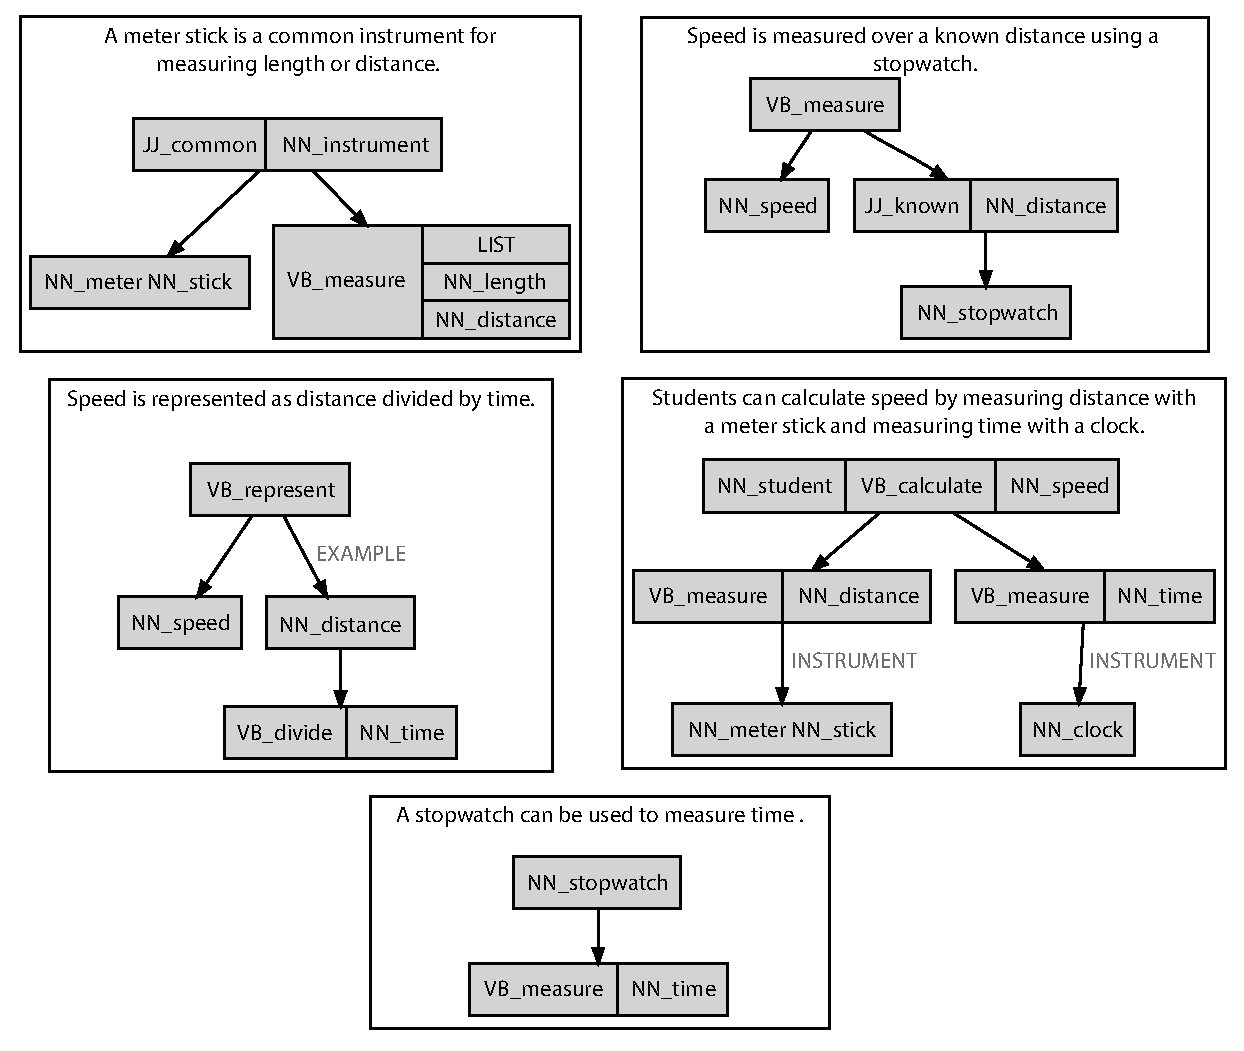
\includegraphics[width=115mm]{mainmatter/tacl2015-tig/example_graphlets1.pdf}
%	\centering
%	\begin{minipage}[b]{0.4\textwidth}	
%		\includegraphics[scale=0.4]{meter_length_distance.pdf}
%	\end{minipage}
%	\hfill
%	\begin{minipage}[b]{0.4\textwidth}	
%		\includegraphics[scale=0.4]{speed_distance_stopwatch.pdf}
%	\end{minipage}
%
%
%	\begin{minipage}[b]{0.4\textwidth}	
%		\includegraphics[scale=0.4]{speed_distance_time.pdf}
%	\end{minipage}
%	\hfill
%	\begin{minipage}[b]{0.4\textwidth}	
%		\includegraphics[scale=0.4]{speed_meter_clock.pdf}
%	\end{minipage}
\end{center}	
%space{-2mm}
\caption{Five example graphlets for five sentences that could be aggregated together in different combinations to justifiably answer the question \emph{What tools could determine the speed of turtles walking along a path? (Answer: stopwatch and meter stick)}.  Each graphlet contains one or more information nuggets (grey boxes) composed of one or more terms.  For example, the graphlet for the sentence \emph{A stopwatch can be used to measure time} contains two information nuggets.  Edges between nuggets within a graphlet are shown with arrows, where a subset of these edges are labelled (e.g., \emph{EXAMPLE, INSTRUMENT}), and the rest are unlabelled. 
}
%space{-5mm}
\label{fig:conceptexamples}
%\end{center}
\end{figure}




Semantic drift, or the tendency for a graph traversal to drift to unrelated topics,
constitutes a major hurdle for lexical semantic QA models.  
This was noted recently by Fried et al.~\citeyear{fried2015higher}, who proposed an approximation of inference for QA as the traversal of a graph that connected concepts (words or lexicalized syntactic dependencies) along lexical semantic associations. While this method is robust and performs better than approaches relying on alignment or embedding models alone, it does not have a good way of keeping an inference on-context when traversing the concept association graph.
Moreover, even when a correct answer is selected, these methods operate on sets of probabilities over word distributions, and are unable to provide a compelling human-readable explanation to the user as to why a given answer is correct. 

To address these issues, we propose to construct multi-sentence answer justifications using a  sentence aggregation method that combines the robustness of word-level connections with sentence-level context.  
Our approach works in two steps, both of which are performed offline, i.e., before the actual QA process. First, we decompose sentences that are likely to justify science exam answers (e.g., from knowledge bases such as study guides) into smaller units based on clausal and prepositional phrase boundaries. Intuitively, this allows us to maintain sufficient context to control semantic drift, while, at the same time, mitigating the sparsity of complete sentences.  
Following previous QA terminology, we call these smaller units,  which represent clauses or prepositional phrases, {\bf information nuggets}~\cite{Voorhees:2003}. We connect two information nuggets within the same sentence if there are any syntactic dependencies that connect any words in these nuggets. We call the resulting graph of these information nuggets, which represents an entire sentence, a \textbf{graphlet}. 
Figure \ref{fig:conceptexamples} shows a number of example graphlets. 
Formally, we transform sentences into graphlets using the following algorithm:


\begin{enumerate}

\item{\textbf{Parse knowledge base sentences: } 
All knowledge base sentences are syntactically parsed using the Stanford CoreNLP toolkit~\cite{manning2014stanford}.}

% ms: let's use {\tt } for syntactic dependencies, and {\em } font for text.

\item {\textbf{Decompose sentences into information nuggets: \label{step:creatinggraphlets}} 
For each sentence, beginning at the root of the dependency graph, we traverse the dependency graph and segment the sentence into nuggets along clausal complements ({\tt ccomp, xcomp}), adverbial and relative clause modifiers ({\tt advcl, rcmod}), reduced non-finite verbal modifiers ({\tt vmod}), and a subset of empirically determined prepositional phrases.\footnote{The full list of prepositional dependencies along which we split is: {\tt prep\_with, prep\_through, prep\_from, prep\_to, prep\_as, prep\_into, prep\_by, prep\_in, prep\_such\_as, prep\_because\_of, prep\_over, prep\_on, prep\_between, prepc\_as, prepc\_by, prepc\_of, prepc\_with, prepc\_after, prepc\_for, prepc\_before, prep\_before, prep\_after, prep\_during, prepc\_during, prepc\_because\_of, prep\_without,} and {\tt prepc\_without}.}
}

\item {\textbf{Segment nuggets into terms: }
Each nugget is segmented into one or more terms.  A term is nominally a single word, but we join both noun compounds and lists into single terms.  Noun compounds (e.g., \emph{meter stick} in Figure \ref{fig:conceptexamples}) are detected using the {\tt nn} dependency tag, and lists of words (e.g., \emph{sleet, rain, hail, or snow}) are detected through the same patterns used by the focus word extractor (see Section \ref{sec-cl2017:focuswords}).
}


\item {\textbf{Construct graphlets:} Two nuggets within a graphlet are connected if any of the words in one nugget have links in the syntactic dependency tree with words in the other nugget. } 

\item {\textbf{Label a subset of the graphlet  edges:} In general, to increase robustness, edges between nuggets are unlabelled.  The exceptions to this are a small set of high-confidence labels: the label {\tt definition} derived from the semi-structured dictionary resources which distinguish between a defined word and its definition, and the labels {\tt instrument, process, example, temporal}, and {\tt contrast} derived from prepositional dependencies.\footnote{More specifically, in our method the {\tt instrument} label corresponds to the dependencies {\tt prep\_with, prep\_through}, and {\tt prep\_by}.  The label {\tt process} corresponds to the dependencies {\tt prep\_from, prep\_to, prep\_into, prep\_because\_of}, and {\tt prepc\_because\_of}.  The {\tt example} label corresponds to {\tt prep\_as, prepc\_as, prep\_such\_as}, and {\tt prepc\_such\_as}.  The {\tt temporal} label corresponds to {\tt prep\_before, prepc\_before, prep\_after, prepc\_after, prep\_during} and {\tt prepc\_during}.  Finally, the {\tt contrast} label corresponds to {\tt prep\_without} and {\tt prepc\_without}.}}

\item {\textbf{Remove stop-words:}  Finally, we remove any stop words, as well as words that are not nouns, verbs, or adjectives.  Any nuggets that are empty after this filtering are removed. }

\end{enumerate}

\begin{figure}[t!]
\begin{center}

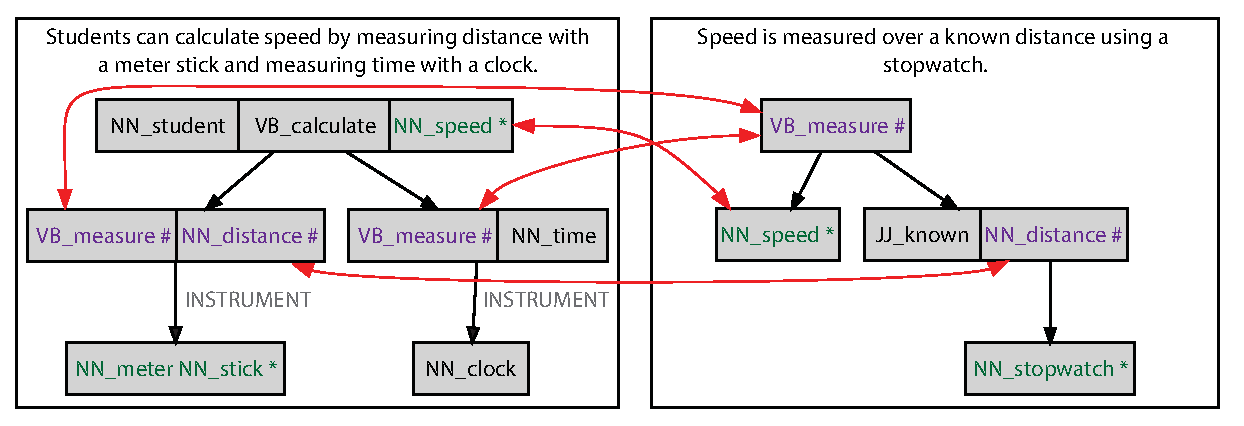
\includegraphics[width=115mm]{mainmatter/tacl2015-tig/tag_connection_example2.pdf}
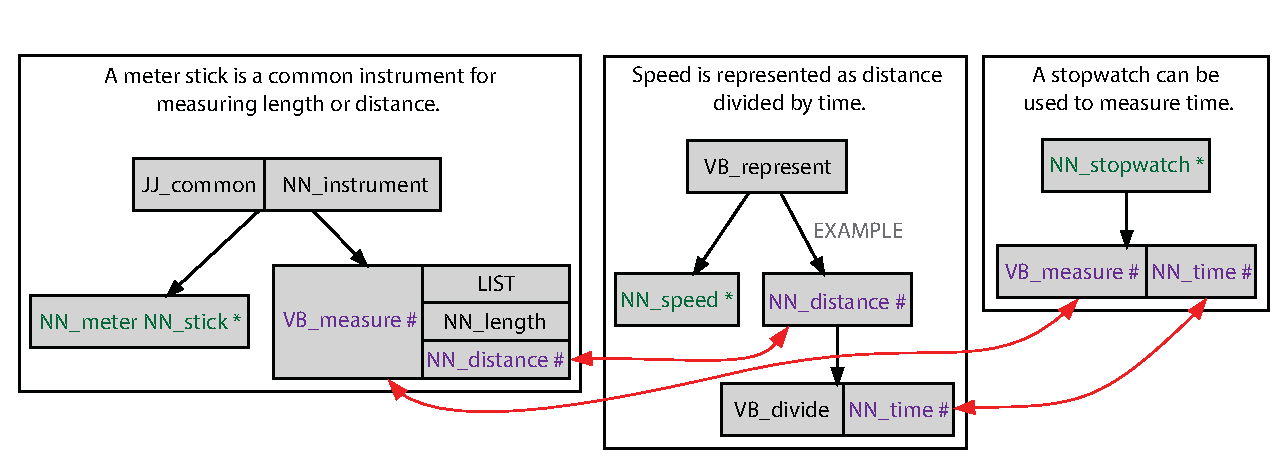
\includegraphics[width=115mm]{mainmatter/tacl2015-tig/tag_example2.pdf}

%space{-2mm}
\caption{
Two example Text Aggregation Graphs (TAGs) that justifiably answer the question \emph{What tools could determine the speed of turtles walking along a path} for the answer \emph{a stopwatch and meter stick}. Asterisks (*) denote that a given term is either a question or answer focus word, while pounds (\#) denote terms that are not found in the question or answer, but which are shared between graphlets.  Links between the graphlets in a given TAG are highlighted. (top) A two-sentence TAG, where the edges between graphlets connect on a focus word \emph{(speed)} and other words shared between the graphlets \emph{(distance, measure)}. (bottom) A three-sentence TAG, where the edges between graphlets connect entirely on shared words between the graphlets \emph{(distance, measure, time)} that are not focus words.
}
%space{-5mm}
\label{fig:tag_example}
\end{center}
\end{figure}


After the sentences have been transformed into graphlets, we construct candidates for multi-sentence justifications by connecting sentences with any lexical overlap between information nuggets.  We currently connect up to three graphlets into constructs we call \textbf{text aggregation graphs (TAGs)}, where each TAG corresponds to one potential answer justification. 
Figure~\ref{fig:tag_example} shows an example of two TAGs. 
Note that a TAG contains multiple levels of structure: (a) clause-level structure within nuggets, (b) sentence-level structure within graphlets, and (c) intersentence structure within TAGs\footnote{Currently, the graphlets and TAGs make use of lexical and syntactic structure only.  While this provides a robust representation of much of the structure in text, in a future system we would also like to explore adding semantic role and discourse information in our graphlets. Both of these have been shown to be useful, albeit for simpler QA tasks~\cite{Surdeanu:11,jansen14}.}.  
We will exploit this information in the next section, where we design features to capture the fitness of a TAG as a justification for a given answer.



\section{Text Aggregation Graph Features}
\label{sec-cl2017:scoring}

Once candidate answer justifications have been reframed as text aggregation graphs, the TAGs for each answer candidate need to be ranked such that a good justification for the correct answer will be ranked above all other answer justifications for incorrect answers. We describe the features that we extract from TAGs for this ranking in this section, and the latent ranking algorithm in Section~\ref{sec-cl2017:perceptron}.




\begin{table}[]
\caption{{  Features used to score candidate answer justifications represented as TAGs. }} 
\footnotesize{
\begin{tabular}{p{30mm}p{95mm}}
\hline
Feature & Description \\
\hline
\multicolumn{2}{l}{\emph{TAG-level features:}} \\
%numFocus			&	Number of unique Q and A focus words present in the TAG					\\
numFocusQ			&	Number of unique Q focus words present in the TAG						\\
numFocusA			&	Number of unique A focus words present in the TAG						\\
massFocusQ			&	Sum of the unique Q focus word weights present in the TAG				\\
massFocusA			&	Sum of the unique A focus word weights present in the TAG				\\
%\\
%\multicolumn{2}{l}{\emph{Other TAG-level Scores:}} \\
numRepeatedFocus	&	Number of focus words contained in more than one graphlet, with repetition \\
numOtherAnswerF		&	Negative predictor: the number of focus words from other multiple choice answers included in the current TAG.	\\
minConcShared		&	The minimum psycholinguistic concreteness score (i.e., abstractness) of any shared word in the TAG \\
\\
\multicolumn{2}{l}{\emph{Nugget-level features: }} \\
numNugF				&	Number of nuggets that are entirely focus words. \\
numNugFS 			&	Number of nuggets that contain only focus words and shared words. \\
numNugFSO			&	Number of nuggets that contain focus, shared, and other unmatched words. \\
numNugFO			&	Number of nuggets that contain only focus words and other words. \\
numNugS				&	Number of nuggets that contain only shared words. \\
numNugSO			&	Number of nuggets that contain only shared words and other words. \\
numNugO				&	Number of nuggets that contain only other words. \\
% \\
% \multicolumn{2}{l}{\emph{Other Nugget-level features: }} \\
numDefinedFocus		&	Number of nuggets containing only focus words with outgoing {\tt definition} edge \\
numDefinedShared	&	Number of nuggets containing only shared words with outgoing {\tt definition} edge \\
numQLinksFocus		&	Number of nuggets containing only focus words that have an incoming labeled link (e.g., {\tt definition, instrument, process, temporal})  \\
numQLinksShared		&	Number of nuggets containing only shared words that have an incoming labeled link  \\
numNuggetMultiF		&	Number of nuggets that contain more than one focus word\\
\\
\multicolumn{2}{l}{\emph{Bridge features:}} \\
massMaxBridgeScore		&	Bridge graphlets are graphlets that contain at at least one focus word from both the  \\
massMinBridgeScore		&	question and answer, signifying that they are highly relevant to the question and the \\
massDeltaBridgeScore	&	corresponding answer. A   graphlet's bridge score is the sum of this focus word mass.  We calculate the minimum, maximum, and delta (max $-$ min) bridge scores across all graphlets within a TAG. \\
\\



\hline
\end{tabular}
}
\label{tab:features}
\end{table}


\subsection {Features} 
\label{sec-cl2017:featuresandscoring}

We developed a set of TAG features that capture both the type of connections between the graphlets in a TAG, and how well the TAG as a whole relates to the corresponding question--answer pair.
The features can be broadly grouped into count features and mass features. Count features count the integer number of instances of a given event in a TAG -- for example, the number of nuggets that are entirely focus words.  Mass features sum the weights of focus words (as computed in Section~\ref{sec-cl2017:focuswords}) -- for example, summing the weight of all question or answer focus words found either within a single graphlet, or across the entire TAG.

A full list of the features and their descriptions can be found in Table \ref{tab:features}.
%
The features are grouped into three categories: TAG-level, nugget-level, and bridge features. 
The TAG-level features use focus words to evaluate the likelihood that an entire justification is relevant to the question and answer candidate. 
Nugget-level features provide a finer-grained measure of how well the individual sentences in a justification relate to each other by quantifying both \emph{how fully} they are connected (e.g., are all the words in a nugget matched with words in other nuggets, or only some), and what type of words they connect on (e.g., \emph{focus words}, or \emph{other words} not found in the question but shared between sentences).
Separate features encode whether a nugget is all focus words, all shared words, all unmatched words, or any partial combination of these three categories.
Finally, we define a graphlet that contains both question and answer focus words as a \emph{bridge graphlet}, in that its content tends to span or \emph{bridges} the question and answer, and include a set of bridge features for evaluating this subset of highly-relevant graphlets. 




%- TAG = path = answer justification
\begin{figure}[t!]
\begin{center}
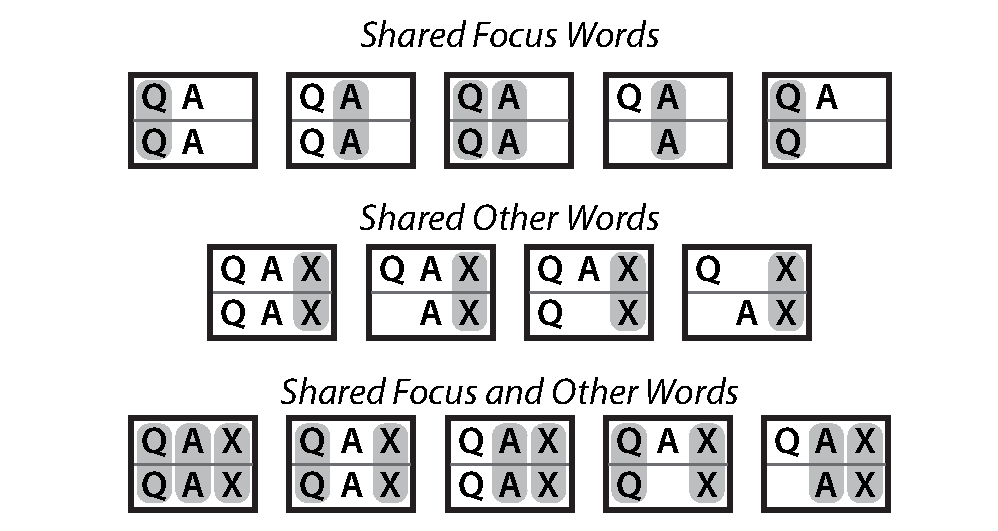
\includegraphics[width=75mm]{mainmatter/tacl2015-tig/connection_types.pdf}
%space{-2mm}
\caption{{Connections between sentences are characterized based on lexical overlap between graphlets.
Here, each box represents a two-sentence TAG, with graphlets stacked vertically.  The presence of question or answer focus words is marked with \emph{Q} or \emph{A}, while the presence of other non-focus words shared between the two graphlets is marked with \emph{X}.  Lexical overlap within a category is highlighted.
}}
%space{-5mm}
\label{fig:connectiontypes}
\end{center}
\end{figure}


\subsection {Modeling Different TAG Types Using Domain Adaptation} % Characterizing Lexical Overlap Between Sentences}
\label{sec-cl2017:characterizing}

Good justifications for an answer may take a variety of forms, from those with little lexical overlap due to the ``lexical chasm''~\cite{Berger:00} between question and answer, to those with a great deal of overlap. For example, of the two TAGs shown in Figure~\ref{fig:tag_example}, in the first TAG both sentences connect on question focus words, while in the second TAG the graphlets only connect on other non-focus words. 

Understanding the connections between sentences in a TAG serves as a robust proxy to modeling discourse structures (e.g., whether the second sentence elaborates on the concepts introduced in the first), which has been previously shown to increase both open-domain and science-domain QA performance~\cite{jansen14}.
This is important in the context of feature representations, because we conjecture that some features may be important across all the ways a justification can connect (so these features should be jointly modelled across connection types), whereas others are specific to certain connection types (so they should be modeled separately by type). As shown in Section~\ref{sec-cl2017:experiments}, this hypothesis is strongly empirically supported.

To model this phenomenon, we adapt a technique from the field of domain adaptation~\cite{daume2007}.
First, we label each of the sentences within a TAG based on whether they contain question focus words and/or answer focus words.  We then characterize the entire TAG by determining whether the words shared between sentences are question focus words, answer focus words, or other non-focus words.  This leads to 14 possible connection types, depicted in Figure \ref{fig:connectiontypes}.\footnote{In practice, for a configuration that allows TAGs of 1 or 2 sentences, we have 15 connection types, including the 14 two-sentence connection types, plus a single-sentence type. We ignore the single-sentence type in this discussion for simplicity, though it is included in our model.}
Second, following Daum{\'e}'s method, we generate 15 versions for each of the features introduced in Section~\ref{sec-cl2017:featuresandscoring}: a generic one that is type independent, and 14 that are affixed by each of the connection types. For example, for a given feature such as \emph{numFocusQ}, we create 15 copies: \emph{numFocusQ, numFocusQ$_1$ ... numFocusQ$_{14}$}, where the subscript (when present) indicates a specific connection type. For a TAG of connection type \emph{i}, only values for the type-specific feature \emph{numFocusQ$_i$} as well as the general feature \emph{numFocusQ} are populated -- all other \emph{numFocusQ$_j$} features are set to a value of zero. This allows the learning algorithm in the next section to learn whether each feature generalizes across connection types, or not. As shown in~\cite{finkel2010hierarchical}, this approach is equivalent to a joint model with a hierarchical prior. 



While the features introduced in Table~\ref{tab:features} apply to justifications containing any number of sentences, characterizing justifications that are longer than two sentences is not straightforward, as the number of connection types (Figure~\ref{fig:connectiontypes}) would become prohibitively large.   We handle three-sentence justifications by treating each as a set of three two-sentence TAGs, and characterize each two-sentence connection individually.  In the case where two groups of sentences have the same connection type, we take the highest scoring version of each overlapping feature.  While this method would extend to justifications of arbitrary length,  justifications longer than three sentences are not currently generated by our system. 



\section{Learning Model}
\label{sec-cl2017:perceptron}

We perform answer selection by focusing on ranking answer {\em justifications} rather then actual answers. 
Our algorithm (detailed in Algorithm \ref{alg:perceptron}) determines the best answer to a given question by first finding the highest-scoring TAG (i.e., justification) out of all the TAGs for each of its candidate answers, and then selecting the corresponding answer candidate.  
This introduces an additional complication during training: while we know which answer candidate is correct, the actual quality of any given TAG is hidden. That is, many TAGs which connect a correct answer to the question do so in the wrong context, producing a poor justification. Conversely, even an incorrect answer can be connected back to the question, otherwise the multiple choice test itself would be too easy. 

We address this issue with a reranking perceptron~\citep{Shen:Joshi:2005,Surdeanu:11} extended with a latent layer that models the correctness of the justifications. 
During training, we take advantage of the assumption that, with enough knowledge coverage, the best TAG for a correct answer will be better than the best TAG for an incorrect one.  As a result, our algorithm optimizes two goals jointly: choosing a good answer for a given question, and justifying it with a human-readable TAG that connects sentences from our knowledge bases.

\subsection {Learning Algorithm}
\label{sec-cl2017:model}

The input to the reranking algorithm consists of a corpus of $n$ training questions, $\boldsymbol{\mathcal{Q}}$, where each $q_i \in \boldsymbol{\mathcal{Q}}$ has a set of $m$ candidate answers, $\boldsymbol{A}$ (in the particular case of the multiple choice test, these are the four multiple choice answers).  Each $a_j \in \boldsymbol{A}$ for a given $q_i$ has a set of TAGs, $\boldsymbol{X_{i,j}}$, which connect $q_i$ to $a_j$.  
Crucially, for a correct answer, we assume that there is {\em at least one} valid TAG $x_c \in \boldsymbol{X_{i,j}}$, which justifies the correctness of the chosen answer. This assumption is similar to the one made by \citet{hoffmann2011knowledge}, who assumed that, for a binary relation extraction task, for each training relation between two entities, $e_1$ and $e_2$, there exists at least one correct sentence that supports the extraction of the given relation among the sentences that contain both $e_1$ and $e_2$.

The learning algorithm is formalized in Algorithm~\ref{alg:perceptron}. The two fundamental building blocks of the algorithm are the functions $P$ and $F$. 
Intuitively, the function $P$ identifies which justifications (or TAGs) for a given answer best explain the answer according to the current model. For example, for the question {\em Which organism is a producer?} and the answer {\em grass}, a good justification selected by function $P$ is a TAG that connects the two sentences: {\em Producer is an organism that produces its own food and is food for other organisms: usually a green plant.} and {\em Grass is a green, leafy plant that often covers the ground.} 
Because $P$ implements a latent operation (i.e., which justification is correct?), its goodness evolves together with the learned model. 
Note that, at this stage, we do not control how many justifications are produced by function P for a given answer other than constraining it to select {\em at least one}. The function $F$ computes the overall score of a given answer by simply averaging the scores of the justifications chosen by $P$. 

More formally, for a given question $q_i$ and candidate answer $a_j$, $P$ chooses a subset of TAGs from $\boldsymbol{X_{i,j}}$ that are deemed correct, according to the current model. $F$ averages the scores of these TAGs to compute the overall score of the answer $a_j$:

\begin{equation}
\label{eq:F}
F(q_i, a_j) = \frac{\sum_{x \in P(q_i, a_j)} \boldsymbol{\Theta} \cdot \Phi(x)}{|P(q_i, a_j)|}
\end{equation}
where the score of a given TAG, $x$, is computed as the dot product between the model's weight vector $\boldsymbol{\Theta}$  and the individual TAG's feature vector $\Phi(x)$. 

Given the functions $P$ and $F$ that control the latent operation of choosing valid answer justifications, the algorithm proceeds similarly to the reranking perceptron~\citep{Shen:Joshi:2005}. If a prediction, i.e., a choice for the correct answer for a given question (line 6), is incorrect (line 7), the algorithm updates its parameter vector, $\boldsymbol{\Theta}$, by adding all valid justifications of the correct answer as produced by $P$ (line 9), and subtracting all TAGs considered valid for the current top answer (line 12). 


The fundamental operation here is thus the implementation of $P$. For their classification task, Hoffman et al. implement this function as an edge-cover\footnote{
\rev{The edge-cover of a graph is a subset of the graph's edges such that each node in the graph is connected to at least one edge in the subset.  For the task of relation extraction, \citet{hoffmann2011knowledge} construct a fully-connected graph with nodes for each supporting sentence from the corpus and nodes for each relation.  Their approach to relation extraction learns which relations to extract from the supporting sentences by finding the \textit{best} edge-cover for the graph.}} problem, which guarantees that the overall score for the correct label (similar to our $F$ function) is maximized and at least one sentence supports the correct classification.  
For our reranking task, we found that a conservative interpretation of this, where {\em exactly} one justification is chosen, performed the best.\footnote{In fact, we found that performance consistently dropped as the number of justifications chosen by $P$ increased.} That is, $P$ returns only the top TAG with the highest score according to the dot product with the current $\boldsymbol{\Theta}$. 
We discuss the other extreme, i.e., using all TAGs, in Section \ref{sec-cl2017:controls} (when taken to this level, the latent layer is essentially disregarded entirely, assuming that each TAG for a correct answer is correct, and that each TAG for an incorrect answer is incorrect).  As discussed there, this performed far worse.


%\begin{algorithm}[t]
%%\SetAlgoLined
%%\linesnumbered
%\LinesNumbered
%\KwIn{  $ $\\
%$T$ -- the number of training epochs\;
%$\boldsymbol{\Sigma}$ -- the set of $n$ training questions, each of which has $m$ answer candidates\;
%$\boldsymbol{X_{i,j}}$ -- the set of all paths connecting a question $q_i$ with a candidate answer $a_j$\;}
%\KwOut{ \\
%$\boldsymbol{\Theta}$ -- parameter vector\;}
%\Begin{
%% {\small \tcp{Initialize parameter vector}}
%$\boldsymbol{\Theta} = \boldsymbol{0}$\;
%\For{$t\leftarrow 1$ \KwTo $T$}{
%	\For{$i\leftarrow 1$ \KwTo $n$} {
%			$k = \argmax_{j = 1, \dots, m} F(q_i, a_j)$\; 
%			\If{$k \ne 1$}{
%				\For{$x \leftarrow P(q_i, a_1)$}{
%					$\boldsymbol{\Theta} = \boldsymbol{\Theta} + \Phi(x)$\;
%				}
%				\For{$x \leftarrow P(q_i, a_k)$}{
%					$\boldsymbol{\Theta} = \boldsymbol{\Theta} - \Phi(x)$\;
%				}
%			}
%%			compute $ y_1 = F(a_1, X_1)$\\
%%			\For{$j\leftarrow 2$ \KwTo $m$} {
%%				%$z_{j}^{*}$ = $ argmax_{\bar{z_{j}}}$($\theta \cdot \bar{z_{j}}$)\; 
%%				compute $ y_j = F(a_j, X_j)  $\; 
%%				}
%%		find $p = argmax_m(Y) $\\
%%		\If{$ (y_1 - y_{p}) < \lambda $}{
%%			$ \bar{\theta} = \bar{\theta} + (\Phi(X_1) - \Phi(X_{p})) \tau $ \;
%%		}
%}
%}
%}
%\Return{$\boldsymbol{\Theta}$}
%\vspace{5mm}
%\caption{{\footnotesize Learning algorithm for the latent reranking perceptron. We consider, without loss of generality, that the correct answer appears at position 1 in training.}}
%\label{alg:perceptron}
%\end{algorithm}
\begin{algorithm}[t]                      % enter the algorithm environment
                 % and a label for \ref{} commands later in the document
\begin{singlespace}
                 \small
\begin{algorithmic}[1]                    % enter the algorithmic environment
    \STATE \textbf{Input:}{$ $\\
$T$ -- the number of training epochs}\\
$\boldsymbol{\mathcal{Q}}$ -- the set of $n$ training questions, each of which has $m$ answer candidates\\
$\boldsymbol{X_{i,j}}$ -- the set of all TAGs connecting a question $q_i$ with a candidate answer $a_j$\\
    \STATE \textbf{Output:}{ $\boldsymbol{\Theta}$ -- parameter vector\\}
    \STATE $\boldsymbol{\Theta} = \boldsymbol{0}$\;
	\FOR{$t\leftarrow 1$ --to-- $T$}
		\FOR{$i\leftarrow 1$ --to-- $n$} 
			\STATE $k = \argmax_{j = 1, \dots, m} F(q_i, a_j)$
			\IF{$k \ne 1$}
				\FOR{$x \leftarrow P(q_i, a_1)$}
					\STATE $\boldsymbol{\Theta} = \boldsymbol{\Theta} + \Phi(x)$
				\ENDFOR
				\FOR{$x \leftarrow P(q_i, a_k)$}
					\STATE $\boldsymbol{\Theta} = \boldsymbol{\Theta} - \Phi(x)$
				\ENDFOR
			\ENDIF
		\ENDFOR
	\ENDFOR
	\RETURN $\boldsymbol{\Theta}$
\end{algorithmic}
\end{singlespace}
\caption{ Learning algorithm for the latent reranking perceptron. We consider, without loss of generality, that the correct answer appears at position 1 in training.}   
\label{alg:perceptron}
\end{algorithm}



{\flushleft{\bf Inference:}}
%\paragraph{Inference}
During inference, the algorithm ranks all candidate answers for a given question in descending order of their score (as given by $F$, but using the averaged parameter vector, $\boldsymbol{\Theta_{avg}}$) and returns the top answer.

{\flushleft{\bf Practical concerns:}}
Two practical issues were omitted in Algorithm~\ref{alg:perceptron} for clarity, but improved performance in practice. First, we used the averaged percetron at inference time~\citep{Collins:2002:DTM}. That is, instead of using the latest $\boldsymbol{\Theta}$ after training, we averaged all parameter vectors produced during training, and used the averaged vector, $\boldsymbol{\Theta_{avg}}$, for inference.

Second, we used a large-margin perceptron, similar to~\citet{Surdeanu:11}. In particular, we update the model not only when the predicted answer is incorrect (line 5), but also when the current model is not confident {\em enough} -- that is, when the predicted answer is correct, but the difference in $F$ scores between this answer and the second predicted answer is smaller than a small positive hyper parameter $\tau$. 




\section{Experiments}
\label{sec-cl2017:experiments}

\subsection{Data}
\label{sec-cl2017:data}


{\flushleft {\bf Questions:}} We assembled a corpus of 1,000 third to fifth grade standardized elementary school science exam questions, consisting of 346 publicly available questions gathered from standardized exams in 12 states, as well as 654 additional questions from an exam generating service that are not publicly available. 
All questions are multiple choice with four possible answer candidates. Questions vary in length from 1 to 6 sentences, while the four multiple choice answer candidates are generally either single words or short phrases. 
Because of the small size of this corpus, our models were evaluated using 5-fold crossvalidation, with 3 folds for training, one for development, and one for test. 

{\flushleft {\bf Knowledge bases:}} Sentences from six text resources served as input for TAG generation.  Five of these resources are in the science domain and include two state-specific science exam study guides, a teacher's manual, a children's science dictionary, and a set of exam review flashcards.  Each of these in-domain resources was selected to be at a third-to-fifth grade knowledge level, and contained between 283 and 1,314 sentences (for a total of 3,832 in-domain sentences).  
The Simple Wiktionary\footnote{\url{http://simple.wiktionary.org}} was included as a large open-domain dictionary resource written at knowledge level similar to that of the exam questions.  Starting with over 24,000 definitions, we filtered these to include only definitions for nouns, verbs, and adjectives, for a total of 17,473 sentences after filtering.

\subsection{Tuning}
\label{sec-cl2017:tuning}
We tuned the following hyperparameters once on the development data to optimize both performance and stability.

{\flushleft \textbf{Number of candidate justifications:}} 
Each of the multiple choice answers can have a large number of candidate justifications.  To reduce runtime and assist learning, we filter this initial list of TAGs to include only a subset of TAGs with a high focus word mass. We kept all justifications tied for focus mass with the justification in 25th place, resulting in a variable number of TAGs for each QA pair.  For our dataset, the mean number of TAGs for each QA pair was 141. \\

{\flushleft \textbf{Perceptron Hyperparameters:}} We investigated the perceptron hyperparameters using a coarse grid search\footnote{For each hyperparameter, we systematically tried values differing by an order of magnitude (rather than by small increments) to find our final settings.} and found a stable optimum with 10 epochs, a $\tau$ of 1.0, burn in of 5 epochs (i.e., the weight updates were not added to the average weights for the first five epochs), and a learning rate (which dampened the updates to the weight vector) of 0.1. Since model results can vary depending on the random seed used for initialization, rather than using a single perceptron we use an ensemble of 50 perceptron models initialized with random weights.  These models are combined in a by voting -- each model casts a single vote for an answer candidate to each question (distributing the vote only in the case of ties), then the answer candidate with the most votes is selected.\\

{\flushleft \textbf{Feature Normalization:}} To minimize the effect of outliers in the feature space, we log-transformed the feature values, and then rescaled each feature independently to lie within the range of $-1$ to $1$, using the formula
\mbox{$normalized  = lower + (original - min)\frac{(upper - lower)}{(max - min)}$},
where $upper$ and $lower$ are the desired boundaries for the normalization ($1$ and $-1$, respectively), $max$ and $min$ are the maximum and minimum values for the corresponding feature across the training dataset, and $normalized$ is the result of normalizing $original$.
Note that during testing it is possible to see feature values outside of their known $[min, max]$ interval, which means that after normalization their values will fall outside the $[-1, 1]$ interval. We do not do any additional post-processing for these values.


\subsection{Baselines}
\label{sec-cl2017:baselines}

We include the following baselines: 

{\flushleft {\bf Random:}} selects an answer randomly.
{\flushleft {\bf Information retrieval (IR):}} ranks answers using an approach similar to the baseline model in \citet{jansen14}, which uses features that measure cosine similarity over {\em tf-idf} vectors \citep[][Ch. 6]{manning08} to rank answer candidates in a ``learning to rank'' (L2R) framework (see also Section \ref{sec-naacl2015:models}).  
Traditionally, with retrieval systems, short answers to questions are dynamically constructed from larger parent documents, and the top-scoring answer (defined as the answer with the highest {\em tf-idf} score between that answer candidate and a query vector made from the question) is taken to be the winner.  Here we adapt this setup to multiple choice exams by: (a) using query vectors that contain words from both the question and multiple choice answer candidate, and (b) generating features from the top {\em tf-idf} score for each answer candidate in a given question, which are then combined in the learning-to-rank framework.  We then take the short passage retrieved by the system as a justification for why that answer candidate is correct. 

Documents are constructed across the six knowledge bases by dividing each corpus by subsection (for texts), by definition (for dictionaries), or by flashcard.  We implemented the document indexing and retrieval system using Lucene\footnote{\url{http://lucene.apache.org}}.  Each sliding window of $N$ sentences in a given document served as a potential answer justification. Using the development questions, we empirically determined that a two-sentence window performed best, though performance did not significantly differ for window sizes between one and five sentences.  This  model generates two features: a cosine similarity score between the query vector and the best-scoring candidate answer justification in a given corpus, and a linear model that combines this cosine similarity with the cosine similarity between the query vector and the entire document, blending both local (answer justification) and global (document) context. 

Because our six corpora are of different genres (study guide, teachers guide, dictionary, flashcards), domains (science-domain vs. open-domain), and lengths (300 to 17,000 sentences), we implement six separate {\em tf-idf} models, each containing documents only from a single corpus. We then combine the two retrieval features from each model (12 features total) into a ranking perceptron \citep{Shen:Joshi:2005,Surdeanu:11} to learn which knowledge bases are most useful for this task.  This ensemble retrieval model produces a single score for each multiple choice answer candidate, where the top-scoring answer candidate is selected as the winner.  The top-scoring answer justifications from each of the six retrieval models then serve as justifications. 


 
{\flushleft {\bf Jansen et al. (2014):}} the best-performing combined lexical semantic and IR model of \citet{jansen14}, which was shown to perform well for open domain questions.  Similar to the IR model, we adapted this model to our task by including six separate lexical semantics (i.e. word embedding) language models \citep{mikolov13,mikolov10}, each trained on one of the six knowledge bases.  Two features that measure the overall and pairwise cosine similarity between a question vector and multiple choice answer candidate vector are included.  The overall similarity is taken to be the cosine similarity of the composite vectors of both the question and answer candidate, obtained by summing the vectors for the individual words within either the question or answer candidate vectors, then renormalizing these composite vectors to unit length.  The pairwise similarity is computed as the average pairwise cosine similarity between each word in the question and answer candidate.  Two features from each of the six lexical semantics models are then combined with the two features from each of the IR models (24 features total) as above using a ranking perceptron, with the top-scoring answer candidate taken as correct.  Because the lexical semantics features do not easily lend themselves to constructing answer justifications, no additional human-readable justifications were provided by this model. 


\subsection{Results}
\label{sec-cl2017:results}

Here we first investigate the performance of two variants of the TAG model with respect to justification length.  We then compare the best-performing model with the baselines, and show that the TAG and IR models can be combined to increase performance. We use the standard implementation for precision at 1 \citep[P@1;][]{manning08} and a tie-aware implementation of mean reciprocal rank \citep[MRR;][]{mcsherry2008}.  All statistical significance tests were performed using one-tailed bootstrap resampling with 10,000 iterations (see Section \ref{sec-naacl2015:results}, Footnote \ref{footnote:bootstrap} for implementation).



%
% Performance versus path length
%
\begin{table}[t]
\small
\begin{center}
%\begin{tabular}{p{0.3mm}p{55mm}llll}
\begin{tabular}{lllll}
\multicolumn{1}{l}{ } & \multicolumn{1}{l}{ } & \multicolumn{1}{l}{P@1} & \multicolumn{1}{l}{ } & \multicolumn{1}{l}{MRR} \\
\multicolumn{1}{l}{ Model } & \multicolumn{1}{l}{P@1} & \multicolumn{1}{l}{Impr.} & \multicolumn{1}{l}{MRR} & \multicolumn{1}{l}{Impr.} \\
\hline
\multicolumn{5}{l}{Normal}\\
\hline
1G					& 35.33			& --				& 59.26  		&	--  \\
2G					& {\bf 38.16}	& {\bf 8.0\%}	& {\bf 61.33}  	&	{\bf 3.5\%}  \\
3G					& 37.78			& 6.3\%			& 61.14  		&	3.2\%  \\
\\
\hline
\multicolumn{5}{l}{Connection-type aware (Daum{\'e})}\\
\hline
1G\textsubscript{CT}			& 34.80			& --				& 58.86  		& --  \\
2G\textsubscript{CT}			& {\bf 39.91}	& {\bf 14.7\%}	& {\bf 62.53}  	& {\bf 6.2\%} \\
3G\textsubscript{CT}			& 38.53			& 10.7\%			& 61.65  		& 4.7\%  \\

\hline
\end{tabular}
\caption{{
Performance as a function of justification length in sentences (or, the number of graphlets in a TAG) for two models: one aware of connection-type, and one that is not. Bold font indicates the best score in a given column for each model group. 
}}
\label{tab:pathlength}
\end{center}
\end{table}


\subsubsection{Justification Length}
\label{sec-cl2017:pathlength}
Table~\ref{tab:pathlength} shows the performance of the TAG model as a function of increasing justification length.
Here, the $k$G models contain exclusively justifications of length $k$ (we explore TAGs of varying length later in this section).
Short two-sentence (or two-graphlet) TAGs significantly outperform single sentence TAGs, with single sentence (1G) TAGs starting at 35.3\% P@1, increasing to 38.2\% for two-sentence (2G) TAGs, hen decreasing slightly to 37.8\% for three-sentence (3G) TAGs. 
In previous work, we observed that for a variety of word-level graphs and traversal algorithms, QA performance tends to rapidly peak when aggregating two or three words, then slowly decreases as more words are aggregated due to ``inference drift'' in the graph 
traversal process
(i.e., following the connections from \emph{breakfast} $\rightarrow$ \emph{hashbrowns} $\rightarrow$ \emph{potato} $\rightarrow$ \emph{field} would potentially connect questions about breakfast to information about potato or even soccer fields)   \citep{fried2015higher}.  

Though our sentence aggregation model contains far more structure than the higher-order lexical semantic graphs of \citet{fried2015higher}, and is represented at the level of the sentence or graphlet rather than individual lemmas, we hypothesize based on this previous work that we may be observing the beginning of same characteristic peak in performance reported there.  Because runtime increases exponentially with the number of sentences included in a TAG, it quickly becomes intractable to test this with TAGs containing more than 3 graphlets. 

Extending the model to include a knowledge of the connection type (or the type of lexical overlap, see Section~{\ref{sec-cl2017:characterizing}) between sentences in a given TAG using Daum{\'e}'s method~\citep{daume2007} increases performance, suggesting that different kinds of connections are best identified through different feature patterns.  Here, the connection-type aware 2G\textsubscript{CT} model outperforms the regular 2G model by nearly 2\% P@1 (absolute), increasing performance to 39.9\% -- an increase of +14.7\% (relative) over using only single-sentence TAGs.\footnote{Each of the 50 models in the ensemble reranker is initialized with random weights, causing the small performance difference between 1G and 1G\textsubscript{CT}}





\subsubsection{Combined Models}
\label{sec-cl2017:combinedmodels}
%
% Combined model performance
%
\begin{table*}[t]
    \small
\begin{center}
\begin{tabular}{p{0.3mm}p{55mm}llll}
\multicolumn{1}{l}{ } & \multicolumn{1}{l}{ } & \multicolumn{1}{l}{ } & \multicolumn{1}{l}{P@1} & \multicolumn{1}{l}{ } & \multicolumn{1}{l}{MRR} \\
\multicolumn{1}{l}{\#} & \multicolumn{1}{l}{ Model } & \multicolumn{1}{l}{P@1} & \multicolumn{1}{l}{Impr.} & \multicolumn{1}{l}{MRR} & \multicolumn{1}{l}{Impr.} \\

\hline
& \multicolumn{5}{l}{Baselines }\\
\hline
1 & Random					& 25.00 			& --		& 52.08  		& --	  \\
2 & IR 						& {\bf 40.20} 	& -- 	& {\bf 62.49}	&	--  \\
3 & Jansen et al. (2014)		& 37.30 			& --		& 60.95 			& 	--	 \\

\\
\hline
& \multicolumn{5}{l}{Combined models with justifications of variable lengths (Single classifier)}\\
\hline
4 & 1G + 2G										& 38.69			& --		& 61.43  	& --  \\
5 & 1G\textsubscript{CT} + 2G\textsubscript{CT} 	& {\bf 42.88$\dagger ^4$}	& {\bf +6.7\%}		& {\bf 63.94\%}  	& {\bf +2.3\%}	  \\

\\
\hline
& \multicolumn{5}{l}{Combined models that include the IR baseline (Voting)}\\
\hline
6 & IR $\cup$ 1G\textsubscript{CT} $\cup$ 2G\textsubscript{CT} $\cup$ 3G\textsubscript{CT} 			& 43.15*			& +7.3\%			& 64.51*		& +3.2\%	  \\
7 & IR $\cup$ (1G\textsubscript{CT} + 2G\textsubscript{CT}) $\cup$ 3G\textsubscript{CT} 			& {\bf 44.46**}		& {\bf +10.6\%}		& {\bf 65.53**} 		& {\bf +4.9\%}	  \\

\hline
\end{tabular}
    \caption{{
Performance of the baseline and best-performing TAG models, both separately and in combination. TAG justifications of different short lengths were found to best combine in single classifiers (denoted with a $+$), where models that combine the IR baseline or long (3G) TAG justifications best combined using voting ensembles (denoted with a $\cup$). Bold font indicates the best score in a given column for each model group. Asterisks indicate that a score is significantly better than the highest-performing baseline model (* signifies $p < 0.05$, ** signifies $p < 0.01$).  The dagger indicates that a score is significantly higher than the score in the line number indicated in superscript ($p < 0.01$). All significance tests were implemented using one-tailed non-parametric bootstrap resampling using 10,000 iterations. }}
\label{tab:combinedmodels}
\end{center}
\end{table*}

Where Table~\ref{tab:pathlength} lists models that contain justifications of static length, \citet{fried2015higher} showed that combining paths of different lengths into a single classifier can increase performance.  The performance of TAG models that combine justifications of different lengths, as well as the baseline models, is shown in Table~\ref{tab:combinedmodels}.

{\flushleft {\bf Baselines:}} Where the lexical semantics model of \citet{jansen14} outperformed their IR baseline by +36\% (relative) on a large corpus of open-domain questions from Yahoo Answers, here on elementary science exams, the lexical semantic features decrease performance.  Our conjecture is that the performance difference is due to the difference in the size of the corpora used to train the lexical semantic model -- where Jansen et al. trained their lexical semantic model using Gigaword, here we are limited by the relatively small size of our text resources.  \citet{jansen14} reported that a domain-specific version of their lexical semantic model performed poorly when trained on a biology textbook and subset of Wikipedia, and others have since shown that lexical semantic models perform poorly with small amounts of training data \citep[][see also Chapter \ref{chapter:naacl2015}]{sharp-EtAl:2015:NAACL-HLT}. 

{\flushleft {\bf Combined Models:}} Single-classifier models containing both 1G and 2G TAGs were generated for both the normal and connection-type-aware models.  The 1G + 2G model performs only slightly better than 2G alone, but when the models are connection-type aware, there is greater benefit to combining the different path lengths -- the connection-type-aware 1G\textsubscript{CT} + 2G\textsubscript{CT} model (line 5) increases performance to 42.9\% P@1 (compare to the static-length 2G\textsubscript{CT} performance of 39.9\%).


As the IR baseline and the TAG models are performing inherently different tasks (information \emph{retrieval} and information \emph{aggregation} respectively), we are able to combine them together in a voting model in order to create a full system that contains the benefits of each.
The voting models that incorporate both the IR baseline and TAG models across all justification lengths are included on lines 6 and 7.  Both models significantly increase performance over the IR baseline, with the voting model that couples 1G\textsubscript{CT} + 2G\textsubscript{CT} as a single classifier (and single vote) performing better than when 1G\textsubscript{CT} and 2G\textsubscript{CT} vote separately.  This best-performing model reaches 44.5\% P@1, increasing performance over the IR baseline by +10.6\% (relative). %All in all
This set of experiments demonstrates that our approach of jointly ranking answers and justifications is complementary to a strong information retrieval baseline, and significantly improves performance at the task of selecting the correct answer.  


\subsubsection{Justifications}


%
% Justification example (IR)
%
\begin{table*}[t]
\begin{center}
\begin{footnotesize}
%\begin{tabular}{lcc}
%\cline{2-3}
%\begin{tabular}{cl}
\begin{tabularx}{\textwidth}{p{1cm}p{11.5cm}}
%\multicolumn{1}{r}{} & \multicolumn{1}{l}{} \\
%\cline{1-2}
%\hline
\hline
\multicolumn{1}{c}{} & \multicolumn{1}{c}{Question} \\
\hline			
\multicolumn{2}{l}{	What is the interaction between the producer and the consumer in a food chain?} \\
		&	\textbf{[A] The consumer eats the producer for energy.}  \\
		&  [B] The consumer does not interact directly with the producer. \\
			&   [C] The producer eats other producers for energy.   \\
			& [D] The producer eats the consumer for energy. \\
%Answer		&	The consumer eats the producer for energy. \\			

\multicolumn{1}{c}{} & \multicolumn{1}{c}{} \\				
\hline
\multicolumn{1}{l}{Rating} & \multicolumn{1}{c}{Example Justification} \\
\hline			
{\em Good }		&	A primary (1st) consumer eats producers (plants). A secondary (2nd) consumer eats primary consumers. {\em [Barrons SG]}  	\\
{\em Half }		&	The food chain starts with a producer (a plant) and ends with a decomposer. {\em [Flashcards]} \\
{\em Topical }	&   A herbivore is an organism that depends on plants for most of its food and energy. {\em [Science Dictionary]} \\
{\em Offtopic }	&	When a plate moves suddenly a great amount of energy is released.  These waves cause damage...  {\em [Virginia SG]} \\
%\end{tabular}
\end{tabularx}
\end{footnotesize}
\caption{{ Example justifications from the IR baseline and their associated ratings. }} %  (N=20, c=0.1)

\label{tab:justificationsIRexamples}

\end{center}
\end{table*}


%
% Justification example (TAG)
%
%\begin{figure}[t!]
%\begin{center}
%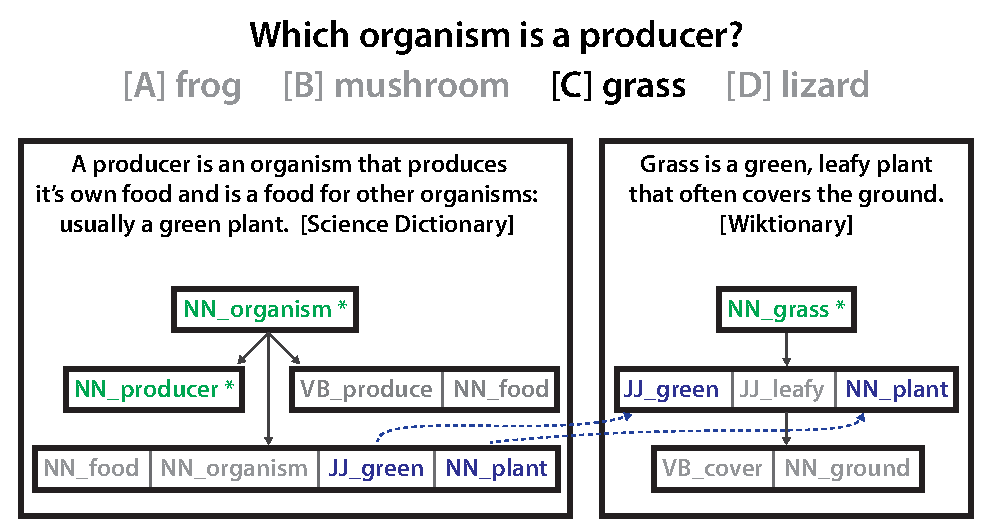
\includegraphics[width=75mm]{example_tig_producer2.pdf}
%\vspace{-2mm}
%\caption{ An example TAG path and justification rated as {\em good}. \note{TODO: Redraw figure with different line widths, closer to the original DOT file?}}
%%\caption{{\small An example of the alignments produced by the two discourse models.  The sequential model aligns pairs of consecutive sentences, capturing intersentence associations such as \emph{cider--apples}, and \emph{orchard--autumn}.  The RST model generates alignment pairs from participants in all (binary) discourse relations, capturing both intrasentence and intersentence alignments, including 
%%\emph{apples--orchard, cider--apples}, and \emph{cider--autumn}.}}
%% ms: I get the point, but there is value in brevity. Plus, maybe we should not use Bob as example :)
%%the intersentence alignments above along with intrasentence and multi-sentence alignments, including \emph{Bob--cider, apples--orchard}, and \emph{cider--autumn}.}}
%\vspace{-5mm}
%\label{fig:justificationTAGexample}
%\end{center}
%\end{figure}



\begin{table}[]
\small
\begin{tabularx}{\textwidth}{p{2.5cm}p{11cm}}
%\hline
%\multicolumn{2}{l}{EXAMPLE: Other} \\
\hline
% Question Info
Question & Which organism is a producer? (GR:5)     \\
Focus Word(s) &   (NN\_producer, 0.92) (NN\_organism, 0.08) \\
Answers & (A) frog  (B) mushroom   (C) grass    (D) lizard \\
\hline
% Correct Answer Info
Correct Answer &  grass \\
Focus Word(s) &   (NN\_grass, 1.00) \\
\multicolumn{2}{c}{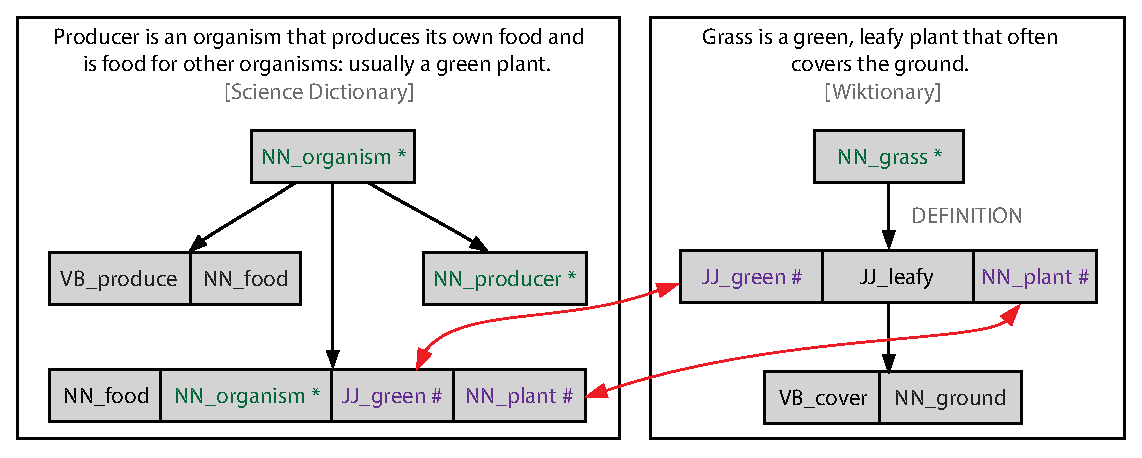
\includegraphics[width=115mm]{mainmatter/tacl2015-tig/tag_good_justification.pdf}}
\\
\hline
\end{tabularx}
\caption{{An example TAG and justification rated as {\em good}.  The two sentences connect on non-focus "other" shared words (e.g., \emph{green, plant}) which are not found in the question or answer, but which are highly related to the focus words. }} 

\label{ex:tagQsXs}
\end{table}






%
% Justification Examples - EXTRA
%
%\begin{table}[]
%\caption{{  Example of a TAG {\bf connected on answer focus} words. }} 
%\begin{tabularx}{\textwidth}{p{2.5cm}p{11cm}}
%%\hline
%%\multicolumn{2}{l}{EXAMPLE: Other} \\
%\hline
%% Question Info
%Question & What are the stages of development of an organism called? (GR:5)   \\
%Focus Word(s) &  (NN\_organism, 0.80) (NN\_stage, 0.13) (NN\_development, 0.07) \\
%\hline
%% Correct Answer Info
%Correct Answer &  Life cycle \\
%Focus Word(s) &  (NN\_cycle, 0.92) (NN\_life, 0.08) \\
%\multicolumn{2}{c}{\includegraphics[scale=0.5]{q58a1p2363connection.png}}\\
%\hline
%\end{tabularx}
%\label{ex:tagAns}
%\end{table}

%\begin{table}[]
%\caption{{  Example of a TAG {\bf connected on question and answer focus words}. (Somewhat more challenging focus word extraction, but we end up matching most of the words).  }} 
%\begin{tabularx}{\textwidth}{p{2.5cm}p{11cm}}
%%\hline
%%\multicolumn{2}{l}{EXAMPLE: Other} \\
%\hline
%% Question Info
%Question & Different types of organs that work together to perform a specific life function are called a(n) \_\_\_. (GR:5)   \\
%Focus Word(s) &   (VB\_work, 0.23) (VB\_perform, 0.23) (NN\_n, 0.23) (RB\_together, 0.09) (NN\_life, 0.07) (JJ\_specific, 0.06) (JJ\_different, 0.04) (NN\_function, 0.03) (NN\_organ, 0.01) \\
%\hline
%% Correct Answer Info
%Correct Answer &  organ system \\
%Focus Word(s) &   (NN\_system, 0.67) (NN\_organ, 0.33) \\
%\multicolumn{2}{c}{\includegraphics[scale=0.5]{q61a2p1104connection.png}}\\
%\hline
%\end{tabularx}
%\label{ex:tagQuest+Ans}
%\end{table}

%\begin{table}[]
%\caption{{  Example of a TAG connected only on answer focus words. Despite a non-ideal ranking of the question focus words, the system is able to lock onto this as a good justification of the correct answer.}} 
%\begin{tabularx}{\textwidth}{p{2.5cm}p{11cm}}
%%\hline
%%\multicolumn{2}{l}{EXAMPLE: Other} \\
%\hline
%% Question Info
%Question & Pots and pans are most often made from metal because \_\_\_. (GR:5)     \\
%Focus Word(s) &   (NN\_pot, 0.48) (NN\_pan, 0.48) (NN\_metal, 0.04) \\
%\hline
%% Correct Answer Info
%Correct Answer &  metals conduct heat well \\
%Focus Word(s) &   (NN\_heat, 0.44) (RB\_well, 0.44) (NN\_metal, 0.07) (VB\_conduct, 0.04) \\
%\multicolumn{2}{c}{\includegraphics[scale=0.5]{q100a3p908connection.png}}\\
%\hline
%\end{tabularx}
%\label{ex:tagXs}
%\end{table}

%\begin{table}[]
%\caption{{  {\bf Error example: Construction and Ranking vs Answer Selection:} Example of a question which requires {\bf complex inference}.  Our system aggregate sentences by connecting on {\bf question focus words as well as non-focus words}, to construct a good justification for the correct answer and rank it to the top of the justifications for that answer candidate. }} 
%\begin{tabularx}{\textwidth}{p{2.5cm}p{11cm}}
%%\hline
%%\multicolumn{2}{l}{EXAMPLE: Other} \\
%\hline
%% Question Info
%Question & In a food chain or web, the most efficient users of the Sun's energy are \_\_\_. (GR:5)     \\
%Focus Word(s) &   (NN\_chain, 0.23) (NN\_web, 0.23) (NN\_user, 0.22) (NN\_energy, 0.22) (NN\_food, 0.05) (NN\_sun, 0.03) (JJ\_efficient, 0.02) \\
%\hline
%% Correct Answer Info
%Correct Answer &  herbivores \\
%Focus Word(s) &   (NN\_herbivore, 1.00) \\
%\multicolumn{2}{c}{\includegraphics[scale=0.5]{q67a2p1connection.png}}\\
%\hline
%\end{tabularx}
%\label{ex:tagQsXsWrong}
%\end{table}
%
%
%\begin{table}[]
%\caption{{  {\bf Error example:} A similar example to the last one -- much of the time we're able to construct and rank very good TAGs (for a given answer candidate), but the last step -- selecting the best justification, is more sensitive to {\emph well connected answers} rather than {\emph good answers}.  Here the two aggregated sentences are {\bf connected on question focus words.}  }} 
%\begin{tabularx}{\textwidth}{p{2.5cm}p{11cm}}
%%\hline
%%\multicolumn{2}{l}{EXAMPLE: Other} \\
%\hline
%% Question Info
%Question & All organisms need food to survive. Which statement best describes the purpose of food for organisms? (GR:4)    \\
%Focus Word(s) &   (NN\_organism, 0.34) (NN\_organism, 0.34) (VB\_survive, 0.08) (NN\_food, 0.05) (VB\_need, 0.03) (NN\_food, 0.08) (NN\_purpose, 0.05) (NN\_statement, 0.03) \\
%\hline
%% Correct Answer Info
%Correct Answer &  Food provides energy for growth. \\
%Focus Word(s) &   (NN\_energy, 0.68) (NN\_growth, 0.16) (VB\_provide, 0.11) (NN\_food, 0.05) \\
%\multicolumn{2}{c}{\includegraphics[scale=0.5]{q19a3p2833connection.png}}\\
%\hline
%\end{tabularx}
%\label{ex:tagQsAsWrong}
%\end{table}
%
%
%
%\begin{table}[]
%\caption{{ {\bf Error example:} Another example of {\bf complex inference} that {\bf connects on other words}, in this case {\emph river}.  Again we're ranking this \todo{path} to the candidates for a given answer, but not selecting it out of the 4 multiple choice answers.  }} 
%\begin{tabularx}{\textwidth}{p{2.5cm}p{11cm}}
%%\hline
%%\multicolumn{2}{l}{EXAMPLE: Other} \\
%\hline
%% Question Info
%Question & Moving water was the most important factor in forming which of these? (GR:5)   \\
%Focus Word(s) &   (VB\_move, 0.68) (NN\_factor, 0.16) (NN\_water, 0.11) (JJ\_important, 0.05) \\
%\hline
%% Correct Answer Info
%Correct Answer &  the Grand Canyon \\
%Focus Word(s) &   (NN\_canyon, 0.67) (NN\_grand, 0.33) \\
%\multicolumn{2}{c}{\includegraphics[scale=0.5]{q33a0p57connection.png}}\\
%\hline
%\end{tabularx}
%\label{ex:tagXsWrong}
%\end{table}

The previous experiments demonstrate that our method performs well at identifying correct answers. But how well does it perform at the task of {\em justifying} those answers?
We evaluated justification performance for both the best baseline (IR) and the best performing TAG model that is independent of IR (i.e., 1G\textsubscript{CT} + 2G\textsubscript{CT}) .  Where TAG justifications took the form of the sentences being aggregated, justifications for the IR model were taken to be the highest-scoring short passages from each of the six knowledge bases.  As the IR model was tuned to a retrieval size of two sentences to maximize P@1 performance, each IR justification was two sentences in length.\footnote{Documents for the dictionary and flashcard corpora typically contained only a single sentence, and so answer justifications from these corpora are often shorter than two sentences.} To facilitate easy comparison, since the IR model provides six justifications (one from each knowledge base), we evaluate the top six scoring TAG justifications.  

Two of the authors independently rated the quality of the justifications. Any detected conflicts were resolved post hoc by the two annotators working together.
Answer justifications were rated on a four-point scale, based on their ability to provide a convincing justification to the user as to why a given answer choice was correct (see  Table~\ref{tab:justificationsIRexamples} for IR examples, and Figure~\ref{ex:tagQsXs} for a TAG example).   Justifications rated as {\em\bf good} describe the inference required to arrive at the correct answer.  Those rated as {\em\bf half} contained at least a portion of an explanation of the inference, but missed some critical aspect required to answer the question, like discussing producers but not consumers in Table~\ref{tab:justificationsIRexamples}. The two final ratings are for justifications that did not address the inference -- {\em\bf topical} justifications do not address the question but discuss a similar topic, where {\em\bf offtopic} justifications are unrelated to the question. 

%
% Justification performance
%
\begin{table}[t]
\small
\begin{center}
\begin{tabular}{p{20mm}cc}
\hline
\multicolumn{1}{l}{Rating} & \multicolumn{1}{c}{IR} & \multicolumn{1}{c}{TAG} \\%  & IR & TAG \\
\cline{2-3}
\hline
Good				&	45.3\%		& 56.7\%	 \\%	& 12.6\%		& 45.1\%	 \\
Half				&	34.9\%		& 20.7\%	 \\%	& 17.3\%		& 18.0\%	 \\
Topical			&	11.9\%		& 14.4\%	 \\%	& 17.2\%		& 18.4\% \\
Offtopic			&	7.9\%		& 8.2\%	 \\%	& 52.9\%		& 18.5\% \\

\end{tabular}
\caption{{ \emph{At least one} justification performance for both IR and TAG models, reflecting the highest rating attained by at least one of the top six justifications for a given question. }}%  Precision@6 performance reflects the overall proportion of each rating across all of the top six justifications. }} %  
\label{tab:justifications}

\end{center}
\end{table}

We evaluated the top-rated answer justifications using an {\bf at least one} method.  With this method, performance reflects the highest rating attained by \emph{at least one} of the six justifications for a given question. For example, for a question to be classed as {\em good}, at least one of the six answer justifications must be rated as {\em good}.  \emph{At least one} answer justification performance is listed in Table~\ref{tab:justifications}. For the TAG model, 56.7\% of the questions had at least one justification rated as {\em good}, outperforming IR justifications by 11.4\% (absolute).  


This experiment supports our original intuition that justifications must be aggregated from multiple resources. While the small window of sentences from the IR model is sufficient to justifiably answer many questions, a large number of questions require knowledge to be aggregated from {\em non-adjacent} sentences within a given corpus, or from sentences in different corpora altogether, to compose convincing answer justifications.  While the IR model leaves many of these questions with only partial justifications (34.9\% of justifications are rated as {\em half}), the TAG model  is able to aggregate sentences from multiple sources, and finds complete {\em good} justifications for many of the questions only partially answered by the IR model.


\subsubsection{Ablation Studies}
\label{sec-cl2017:controls}
To verify the contribution of the components of our system, we include the following ablation studies:
%\paragraph{How does the latent layer in the Ranking Perceptron affect performance?}
{\flushleft {\bf Latent Perceptron:}} The complete removal of the latent layer (i.e., using the average of all TAG scores to score the candidate answer, and performing perceptron updates with all TAGs) decreases the performance of the best performing TAG model (1G\textsubscript{CT} + 2G\textsubscript{CT}) from 42.88 to 35.43 P@1.  Alternatively, we experimented with using the sum of the TAG scores and the maximum TAG score as the candidate score, while still doing updates with all TAGs.  These configurations decreased performance to 34.46 and 38.09 P@1, respectively. This demonstrates the importance of modeling justification quality as a latent variable.

%\paragraph{How do the focus words impact performance?}
{\flushleft {\bf Focus Words:}} Focus words are used both to find relevant sentences to aggregate into answer justifications, as well as to characterize those justifications when expressed as TAGs. Replacing focus words with uniform weights for all content words (NN, VB, JJ) in a question reduces performance of the 1G+2G model from 38.69 to 33.89 P@1.  For the connection-type-aware model (1G\textsubscript{CT} + 2G\textsubscript{CT}), performance decreases from 42.88 to 40.03 P@1. This supports our observation that science exam questions contain several layers of information (e.g., the underlying question, and the example the question is grounded in), each contributing different utility to the QA process. 

%\paragraph{How does the graphlet structure impact performance?}
{\flushleft {\bf Graphlet Structure:}}  Graphlets segment sentences based on clausal and prepositional boundaries to facilitate evaluating how well two sentences connect using structures larger than a word but more fine-grained than the entire sentence.  
In other words, graphlets are the key structure in our representation of answer justifications because they drive both intra- and intersentence connections in a TAG. 
Eliminating this structure (i.e., considering each sentence as a bag of words, which is equivalent to a graphlet with a single nugget)
substantially reduces the performance of the 1G + 2G model from 38.69 to 28.90 P@1 and the performance of the 1G\textsubscript{CT} + 2G\textsubscript{CT} model from 42.88 to 28.08 P@1. 

\begin{comment}

\begin{figure}
\centering
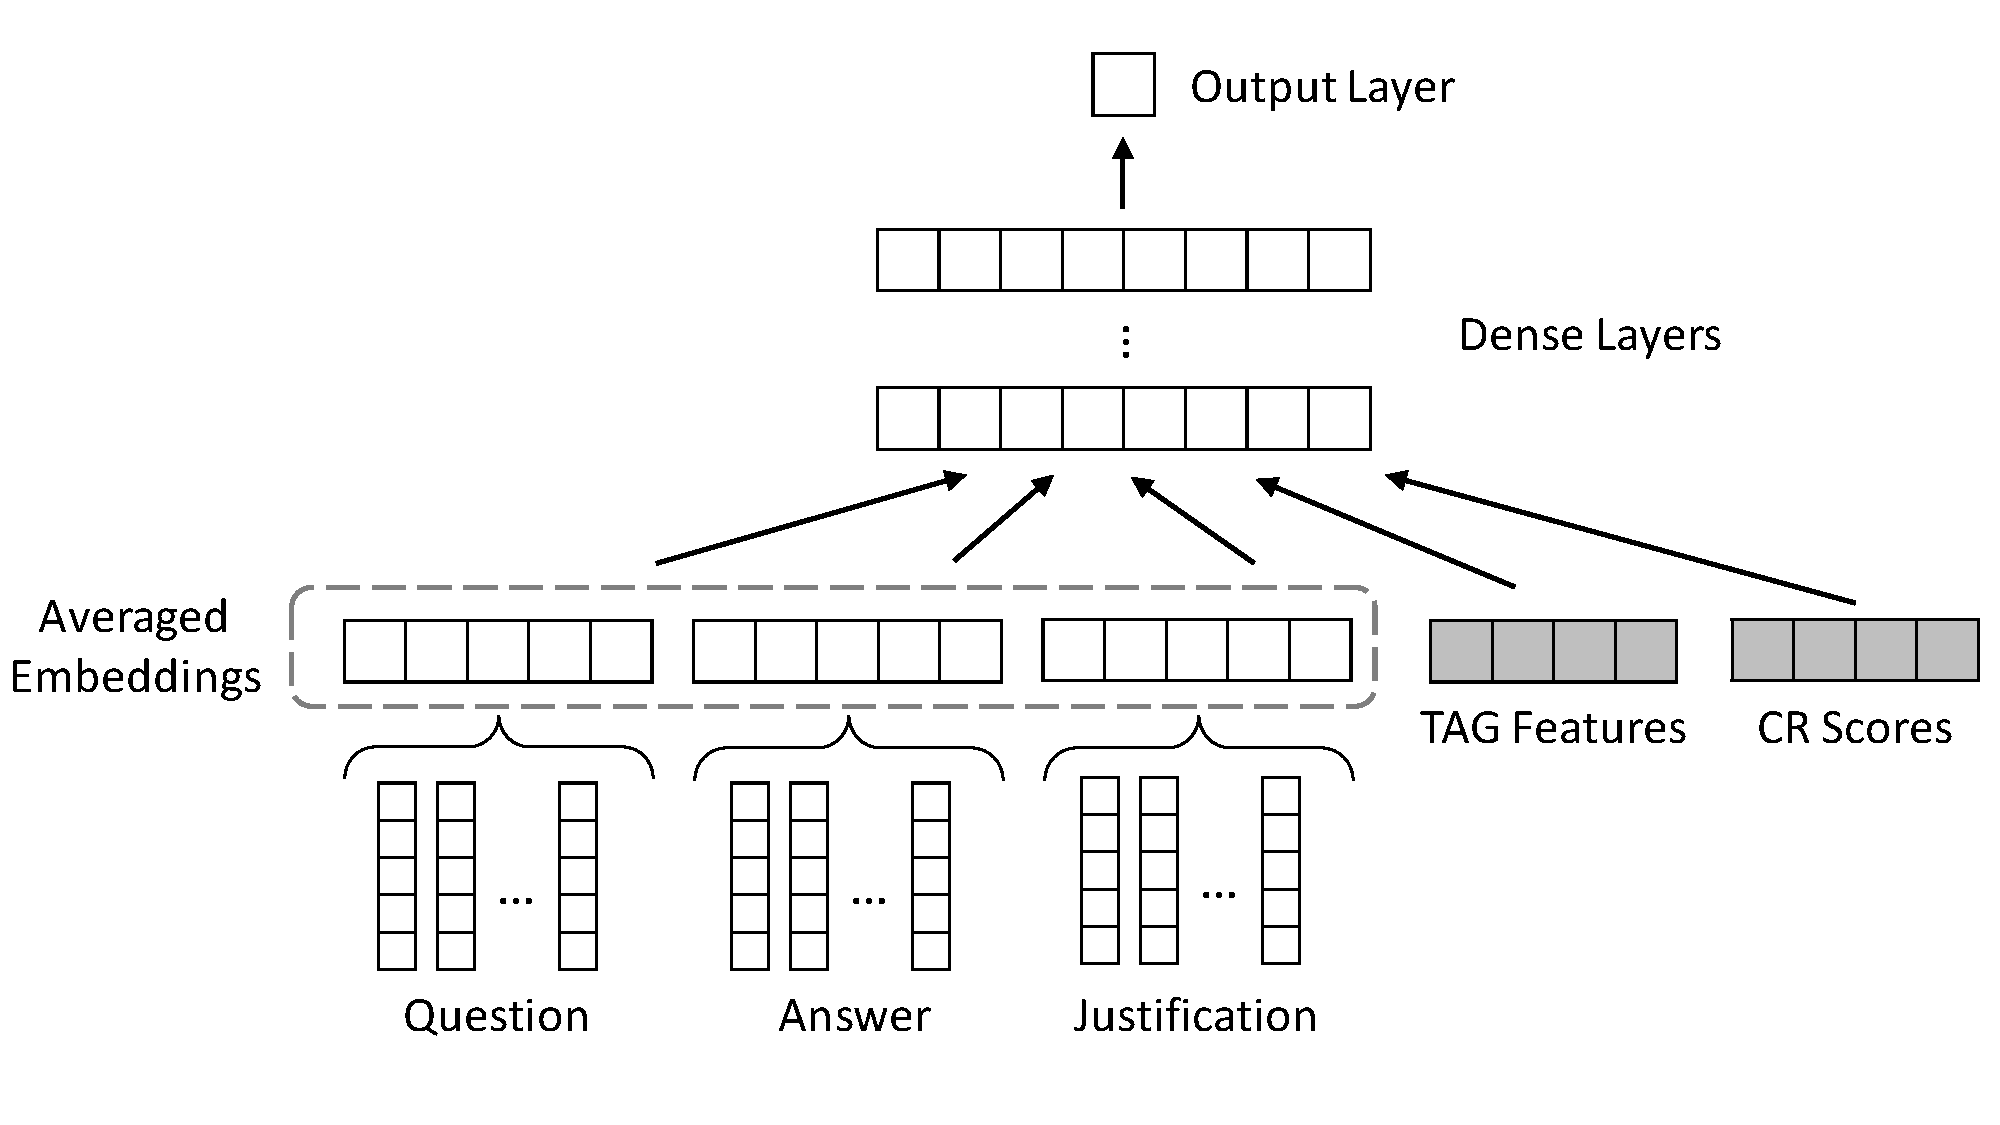
\includegraphics[width=0.8\textwidth]{mainmatter/tacl2015-tig/tagNNArch2scores.pdf}
\caption{The architecture for the neural network variation of our TAG system. We use a fully-connected feed-forward network which takes as input the content words (i.e., nouns, verbs, and adjectives) from the question, candidate answer, and corresponding justification.  For each of these, we create a composite vector by averaging the embeddings of the individual words.  We then concatenate these three composite vectors, as well as the TAG features and the IR scores, to form the input layer to the network. The output of the network is a single, real-valued score for the candidate answer justification.}
\label{fig:nn_arch}
\end{figure}


\subsection{From Latent Perceptron to Latent Neural Networks}
\label{sec-cl2017:nn}

Neural networks (NNs) have recently received much attention in many NLP tasks and have been shown to be quite effective in certain question answering tasks~\citep{Iyyer2014,bordes2014question,bordes2015large,Iyyer2015,wang2015long,dong2015question,yih2015semantic,he2016pairwise,suggu2016deep}.  To determine if a deep learning approach would benefit our system, we explored providing our text aggregation graph features and the information retrieval scores to a neural ranking architecture.  Under this framework we were also able to straightforwardly experiment with including vectorized representations (i.e., embeddings) of the question, candidate answer, and corresponding justification, in hopes of accommodating some of the lexical variation in natural language.

Neural network systems have varied dramatically in terms of their primary architecture (i.e., feed-forward, convolutional, recurrent, etc.) as well as their shape (number of hidden layers, number of nodes in a given layer, etc.).  Recently, however, \citet{Iyyer2015} found that in their QA task, a simple network which \emph{averaged} the word embeddings of the questions and the answer candidates outperformed a much more complex tree recurrent NN.  
\citet{chen2016acl} have recently validated this observation in a different QA task.
We based our NN on this simpler system, adapting it to our task by including not only an averaged vector for the question and answer, but also an averaged vector for the answer justification.  Additionally, we include our connection-type aware structural TAG features (cf., Table \ref{tab:features}) and the information retrieval (IR) features in the network input.  The network architecture is shown in Figure \ref{fig:nn_arch}.

For learning, we use the hinge ranking loss function \citep{collobert2011natural} and update using stochastic gradient descent (SGD).  During training, for each question we pair the correct answer candidate with each of the incorrect candidates, creating three pairs.  For each of these pairs, we score both the correct answer candidate and the incorrect answer candidate and then compute the loss:
\begin{equation}
L = \max (0, m - F(q,a_{correct}) + F(q,a_{incorrect}))
\end{equation}
where $F(q,a_{correct})$ is the score of the correct answer candidate, $F(q,a_{incorrect})$ is the score of the incorrect answer candidate, and $m$ is the margin.


There are two important aspects of the proposed architecture:
\begin{enumerate}
\item[a)] The latent layer, i.e., identifying good justifications to use for a given answer, which we implement by modifying SGD to keep track of the latent aspect.  Specifically, to maintain the latent variable aspect of our ranking perceptron in our ranking neural network, we adapt Equation \ref{eq:F} to use a feed-forward pass through the network to determine the score of a given TAG (rather than the inner product of the features and the parameter vector), and continue to use the implementation of $P$ that uses only the TAG with highest score.  In this way, for each pair of candidate answers we have two justifications (one for the correct answer and one for the incorrect), and so perform a model update (i.e., backpropagation) for each.
\item[b)] The combination of embeddings with explicit features that come from the IR system and the TAG features.  This strategy of mixing latent and explicit features has been demonstrated to be successful in other NLP tasks \citep{chen2014fast,suggu2016deep}.
\end{enumerate} 

Despite their advantages, neural networks have many hyperparameters which need to be tuned.  Continuing the inspiration of \citet{Iyyer2015}, we lightly turned the network on development, both in terms of network shape as well as additional parameters.  Doing so, we arrived at a network which has a single dense layer with length 100 followed by the output layer of length one.\footnote{We experimented with some deeper networks and several hidden layer sizes (both larger and smaller).} 
For our word embeddings, we used a recurrent neural network language model \citep[RNNLM;][]{mikolov10,mikolov13} trained over a concatenation of all of our in-domain elementary science resources (i.e., the study guides, flashcards, and dictionaries) to generate embeddings with 200 dimensions.\footnote{We also experimented with using embeddings trained over English Gigaword \citep{graff2003english} since the resource is much larger and would potentially yield more robust word representations.  However, we found that the performance was consistently worse, which we suspect is due to the difference in the domains.}  


All network nodes use the sigmoid activation function, which performed better and was more stable to variations in the hyperparameters than the rectified linear unit activation.  Additionally, we used an L2 regularization of 1.0 and a dynamic learning rate which began at 1.0 and decayed by half each time the performance on validation decreased.  Though we experimented with dropout, there did not not seem to be a consistent improvement, so our final models do not include it.    
We used 50 epochs for training with early stopping if the validation performance decreased and failed to regain its previous best after 10 epochs.  Similar to the perceptron, we found that the network performance varied with the random seed.  To mitigate the effects of this variation, we report scores from an ensemble of five networks, each with a different random seed, where the trained networks each voted for a single answer choice, splitting their vote only in the event of a tie.


\begin{table*}
\small
\begin{center}
\begin{tabular}{p{0.3mm}p{45mm}ll}
%\multicolumn{1}{l}{ } & \multicolumn{1}{l}{ } & \multicolumn{1}{l}{ } & \multicolumn{1}{l}{P@1}  & \multicolumn{1}{l}{MRR} \\

\# & Neural Network Models  & P\@1 & MRR   \\
% IR - 40.74
% IR + CL + embed - 41.82
% IR + embed - 38.1
% IR + CL - 40.52
% CL - 39.72

\hline
1 & IR				&  40.74\%  & 62.56\%  \\
2 & IR + TAG 		&  40.52\%  & 62.48\% 	\\
3 & IR + embeddings		&  38.74\%  & 61.61\%  	\\
4 & IR + TAG + embeddings	&  41.82\%  & 63.11\%	\\
\end{tabular}
\caption{Performance of the Latent Ranking Neural Network models.  Models with \emph{IR} include the information retrieval scores as input, models with \emph{TAG} use the features from the best performing TAG model (1G\textsubscript{CT}+2G\textsubscript{CT}), and models with \emph{embeddings} include an average embedding for each of the question, the answer, and the text from which the justification graphlet was derived.  Significance tests were performed using bootstrap resampling with 10,000 iterations, but none of the differences between the neural network models and the IR baseline were significant.}
\label{tab:nnresults}
\end{center}
\end{table*}

\paragraph{Neural Network Results}
\label{sec-cl2017:nnresults}


The final performance for the neural network variants of our proposed system as well as the IR baseline are shown in Table \ref{tab:nnresults}.  Once again, we observe that the performance of the combined model (IR + TAG + embeddings, line 4) is better than the performance of the IR model by itself (line 1) or IR + embeddings (line 3). However, here this difference is not significant.  This suggests that representing the justification as a simple bag of words with latent feature representations is not as effective as representing them with features derived from the structure of the text aggregation graph, even with the non-linear capabilities of the neural network.

Additionally, we find that the neural network variants perform worse overall than the latent ranking perceptron models and the voting ensemble (cf., Table \ref{tab:combinedmodels}).  This could be due to the fact that the TAG and IR features we are supplying to the neural network are already abstracted many levels from raw text inputs, and so the NN approach benefits less from the non-linearity of the NN.  Another likely reason for the NN performing worse than the perceptron is that neural architectures need larger quantities of training data in order to properly generalize.  Notably, in the recent Allen Institute for Artificial Intelligence Kaggle challenge\footnote{\url{https://www.kaggle.com/c/the-allen-ai-science-challenge}}, a large contest with 170 participating teams, which also required answering multiple choice elementary and middle school science questions, none of the top-performing participants obtained better results with neural networks. The participants' analyses suggested that this is largely due to a lack of training data.  Finally, the space of possible neural network architectures is large, and the network we report here is fairly simple.  While it could be the case that given a more complex architecture (i.e., with a recurrent or convolutional network, optimizers, and learned rather than pre-trained embeddings) we could obtain even higher numbers than those reported here, with complex architectures, issues resulting from the limited training data would likely be worsened. We leave that exploration to future work.

\paragraph{Incorporating Embeddings into the Perceptron}
Though the embedding-based neural architecture (as implemented) was not successful, following a reviewer suggestion we also experimented with adding the precomputed text embeddings as additional features for the latent ranking perceptron.  In this way, the feature vector for each TAG, $\Phi(x)$, contains the original features as well as an averaged embedding for each of the question, answer, and justification texts.  This provides an additional 600 features, as we are using 200-dimensional embedding vectors.  We included these extra features in our best performing single TAG model, the connection-type aware 1G+2G model shown in Table \ref{tab:combinedmodels}, line 5.  The resulting model performed worse (39.36\% P@1 compared to 42.88\% P@1 without the embeddings). 
This shows that, while distributed representations of words have many benefits (including robustness to lexical variation), their incorporation into a learning model is not necessarily trivial, and we leave that study to future work.

\end{comment}
\section{Discussion}
\label{sec-cl2017:discussion}

To further characterize the performance of our QA approach, we address the following questions: 


%%
%% Comparison with TableILP
%%
%\begin{table}[t]
%\caption{{ Comparison with other models }} % 
%\small
%\begin{center}
%\begin{tabular}{lccc}
%%\cline{2-3}
%%\begin{tabular}{p{20mm}cc}
%\hline
%\multicolumn{1}{c}{Model} & \multicolumn{1}{c}{Questions} &\multicolumn{1}{c}{P@1} \\
%\cline{2-3}
%\hline
%CR $\cup$ (1G\textsubscript{CT} + 2G\textsubscript{CT}) $\cup$ 3G\textsubscript{CT} 			 	& 1000		&	44.6\%	\\
%Khashabi et. al (2016)																				& 200 		&	45.6\%	\\
%
%\end{tabular}
%\label{tab:tableilp}
%\end{center}
%\end{table}

{\flushleft {\bf How does performance compare with methods using manually constructed knowledge bases?}} The TAG system automatically aggregates sentences from six free-text corpora first by building graphlets from those sentences using syntactic dependencies, then connecting those graphlets together into multisentence text aggregation graphs that are then used to both answer questions and provide a compelling human-readable justification for the selected answers.  Recently, Khashabi et al. \citeyear{Khashabi2016QuestionAV} demonstrated that graphs for elementary science QA can also be constructed using a semistructured knowledge base of tables.  In this formalism, dozens of themed tables are manually or semi-automatically constructed, each around a particular theme.  A table's theme is encoded in it's columns, i.e., a table for the color of objects contains two rows, one for the object of interest (e.g., ``leaf''), and another for it's color (e.g., ``green''), while separate instances (e.g., leaf -- green, trunk -- brown) are encoded as different rows.  Each table has between two and five columns.  

The TableILP algorithm answers questions by chaining facts between different table rows, starting from a row that contains question terms, then traversing to a new table row that contains some lexical overlap with the previous row(s), until answer terms are found.  The TAG and TableILP systems are conceptually similar, with the central differences being: (1) The TableILP table row is roughly equivalent to a TAG graphlet with flat structure, and limited to 2--5 information nuggets containing only single terms, (2) TAG graphlets are read automatically from free text corpora, where TableILP tables are largely manually constructed, with methods to automate this construction being actively developed, and (3) the traversal algorithms are different, with TableILP graph building being modelled as an integer linear programming (ILP) problem which finds paths that maximize QA performance.  

The TableILP system reported by Khashabi et al. \citeyear{Khashabi2016QuestionAV} contains 69 tables containing a total of 7,600 rows, with 64 of these tables (approximately 5,000 rows) designed around material in the study guides and a development corpus, and the remaining 2,600 rows distributed amoung 4 automatically constructed tables.  On a corpus of 200 questions drawn from the 1,000 questions used here, TableILP achieved a score of 45.6\% P@1\footnote{We wish to thank Khashabi et al. \citeyear{Khashabi2016QuestionAV} for providing us with this performance figure.}, compared to the 44.6\% P@1 from the best-performing TAG model in Table~\ref{tab:combinedmodels}. The performance difference between these systems is likely not statistically significant.\footnote{We did not have access to system output. However, in our experiments on this dataset, we observed that only differences in P@1 scores of 3\% or higher (absolute) tend to be statistically significant at $p < 0.05$.}

We view these systems as complementary, converging, and with each capable of exploring different aspects of graph-based inference for science QA.  While the TAG focuses on automatically building graphs from free text, this is currently a challenging and noisy process, and as we have shown in Table~\ref{tab:pathlength} and Fried et al.~\citeyear{fried2015higher}, highly susceptable to inference drift as the amount of information required to be aggregated becomes large.  On the other hand, building graphs from manually constructed knowledge bases allow us to investigate the graph-building process in isolation, reducing inference drift due to noise, and further moving this area forward.  

%
% Performance by grade level
%
\begin{table}[t]
\caption{{ Precision@1 by grade level. }} % 
\small
\begin{center}
\begin{tabular}{lccc}
%\cline{2-3}
%\begin{tabular}{p{20mm}cc}
\hline
\multicolumn{1}{c}{Grade Level} & \multicolumn{1}{c}{Questions} &\multicolumn{1}{c}{CR} & \multicolumn{1}{c}{TAG}  \\
\cline{2-3}
\hline
Grade 3 	& 60		&	28.3\%		& 49.2\%	\\
Grade 4		& 69 	&	50.7\%		& 41.3\%	\\
Grade 5		& 871	&	40.2\%		& 42.6\%	\\

\end{tabular}
\label{tab:gradelevel}
\end{center}
\end{table}


{\flushleft {\bf How does performance vary by grade level?}} The question corpus contains third, fourth, and fifth grade questions.  A human with a level of knowledge equivalent to a fourth grade science student might be expected to show better performance for the simpler third grade questions, and decreasing performance as question difficulty increases from fourth to fifth grades.  Table~\ref{tab:gradelevel} shows P@1 performance by grade level for both the CR and best performing TAG model (1G\textsubscript{CT} + 2G\textsubscript{CT}).  The TAG model shows decreasing performance as question difficulty increases, dropping from 49\% for third grade questions to 42\% for fourth and fifth grade questions.  The CR baseline, however, displays a qualitatively different pattern, with a peak performance of 51\% for fourth grade questions, and {\em near chance} performance for third grade questions. 
We believe that observing such a pattern in performance may suggest that the TAG model is a closer approximation of human inference than the baseline based solely on information retrieval.  Here, the relatively small number of third and fourth grade questions prevents us from drawing any conclusions, but suggests that crafting question sets to allow evaluating the distribution of performance by grade level may provide a further measure of comparison between human and machine performance. 



%
% Justification performance by knowledge resource
%
\begin{table}[t]
\caption{{ Most useful knowledge resources for justifications classified as "good".}}
\small
\begin{center}
\begin{tabular}{lccc}
%\cline{2-3}
%\begin{tabular}{p{20mm}cc}
\hline
\multicolumn{1}{l}{Resource} & \multicolumn{1}{c}{Sentences} &\multicolumn{1}{c}{CR} & \multicolumn{1}{c}{TAG}  \\
\cline{2-3}
\hline
Barrons SG 			& 1,200		&	39.3\%		& 43.0\%	\\
Flashcards			& 283		&	16.2\%		& 8.2\%	\\
Teacher's Guide		& 302		&	7.1\%		& 7.0\%	\\
Virginia SG			& 1,314		&	9.1\%		& 9.2\%	\\
Science Dictionary	& 733		&	20.8\%		& 17.8\%	\\
Simple Wiktionary	& 17,473		&	7.5\%		& 14.8\%	\\

\end{tabular}

\label{tab:justificationknowledgeresources}
\end{center}
\end{table}

{\flushleft {\bf Which knowledge resources are generating the most useful answer justifications?}} Shown in Table~\ref{tab:justificationknowledgeresources}, the Barron's Study Guide (SG) contributes more of the \emph{good} justification sentences than any other source, followed by the science dictionary, then the other resources.  Interestingly, the Simple Wicktionary contributes the fewest sentences to the \emph{good} justifications for the CR system (7.5\%), but for the TAG system it is the third largest contributor (14.8\%).  That is, while the CR system is typically unable to find a \emph{good} justification from the Wiktionary, likely owing to it's general nature, the TAG system is able to successfully aggregate these sentences with sentences from other domain-specific sources to build complete justifications.

The vast majority of the \emph{good} justifications generated by the TAG system are aggregates from non-adjacent text: 67\% of the justifications aggregate sentences from \emph{different} corpora, 30\% aggregate non-adjacent sentences within a \emph{single} corpus, while only 3\% of \emph{good} justifications contain sentences that were adjacent in their original corpus. 
This is clear evidence that information aggregation (or fusion) is fundamental for answer justification.


{\flushleft {\bf How orthogonal is the performance of the TAG model when compared to CR?}} Both the TAG and CR models use the same knowledge resources, which on the surface suggests the models may be similar, answering many of the same questions correctly.  The voting models in Table~\ref{tab:combinedmodels} appear to support this, where combining the TAG and CR models increases performance by just under 2\% P@1 over the best-performing TAG model.  To investigate this, we conducted an orthogonality analysis to determine the number of questions both models answer correctly, and the number of questions each model uniquely answers correctly.

Comparing the TAG (1G\textsubscript{CT} + 2G\textsubscript{CT}) and CR models, nearly half of questions are answered correctly by one model and incorrectly by the other.  When combined into a two-way voting model, this causes a large number of ties -- which, resolved at chance, would perform at 42\%, with ceiling performance (i.e., all ties resolved correctly) at 60\%.  This indicates that while the TAG and CR models share about half of their performance, each model is sensitive to different kinds of questions, suggesting that further combination strategies between TAG and CR are worth exploring.


\section{Error Analysis}
\label{sec-cl2017:erroranalysis}

%
% Connection Types in Correct vs Incorrect Answers
%
\begin{table}[t]
\small
\label{tab:errorconnectiontypes}
\begin{center}
%\begin{footnotesize}
%\begin{tabular}{lcc}
%\cline{2-3}
\begin{tabular}{ccc}
\hline
\multicolumn{1}{l}{Connecting Categories} & \multicolumn{1}{c}{Correct} & \multicolumn{1}{c}{Incorrect}  \\
\cline{2-3}
\hline
1				&	31.0\%		& 57.6\%	\\
2				&	56.3\%		& 39.4\%	\\
3				&	12.7\%		& 3.0\%	\\
\end{tabular}
%\end{footnotesize}
\caption{{ Proportion of good justifications with a given number of connecting word categories (Q, A, X) for both correct and incorrect answers. (Top 6) }}
\end{center}
\end{table}

At a high-level, our sentence aggregation model can be thought of as a system for building and evaluating answer justifications.  When questions are answered incorrectly, it is unclear whether the system was unable to \emph{build} a good justification for the correct answer, or unable to \emph{detect} a good justification that was successfully built.  To examine this, in addition to evaluating justification quality for correct answers, we also evaluated the top six justifications for 100 questions that the TAG system answered incorrectly.  We investigated the type of TAG patterns in the correct justifications  (from Section \ref{sec-cl2017:characterizing}), as well as the kinds of inference required for questions that were answered incorrectly.  In addition, we conducted a large open-ended error analysis and identified several broad classes of issues that contribute to poor system performance.\footnote{Our current focus word extractor is not yet well suited to complex multisentence questions. While the question corpus as a whole consists of 62\% single-sentence questions, 25\% two-sentence questions, and 14\% questions which are three sentences or longer, we elected to focus on shorter single-sentence questions for this error analysis whenever possible.  As a result, 96\% of the questions analyzed were single-sentence and 4\% were two-sentence.}

{\flushleft {\bf What patterns of lexical overlap do we observe in justification sentences?}}
We begin with an encouraging result. For questions that were answered incorrectly, nearly half (45.1\%) contain at least one \emph{good} justification within the top 6 for the correct answer.  This suggests that the current model is much better at generating and broadly ranking justifications than it is at the final step -- pushing the correct justification from the top 6 to the top position.  This result suggests that the TAG model may benefit from an improved ranking model. For example, while we currently use lexicalization to model TAG structures and quantify the overlap between candidate TAGs and the question, none of the features used by the ranking perceptron are explicitly lexicalized. 
%We explored some neural network variants of our models in Section \ref{sec-cl2017:nn}, which were better able to incorporate lexicalization, but did not see a performance gain.  These models can be extended in future work, however, to see if it is ultimately possible to make use of this lexicalization.


Further, for questions answered correctly, the \emph{good} justifications in the top 6 tend to connect on several of the three lexical overlap categories (i.e., question focus words, answer focus words, other shared non-focus words).  Table \ref{tab:errorconnectiontypes} shows that for questions answered correctly, in 69\% of cases good justifications are connected on 2 or 3 lexical overlap categories.  
Conversely, for questions that are answered incorrectly, the \emph{good} justifications are far more likely to contain sentences that only connect on a single lexical overlap category (57.6\% vs 31.0\% for questions answered correctly). 
This suggests that while less lexically connected answer justifications are not necessarily less numerous or of lower quality, they are much more challenging to detect given our current connectivity-centered features.  That is, the current features are very good at detecting well connected answer justifications, which correlate with good answers, but the features aren't able to directly detect good answer justifications, which is a more challenging theoretical problem.




%
% Knowledge Types
%
\begin{table}[t]
\small
\begin{center}
\begin{tabular}{lccc}

%\cline{2-3}
%\begin{tabular}{p{20mm}cc}
\hline
\multicolumn{1}{c}{} & \multicolumn{1}{c}{Good} &\multicolumn{1}{c}{No Good} & \multicolumn{1}{c}{}  \\
\multicolumn{1}{l}{Inference Type} & \multicolumn{1}{c}{Justification} &\multicolumn{1}{c}{Justification} & \multicolumn{1}{c}{Overall}  \\

%\cline{2-3}
\hline
Retrieval 			& 58\%		&	23\%		& 39\%	\\
General Inference	& 29\%		&	43\%		& 37\%	\\
Model-Based			& 13\%		&	34\%		& 25\%	\\
\hline
\end{tabular}
\caption{{  A summary of the inference type necessary for incorrectly answered questions.  The summary is broken down into three categories: incorrectly answered questions with a good justification in the top six, incorrectly answered questions without a good justification in the top six, as well as the overall proportions across these two conditions. }} 
\label{tab:knowledgetype}
\end{center}
\end{table}

{\flushleft {\bf Is it harder to detect justifications for certain kinds of inference? }}
We predict that questions requiring more challenging kinds of inference as identified by \citet{clark:2013}, like model-based or general inference questions, are likely more difficult for the TAG system to answer than simpler retrieval-based questions. 
Following the criteria described by Clark et al., we classified the 100 questions in the error analysis based on the inference type required to answer them correctly. 
This analysis, shown in Table~\ref{tab:knowledgetype}, suggests that it is much more challenging to detect \emph{good} justifications for questions that contain challenging inference.  Where 58\% of retrieval-based questions contained a \emph{good} justification within the top 6, this decreased to 29\% for questions requiring general inference, and to 13\% for questions requiring complex model-based reasoning.  Taken in conjunction with our analysis of lexical overlap categories, this suggests that good justifications for complex inference may tend to be less lexically connected, and thus more challenging to detect with our current framework. This suggests important avenues for future work.

\subsection{Broader Error Classes}

\begin{table}[!tb]
\small
\begin{center}
\begin{tabular}{lccc}

%\cline{2-3}
%\begin{tabular}{p{20mm}cc}
\hline
\multicolumn{1}{c}{} & \multicolumn{1}{c}{Good} &\multicolumn{1}{c}{No Good} & \multicolumn{1}{c}{}  \\
\multicolumn{1}{l}{Error Class} & \multicolumn{1}{c}{Justification} &\multicolumn{1}{c}{Justification} & \multicolumn{1}{c}{Overall}  \\

%\cline{2-3}
\hline
\textbf{FOCUS WORDS}  	& 		&		& 	\\
%Focus Word - Question - Major Issues 	& 	27\%		&	30\% 	& 	29\%	\\
%Focus Word - Question - Minor Issues 	& 	22\%		&	16\%		& 	19\%	\\
%Focus Word - Answer - Major Issues 		& 	11\%		&	7\%		& 	9\%	\\
%Focus Word - Answer - Minor Issues 		& 	9\%		&	25\%		& 	18\%	\\
Focus Word --- Question 					& 	49\%		&	46\% 	& 	48\%	\\
Focus Word --- Answer 						& 	20\%		&	32\% 	& 	27\%	\\
Focus Word --- Answer Lists 				& 	7\%		&	5\%		& 	6\%	\\
Focus Word --- Compounds/Collocations 		& 	9\%		&	16\%		& 	13\%	\\
%Focus Word - Answer-type words  			& 	2\%		&	5\%		& 	4\%	\\
\hline
\textbf{NOISE IN THE KNOWLEDGE BASE}		& 			&			& 	\\
Excessively Long Sentence (Chosen Ans) 	& 	33\%		&	9\% 		& 	20\%	\\
Excessively Long Sentence (Correct Ans) 	& 	13\%		&	4\% 		& 	8\%	\\
\hline
\textbf{COMPLEX INFERENCE}				& 			&			& 	\\
More Sentences Required 					& 	4\%		&	16\% 	& 	11\%	\\
Causal or Process Reasoning 				& 	27\%		&	30\%		& 	29\%\\
Quantifiers	 							& 	4\%		&	23\% 	& 	15\%	\\
Negation	 								& 	2\%		&	9\% 		& 	6\%	\\
\hline
\textbf{MISCELLANEOUS}					& 			&			& 	\\
Semantic Cluster Matching				& 	16\%		&	5\%		& 	10\%\\
Coverage of Knowledge Bases				& 	4\%		&	36\%		& 	22\%\\
Other									& 	29\%		&	9\%		& 	18\%\\
\hline
\end{tabular}
\caption{{  A summary of the classes of the errors made by the system. On any given question, more than one error may have been made. The summary is broken down into three categories: incorrectly answered questions with a good justification in the top six, incorrectly answered questions without a good justification in the top six, as well as the overall proportions across these two conditions.}} 
\label{tab:errorclasses}
\end{center}
\end{table}

To expand on the above two issues, we conducted a broader, open-ended error analysis, and identified six main error classes made by the system: focus word failures, noise in the knowledge base, complex inference, semantic cluster matching, coverage of the knowledge bases, and other errors.  The distribution of these errors is shown in Table \ref{tab:errorclasses} and detailed below.

% -------------- FW - MAJOR
 
\begin{table}[]
\begin{footnotesize}
\begin{tabularx}{\textwidth}{p{2.5cm}p{10cm}}
\hline
\multicolumn{2}{l}{Focus Words --- Question} \\
\hline
% Question Info
Question 		& What type of simple machine is Bruce using as he opens a twist top bottle of soda? (GR:5) \\
Focus Word(s) 	& (NN\_bruce, 0.22) (VB\_open, 0.22) (NN\_twist, 0.22) (JJ\_top, 0.22) (NN\_bottle, 0.05) (NN\_soda, 0.03) (NN\_machine, 0.02)		     \\
\textbf{Issue}	& The concept the question is testing is embedded in a complex example that the focus word extractor is only partially able to suppress. Here, the most critical word for the inference is \emph{twist}, but some example words (\emph{bruce, open} and \emph{top}) are not suppressed, and receive the same weight as \emph{twist}. \\
 %which should be removed by the focus word extractor along with \emph{bottle} and \emph{soda}.}\\
\hline
\end{tabularx}
\end{footnotesize}
\caption{{  Example of failure to extract appropriate focus words from the question. }} 
\label{ex:majorfw}
\end{table}


{\flushleft {\bf FOCUS WORD ERRORS: }}
Extracting focus words from questions and answers can be difficult, as often these questions are grounded in complex examples.  Moreover, while examples can often be filtered out, sometimes they are necessary to the question. Within the larger category of focus word errors, we subdivided these errors into more specific categories: 

{\flushleft \emph{Question and Answer Focus Words: }}
We considered a question or answer to have focus word issues if either the words selected by the focus word extractor were not critical to the inference, or if the weights did not reflect the relative importance of each word to the inference.  An example of this can be seen in Table~\ref{ex:majorfw}.

{\flushleft \emph{Answer Choice Lists: }}
Candidate answers may not be single choices, but occasionally take the form of lists, as in the question \emph{which of the following organisms are decomposers?} and its correct answer \emph{worms, mushrooms, and insects}.  In these cases each list item for a given answer candidate must be independently verified for correctness, as incorrect lure answers often contain one or more correct list items.  The current system does not handle this type of complex problem solving method. 

{\flushleft \emph{Compounds/Collocations: }}
The current focus word extractor operates at the level of the word, and does not join noun--noun compounds or collocations, such as \emph{simple machine} or \emph{water cycle}.  This causes compounds to be split, with different focus weights assigned to each word.  This also adds noise to the inference process, as (for example) a justification sentence that contains \emph{simple} but not \emph{machine} is less likely to be on context. 
  

{\flushleft {\bf NOISE IN THE KNOWLEDGE BASE:}}
We included nearly all sentences contained in each of the five science-domain corpora.  While most of this is high-quality text, occasionally extremely long sentences are present (e.g., prefacing a chapter with a list of keywords).  These sentences can cause broad topic-level lexical connections between sentences that are only marginally related to each other, and are a source of noise in the justification building process.  



% -------------- LONGER CHAINS
 
\begin{table}[]
\begin{footnotesize}
\begin{tabularx}{\textwidth}{p{2.5cm}p{10cm}}
\hline
\multicolumn{2}{l}{Complex Inference --- More sentences required to construct a complete answer} \\
\hline
% Question Info
Question 		& Which of the following would result in a decrease in the polar bear population in the arctic? (GR:5) \\
Focus Word(s) 	& (JJ\_polar, 0.29) (NN\_population, 0.29) (NN\_arctic, 0.29) (VB\_result, 0.07) (NN\_decrease, 0.04) (NN\_bear, 0.02) \\
\textbf{Issue}	&  Requires additional graphlets, including that \emph{bears} eat \emph{fish}, \emph{eating} an animal makes you a \emph{predator} and it your \emph{prey}, and a decrease in \emph{prey} population also causes a decrease in \emph{predator} population.  Here, with a limited justification length of two sentences, the system is not able to construct a justification that includes all the crucial focus words, and all answer candidates are left with the same general justification fragment that includes the highest-weighted focus words. \\
\hline
% Correct Answer Info
Correct Answer 	&  a decrease in the fish population \\
Focus Word(s) 	&  (NN\_population, 0.80) (NN\_decrease, 0.13) (NN\_fish, 0.07) \\
Justification 	& A polar bear is a big, white bear that lives in the arctic. (Wiktionary)\\
 				& The population of a place is the people or animals that live there.  (Wiktionary)\\
\hline
% Chosen Answer Info
Chosen Answer 	& a decrease in the human population \\
Focus Word(s) 	& (NN\_population, 0.92) (NN\_decrease, 0.08) \\
Justification 	& A polar bear is a big, white bear that lives in the arctic. (Wiktionary)\\
 				& The population of a place is the people or animals that live there.  (Wiktionary)\\
\hline
\end{tabularx}
\end{footnotesize}
\caption{{  Example of a question that needs more than two sentences to answer. }} 
\label{ex:longerchains}
\end{table}

% -------------- CAUSAL REAS.
 
\begin{table}[]
\begin{footnotesize}
\begin{tabularx}{\textwidth}{p{2.5cm}p{10cm}}
\hline
\multicolumn{2}{l}{Complex Inference --- Causal or Process Reasoning} \\
\hline
% Question Info
Question & In the water cycle, which process occurs {\bf after} condensation? (GR:5)  \\
Focus Word(s) & (NN\_condensation, 0.75) (VB\_occur, 0.13) (NN\_water, 0.06) (NN\_cycle, 0.06)\\
\textbf{Issue}		& Requires knowing that the water cycle is a stage-like process that proceeds as follows: \emph{evaporation}, \emph{condensation}, \emph{precipitation}.  The focus word extractor does not currently detect causal or process markers, and as such the focus words for the question do not include \emph{after}. \\ 
\hline
% Correct Answer Info
Correct Answer &  Precipitation \\
%Focus Word(s) &  (NN\_precipitation, 1.00) \\
Justification 	& Condensation, in the water cycle, {\bf this step leads to} precipitation. (Science Dictionary)\\
 				& When the humidity reaches 100 percent it is very likely that some form of precipitation will occur, depending on the temperature. (Barrons SG)\\
\hline
% Chosen Answer Info
Chosen Answer & Evaporation\\
%Focus Word(s) &  (NN\_evaporation, 1.00)\\
Justification 	& When water vapor changes to liquid water it is called condensation. (Barrons SG)\\
 	& Evaporation is defined as the change of water from its liquid phase to its gaseous phase. (Barrons SG)\\
\hline
\end{tabularx}
\end{footnotesize}
\caption{{  Example of a question that requires reasoning over a causal structure or process. }} 
\label{ex:structure}

\end{table}


% -------------- QUANTIFIERS
 
\begin{table}[]
\begin{footnotesize}
\begin{tabularx}{\textwidth}{p{2.5cm}p{10cm}}
\hline
\multicolumn{2}{l}{Complex Inference --- Quantifiers} \\
\hline
%% Question Info
Question 		& Which of the following is a factor that will cause different species to compete {\bf less?} (GR:5)  \\
Focus Word(s) 	& (NN\_species, 0.50) (JJ\_less, 0.17) (VB\_compete, 0.13) (VB\_cause, 0.10) (JJ\_different, 0.07) (NN\_factor, 0.03)\\
\textbf{Issue}			&  Requires connecting the idea that a \emph{large} supply causes \emph{less} competition.  The focus word extractor does not currently detect quantifiers, and as such the focus words for the correct answer do not include \emph{large}. \\
\hline
%% Correct Answer Info
Correct Answer 	&  A {\bf large} supply of resources\\
Focus Word(s) 	&  (NN\_supply, 0.92) (NN\_resource, 0.08)\\
%Justification 	& Individuals in a species may compete with each other for food, mates, space, water, and shelter within their environment. (Barrons SG)\\
% 				&  A place's infrastructure is the basic public works such as roads, electricity \& water supply, and schools, that allow it to function.  (Wiktionary)\\
\hline
%% Chosen Answer Info
Chosen Answer & {\bf Lack} of space \\
Focus Word(s) &  (NN\_space, 0.92) (NN\_lack, 0.08)\\
%Justification 	& The energy from the sun heated the water and caused it to evaporate - change from liquid water to water vapor. (Barrons SG)\\
% 	& Individuals in a species may compete with each other for food, mates, space, water, and shelter within their environment. (Barrons SG)\\
\hline
\end{tabularx}
\end{footnotesize}
\caption{{  Example of a question that requires an understanding of the quantifiers in both the question and the answers. }} 
\label{ex:quantifiers}
\end{table}

% -------------- NEGATION
 
\begin{table}[]
\begin{footnotesize}
\begin{tabularx}{\textwidth}{p{2.5cm}p{10cm}}
\hline
\multicolumn{2}{l}{Complex Inference --- Negation} \\
\hline
% Question Info
Question & Which of the following is an example of a chemical change? (GR:5)  \\
%Focus Word(s) & (JJ\_chemical, 0.92) (NN\_change, 0.08)\\
\textbf{Issue}			&  Requires detecting negation in the graphlets.  The chosen answer justification contains negative evidence against itself. \\
\hline
% Correct Answer Info
Correct Answer &  Milk souring\\
%Focus Word(s) &  (NN\_souring, 0.67) (NN\_milk, 0.33)\\
Justification 	& Examples of chemical properties include the souring of milk and the ability to burn in the presence of oxygen. (Barrons SG)\\
 				& Evidence of a chemical change could be change in temperature, light, heat, or sound given off, or the formation of gasses. (Science Dictionary)\\
\hline
% Chosen Answer Info
Chosen Answer & Ice cream melting\\
%Focus Word(s) &  (NN\_melting, 0.80) (NN\_cream, 0.13) (NN\_ice, 0.07) \\
Justification 	& Melting of ice is a physical change, {\bf not a chemical change}. (Barrons SG)\\
 	& Melting is a process of an object changing from the solid state to the liquid state without a change in temperature. (Wiktionary)\\
\hline
\end{tabularx}
\end{footnotesize}
\caption{{  Example of a question that requires an understanding of negation. }} 
\label{ex:negations}

\end{table}



{\flushleft {\bf COMPLEX INFERENCE:}}
Despite the elementary-level of our question set, some questions require complex inference to be answered correctly (a recent analysis of a very similar elementary science question set indicated that as many as 77\% of questions required a form of complex inference to solve \citep{jansen-EtAl:2016:COLING}).  This may take the form of requiring longer sequences of graphlets to construct a complete answer justification, requiring an understanding of quantifiers or negation, or a complex inference process. 

{\flushleft \emph{More sentences required: }}
In our knowledge base, a sentence tends to capture a single step in some process. While two sentences are often sufficient to construct a good justification for retrieval-based questions, for general inference and model-based reasoning questions, an inference may require more than two steps.  Further, for questions that are grounded in a concrete example, additional graphlets may be needed to elevate the example words to the more general level of the concepts in our knowledge base -- for example, elevating \emph{polar bear} to \emph{predator} or \emph{animal}, in Table~\ref{ex:longerchains}. 

{\flushleft \emph{Causal or Process Reasoning: }} 
Questions that require causal or process reasoning often require a small structured and ordered representation of that process.  For example, in Table~\ref{ex:structure}, a knowledge of the sequential nature of the water cycle -- that \emph{evaporation} leads to \emph{condensation}, and that \emph{condensation} leads to \emph{precipitation} -- is necessary to answer the question. 

{\flushleft \emph{Quantifiers: }} Some questions require an understanding of quantifiers or scope to arrive at a correct answer, whether these quantifiers are included in the question, answer, or knowledge base.  As illustrated in Table~\ref{ex:quantifiers}, our current system does not implement a knowledge of quantifiers, nor their relationship to each other (e.g., \emph{some} is less than \emph{most}, \emph{smaller} is less than \emph{big}, etc.). 

{\flushleft \emph{Negation: }} Our current framework does not implement a knowledge of negation.  Within the scope of elementary science exams, where questions tend to ask for positive rather than negative evidence, this is often not an issue, with the overall prevalence of questions requiring negation at 6\%.  However, our knowledge bases do include many negated sentences or phrases that provide a contrast between two categories of items through negation (e.g., \emph{melting is a physical change, not a chemical change}). As can be seen in Table~\ref{ex:negations}, these sentences can be misused by our system. 


% -------------- CLUSTER MATCHING
 
\begin{table}[]
\begin{footnotesize}
\begin{tabularx}{\textwidth}{p{2.5cm}p{10cm}}
\hline
\multicolumn{2}{l}{Semantic Cluster Matching} \\
\hline
% Question Info
Question & Which is an example of water condensing? (GR:4)   \\
Focus Word(s) &  (NN\_condensing, 0.92) (NN\_water, 0.08) \\
\textbf{Issue}		& Requires connecting \emph{condensing} in the question with \emph{condensation} in the correct answer justification, based on their high degree of semantic relatedness. \\
\hline
% Correct Answer Info
Correct Answer &  Dew forming on plants during a cold night \\
Focus Word(s) &  (JJ\_cold, 0.68) (NN\_dew, 0.16) (NN\_night, 0.11) (NN\_plant, 0.05) \\
Justification 	& Clouds, dew, water droplets on the outside of a glass on a hot day, are all caused by {\bf condensation}. (Virginia Flash Cards) \\
 				& Think back to a hot summer day, when you poured yourself a glass of cold water and took it outside.  (Barrons SG) \\
\hline
% Chosen Answer Info
Chosen Answer & A puddle disappearing on a hot summer afternoon \\
Focus Word(s) &  (NN\_summer, 0.41) (NN\_afternoon, 0.41) (JJ\_hot, 0.09) (VB\_disappear, 0.06) (NN\_puddle, 0.03) \\
Justification 	& After a few hours or days those puddles disappear. (Barrons SG) \\
			 	& Think back to a hot summer day, when you poured yourself a glass of cold water and took it outside.  (Barrons SG) \\
\hline
\end{tabularx}
\end{footnotesize}
\caption{{  Example of a failure to recognize relatedness or equivalence of words. }} 
\label{ex:clustermatching}

\end{table}


{\flushleft {\bf MISCELLANEOUS:}}

{\flushleft \emph{Semantic Cluster Matching: }}
While the current system reduces noise by making lexical connections only between words in sentences that have the same lemma and part of speech, this strict criterion prevents some \emph{good} justifications from being built, and others from being recognized as \emph{good} justifications.  Ideally, semantically-related terms such as \emph{condensation} and \emph{condensing} (as in Table~\ref{ex:clustermatching}), or \emph{heredity} and \emph{inherit}, could be clustered together to facilitate building more robust answer justifications independent of lexical choice. 

{\flushleft \emph{Coverage of Knowledge Bases: }}
Inevitably our knowledge base suffers from a degree of sparsity, where some topics or specific concepts included in questions are not discussed in any of our corpora.  This rarely happens with grade-appropriate science topics (but does occur for topics such as \emph{competition}).  Coverage issues are much more frequent with the concrete examples that ground the questions, though we  mitigate this by including the simple Wiktionary as a grade-appropriate general knowledge resource.

{\flushleft \emph{Other: }}
While we were able to determine the source for the majority of errors, for 18\% of incorrect questions we were unable to readily identify the issue.  Due to the difficulty of this QA task, we hypothesize that many of these cases may result from the limitations of learning complex latent variables with our learning framework and limited training data. 



\subsection{Summary of Errors}

%space{1mm}
To summarize, this error analysis suggests that a majority of errors are caused by surface issues, and not fundamental limitations of this approach to question answering for science exams.  Were we to solve these issues, including including focus-word extraction errors, noise in the knowledge base, knowledge coverage, and semantic cluster matching, our analysis suggests that 50.5\% of questions answered incorrectly could then be answered correctly.  Using this figure, the ceiling performance for the current model is estimated to be 71.4\%. 

The remainder of errors center on difficulties with complex questions, including questions requiring a knowledge of causality or processes to answer, longer inference chains, or a knowledge of quantifiers or negation.  We hypothesize that many of these questions can be addressed by extending the current model towards including more structure, and making better use of the existing structure within graphlets.  For example, much of the structure within a sentence that explicitly conveys causal or process information (e.g., \emph{from a solid to a liquid}) is not explicitly labelled within a graphlet, or used in a targeted way towards addressing questions that require these kinds of complex inference.  By extending our general methods of justification construction and evaluation to address the specific information needs of these complex questions, we believe that the ceiling performance can be increased considerably, limited only by questions that require complex domain-specific mechanisms, such as spatial reasoning, to answer.  The tradeoff between generality versus domain specificity appears intimately coupled with a model's performance, and other QA systems such as IBM Watson approach QA by assembling a large ensemble of domain-specific models tailored to a given problem representation. 
To surpass the ceiling we observe in our error analysis, one would likely also have to adopt this approach, and implemented dedicated domain-specific methods for the difficult problems left unsolved by our approach. 






%--------------------------------
%  		UNUSED EXAMPLE TABLES
% -------------------------------


% -------------- FW - Minor
 
%\begin{table}[]
%\caption{{  Examples of minor failures to extract appropriate focus words from either the question or answer. }} 
%\begin{footnotesize}
%\begin{tabularx}{\textwidth}{p{2.5cm}p{11cm}}
%\hline
%\multicolumn{2}{l}{EXAMPLE: Focus Word - Question - Minor Issues} \\
%\hline
%% Question Info
%Question & When gasoline and oxygen mix together in a car engine, what happens to the energy in the system? (GR:5)   \\
%Focus Word(s) & (NN\_gasoline, 0.21) (NN\_oxygen, 0.21) (NN\_mix, 0.19) (NN\_energy, 0.19) (NN\_system, 0.06) (RB\_together, 0.05) (NN\_engine, 0.04) (NN\_car, 0.03) (VB\_happen, 0.01)\\
%\textbf{Issue}			&  While the most important words in the question have the highest weight, here the focus word extractor was unable to remove the extraneous question words (e.g. \emph{car, system,} and \emph{together}). \\
%\hline
%% Correct Answer Info
%Correct Answer & It is transferred to motion and heat.\\
%Focus Word(s) & (NN\_motion, 0.34) (NN\_heat, 0.34) (VB\_transfer, 0.31)\\
%Justification 	& Heat energy can be transferred from one object to another object. (Barrons SG)\\
% 				& Generator is a machine that converts mechanical energy (energy in motion) to electrical energy. (Science Dictionary)\\
%\hline
%% Chosen Answer Info
%Chosen Answer & It is transferred to motion and light.\\
%Focus Word(s) & (NN\_motion, 0.34) (NN\_light, 0.34) (VB\_transfer, 0.31)\\
%Justification 	& When you turn on your television, electrical energy is transferred into sound and light energy. (Barrons SG)\\
% 				& The major topics developed in this strand include magnetism, types of motion, simple and compound machines, and energy forms and transformations, especially electricity, sound, and light. (Virginia Framework)\\
%\hline
%\hline
%
%% Answer FW Example 
%\multicolumn{2}{l}{EXAMPLE: Focus Word - Answer - Minor Issues} \\
%\hline
%% Question Info
%Question & Which of the following is the best example of a chemical reaction that produces light, sound, and heat energy? (GR:5)  \\
%Focus Word(s) & (NN\_light, 0.20) (NN\_sound, 0.20) (NN\_energy, 0.20) (VB\_produce, 0.18) (NN\_heat, 0.18) (NN\_chemical, 0.02) (NN\_reaction, 0.02)\\
%\textbf{Issue}			& The answer focus word \emph{firework} received too low a weight for it to be useful. \\
%\hline
%
%% Chosen Answer Info
%Correct Answer & A fireworks display in the sky\\
%Focus Word(s) & (VB\_display, 0.80) (NN\_sky, 0.13) (NN\_firework, 0.07)\\
%Justification 	& Evidence of a chemical change could be change in temperature, light, heat, or sound given off, or the formation of gasses. (Science Dictionary)\\
% 				& Plasma also can be produced in fluorescent lights and plasma display televisions. (Science Dictionary)\\
%\hline
%
%% Chosen Answer Info
%Chosen Answer & Turning on an electric blanket\\
%Focus Word(s) & (VB\_turn, 0.48) (JJ\_electric, 0.48) (NN\_blanket, 0.04)\\
%Justification 	& When you turn on your television, electrical energy is transferred into sound and light energy. (Barrons SG)\\
% 				& Chemical energy changes to electric energy in a battery. (Barrons SG)\\
%\hline
%
%\end{tabularx}
%\end{footnotesize}
%\label{ex:minorfw}
%
%\end{table}

% -------------- FW - A LISTS
 
%\begin{table}[!htb]
%\caption{{  Example of a failure to correctly handle lists in the answer choices. }} 
%\begin{footnotesize}
%\begin{tabularx}{\textwidth}{p{2.5cm}p{11cm}}
%\hline
%\multicolumn{2}{l}{EXAMPLE: /todo{Answer - Lists}} \\
%\hline
%% Question Info
%Question & Which of the following organisms are decomposers? (GR:5)  \\
%Focus Word(s) & (NN\_decomposer, 0.67) (NN\_organism, 0.33)\\
%\textbf{Issue}			& While the focus word extractor currently detects lists, we haven't implemented a problem solving pattern that tries to independently find each element in that list.  \\
%\hline
%% Correct Answer Info
%Correct Answer & Worms, mushrooms, and insects\\
%Focus Word(s) & (NN\_worm, 0.33) (NN\_mushroom, 0.33) (NN\_insect, 0.33)\\
%Justification 	& Decomposer is an organism that breaks down dead animals and decaying matter into other substances. (Science Dictionary)\\
% 				& A creepy-crawly is a small animal that crawls, such as an insect, spider, or worm; this word describes the way these animals move.  (Wiktionary)\\
%\hline
%% Chosen Answer Info
%Chosen Answer & Fish, birds, and animals\\
%Focus Word(s) & (NN\_fish, 0.33) (NN\_bird, 0.33) (NN\_animal, 0.33)\\
%Justification 	& Decomposer is an organism that breaks down dead animals and decaying matter into other substances. (Science Dictionary)\\
% 				& A stuffed animal is a furry toy that is filled with a smooth, white textile substance looking like cotton, the plush. (Wiktionary)\\
%\hline
%
%\end{tabularx}
%\end{footnotesize}
%\label{ex:lists}
%
%\end{table}

%% -------------- FW - COMPOUNDS
% 
%\begin{table}[!htb]
%\caption{{  Example of a failure to recognize and incorporate compounds and collocations  \note{Remove?}}} 
%\begin{footnotesize}
%\begin{tabularx}{\textwidth}{p{2.5cm}p{10cm}}
%\hline
%\multicolumn{2}{l}{EXAMPLE: Focus Word - Compounds/Collocations} \\
%\hline
%% Question Info
%Question & The purpose of simple machines is to \_\_\_. (GR:5) \\
%Focus Word(s) & (NN\_machine, 0.80) (JJ\_simple, 0.13) (NN\_purpose, 0.07)\\
%\textbf{Issue}			&  Here, by not recognizing \emph{simple machine} as a compound, the top justification for the correct answer is very much off-context.\\
%\hline
%% Correct Answer Info
%Correct Answer & decrease the amount of force needed to do work\\
%Focus Word(s) & (NN\_force, 0.41) (VB\_work, 0.41) (NN\_amount, 0.09) (VB\_decrease, 0.06) (VB\_need, 0.03)\\
%Justification 	& Your body is like a very delicate machine that needs to be cared for to work and feel its best. (Barrons SG)\\
% 				& Newton (N) is equal to the amount of force needed to accelerate a mass of one kilogram at a rate of one meter per second per second. (Wiktionary)\\
%\hline
%% Chosen Answer Info
%Chosen Answer & increase the energy used to move objects\\
%Focus Word(s) & (NN\_energy, 0.48) (VB\_move, 0.48) (VB\_increase, 0.04)\\
%Justification 	& Simple Machine is a device without moving parts that is used to make work easier. (Science Dictionary)\\
% 				& A turbine is a machine that uses the kinetic energy of a constant stream of liquid to move a shaft. (Wiktionary)\\
%\hline
%
%\end{tabularx}
%\end{footnotesize}
%\label{ex:compounds}
%
%\end{table}

% -------------- FW - ATYPE
 
%%% PETER'S NOTE: Shouldn't answer-type words only be from the question?  Why is it finding an answer type word in an answer?  
 
%\begin{table}[!htb]
%\caption{{  Example of an inappropriate suppression of words in the answer considered to be </emph answer-type} words. }} 
%\begin{tabularx}{\textwidth}{p{2.5cm}p{11cm}}
%\hline
%\multicolumn{2}{l}{EXAMPLE: Focus Word - Answer-type words} \\
%\hline
%% Question Info
%Question & Air pollution in the city can be reduced by \_\_\_. (GR:5)  \\
%Focus Word(s) & (NN\_air, 0.44) (NN\_pollution, 0.44) (NN\_city, 0.07) (VB\_reduce, 0.04)\\
%\textbf{Issue}			&  In the correct answer, since \emph{vehicle} is considered to be an {\emph answer-type} word, the system does not apply enough weight and so the justification drifts off-context.\\
%\hline
%% Correct Answer Info
%Correct Answer &  limiting the number of vehicles that drive into the city\\
%Focus Word(s) & (NN\_number, 0.41) (VB\_drive, 0.41) (NN\_city, 0.09) (VB\_limit, 0.06) (NN\_vehicle, 0.03)\\
%Justification 	& has more food for organisms, but the organisms usually have to deal with large temperature and salinity changes, high silt content and pollution. (Virginia SG)\\
% 				& The weather in a place is the air temperature, the number of clouds, and the amount of wind and rain or snow.  (Wiktionary)\\
%\hline
%% Chosen Answer Info
%Chosen Answer & limiting the number of people who ride buses and subways\\
%Focus Word(s) &  (NN\_bus, 0.25) (NN\_subway, 0.25) (NN\_number, 0.23) (VB\_ride, 0.23) (VB\_limit, 0.04) (NN\_people, 0.02)\\
%Justification 	& The weather in a place is the air temperature, the number of clouds, and the amount of wind and rain or snow.  (Wiktionary)\\
% 				& A bus is a vehicle that carries a large number of people on roads. (Wiktionary)\\
%\hline
%
%\end{tabularx}
%\label{ex:atype}
%
%\end{table}

% -------------- TOO LONG GRAPHLET
 
%\begin{table}[]
%\caption{{  Example of a question where the inclusion of excessively long graphlets contributed to semantic drift. }} 
%\begin{footnotesize}
%\begin{tabularx}{\textwidth}{p{2.5cm}p{11cm}}
%\hline
%\multicolumn{2}{l}{EXAMPLE: Excessively Long Graphlet} \\
%\hline
%% Question Info
%Question & Which property of air does a barometer measure? (GR:5) \\
%Focus Word(s) & (NN\_measure, 0.75) (NN\_barometer, 0.13) (NN\_property, 0.06) (NN\_air, 0.06)\\
%\textbf{Issue}		& Here, both the correct and chosen answers have noisy graphlets, which allowed the system to make numerous poor connections.\\
%\hline
%% Correct Answer Info
%Correct Answer &  pressure\\
%Focus Word(s) &  (NN\_pressure, 1.00)\\
%Justification 	& Relative humidity is a measure of the amount of water vapor in the air compared to the total amount of water that the air can hold at that temperature. (Virginia SG)\\
% 				& Key concepts include a) weather measurements and meteorological tools (air pressure  barometer, wind speed  anemometer, rainfall  rain gauge, and temperature  thermometer); and b) weather phenomena (fronts, clouds, and storms). (Virginia Framework)\\
%\hline
%% Chosen Answer Info
%Chosen Answer & humidity\\
%Focus Word(s) &  (NN\_humidity, 1.00)\\
%Justification 	& Relative humidity is a measure of the amount of water vapor in the air compared to the total amount of water that the air can hold at that temperature. (Virginia SG)\\
% 	& Standard 4.1 The student will plan and conduct investigations in which a) distinctions are made among observations, conclusions, inferences, and predictions; b) hypotheses are formulated based on cause-and-effect relationships; c) variables that must be held constant in an experimental situation are defined; d) appropriate instruments are selected to measure linear distance, volume, mass, and temperature; e) appropriate metric measures are used to collect, record, and report data; f) data are displayed using bar and basic line graphs; g) numerical data that are contradictory or unusual in experimental results are recognized; and h) predictions are made based on data from picture graphs, bar graphs, and basic line graphs. (Virginia Framework)\\
%\hline
%\end{tabularx}
%\end{footnotesize}
%\label{ex:toolonggraphlet}
%
%\end{table}


 
% -------------- COVERAGE
 
%\begin{table}[]
%\caption{{  Example of a lack of topic coverage in our knowledge bases. \todo{Another example} }} 
%\begin{footnotesize}
%\begin{tabularx}{\textwidth}{p{2.5cm}p{10cm}}
%\hline
%\multicolumn{2}{l}{Coverage of Knowledge Bases} \\
%\hline
%% Question Info
%Question & Which of the following is an example of a chemical change? (GR:5)    \\
%Focus Word(s) &  (JJ\_chemical, 0.92) (NN\_change, 0.08) \\
%\textbf{Issue} 		& Our knowledge bases don't contain information about what happens to an egg when it boils, resulting in our inability to assemble a good justification for the correct answer. \\
%\hline
%% Correct Answer Info
%Correct Answer &  Boiling an egg \\
%Focus Word(s) &  (VB\_boil, 0.92) (NN\_egg, 0.08) \\
%Justification 	& Evidence of a chemical change could be change in temperature, light, heat, or sound given off, or the formation of gasses.  (Science Dictionary)\\
% 				& Boil is to get to a temperature that a liquid lets out bubbles and gas at. (Wiktionary)\\
%\hline
%% Chosen Answer Info
%Chosen Answer & Breaking an egg \\
%Focus Word(s) &  (VB\_break, 0.92) (NN\_egg, 0.08) \\
%Justification 	& Sedimentary rock can form from particles of rock, from remains of plants or animals, or from chemical reactions are classified by their composition and by the way they were formed are formed from the cementing together of small pieces of rocks or shells are called sedimentary rocks are usually found near water are found in flat layers or strata. (Virginia SG)\\
% 	& Physical change examples: Water melting or freezing, crumpling a piece of paper, liquid evaporating, breaking glass (Science Dictionary)\\
%\hline
%\end{tabularx}
%\end{footnotesize}
%\label{ex:coverage}
%
%\end{table}

% -------------- OTHER

%\begin{table}[]
%\caption{{  Example of a questions for which the reason for error is not apparent. }} 
%\begin{tabularx}{\textwidth}{p{2.5cm}p{11cm}}
%\hline
%\multicolumn{2}{l}{EXAMPLE: Other} \\
%\hline
%% Question Info
%Question & Which of the following is an example of a form of energy? (GR:5)  \\
%Focus Word(s) &  (NN\_energy, 1.00) \\
%\textbf{Issue}		&	It is not clear why the system chose the incorrect answer. \\
%\hline
%% Correct Answer Info
%Correct Answer &  the sound in a loud classroom \\
%Focus Word(s) &  (NN\_sound, 0.48) (JJ\_loud, 0.48) (NN\_classroom, 0.04) \\
%Justification 	& Sound is energy (noise) that we hear when matter vibrates and the particles in the matter hit each other. (Barrons SG)\\
% 				& If something thumps, it hits something else, making a loud, low sound. (Wiktionary)\\
%\hline
%% Chosen Answer Info
%Chosen Answer & the water in a small puddle (GR:5)  \\
%Focus Word(s) &  (NN\_puddle, 0.67) (NN\_water, 0.33) \\
%Justification 	& Evaporation is the process in the water cycle in which water from the oceans and lakes is heated up enough by the sun to turn into water vapor in the atmosphere. (Science Dictionary)\\
% 	& The energy from the sun heated the water and caused it to evaporate - change from liquid water to water vapor. (Barrons SG)\\
%\hline
%\end{tabularx}
%\label{ex:other}
%
%\end{table}


%\FloatBarrier		% Prevent the References from getting interspersed with the Tables





\section{Conclusion}
\label{sec-cl2017:conclusion}

We have proposed an approach for QA that emphasizes model interpretability, such that producing human-readable justifications for answers, and evaluating answer justification quality, is the critical component\footnote{To increase reproducibility, all the code behind this effort is released as open-source software\footnote{\url{https://github.com/clulab/releases/tree/master/cl2017-qa}}, which allows other researchers to use our entire science QA system as is, or to explore adapting the various components to other tasks. }.
Our interdisciplinary approach to building and evaluating answer justifications includes cognitively-inspired aspects, such as making use of psycholinguistic concreteness norms for focus word extraction, and making use of age-appropriate knowledge bases, which together help move our approach towards approximating the qualities of human inference on the task of question answering for science exams. Intuitively, our structured representations for answer justifications can be interpreted as a robust approximation of more formal representations, such as logic forms~\citep{moldovan2001logic}. However, to maintain robustness, our approach does not evaluate the quality of connections in these structures by their ability to complete a logic proof, but through a reranking model that measures their correlations with good answers.

In our quest for explainability, we have designed a system that generates answer justifications by chaining sentences together. Our experiments showed that this approach improves explain quality, and, at the same time, answers questions out of reach of information retrieval systems, or systems that process contiguous text.  
We evaluated our approach on 1,000 multiple-choice questions from elementary school science exams, and experimentally demonstrated that our method outperforms several strong baselines at both selecting correct answers, and producing compelling human-readable justifications for those answers.  We further validated our three critical contributions: (a) modeling the high-level task of determining justification quality by using a latent variable model is important for identifying both correct answers and good justifications, (b) identifying focus words using psycholinguistic concreteness norms similarly benefits QA for elementary science exams, and (c) modeling the syntactic and lexical structure of answer justifications allows good justifications to be assembled and detected. 

%We performed a detailed error analysis that suggests several important directions for future work. 
%First, though the majority of errors can be addressed within the proposed formalism and by improving focus word extraction, 47.5\% of incorrectly answered questions would also benefit from more complex inference mechanisms, ranging from causal and process reasoning, to modeling quantifiers and negation.
%This suggests that our robust approach for answer justification may complement deep reasoning methods for QA in the scientific domain~\citep{baral2011towards}.
%Second, while our answer justifications are currently short, future justifications might be quite long, and aggregate sentences from knowledge bases of different domains and genres.  In these situations, combining our procedure for constructing justifications with methods that improve text coherence~\citep{barzilay2008modeling} would likely improve the overall user experience for reading and making use of answer justifications from automated QA systems. 
%Finally, our text aggregation graphs currently capture intersentence connections solely through lexical overlap. We hypothesize that extending these structures to capture lexical-semantic overlap driven by word embeddings~\citep{mikolov13}, which have been demonstrated to be beneficial for QA~\citep{yih13,jansen14,fried2015higher}, would also be beneficial here, and increase robustness on small knowledge bases, where exact lexical matching is often not possible.

Our approach seeks to balance robustness with interpretability by utilizing our lightly-structured graphlets for creating answer justifications.  While here we demonstrate the success of this approach in this domain, performing this structured sentence decomposition and aggregation over larger corpora can become quite cumbersome.  For this reason, in Chapter \ref{chapter:emnlp2017} we propose another model which is designed to be even more robust without losing interpretability.  That is, we explore a similar model which continues to rank answer justifications (maintaining interpretability), but which does not perform aggregation and which makes use of only the shallower free-text representations of the knowledge base sentences and accordingly uses a shallower set of explicit feature (rather than those based on focus words and graphlet structure, increasing robustness).  %Additionally, we increase the power of the learning framework by moving from a linear perceptron to a non-linear neural network.



%\newpage
%\starttwocolumn
%\bibliographystyle{fullname}
%\bibliography{refs}


% Our packages
%\usepackage{float}
%\usepackage[font=small]{caption}
%\usepackage{color}
%\usepackage{graphicx}
%\usepackage{booktabs}
%\usepackage{subcaption}
%\usepackage{hyperref}
%\usepackage[utf8]{inputenc}
%\usepackage{tabularx}
%\usepackage{tablefootnote}
%\usepackage{amsmath}
%\usepackage{amssymb}
%\usepackage{placeins}
%\usepackage{scrextend}

%\title{Tell Me Why: Using Question Answering as Distant Supervision for Answer Justification}


%\begin{abstract}
%
%For many applications of question answering (QA), being able to explain why a given model chose an answer is critical.  However, the lack of labeled data for  answer justifications makes learning this difficult and expensive.  Here we propose an approach that uses answer ranking as distant supervision for learning how to select informative justifications. 
%We propose a neural network architecture for QA that reranks answer justifications as an intermediate (and human-interpretable) step in answer selection. Our approach is informed by a set of features designed to combine both learned representations and explicit features to capture the connection between questions, answers, and answer justifications.
% We show that with this end-to-end approach we are able to significantly improve upon a strong IR baseline in both justification ranking (+9\% rated highly relevant) and answer selection (+6\% P@1).  %We also provide an error analysis that demonstrates that we can use the justifications returned to better understand what our model has learned.
%\end{abstract}

\chapter{EMNLP2017 - QAJ\label{chapter:emnlp2017}}

%\section{Introduction}
\label{sec-emnlp2017:intro}
%
%Developing interpretable machine learning (ML) models, that is, models where a human user can \emph{understand} what the model is learning, is considered by many to be crucial for ensuring usability and accelerating progress \cite{craven1996extracting,Kim2015MindTG, letham2015interpretable, Ribeiro2016WhySI}.  
%% bs: removed for space, we talk more about this in related work
%%As such, it has received much attention in recent years, especially as deep learning and complex architectures have seen dramatic gains in many tasks.
%For many applications of question answering (QA), i.e., finding short answers to natural language questions, simply providing an answer is not sufficient. A complete approach must be interpretable, i.e., able to {\em explain} why an answer is correct. 
%For example, in the medical domain, a QA approach that answers treatment questions would not be trusted if the treatment recommendation is not explained in terms that can be understood by the human user. 
%
%
%One approach to interpreting complex models is to make use of human-interpretable information % metric % ms: not a metric...
% generated by the model to gain insight into what the model is learning.  This can be an intermediate representation used by the model, as with the model-generated text spans of \citet{Lei2016RationalizingNP}, that serve as input to another classification network.  
%By learning these intermediate representations end-to-end with a downstream task, they are optimized to correlate with what the model learns is discriminatory for the task, and they can be evaluated against what a human would consider to be important.
%\todo{need to define what a downstream task means to use this term}, they are optimized to correlate with what the model learns is discriminatory for the task, and they can be evaluated against what a human would consider to be important.
%Here we apply this general framework for model interpretability to QA.
%
%
%\begin{table}[t]
%\begin{center}
%\begin{footnotesize}
%\begin{tabularx}{\linewidth}{p{0.13cm}p{6.8cm}}
%\multicolumn{2}{p{8cm}}{\textbf{Question:} Which of these is a response to an internal stimulus?} \\
% (A) & A sunflower turns to face the rising sun. \\
% (B) & A cucumber tendril wraps around a wire. \\
% (C) &  A pine tree knocked sideways in a landslide grows upward in a bend. \\
% (\textbf{D}) &\textbf{Guard cells of a tomato plant leaf close when there is little water in the roots .} \\
%\\
%\multicolumn{2}{p{7.2cm}}{\textbf{Justification:} 
%Plants rely on hormones to send signals within the plant in order to respond to internal stimuli such as a lack of water or nutrients. } \\
%
%\end{tabularx}
%\end{footnotesize}
%\caption{{  Example of an 8th grade science question with a justification for the correct answer.  Note the lack of direct lexical overlap present between the justification and the correct answer, demonstrating the difficulty of the task of finding justifications using traditional distant supervision methods. }}
%%space{-6mm} 
%\label{tab:question_example}
%\end{center}
%\end{table}
%
%In this work, we focus on answering multiple-choice science exam questions (Clark \citeyear{clark:2015}; see example in Table~\ref{tab:question_example}). 
%This domain is challenging as: (a) approximately 70\% of science exam question shave been shown to require complex forms of inference to solve \cite{clark:2013,jansen-EtAl:2016:COLING}, and (b) there are few structured knowledge bases to support this inference.  
%Within this domain, we propose an approach that learns to both select and explain answers, when the only supervision available is for which answer is correct (but not how to explain it).
%Intuitively, our approach chooses the justifications that provide the most help towards ranking the correct answers higher than incorrect ones.
%More formally, our neural network approach alternates between using the current model with max-pooling to choose the highest scoring justifications for correct answers, and optimizing the answer ranking model given these justifications. 
%Crucially, these reranked texts serve as our human-readable answer justifications, and by examining them, we gain insight into what the model learned was useful for the QA task.   


The specific contributions of this work are:
\begin{enumerate}
\item We propose an end-to-end neural method for learning to answer questions and select a high-quality justification for those answers. 
Our approach re-ranks free-text answer justifications without the need for structured knowledge bases. 
With supervision only for the correct answers, we learn this re-ranking through a form of distant supervision -- i.e., the answer ranking supervises the justification re-ranking. 

\item We investigate two distinct categories of features in this ``little data'' domain: explicit features, and learned representations. We show that, with limited training, explicit features perform far better despite their simplicity. 

\item We demonstrate a large (+9\%) improvement in generating high-quality justifications over a strong information retrieval (IR) baseline, while maintaining near state-of-the-art performance on the multiple-choice science-exam QA task, demonstrating the success of the end-to-end strategy.
\end{enumerate}

%\section{Related work}

In many ways, deep learning has become the canonical example of the "black box" of machine learning and many of the approaches to explaining it can be loosely categorized into two types: approaches that try to interpret the parameters themselves (e.g., with visualizations and heat maps \citep{Zeiler2014VisualizingAU,nips15_hermann, Li2016VisualizingAU}, and approaches that generate a human-interpretable metric that is ideally correlated with what is being learned inside the model (e.g., \citet{Lei2016RationalizingNP}). Our approach falls into the latter type -- 
we use our model's reranking of human-readable justifications to give us insight into what the model considers informative for answering questions.  This allows us to see where we do well (Section \ref{sec-emnlp2017:justification_results}), and where we can improve (Section  \ref{sec-emnlp2017:erroranalysis}).

Deep learning has been successfully applied to many recent QA approaches and related tasks \cite[][inter alia]{Bordes2015LargescaleSQ,nips15_hermann, He2016CharacterLevelQA, dong2015question, Tan2016ImprovedRL}.
%are enticing, and for good reason -- many recent approaches to question answering and related tasks have had much success with various deep learning models \cite[][inter alia]{Bordes2015LargescaleSQ,nips15_hermann, He2016CharacterLevelQA, dong2015question, Tan2016ImprovedRL}.  
However, large quantities of data are needed to train the millions of parameters often contained in these models.  
%Of potentially greater utility in low-data domains, 
Recently, simpler model architectures have been proposed that greatly reduce the number of parameters while maintaining high performance \cite[e.g.,][]{Iyyer2015,chen2016thorough,Parikh2016ADA}.  
%For example, \citet{Iyyer2015}'s show that with their Deep Averaged Network, which replaces complex recurrent neural networks with an average of embeddings and a few, albeit large, dense layers, they improved performance on both a sentiment analysis and a QA task.  For natural language inference, \citet{Parikh2016ADA} used a simpler neural alignment  approach with an attention mechanisms to greatly reduce the size of their model while reaching then state-of-the-art performance.  
We take inspiration from this trend and propose a simple neural architecture for our task to offset the limited available training data. 

Another way to mitigate sparse training data is to include higher-level explicit features.  Like \citet{sachan2016science}, we make use of explicit features alongside features from distributed representations to capture connections between questions, answers, and supporting text.  However, we use a simpler set of features and while they use structured and semi-structured knowledge bases, we use only free-text.  %Additionally, though we also learn to select support from our knowledge base (in some ways similar to \citeauthor{sachan2016science}'s latent answer-entailing structure), since we are explicitly trying to perform \emph{explainable} question answering, here we evaluate the justifications learned by our approach and show that they are significantly better than a  strong IR baseline (Section \ref{sec-emnlp2017:justification_results}).   

Our approach to learning justification reranking end-to-end with answer selection is similar to the \citet{jansen2017framing} latent reranking perceptron,  which also operates over free text.  However, our approach does not require decomposing the text into an intermediate representation, allowing our technique to more easily extend to larger textual knowledge bases.  
%ir approach is able to aggregate information from a variety of sources into one justification, our light-weight approach however, does not rely on a large set of heuristics and heavy pre-processing to transform free-text into a structured knowledge base.  

The way we have formulated our justification selection (as a re-ranking of knowledge base sentences) is related to, but distinct from the task of answer sentence selection \cite[][inter alia]{Wang2010ProbabilisticTM, Severyn:12,Severyn:13a,Severyn:13b,Severyn2015LearningTR,wang2015long}.  Answer sentence selection is typically framed as a fully or semi-supervised task for factoid questions, where a correctly selected sentence fully contains the answer text.
%and the problem is designed such that a correctly selected sentence will fully contain the answer text.
Here, we have a variety of questions, many of which are non-factoid.  Additionally, we have no direct supervision for our justification selection (i.e., no labels as to which sentences are good justifications for our answers), motivating our distant supervision approach where the performance on our QA task serves as supervision for selecting good justifications.  Further, we are not actually looking for sentences that \emph{contain} the answer choice, as with answer sentence selection, but rather sentences which close the "lexical chasm" \cite{Berger:00} between question and answer (demonstrated in the example in Table \ref{tab:question_example}). 


%Related work: QA, multiple choice, kaggle challenge, explanation-centered inference, model-specific work (NNs, etc)

%Latest QA papers (latest trends, attn, etc)
%Inspired by this literature (cite DAN \& SNLI, simpler better), but we add this latent layer they don’t have (justification quality). For simple archs: see Danqi Chen at ACL 2016 (similar to DAN but for reading comprehension). 

%Attention models (ACL 2016). Simple especially when you don’t have enough data.

%(visualizations vs analysis of embeddings VS correlated metric EMNLP paper, etc -- interpreting wts if DL is impossible, rather, find correlations betw those and explanatory natural language)

 
%\todo{Add a paragraph comparing against the task of answer sentence selection (see that reviewer from CL, and all those kernel-based papers by Moschitti). The difference is that in our case the answer and its justification arrive from different sources (i.e., the answer is provided in the multiple-choice exam, whereas the justification is extracted from study guides), whereas in previous answer sentence selection work the answer is included in the sentence. In our case we have to deal with bigger ``lexical chasm'' between question/answer/justification.}

%\todo{Discriminative information retrieval for question answering sentence selection(Chen and Van-Durme): Presented a method that selects sentences which contain potential answers for questions from a very large corpus (10\^7 sentences, requiring several thousand questions for training). Their results are dramatically better than Lucene across two datasets and several evaluation measures.}
%(Yih et al.,2013; Wang and Manning, 2010; Heilman and Smith, 2010; Yao et al., 2013a) and recently using neural networks (Yu et al., 2014; Severyn and Moschitti,2015; Wang and Nyberg, 2015; Yin et al.,2016)

%Answer sentence selection diff because we don't need (or want?) complete answer inclusion.

%Our sentences being selected are unlabeled.

%TAG paper!!! 
%\section{Neural justification reranking}
%\label{sec-emnlp2017:intro}

Once again, we are concerned with developing interpretable models for question answering.  In Chapter \ref{chapter:cl2017} we proposed a method for question answering that created and ranked human-readable answer justifications using performance on the QA task as the only form of supervision.  We demonstrated that not only did it outperform a strong information retrieval baseline in terms of correctly answering questions, but it also produced a higher percentage of good justifications, as rated by human annotators. The main drawback to the system was simply in the somewhat heavy cost of the sentence processing.  While this processing was able to be done offline (and so only once), the time and size burden still prevents its practical use over extremely large corpora. 

Here, we propose an approach that once again uses answer ranking as distant supervision for learning how to select informative justifications.  As with the previous approach, our justifications serve as inferential connections between the question and the correct answer while often containing little lexical overlap with either.  However, here in this  modified approach we use a  shallower representation of knowledge base sentences and we do not perform aggregation, facilitating usage over much larger resources.  
We additionally extend the linear learning framework used in Chapter \ref{chapter:cl2017} through the use of deep learning (specifically, a non-linear feed-forward neural network), as described in Section \ref{sec-emnlp2017:approach}.  
In making these modifications to increase the robustness of the approach, we purposefully maintain our interpretability -- we continue to rank and return human-readable answer justifications for our model's chosen answers.

\section{Chapter Outline}
The remainder of the chapter is organized as follows.  First, we review related work in Section \ref{sec-emnlp2017:relatedwork}.  In Section \ref{sec-emnlp2017:approach} we describe our overall neural approach for QA that reranks answer justifications as an intermediate (and human-interpretable) step in answer selection. In Section \ref{sec-emnlp2017:pipeline} we describe our neural network in more detail.  In that same section, we also describe our set of features designed to combine both learned representations (i.e. embeddings) and explicit features to capture the connection between questions, answers, and answer justifications.  Then, in Section \ref{sec-emnlp2017:experiments} we provide the details of our experimental setup and in Section \ref{sec-emnlp2017:results} we provide our reseults -- with this end-to-end approach we are able to significantly improve upon a strong IR baseline in both justification ranking (+9\% rated highly relevant) and answer selection (+6\% P@1).  In Section \ref{sec-emnlp2017:erroranalysis} we utilize our model-returned justifications in an error analysis.  Finally, in Section \ref{sec-emnlp2017:conclusions} are our conclusions.



\section{Related Work}
\label{sec-emnlp2017:relatedwork}
In many ways, deep learning has become the canonical example of the "black box" of machine learning and many of the approaches to explaining it can be loosely categorized into two types: approaches that try to interpret the parameters themselves (e.g., with visualizations and heat maps \citep{Zeiler2014VisualizingAU,nips15_hermann, Li2016VisualizingAU}, and approaches that generate human-interpretable information that is ideally correlated with what is being learned inside the model (e.g., \citet{Lei2016RationalizingNP}). Our approach falls into the latter type -- 
we use our model's reranking of human-readable justifications to give us insight into what the model considers informative for answering questions.  This allows us to see where we do well (Section \ref{sec-emnlp2017:justification_results}), and where we can improve (Section  \ref{sec-emnlp2017:erroranalysis}).

Deep learning has been successfully applied to many recent QA approaches and related tasks \citep[][inter alia]{Bordes2015LargescaleSQ,nips15_hermann, He2016CharacterLevelQA, dong2015question, Tan2016ImprovedRL}.
However, large quantities of data are needed to train the millions of parameters often contained in these models.  
Recently, simpler model architectures have been proposed that greatly reduce the number of parameters while maintaining high performance \cite[e.g.,][]{Iyyer2015,chen2016thorough,Parikh2016ADA}.  
%For example, \citet{Iyyer2015}'s show that with their Deep Averaged Network, which replaces complex recurrent neural networks with an average of embeddings and a few, albeit large, dense layers, they improved performance on both a sentiment analysis and a QA task.  For natural language inference, \citet{Parikh2016ADA} used a simpler neural alignment approach with an attention mechanism to greatly reduce the size of their model while reaching then state-of-the-art performance.  
We take inspiration from this trend and propose a simple neural architecture for our task to offset the limited available training data. 


Another way to mitigate sparse training data is to include higher-level explicit features.  Like \citet{sachan2016science}, we make use of explicit features alongside features from distributed representations (see Section \ref{sec-emnlp2017:features}) to capture connections between questions, answers, and supporting text.  However, we use a simpler set of features and while they use structured and semi-structured knowledge bases, we use only free-text.  %Additionally, though we also learn to select support from our knowledge base (in some ways similar to \citeauthor{sachan2016science}'s latent answer-entailing structure), since we are explicitly trying to perform \emph{explainable} question answering, here we evaluate the justifications learned by our approach and show that they are significantly better than a  strong IR baseline (Section \ref{sec:justification_results}).   

%Our approach to learning justification reranking end-to-end with answer selection is similar to the \citet[][described in Chapter \ref{chapter:cl2017}]{jansen2017framing} latent reranking perceptron,  which also operates over free text.  However, our approach does not require decomposing the text into an intermediate representation, allowing our technique to more easily extend to larger textual knowledge bases.  


%\todo{Discriminative information retrieval for question answering sentence selection(Chen and Van-Durme): Presented a method that selects sentences which contain potential answers for questions from a very large corpus (10\^7 sentences, requiring several thousand questions for training). Their results are dramatically better than Lucene across two datasets and several evaluation measures.}
%(Yih et al.,2013; Wang and Manning, 2010; Heilman and Smith, 2010; Yao et al., 2013a) and recently using neural networks (Yu et al., 2014; Severyn and Moschitti,2015; Wang and Nyberg, 2015; Yin et al.,2016)


\begin{figure}[t]
\begin{center}
\includegraphics[width=0.5\textwidth]{mainmatter/emnlp2017-qaj/arch_overall.png}
\caption{ Architecture of our question answering approach.  
Given a question, candidate answer, and a free-text knowledge base as inputs, we generate a pool of candidate justifications, from which we extract feature vectors.  We use a neural network to score each and then retain \textit{only} the highest-scoring justification from the pool of candidates (i.e., max-pooling), thus selecting the current best justification. This justification score serves as the score for the candidate answer itself.  The red border indicates the components that are trained online. }
\label{fig:arch_overall}
%space{-5mm}
\end{center}
\end{figure}

\section{Approach}
\label{sec-emnlp2017:approach}
One of the primary difficulties with the explainable QA task addressed here is that, while we have supervision for the correct answer, we do not have annotated answer justifications.  
Here we tackle this challenge by using the QA task performance as supervision for the justification reranking, allowing us to 
%extending a neural QA model to jointly learn both how to 
%jointly 
learn to choose both the correct answer and a compelling, human-readable justification for that answer.

Additionally, similar to the strategy \citet{chen2014fast} applied to parsing, we combine representation-based features with explicit features that capture additional information that is difficult to model through embeddings, especially with limited training data.


% ms: avoid "system" too engineering-y
The architecture of our approach is summarized in Figure \ref{fig:arch_overall}.  
Given a question and a candidate answer, we first query an textual knowledge base (KB) to retrieve a pool of potential justifications for that answer candidate.  
For each justification, we extract a set of features designed to model the relations between questions, answers, and answer justifications based on word embeddings, lexical overlap with the question and answer candidate, discourse, and information retrieval (IR) (Section \ref{sec-emnlp2017:features}).
These features are passed into a simple neural network to generate a score for each justification, given the current state of the model.  A final max-pooling layer filters the input, retaining only the top-scoring justification for the candidate answer and this max score is used also as the score for the answer candidate.  In relation to the latent variable perceptron proposed in Section \ref{sec-cl2017:model}, this max-pooling layer is functionally identical to the latent $P$ function that learns to identify the good justifications for a given answer (recall that we implemented $P$ such that it selects exactly one justification at each iteration -- the best-performing, given the current state of the model).
The final candidate answer score (also shown in Figure \ref{fig:arch}) essentially takes the place of $F(q_i, a_j)$ in Equation \ref{eq:F}.     
The system is trained using correct-incorrect answer pairs with a pairwise margin ranking loss objective function to enforce that the correct answer be ranked higher than any of the incorrect answers. 

%The key here is that we use the current state of the model to select the best justification for a given answer candidate from a pool of many candidate justifications.  To do this, we modify the training procedure such that at the start of each epoch \todo{minibatch instead of epoch?}, we first compute a forward pass with each candidate justification to find the top-scoring justification for each candidate answer.
%For a given question, answer candidate, and justification, we combine features based on word embeddings, lexical overlap, discourse, and information retrieval (IR) together in a simple neural architecture to generate a score for the answer candidate.    We then use this selected justification to calculate our gradients for updating the model parameters.  

With this end-to-end approach, the model learns to select justifications that allow it to correctly answer questions.  We hypothesize that, as with the system in Chapter \ref{chapter:cl2017}, this approach enables the model to indirectly learn to choose justifications that provide good explanations as to why the answer is correct. We empirically test this hypothesis in Section \ref{sec-emnlp2017:results}, where we show that
%indeed the model outperforms several strong baselines in both QA performance (correctly answering questions) as well as justification performance (i.e., selecting a justification for an answer that fully explains its connection to the question).
 indeed the model learns to correctly answer questions, as well as to select justifications that fully explain the connection between those answers to the corresponding questions.
% ms: misleading; it reads as if answer selection is better than IR
% better than a strong IR baseline. 


\begin{figure}[t]
\begin{center}
\includegraphics[width=0.8\textwidth]{mainmatter/emnlp2017-qaj/ArchDiagram.png}
\caption{ Detailed architecture of the model's scoring component.  
The question, candidate answer, and justification %\edit{(previously obtained through max-pooling)}
% bs: no - the max pooling happens at the end, after the scoring. 
 are encoded (by summing their word embeddings) to create vector representations of each. These representations are combined in several ways to create a set of representation-based similarity features that are concatenated to additional explicit features capturing lexical overlap, discourse and IR information and fed into a feed-forward neural network.  The output layer of the network is a single node that represents the score of the justification candidate.}  %\todo{Take out? As described in Section \ref{sec-emnlp2017:approach}, we then use max-pooling over these justification scores to assign a score to the answer candidate itself.} }
 %bs: sure -- it's shown in the arch right next door :)
\label{fig:arch}
%space{-5mm}
\end{center}
\end{figure}


\section{Model and Features}
\label{sec-emnlp2017:pipeline}
%\bs{we're low on space and I'm not sure we really need all the features in table 2... in fact, do we need the table at all? \\similarity features are described in prose, as are discourse features (and example is in sep figure), and IR++ features.  Should we remove the table and move the description of LO features to prose? we could recapture half a column...}.  
% removed table per mihai email
Our approach consists of three main components: (a) the retrieval of a pool of candidate answer justifications (Section \ref{sec-emnlp2017:justretrieval}); (b) the extraction of features for each (Section \ref{sec-emnlp2017:features}); and (c) the scoring of the answer candidate itself based on this pool of justifications (Section \ref{sec-emnlp2017:nn_model}).  The architecture of this latter scoring component is shown in Figure \ref{fig:arch}. 


\begin{table}[h!]
\begin{center}
\begin{footnotesize}
\begin{tabular}{p{0.5cm}p{12cm}}
%\hline
%Feature  & Description \\ 
\hline
\multicolumn{2}{l}{Representation-Based Features (Emb)} \\
\hline
\multicolumn{2}{l}{$sim(Q,A)$, $sim(Q,J)$, and $sim(Q,J)$} \\
  & The pairwise cosine similarities between the question, answer, and justification representations. \\
\multicolumn{2}{l}{$sim(Q, uniqueJ)$ and $sim(A, uniqueJ)$} \\
& The cosine similarities between each of the question and answer representations and the representation for the terms in the justification which don't overlap with either. \\
\multicolumn{2}{l}{$dist(Q + J, A)$} \\
 & The euclidean distance between the sum of the question and justification representations and that of the answer (see Section \ref{sec-emnlp2017:features} for motivation and details).\\
\hline
\multicolumn{2}{l}{Lexical Overlap Features (LO)} \\
\hline
\multicolumn{2}{l}{\emph{qCoverage}, \emph{aCoverage}, and \emph{qaCoverage}} \\
 & The proportion of question words, of answer words, and of the combined set of question and answer words that also appear in the justification. \\
% & The proportion of answer words that also appear in the justification. \\
% & The proportion of combined question and answer words that also appear in the justification. \\ 
\multicolumn{2}{l}{\emph{jNovelty}} \\
 & The proportion of justification words that do not appear in either the question or the answer. \\
\multicolumn{2}{l}{\emph{numWords}} \\
 & Length of the justification in words.\tablefootnote{We normalized this value by the maximum justification length.} \\

\hline
\multicolumn{2}{l}{Semi-Lexicalized Discourse Features (lexDisc)} \\
\hline
\multicolumn{2}{l}{\emph{lexDisc$_0$, ..., lexDisc$_n$}} \\
 & A set of indicator-like features that capture the presence of semi-lexicalized discourse relations (see Section \ref{sec-emnlp2017:features} for details and example). \\
 \hline
\multicolumn{2}{l}{IR-Based Features (IR$^{++}$)} \\
\hline
\multicolumn{2}{l}{\emph{IR$_{max}$, IR$_{sum}$}} \\
 & The reciprocal rank of the answer candidate based on (a) the highest scoring IR-retrieved document and (b) the weighted sum of all the IR-retrieved documents, using the basic IR query (see \ref{sec-emnlp2017:features} for details).\\
\multicolumn{2}{l}{\emph{IR$_{max}^{boosted}$, IR$_{sum}^{boosted}$}} \\
 & The reciprocal rank of the answer candidate based on (a) the highest scoring IR-retrieved document and (b) the weighted sum of all the IR-retrieved documents, using the boosted IR query (see \ref{sec-emnlp2017:features} for details). \\

\end{tabular}
\end{footnotesize}
\caption{{ Summary of the features calculated for each candidate justification.  
 }} 
\label{tab:feature_examples}
\end{center}
\end{table}

\subsection{Candidate Justification Retrieval}
\label{sec-emnlp2017:justretrieval}
The first step in our process is to use standard information retrieval (IR) methods to retrieve a set of candidate justifications for each candidate answer to a given question.  To do this, we build a bag-of-words query using the content lemmas for the question and answer candidate, boosting the answer lemmas to have four times more weight\footnote{We empirically found this answer term boosting to ensure retrieval of documents which were relevant to the particular answer candidate.}.  We used Lucene\footnote{\url{https://lucene.apache.org}} with a \emph{tf-idf} based scoring function to return the top-scoring documents from the knowledge base.  Each of these indexed documents consists of a single sentence from our corpora, and serves as one potential justification.  
%\todo{Say here that each Lucene document indexes one potential justification, i.e., one sentence from X, or one paragraph from Y?}

\subsection{Feature Extraction}
\label{sec-emnlp2017:features}
For each retrieved candidate justification, we extract a set of features based on (a) distributed representations (i.e., word embeddings) of the question, candidate answer, and justification terms; (b) strict lexical overlap; (c) discourse relations present in the justification; and (d) the IR scores for the justification.  Each of these features is described in detail below, and a summary is provided in Table \ref{tab:feature_examples}.

{ \flushleft{\bf Representation-based features (Emb):}} To model the similarity between the text of each question ($Q$), candidate answer ($A$), and candidate justification ($J$), i.e. the answer passage from the IR model, we include a set of features that utilize distributed representations of the words found in each.
%\todo{Needs to explain where the justification vector comes from (e.g. answer passage from IR model)} 
%bs: I disagree -- I think it's pretty clear from 4.1 above.  I added "text" above to make it clearer.  sorry - but we have no space!!!
First we encode each 
%we make a single vector representation for each of the question ($Q$), answer candidate ($A$), and justification ($J$) 
by summing the word embedding vectors for each of their words.\footnote{While this bag-of-words approach is not ideal in many ways, it performed equivalently to far more complicated approaches such as LSTMs and GRUs, also noted by \citep{Iyyer2015}, likely due to the limited training data in this domain.}.  We then compute $sim(Q, A)$, $sim(Q, J)$, and $sim(A, J)$ using cosine similarity.  Using another vector representation of only the \emph{unique} words in the justification, i.e., the words that do not occur in either the question or the candidate answer, we also compute $sim(Q, uniqueJ)$ and $sim(A, uniqueJ)$.  

To create a feature which captures the relationship between the question, answer, \emph{and} justification, we take inspiration from TransE, a popular relation extraction framework \citep{Bordes2013TranslatingEF}.  TransE is based on the premise that if two entities, $e_1$ and $e_2$ are related by a relation $r$, then a mapping into $k$ dimensions, $m(x) \in \mathbb{R}^k$ can be learned such that $m(e_1) + m(r) \approx m(e_2)$.  Here, we modify this intuition for QA by suggesting that given the vectorized representations of the question, answer candidate, and justification above, $Q + J \approx A$, i.e., a question combined with a strong justification will point towards an answer.  Here we model this as an explicit feature, the euclidean distance between $Q + J$ and $A$, and hypothesize that as a consequence the model will learn to select passages that maximize the quality of the justifications.
%Thus, we calculate a feature which is the euclidean distance between $Q + J$ and $A$.  Our intuition is that a question combined with a strong justification will point towards an answer.  Here we model this as an explicit feature, and hypothesize that as a consequence the model will learn to select passages that maximize the quality of the justifications.
This makes a total of six features based on distributed representations. %\todo{This is an important theoretical idea, and should be explicitly stated. e.g. (Our intuition is that a question combined with a strong justification will point towards an answer.  Here we model this as an explicit feature, and hypothesize that as a consequence the model will learn to select passages that maximize the quailty of the justifications.)}  

{\flushleft{\bf Lexical overlap features (LO):}} 
%\todo{This is not a great name, because the next features are also explicit... Maybe, lexical overlap features} 
We additionally characterize each justification in terms of a simple set of explicit features designed to capture the size of the justification, as well as the lexical overlap (and difference) between the justification and the question and answer candidate.  We include these five features: the proportion of question words, of answer words, and of the combined set of question and answer words that also appear in the justification; the proportion of justification words that do not appear in either the question or the answer; and the length of the justification in words.\footnote{We normalized this value by the maximum justification length.} 
%The full set of LO features are shown in Table \ref{tab:feature_examples}.


\begin{figure}[t]
\begin{center}
\includegraphics[width=0.8\textwidth]{mainmatter/emnlp2017-qaj/DiscourseExample.png}
\caption{Example showing the discourse feature extracted from a question, answer, and justification.  Words occurring in the question are shown in blue and words occurring in the answer are shown in green.  The boxes around the justification text indicate the elementary discourse units identified by the discourse parser, and the arrow indicates the found discourse relation (with the assigned relation label given in red). }
\label{fig:discourseexample}
\vspace{-5mm}
\end{center}
\end{figure}

{\flushleft{\bf Semi-Lexicalized Discourse features (lexDisc):}}  These features use the discourse structure of the justification text, which has been shown to be useful for QA~\citep[][see also Chapter \ref{chapter:naacl2015}]{jansen14,sharp-EtAl:2015:NAACL-HLT, sachan2016science}. %, to generate a set of explicit discourse features.  

We use the discourse parser of \citet{Surdeanu:15} to first fragment the text into elementary discourse units (EDUs) and then recursively connects neighboring EDUs together, assigning each a binary discourse relation label such as \emph{Elaboration} or \emph{Contrast}. Each of these discourse relations consists of a head, a relation label, and a modifier. 
%which is based on the architecture of \citet{hernault10} and \citet{feng12}.  This parser first parses each justification into its elementary discourse units (EDUs) and then recursively connects neighboring EDUs together, assigning each a binary discourse relation label such as \emph{Elaboration} or \emph{Contrast}. Each of these discourse relations consists of a head, a relation label, and a modifier.  
%
For each of the 18 possible relation labels (listed in Table \todo{make table in naacl paper chapter}), we create 
a set of semi-lexicalized discourse features that indicate the presence of a given discourse relation as well as whether or not the head and modifier texts contain words from the question and/or the answer.  %This is similar to the discourse-based features of \citet{sachan2016science}, which were the concatenation of the question word (i.e., \emph{why} or \emph{how}) to the relation labels of background sentences.   

Consider, for example, the question \emph{Q: What makes water a good solvent...?  A: strong polarity} shown in Figure \ref{fig:discourseexample}.  The discourse parser identified a causal relation in the justifcation:  [{\em Water is an efficient solvent}]$_{e1}$ [{\em because of this polarity.}]$_{e2}$.  From this discourse relation, we create the semi-lexicalized feature \emph{Q}\_\emph{cause}\_\emph{A}, because there is a {\em Cause} relation between EDUs $e1$ and $e2$, $e1$ overlaps lexically with the question (i.e. \textit{water} and \textit{solvent}}, and $e2$ overlaps lexically with the answer (i.e., \textit{polarity}).
%For example, for the justification [{\em Water is an efficient solvent}]$_{e1}$ [{\em because of this polarity.}]$_{e2}$, we create the semi-lexicalized feature \emph{Q\_cause\_A}, because there is a {\em Cause} relation between EDUs $e1$ and $e2$, $e1$ overlaps with the question ({\em What makes water a good solvent...?}), and $e2$ overlaps with the answer ({\em strong polarity}).
Since there are 18 possible discourse relation labels, and the prefix and suffix can be any of \emph{Q, A, QA} or \emph{None}, this creates a set of 288 indicator features\footnote{In practice these features can be greater than 1.0.  We wanted to maintain the indicator-like quality of the features while still capturing if a given justification contains several of a certain type of discourse feature.  Thus, we use the fourth-root of the count of each of the discourse features present in the justification as the feature value.}, though in practice many combinations are never found.


%
%Consider the example in Figure \ref{fig:discourseexample}, where the justification contains a \emph{Cause} relation whose head contains question words (shown in blue) and whose modifier contains answer words (shown in green).  This corresponds to the semi-lexicalized feature \emph{Q\_cause\_A}.  Since there are 18 possible discourse relation labels, and the prefix and suffix can be any of \emph{Q, A, QA} or \emph{None}, this creates a set of 288 indicator features

{\flushleft{\bf IR-based features (IR$^{++}$):}} 
%\todo{rework in consideration of query details above}
Finally, we also use a set of four IR-based features which are assigned at the level of the answer candidate (i.e., these features are identical for each of the candidate justifications for that answer choice).   
%Given a question and answer candidate, we query the IR system with the content lemmas from both.  
Using the same query method as described in Section \ref{sec-emnlp2017:justretrieval}, for each question and answer candidate we retrieve a set of indexed documents.
Using the \emph{tf-idf} based retrieval scores of these returned documents, 
$s(d_i)$ for $d_i \in D$, we rank the answer candidates using two methods: 
\begin{itemize}
\item by the maximum retrieved document score for each candidate, and  
\item by the weighted sum of all retrieved document scores\footnote{Weighted sum was based on the IR scores used in the winning Kaggle system from user Cardal (\scriptsize{ \url{https://github.com/Cardal/Kaggle_AllenAIscience}})}:

\begin{equation}
\sum_{d_i \in D} \dfrac{1}{i} s(d_i) 
\end{equation}

\end{itemize}
We repeat this process using an unboosted query as well, for a total of four rankings of the answer candidates.  
We then use these rankings to make a set of four reciprocal rank features,  IR$^{++}_0$, ..., IR$^{++}_3$, for each answer candidate (i.e., IR$^{++}_0 = 1.0$ for the top-ranked candidate in the first ranking,  IR$^{++}_0 = 0.5$ for the next candidate, etc.)
%For each answer candidate, we use its position in each of the four rankings above to make a reciprocal rank feature -- these are the IR$^{++}$ features. 
  
%For each of these four IR-based rankings of the answer candidates, We transform these four IR-based rankings into a set of four reciprocal rank features for each answer candidate. 


\subsection{Neural Network}
\label{sec-emnlp2017:nn_model}

As shown in Figure \ref{fig:arch}, the extracted features for each candidate justification are concatenated and passed into a fully-connected feed-forward neural network.  The output layer is a single node representing the justification score.  We then use max-pooling over these scores to select the current best justification for the answer candidate, and use its score as the score for the answer candidate itself.  For training, the correct answer for a given question is paired with each of the incorrect answers, and each are scored as above.  We compute the pair-wise margin ranking loss for each training pair:

\begin{equation}
L = \max(0, m - F(a^{+}) + F(a^{-}))
\end{equation}

where $F(a^+)$ and $F(a^-)$ are the model scores for a correct and incorrect answer candidate and $m$ is the margin, and backpropagate the gradients.
At testing time, we use the trained model to score each answer choice (again using the maximum justification score) and select the highest-scoring.

As we are interested in not only correctly answering questions, but also selecting valid justification for those answers, we keep track of the scores of \emph{all} justifications and use this information to return the top $k$ justifications for each answer choice.  These are evaluated along with the answer selection performance in Section \ref{sec-emnlp2017:results}.

\section{Experiments}
\label{sec-emnlp2017:experiments}

\subsection{Data and Setup}
We evaluated our model on the set of 8th grade science questions that was provided by the Allen Institute for Artificial Intelligence (AI2) for a recent Kaggle challenge.  The training set contained 2,500 question, each with 4 answer candidates.  For our test set, we used the 800 publicly-released questions that were used as the validation set in the actual evaluation.\footnote{The official testing dataset is not publicly available.}  We tuned our model architectures and hyper-parameters on the training data using five-fold cross-validation (training on 4 folds, validating on 1).  During testing, we froze the model architecture and all hyperparameters and re-trained on all the training data, setting aside a random 15\% of training questions to facilitate early stopping. 
%That is, \todo{explain how early stopping works.}  
% sorry mihai -- no room adn it's common practice in DL.  that sai, if a reviewer wants to know, I'm more than happy to address it with a 9th page...

\subsection{Baselines}
In addition to previous work, we compare our model against two strong IR baselines:
%\paragraph{IR Baseline:} For this baseline, we rank answer candidates by the maximum \emph{tf.idf} document retrieval score using an unboosted query of question and answer terms (see Section \ref{sec-emnlp2017:justretrieval} for retrieval details).
%
%\paragraph{IR$^{++}$:}  This baseline uses the same architecture as the full model, as described in Section \ref{sec-emnlp2017:nn_model}, but with only the IR$^{++}$ feature group.

\begin{itemize}
\item \textbf{IR Baseline:} For this baseline, we rank answer candidates by the maximum \emph{tf.idf} document retrieval score using an unboosted query of question and answer terms (see Section \ref{sec-emnlp2017:justretrieval} for retrieval details).

\item \textbf{IR$^{++}$:}  This baseline uses the same architecture as the full model, as described in Section \ref{sec-emnlp2017:nn_model}, but with only the IR$^{++}$ feature group.
\end{itemize}

\subsection{Corpora}
For our pool of candidate justifications (as well as the scores for our IR baselines) we used the corpora that were cited as being most helpful to the top-performing systems of the Kaggle challenge.  These consisted of short, flash-card style texts gathered from two online resources:  about 700K sentences from StudyStack\footnote{{\scriptsize \url{https://www.studystack.com/}}} and 25K sentences from Quizlet\footnote{{\scriptsize \url{https://quizlet.com/}}}.
From these corpora, we use the top 50 sentences retrieved by the IR model as our set of candidate justifications.  All of our corpora were annotated using using the Stanford CoreNLP toolkit~\cite{manning2014stanford}, the dependency parser of Chen and Manning~\citeyear{chen2014fast}, and the discourse parser of \citet{Surdeanu:15}.
% and indexed with \todo{lucene}. 
%\todo{Explain what a ``document'' is for these resources.} 
%\bs{I do that now in Sect 4.1 -- is that sufficient?}

While our model is able to learn a set of embeddings, we found performance was improved when using pre-trained embeddings, and in this low-data domain, fixing these embeddings to not update during training substantially reduced the amount of model over-fitting.   In order to pre-train domain-relevant embeddings for our vocabulary, we used the documents from the StudyStack and Quizlet corpora, supplemented by the newly released Aristo \textsc{mini} corpus (December 2016 release)\footnote{{\scriptsize \url{http://allenai.org/}}}, which contains 1.2M science-related sentences from various web sources.  The training was done using the \texttt{word2vec} algorithm \cite{mikolov10, mikolov13} as implemented by \citet{levy2014dependency}, such that the context for each word in a sentence is composed of all the other words in the same sentence.  We used embeddings of size 50 as we did not see a performance improvement with higher dimensionality.

\subsection{Model Tuning}
The neural model was implemented in Keras \cite{chollet2015keras} using the Theano \cite{2016arXiv160502688short} backend.  For our feed-forward component, we use a shallow neural network that we lightly tuned to have a single fully-connected layer containing 10 nodes, glorot uniform initialization, a $tanh$ activation, and an L2-regularization of 0.1.  We trained with the RMSProp optimizer \citep{rmsprop},  a learning rate of 0.001, 100 epochs, a batch size of 32, and early stopping with a patience of 5 epochs.  Our loss function used a margin of 1.0.  

We experimented with burn-in, i.e., using the best justification chosen by the IR model for the first mini-batches, but found that models without burn-in performed better, indicating that the model benefited from being able to select its own justification.
 
\begin{table}[t!]
\begin{center}
\begin{footnotesize}
\begin{tabular}{llll}
\hline
\# & Model & P@1 Val & P@1 Test \\ 
%\hline
%& Baselines & \\
\hline
1	&	Random 			&			25			&  25	\\
2	&	IR Baseline		&			47.2			&	 47	\\
3	&	IR$^{++}$ 		&			50.7$^{**}$			& 36.35	\\
4 & \citet{Iyyer2015}
%\tablefootnote{Our implementation of the architecture described in the paper, using the same embeddings we used with our model and dense layers of equal dimension to our embeddings.} 
& -- & 32.52\\
5 & \citet{khot2017tupleinf} & -- & 46.17 \\
%\hline
%	&	Our Approach & 	&	\\
\hline
6 & Our approach w/o IR	&	50.54$^*$	& 48.66 \\
%7	&	IR$^{++}$ + EF 					&		53.4$^{**\dagger\dagger}$				& 53.4$^{**}$	\\
%8	&	IR$^{++}$ + EF + lexDisc 	&		53.6$^{**\dagger\dagger}$				& 53.42$^{**\dagger}$ 	\\
7	&	Our approach  &	{\bf 54.0}$^{**\dagger\dagger}$		& {\bf 53.3}$^{**\dagger}$ 	\\
\end{tabular}
\end{footnotesize}
%space{-1mm}
\caption{{ Performance on the AI2 Kaggle questions, measured by precision-at-one (P@1).  $^*$s  indicate that the difference between the corresponding model and the IR baseline is statistically significant ($^*$ indicates $p < 0.05$ and $^{**}$ indicates $p < 0.001$) and $^{\dagger}$s  indicate significance compared to IR$^{++}$,
%that the difference between the corresponding model and the IR$^{++}$ baseline is statistically significant. %($^\dagger$ corresponds to $p < 0.05$ and $^{\dagger\dagger}$ corresponds to $p < 0.001$).  
All significance values were determined through a one-tailed bootstrap resampling test with 100,000 iterations. }} 
\label{tab:p@1}
\end{center}
\end{table}

\begin{table}[t!]
\begin{center}
\begin{footnotesize}
\begin{tabular}{ll}
\hline
 Ablated Model & P@1 Val \\ 
\hline
 %LO + lexDisc + Emb	&	50.54$^*$ \\
    %Baseline IR$^{++}$ 							&		50.7$^{**}$	\\
	IR$^{++}$ + LO 					&		53.4$^{**\dagger\dagger}$\\
	IR$^{++}$ + LO + lexDisc 	&		53.6$^{**\dagger\dagger}$ \\
    Full Model (IR$^{++}$ + LO + lexDisc + Emb)  &	{\bf 54.0}$^{**\dagger\dagger}$	\\
\end{tabular}
\end{footnotesize}
%space{-1mm}
\caption{{ Ablation of feature groups results, measured by precision-at-one (P@1) on validation data.  Emb indicates our embedding-based features, LO indicates our lexical overlap features, lexDisc signifies our semi-lexicalized discourse features, and IR$^{++}$ indicates our information retrieval based features.  Significance is indicated as in Table \ref{tab:p@1}.}} 
\label{tab:ablation}
%space{-5mm}
\end{center}
\end{table}

\section{Results}
\label{sec-emnlp2017:results}

Rather than seeking to outperform all other systems at selecting the correct answer to a question, here we aimed to construct a system  that can produce substantially better justifications for why the answer choice is correct to a human user (i.e., that is interpretable), without unduly sacrificing accuracy on the answer selection task (i.e., that maintains robustness).  Accordingly, we evaluate our system both in terms of it's ability to correctly answer questions (Section \ref{sec-emnlp2017:accuracy}), as well as provide high-quality justifications for those answers (\ref{sec-emnlp2017:justification_results}).  Additionally, we perform an error analysis (Section \ref{sec-emnlp2017:erroranalysis}), taking advantage of the insight the reranked justifications provide into what the model is learning.
% \todo{not sure what this sentence means?}.
% bs: is this clearer?

\subsection{QA Performance}
\label{sec-emnlp2017:accuracy}
We evaluated the accuracy of our system as well as the baselines on the held-out 800 set of test questions.  Performance, measured in precision at 1 \citep[P@1;][]{manning08}, is shown in Table \ref{tab:p@1} for both the validation (i.e., cross validation on training) and test partitions.  Because NNs are sensitive to initialization, each experimental result shown is the average performance across five runs, each using different random seeds.   

The best performing baseline on the validation data was a model using only IR$^{++}$ features (line 3), but its performance dropped substantially when evaluated on test due to the failure of several random seed initializations to learn.  For this reason, we assessed significance of our model combinations with respect to both the IR baseline as well as the IR$^{++}$ (indicated by $^*$ and $^{\dagger}$s, respectively). All significance values were determined through a one-tailed bootstrap resampling test with 100,000 iterations (see Section \ref{sec-naacl2015:results}, Footnote \ref{footnote:bootstrap} for implementation).
%For this reason, we assessed significance of our model combinations with respect to both the IR baseline (indicated by $^*$) as well as the IR$^{++}$ system (indicated by $^{\dagger}$s).

Our full model that combines IR$^{++}$, lexical overlap, discourse, and embeddings-based features, has a P@1 of 53.3\% (line 7), an absolute gain of 6.3\% over the strong IR baseline despite using the same background knowledge.  
% + LO + lexDisc + Emb\todo{use the text description to make it easier for the reader, e.g. (that combines IR++ with lexical overlap, ...}, has a P@1 of 53.3, an absolute gain of 6.3\% over the strong IR baseline despite using the same background knowledge.  

%\subsubsection{Comparison to Previous Work}
%\begin{flushleft}
%{\bf Comparison to Previous Work}
%space{-1mm}
%\end{flushleft}
\paragraph{Comparison to Previous Work:}
We compared our performance against another model that achieves state of the art performance on a different set of 8th grade science questions, \textsc{TupleInf}(T+T') \citep{khot2017tupleinf}.  \textsc{TupleInf}(T+T') uses Integer Linear Programming to find support for questions via tuple representations of KB sentences\footnote{Notably, one portion of the tuple KB used was constructed based on a different 8th grade question set than the one we use here.}.
%with structured Open IE \citep{Banko2007OpenIE} tuple representations of both questions and knowledge-base sentences to assess how well a given answer choice is entailed or supported.  
On our test data, \textsc{TupleInf}(T+T') achieves 46.17\% P@1 (line 5). 
%\todo{move back to 1 sigdig?}.  
As this model is independent of an IR component, we compare its performance against our full system without the IR-based features (line 6), whose performance is 48.66\% P@1, an absolute improvement of 2.49\% P@1 (5.4\% relative) despite our unstructured text inputs and the far smaller size of our knowledge base (three orders of magnitude). 

%Notably, their KB used by \citeauthor{khot2017tupleinf} is three orders of magnitude larger than ours.  
%Waterloo -- 280GB, ours is SS+QZ -- 72.5MB

\citet{sachan2016science} also tackle the AI2 Kaggle question set with an approach  that learns alignments between questions and structured and semi-structured KB data.
%They reframe the task as answer entailment and learn alignments between structured and semi-structured KB data and the question-answer hypothesis.  
They use only the training questions (splitting them into training, validation, and testing partitions), supplemented by questions found in online study guides, and report an accuracy of 47.84\%.  By way of a loose comparison (since we are evaluating on different data partitions), our model has approximately 5\% higher performance despite our simpler set of features and unstructured KB.  

We also compare our model to our implementation of the basic Deep-Averaged Network (DAN) Architecture of \citet{Iyyer2015}.  %To ensure a more fair comparison, 
We used the same 50-dimensional embeddings in both models, so with the reduced embedding dimension, we reduced the size of each of the DAN dense layer to 50 as well.  For simplicity, we also did not implement their word-dropout, a feature that they reported as providing a performance boost. Using this implementation, the performance on the test set was 31.50\% P@1.  To help with observed overfitting, we tried removing the dense layers and received a small boost to 32.52\% P@1 (line 4).  
The lower performance of their model, which relies exclusively on latent representations of the data, underscores the benefit of including explicit features alongside latent features in a deep-learning approach for this domain.
%This lower performance demonstrates, again, \todo{change to "The lower performance of their model, which relies on latent representations of the data, underscores the relative importance of including both explicit and latent features in a deep-learning solver"?}. the utility of explicit features alongside latent representations in low-data domains.

In comparison to other systems that competed in the Kaggle challenge, our system comes in in 7th place out of 170 competitors (top 4\%).\footnote{Based on the public leaderboard ({\scriptsize \url{https://www.kaggle.com/c/the-allen-ai-science-challenge/leaderboard}}). The best scoring submission had an accuracy of 59.38\%.  Note that for the systems that participated, this set served as \emph{validation} while for us it was test, and thus it is likely that these scores are slightly overfitted to this dataset, but for us it was blind.  As such this is a conservative comparison, and in reality the difference is likely to be smaller.}  Compared with the systems which disclosed their methods, we use a subset of their corpora and substantially less hyperparameter tuning, and yet we achieve competitive results.  
%\todo{count cardal hyperparameters and add}
%bs - removed hyperparam count todo bc it's not straightforward and we're out of space anyway.
%\todo{add paragraph for DAN}

%\subsection{Feature Ablation}
%\begin{flushleft}
%{\bf Feature Ablation }
%space{-2mm}
%\end{flushleft}

\paragraph{Feature Contribution:} To evaluate the contribution of the individual feature groups, we additionally performed an ablation experiment by removing one feature group at a time and then re-evaluating.  The results of this experiment are shown in Table \ref{tab:ablation}.
Each of our ablated models performed significantly better than the IR baseline on the validation set, including our simplest model that includes only the lexical overlap and IR-based feature, IR$^{++}$+LO\footnote{As we consider the fully ablated IR$^{++}$ to be a baseline, we do not include it here.}.
%, and the version which has the IR-based features removed, LO+lexDisc+Emb.  
   
%The addition of the semi-lexicalized discourse features (lexDisc) did not significantly improve performance over IR$^{++}$+EF, but it did add the stability needed to show significant gains over IR$^{++}$ (compare lines 3 and 5).  
%The addition of the distributional similarity features, which led to our best performing model on the validation data did not improve performance on the test data (line 5), suggesting that while distributional similarity has been shown effective in situations where there is sufficient training data, it struggles to contribute in low-data domains.  Recall that due to over-fitting issues, we fixed our model embeddings, and so while we used domain-specific embeddings, they were not tuned to be task-specific.  We suspect that given more training data we would see much more benefit from these distributional similarity features.


%
% Justification example
%
\begin{table}[t]
\begin{center}
%\begin{footnotesize}
%\begin{tabular}{p{1cm}p(6cm}}
\begin{tabularx}{\linewidth}{p{2cm}p{12cm}}
\hline
\multicolumn{2}{c}{Question} \\
\hline			
\multicolumn{2}{p{14cm}}{\textbf{Q:} Scientists use ice cores to help predict the impact of future atmospheric changes on climate. Which property of ice cores do these scientists use? } \\
\multicolumn{2}{p{15cm}}{\textbf{A:} The composition of ancient materials trapped in air bubbles} \\
\multicolumn{1}{c}{} & \multicolumn{1}{c}{} \\				
\hline
\multicolumn{1}{l}{Rating} & \multicolumn{1}{c}{Example Justification} \\
\hline			
{\em Good }		&	Ice cores: cylinders of ice that scientist use to study trapped atmospheric gases and particles frozen with in the ice in air bubbles \\
{\em Half }		&	Ice core: sample from the accumulation of snow and ice over many years that have recrystallized and have	trapped air bubbles from previous time periods \\
{\em Topical }	&   Vesicular texture formation [has] trapped air bubbles. \\
{\em Off-topic }	&	Physical change: change during which some properties of material change but ... \\
%\end{tabular}
\end{tabularx}
%\end{footnotesize}
\caption{{  Example justifications from the our model and their associated ratings. }} 
\label{tab:justification_examples}
%space{-5mm}
\end{center}
\end{table}

\subsection{Justification Performance}
\label{sec-emnlp2017:justification_results}
One of our key claims is that our approach addresses the related, but more challenging problem of performing \emph{explainable} question answering, i.e., providing a high-quality, compelling justification for the chosen answer.  To evaluate this claim, we evaluated a random set of 100 test questions that both the IR baseline and our full system answered correctly.  For each question, the quality of each of the top five justifications was assessed by one of the authors\footnote{While annotation by only one author is non-ideal, all justifications assessed and the scores they received are available upon request.}.  For IR, these were the highest-scoring retrieved documents, and for our system, these were the top-scoring justifications as re-ranked by our model.  
Each of these justifications was composed of a single sentence from our corpus, though a future version could use multi-sentence passages, or aggregate several sentences together, as in Chapter \ref{chapter:cl2017} \citep{jansen2017framing}.

As in the justification evaluation in Chapter \ref{chapter:cl2017}, each justification was rated as either \emph{Good} (if the connection between the question and correct answer was fully covered), \emph{Half} (if there was a missing link), \emph{Topical} (if the justification was simply of the right topic), or \emph{Off-Topic} (if the justification was completely unrelated to the question). Examples of each rating are provided in Table \ref{tab:justification_examples}.  

\begin{table}[t]
\begin{center}
%\begin{footnotesize}
\begin{tabular}{llll}
\hline
 Model 			& Good@1 	& Good@5 	& NDCG@5 \\ 
\hline
IR Baseline 	&	0.52 		&	0.64 		& 0.55 \\
Our Approach & 	{\bf 0.61}	 	&	{\bf 0.74}			& {\bf 0.62}$^{**}$ \\
\end{tabular}
%\end{footnotesize}
\caption{{Percentage of questions that have at least one \emph{good} justification within the top 1 (Good@1) and the top 5 (Good@5) justifications, 
%. returned by both the IR baseline and our full model 
as well as the normalized discounted cumulative gain at 5 (NDCG@5) of the ranked justifications.
 Significance indicated as in Table \ref{tab:p@1}.
% returned by each.  
%For NDCG, $^*$  indicates that the difference was significant ($p < 0.001$)
%, as determined through a 1-tailed bootstrap resampling test with 100,000 iterations.
}} 
\label{tab:justification_ndcg}
%space{-5mm}
\end{center}
\end{table}


%\begin{table}[t]
%\begin{center}
%\begin{footnotesize}
%\begin{tabular}{lcc}
%\hline
%% & \multicolumn{5}{c}{\emph{Good}@$k$} \\ 
%Model	& Good@1 & Good@5 \\
%\hline
%IR Baseline 		&	0.52 	&	0.64 \\
%Our Approach 	& 	0.61	 	&	0.74\\
%\end{tabular}
%\end{footnotesize}
%\caption{{\footnotesize Percentage of questions that have at least one \emph{good} justification within the top 1 (Good@1) the top 5 (Good@5) justifications returned by both the IR baseline and our full model.}} 
%\label{tab:justification_performance}
%\end{center}
%\end{table}


%\begin{table}[t]
%\begin{center}
%\begin{footnotesize}
%\begin{tabular}{lccccc}
%\hline
% & \multicolumn{5}{c}{Position Within Top 5} \\ 
%Rating	& 1 & 2 & 3 & 4 & 5\\
%\hline
%\multicolumn{6}{l}{CR Baseline} \\
%\hline
%Good	& 0.52 & 0.42 & 0.39 & 0.35 & \textbf{0.40}\\
%Half		& 0.23 & 0.19 & 0.24 & 0.22 & 0.21\\
%Topical		& 0.18 &0.30 & 0.26 &0.33 & 0.30\\
%Off-Topic	& 0.07 & 0.09 & 0.10 & 0.09 & 0.08\\
%\hline
%\multicolumn{6}{l}{Full Model} \\
%\hline
%Good  &  \textbf{0.61}  &  \textbf{0.54}  &  \textbf{0.43}  &  \textbf{0.40}  &  0.37\\
%Half  &  0.19  &  0.24  &  0.20  &  0.26  &  0.28\\
%Topical  &  0.17  &  0.17  &  0.27  &  0.27  &  0.22\\
%Off-Topic  &  0.02  &  0.05  &  0.09  &  0.06  &  0.12\\
%\end{tabular}
%\end{footnotesize}
%\caption{{\footnotesize Percentage of good, half, topical, and off-topic justifications at each position within the top five justifications returned by both the IR baseline and our full model.}} 
%\label{tab:justification_performance}
%\end{center}
%\end{table}

Results of this analysis are shown using three evaluation metrics in Table \ref{tab:justification_ndcg}.  The first two columns show the percentage of questions which had a \emph{Good} justification at position 1 (Good@1), and within the top 5 (Good@5).  
%justifications with each of the four ratings at each position in the top 5.  
Note that 61\% of the top-ranked justifications from our system were rated as \emph{Good} as compared to 52\% from the IR baseline (a gain of 9\%), despite the systems using identical corpora.  
%In second position, our system had 12\% more \emph{Good} justifications.  

We also evaluated the justification ratings using normalized discounted cumulative gain at 5 (NDCG@5) as formulated in \citet{manning08}, p.163.  In our context, let $Q$ be our set of questions and $R(q,j)$ be the relevance score (gain) given to justification $j$ for question $q$, then the normalized discounted cumulative gain at $k$ is:
\begin{equation}
NDCG(Q, k) = \dfrac{1}{|Q|} \sum_{q=1}^{|Q|} Z_{kq} \sum_{m=1}^k \dfrac{2^{R_{(q,m)}} - 1}{\log_2(1+m)}
\end{equation}
where $Z_{kq}$ is the normalization factor, calculated so that a perfect justification ranking (for us, this would be all \textit{Good} justifications) for question $q$ would have an NDCG@$k$ of 1.  $k$ is the number of results to consider (here we use the top 5).  

In terms of gains, we assigned \emph{Good} justifications a gain of 3.0, \emph{Half} a gain of 2.0, \emph{Topical} a gain of 1.0, and \emph{Off-Topic} a gain of 0.0.  With this formulation, our system had a NDCG@5 of 0.62 while the IR baseline had a significantly lower NDCG@5 of 0.55 ($p < 0.001$), shown in the third column of Table \ref{tab:justification_ndcg}. 

\begin{figure}[t]
\begin{center}
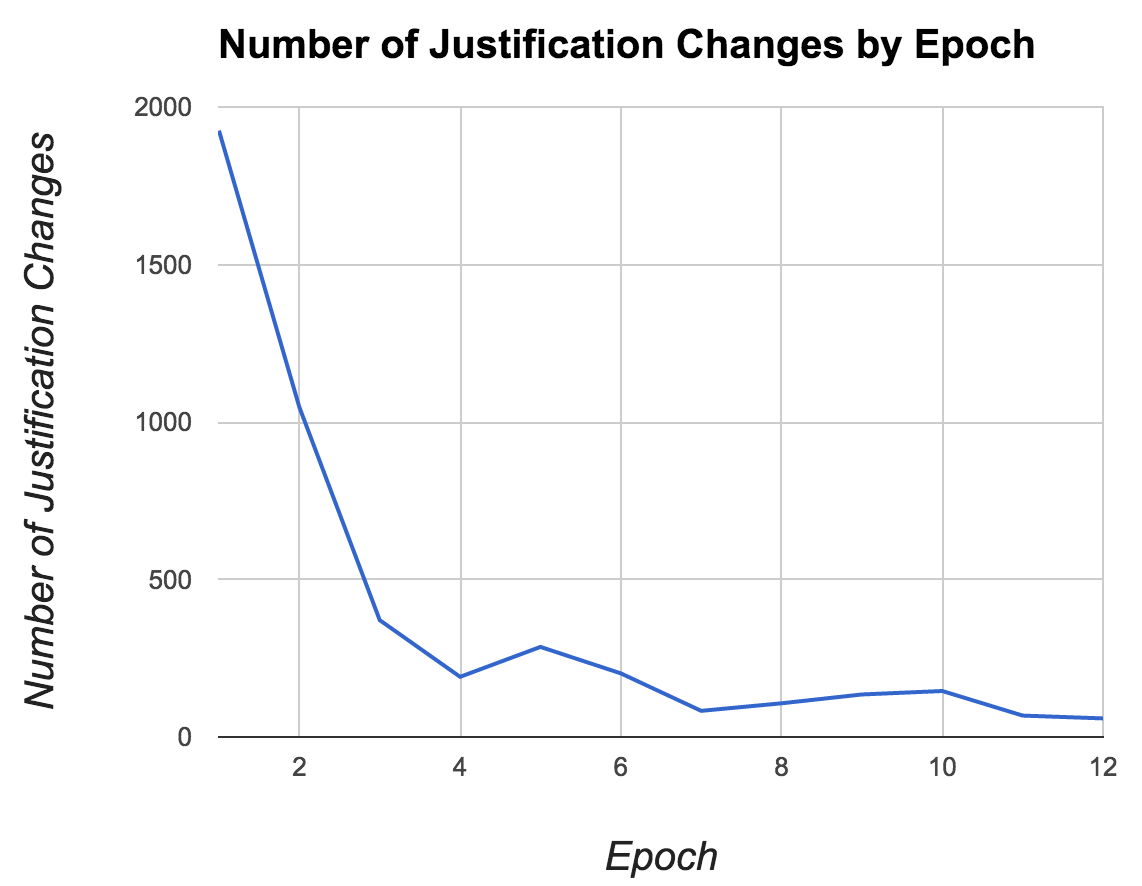
\includegraphics[width=0.7\textwidth]{mainmatter/emnlp2017-qaj/justificationChanges.png}
\caption{Number of questions for which % the IR$^{++}$ + EF + lexDisc + Emb 
our complete model chooses a new justification at each epoch during training.  While this is for a single random seed, we see essentially identical graphs for each random initialization.}
\label{fig:changes}
%space{-5mm}
\end{center}
\end{figure}

%\subsection{Contribution of Jointly Learning to Rank Justifications}
%\begin{flushleft}
%{\bf Contribution of Learning to Rerank Justifications}
%\end{flushleft}
%space{-2mm}
\paragraph{Contribution of Learning to Rerank Justifications:}
The main assertion of this work is that through learning to rank answers and justifications for those answer candidates in an end-to-end manner, we both answer questions correctly and provide justifications as to why the answer is correct.  To confirm that this is the case, we also ran a version of our system that does not re-rank justifications, but uses the top-ranked justification retrieved by IR.  This configuration dropped our performance on test to 48.7\% P@1, a decrease of 4.6\%, and we additionally lose all justification improvements from our system (see Section \ref{sec-emnlp2017:justification_results}), demonstrating that learning this reranking is key to our approach.

Additionally, we tracked the number of times a new justification was chosen by the model as it trained. We found that our system converges to a stable set of justifications during training, shown in Figure \ref{fig:changes}.



\begin{table}[t]
\begin{center}
\begin{tabular}{ll}
\hline
Error Type & Percent \\ 
\hline
Short justification/High lexical overlap  & 53.3\%\\
Complex inference required   & 43.3\% \\
Knowledge Base Noise  & 6.7\% \\
Word order necessary	 & 6.7\% \\
Coverage & 6.7\% \\
Negation	& 3.3\% \\
Other & 6.7\% \\
\end{tabular}

\caption{{ Summary of the findings of the 30 question error analysis.  
Examples of several categories are provided in separate tables. 
Note that a given question may fall into more than one category.}} 
\label{tab:erroranalysis}
\vspace{-5mm}
\end{center}
\end{table}

%\begin{table}[!th]
%\begin{center}
%\begin{footnotesize}
%\hfill
%\begin{tabular}{p{0.8cm}p{6.5cm}p{1cm}}
%\hline
%\multicolumn{2}{l}{Error Type} & Percent \\ 
%\hline
%\multicolumn{2}{l}{\textbf{Shorter justification with lots of lexical overlap}} & 53.3\%\\
%\multicolumn{2}{l}{\textbf{Complex inference required}}  & 43.3\% \\
%\hline
%
%\\
%\hline
%\multicolumn{2}{l}{\textbf{KB Noise}}  & 6.7\% \\
%\hline
%Question: & \multicolumn{2}{p{7.5cm}}{ If an object traveling to the right is acted upon by an unbalanced force from behind it  the object will}	\\
%Correct: & \multicolumn{2}{p{7.5cm}}{speed up }	\\
%Chosen & \multicolumn{2}{p{7.5cm}}{ change direction }	\\
%			& \multicolumn{2}{p{7.5cm}}{\textit{ Unbalanced force: force that acts on an object that will change its direction}}	\\
%%\hline
%\multicolumn{3}{p{8cm}}{The system found a sentence in the knowledge base that "justifies" the correct answer.}	\\
%%
%\\
%\hline
%\multicolumn{2}{l}{\textbf{Word order necessary}}	 & 6.7\% \\
%\hline
%Question: & \multicolumn{2}{p{7.5cm}}{ The acceleration of a small rocket that has just been launched can be quantitatively found by}	\\
%Correct: & \multicolumn{2}{p{7.5cm}}{dividing the force acting upon the rocket by its mass }	\\
%Chosen & \multicolumn{2}{p{7.5cm}}{ dividing the mass of the rocket by the force acting upon it }	\\
%			& \multicolumn{2}{p{7.5cm}}{\textit{ (same for both) acceleration: force divided by mass}}	\\
%%\hline
%\multicolumn{3}{p{8cm}}{The ordering of the answer choice terms was necessary for answering the question.}	\\
%%
%\\
%\hline
%\multicolumn{2}{l}{\textbf{Coverage}} & 6.7\% \\
%\hline
%Question: & \multicolumn{2}{p{7.5cm}}{ Which activity most effectively ensures the proper functioning of osteocytes?}	\\
%Correct: & \multicolumn{2}{p{7.5cm}}{consuming mineral-rich foods}\\
%			& \multicolumn{2}{p{7.5cm}}{\textit{ most lipids consumed from food are in the form of triglycerids}}	\\	
%Chosen & \multicolumn{2}{p{7.5cm}}{increasing the respiratory rate }	\\
%			& \multicolumn{2}{p{7.5cm}}{\textit{ hyperventilation increased respiratory rate}}	\\
%%\hline
%\multicolumn{3}{p{8cm}}{The knowledge base had no coverage for the concept of \emph{osteocyte}, so the system grasped at proverbial straws.}	\\
%%
%\\
%\hline
%\multicolumn{2}{l}{\textbf{Negation}}	& 3.3\% \\
%\hline
%%\multicolumn{3}{l}{Example}	\\
%Question: & \multicolumn{2}{p{7.5cm}}{ Which feature does not form as a result of tectonic plates diverging?}	\\
%Chosen: & \multicolumn{2}{p{7.5cm}}{ rift valley }	\\
%			& \multicolumn{2}{p{7.5cm}}{\textit{ Rift valley: deep valley formed as tectonic plates move apart. }}	\\
%\multicolumn{3}{p{8cm}}{Note that the justification actually shows that the chosen answer is incorrect, rather than justifying it.  This is the expected behavior for the system for these negated questions as we don't handle them differently.}	\\
%%
%\\
%\hline
%\multicolumn{2}{l}{\textbf{Other}} & 6.7\% \\
%\end{tabular}
%\hfill
%\end{footnotesize}
%\caption{{\footnotesize Summary of the findings of the 30 question error analysis.  Note that a given question may fall into more than one category.}} 
%\label{tab:erroranalysis}
%\end{center}
%\end{table}

\begin{table}[t]
\begin{center}
\begin{tabular}{p{2cm}p{12cm}}
\hline
Type: & \textbf{Short justification/High lexical overlap}\\
\hline
Question: & The length of time between night and day on Earth varies throughout the year. This time variance is explained primarily by $\rule{1cm}{0.15mm}$. \\
\\
Correct: & Earth 's angle of tilt \\
			 & \textit{ ... the days are very short in the winter because the sun's rays hit the earth at an extreme angle ... due to the tilt of the earth's axis. } \\
\\
Chosen: &  Earth 's distance from the Sun \\
			& \textit{ Is light year time or distance? Distance}	\\
\end{tabular}
\caption{{ Example of the system preferring a justification for which all the terms were found in either the question or answer candidate, while the justification for the correct answer contained additional information necessary to fully explain the answer. 
(Justifications shown in italics)
}} 
\label{tab:ex_lex_overlap}
\end{center}
\end{table}

\subsection{Error Analysis}
\label{sec-emnlp2017:erroranalysis}

To better understand the limitations of our current system, we performed an error analysis of 30 incorrectly answered questions.  
We examined the top 5 justifications returned for both the correct and chosen answers.  
Notably, 50\% of the questions analyzed had one or more good justifications in the top 5 returned by our system, but for a variety of reasons, summarized in Table \ref{tab:erroranalysis}, the system incorrectly ranked another justification higher.  

The table shows that the most common form of error was the system's apparent preference for short justifications with a large degree of lexical overlap with the question and answer choice itself, shown by the example in Table \ref{tab:ex_lex_overlap}.  The effect was magnified when the correct answer required more explanation to connect the question to the answer.  
This suggests that the system has learned that generally many unmatched words are indicative of an incorrect answer.  While this may typically be true, extending the system to be able to prefer the \emph{opposite} with certain types of questions would potentially help with these errors.  

\begin{table}[!th]
\begin{center}
\begin{tabular}{p{2cm}p{12cm}}
\hline
Type: & \textbf{Complex inference required}\\
\hline
Question: & Mr. Harris mows his lawn twice each month. He claims that it is better to leave the clippings on the ground. Which long term effect will this most likely have on his lawn? \\
\\
Correct: &  It will provide the lawn with needed nutrients. \\	
\end{tabular}
\caption{{ Example of a question for which complex inference is required.  In order to answer the question, you would need to assemble the event chain: cut grass left on the ground $\rightarrow$ grass decomposes $\rightarrow$ decomposed material provides nutrients.}} 
\label{tab:ex_complex_inf}
\end{center}
\end{table}

The second largest source of errors came from questions requiring complex inference (causal, process, quantitative, or model-based  reasoning) as with the question shown in Table \ref{tab:ex_complex_inf}.  This demonstrates not only the difficulty of the question set but also the need for systems that can robustly handle a variety of question types and their corresponding information needs.  


%The second largest source of errors came from questions requiring complex inference (causal, process, quantitative, or model-based  reasoning) as with the question:%.  For example, to answer the question:
 %\begin{quote}
%\begin{addmargin}[1em]{2em}% 1em left, 2em right 
% \begin{footnotesize}
%  \textit{Q: Mr. Harris mows his lawn ...[and leaves] the clippings on the ground. Which long term effect will this most likely have on his lawn? \\
%  A: It will provide the lawn with needed nutrients.}
% \end{footnotesize}
%%\end{quote}
%\end{addmargin}
%To answer this, you would need to link together: \textit{cut grass left on the ground $\rightarrow$ grass decomposes $\rightarrow$ decomposed material provides nutrients}. 
%These questions constitute a large portion of our errors,  
%is a large set of questions that our system is not particularly designed to handle, 
%demonstrating not only the difficulty of the question set but also the need for systems that can robustly handle a variety of question types and their corresponding information needs.  

\begin{table}[t]
\begin{center}
%\begin{footnotesize}
\begin{tabular}{p{2cm}p{12cm}}
\hline
Type: & \textbf{Knowledge base noise}\\
\hline
Question: & If an object traveling to the right is acted upon by an unbalanced force from behind it the object will $\rule{1cm}{0.15mm}$.\\
\\
Correct: & speed up\\
			%& \textit{Change of speed: an object accelerates if it speeds up and decelerates when it slows down}	\\	
\\
Chosen & change direction 	\\
			& \textit{ Unbalanced force: force that acts on an object that will change its direction}	\\
\end{tabular}
%\end{footnotesize}
\caption{{ Example of a question for which knowledge base noise (here, in the form of over-generalization) was an issue.}} 
\label{tab:ex_noise}
\end{center}
\end{table}


Aside from these primary sources of error, there were some smaller trends:  
7\% of the incorrectly chosen answers actually had justifications which ``validated'' them due to noise in the knowledge base (e.g., the example shown in Table \ref{tab:ex_noise}), 7\% required word-order to answer (e.g., \emph{mass divided by acceleration} vs. \emph{acceleration divided by mass}), another 7\% of questions suffered from lack of coverage of the question concept in the knowledge base,
%(see example in Table \ref{tab:ex_coverage}), 
 and 3\% failed to appropriately handle negation (i.e., questions of the format \emph{Which of the following are NOT ...}). 

%
%
%% bs: no room: - Negative results?


%\begin{table}[t]
%\begin{center}
%\begin{footnotesize}
%\begin{tabular}{p{1cm}p{6cm}}
%\hline
%Type: & \textbf{Coverage}\\
%\hline
%Question: & Which activity most effectively ensures the proper functioning of osteocytes? \\
%Correct: & consuming mineral-rich foods\\
%			& \textit{ most lipids consumed from food are in the form of triglycerids}	\\	
%Chosen & increasing the respiratory rate 	\\
%			& \textit{ hyperventilation increased respiratory rate}	\\
%\end{tabular}
%\hfill
%\end{footnotesize}
%\caption{{\footnotesize Example of a question for which coverage was an issue.  The KB had no coverage for the concept of \emph{osteocyte}.}} % , so the system grasped at proverbial straws.}} 
%\label{tab:ex_coverage}
%\end{center}
%\end{table}

 

%\begin{table}[!th]
%\begin{center}
%\begin{footnotesize}
%\hfill
%\begin{tabular}{ll}
%\hline
%Error Type & Percent \\ 
%\hline
%Short justification/High lexical overlap  & 53.3\%\\
%Complex inference required   & 43.3\% \\
%Knowledge Base Noise  & 6.7\% \\
%Word order necessary	 & 6.7\% \\
%Coverage & 6.7\% \\
%Negation	& 3.3\% \\
%Other & 6.7\% \\
%\end{tabular}
%\end{footnotesize}
%\caption{{\footnotesize Summary of the findings of the 30 question error analysis.  
%%Examples of several categories provided in separate tables. 
%Note that a given question may fall into more than one category.}} 
%\label{tab:erroranalysis}
%\vspace{-5mm}
%\end{center}
%\end{table}


%\begin{table}[t]
%\begin{center}
%\begin{footnotesize}
%\begin{tabular}{p{1cm}p{6cm}}
%\hline
%Type: & \textbf{Short justification/High lexical overlap}\\
%\hline
%Question: & The length of time between night and day on Earth varies throughout the year. This time variance is explained primarily by $\rule{1cm}{0.15mm}$. \\
%Correct: & Earth 's angle of tilt \\
%			 & \textit{ ... the days are very short in the winter because the sun's rays hit the earth at an extreme angle ... due to the tilt of the earth's axis. } \\
%Chosen: &  Earth 's distance from the Sun \\
%			& \textit{ Is light year time or distance? Distance}	\\
%\end{tabular}
%\hfill
%\end{footnotesize}
%\caption{{\footnotesize Example of the system preferring a justification for which all the terms were found in either the question or answer candidate. (Justifications shown in italics)
%}} 
%\label{tab:ex_lex_overlap}
%\vspace{-5mm}
%\end{center}
%\end{table}

\subsection{Error Analysis}
\label{sec-emnlp2017:erroranalysis}

We performed an error analysis of 30 incorrectly answered questions, %summarized in Table \ref{tab:erroranalysis},
  examining the top 5 justifications returned for both the correct and chosen answers of each.    
%Among the questions analyzed we found some interesting trends.   
Notably, 50\% of the questions had one or more \emph{Good} justifications. %, but the system incorrectly ranked another answer's justification higher.  
The most common form of error (53.3\%) was due to the system's preference for short justifications with a large degree of lexical overlap with the question and answer choice, %, particularly when the correct answer required more "explanation" to connect the question to the answer.  
% shown by the example in Table \ref{tab:ex_lex_overlap}.  
 %This effect was magnified when the correct answer required more "explanation" to connect the question to the answer.  
suggesting the system has learned that generally many unmatched words are indicative of an incorrect answer.  %While this may typically be true, extending the system to be able to prefer the \emph{opposite} with certain types of questions would potentially help with these errors.  
The second largest source of errors (43.3\%) came from questions requiring complex inference (causal, process, quantitative, or model-based reasoning), demonstrating the difficulty of the question set and the need for systems that can robustly handle a variety of question types.
Aside from these main groups, there were some smaller trends including KB noise, and our system's lack of using word order and recognizing negation.\footnote{A much more detailed error analysis is available, and if this paper is accepted will be included.}
 
% as with the question:%.  For example, to answer the question:
 %\begin{quote}
%\begin{addmargin}[1em]{2em}% 1em left, 2em right 
% \begin{footnotesize}
%  \textit{Q: Mr. Harris mows his lawn ...[and leaves] the clippings on the ground. Which long term effect will this most likely have on his lawn? \\
%  A: It will provide the lawn with needed nutrients.}
% \end{footnotesize}
%%\end{quote}
%\end{addmargin}
%To answer this, you would need to link together: \textit{cut grass left on the ground $\rightarrow$ grass decomposes $\rightarrow$ decomposed material provides nutrients}. 
%These questions constitute a large portion of our errors,   demonstrating not only the difficulty of the question set but also the need for systems that can robustly handle a variety of question types and their corresponding information needs.  

%Aside from these main groups, there were some smaller trends including:  
%7\% of the incorrectly chosen answers actually had justifications which "validated" them due to KB noise, 7\% required word-order to answer (e.g., \emph{X divided by Y} vs. \emph{Y divided by X}), %another 7\% of questions suffered from lack of coverage of the question concept in the knowledge base,
%%(see example in Table \ref{tab:ex_coverage}), 
% and 3\% failed to appropriately handle negation (i.e., questions of the format \emph{Which of the following are NOT ...}). 


% bs: no room: - Negative results?


%\begin{table}[t]
%\begin{center}
%\begin{footnotesize}
%\begin{tabular}{p{1cm}p{6cm}}
%\hline
%Type: & \textbf{Coverage}\\
%\hline
%Question: & Which activity most effectively ensures the proper functioning of osteocytes? \\
%Correct: & consuming mineral-rich foods\\
%			& \textit{ most lipids consumed from food are in the form of triglycerids}	\\	
%Chosen & increasing the respiratory rate 	\\
%			& \textit{ hyperventilation increased respiratory rate}	\\
%\end{tabular}
%\hfill
%\end{footnotesize}
%\caption{{\footnotesize Example of a question for which coverage was an issue.  The KB had no coverage for the concept of \emph{osteocyte}.}} % , so the system grasped at proverbial straws.}} 
%\label{tab:ex_coverage}
%\end{center}
%\end{table}


%\begin{table}[!th]
%\begin{center}
%\begin{footnotesize}
%\begin{tabular}{p{1cm}p{6cm}}
%\hline
%Type: & \textbf{Complex inference required}\\
%\hline
%Question: & Mr. Harris mows his lawn twice each month. He claims that it is better to leave the clippings on the ground. Which long term effect will this most likely have on his lawn? \\
%Correct: &  It will provide the lawn with needed nutrients. 	\\
%\end{tabular}
%\hfill
%\end{footnotesize}
%\caption{{\footnotesize Example of a question for which complex inference is required.  In order to answer the question, you would need to assemble the following chain of events: cut grass left on the ground $\rightarrow$ grass decomposes $\rightarrow$ decomposed material provides nutrients.}} 
%\label{tab:ex_complex_inf}
%\end{center}
%\end{table}


\section{Conclusion}
\label{sec-emnlp2017:conclusions}

Here we propose an end-to-end question answering (QA) model that learns to correctly answer questions as well as provide compelling, human-readable justifications for its answers,  despite not having access to labels for justification quality.  We do this by using the question answering task as a form of distant supervision for learning  justification re-ranking.  Similar in nature to the model proposed in Chapter \ref{chapter:cl2017}, we differ primarily in the shallower representation of our knowledge base texts (sentences versus graphlets) and the lack of aggregation in forming justifications.  These differences render this model more versatile -- they allow us to utilize larger corpora and consequently handle more challenging question sets that require more diverse background information to answer.   We show that our accuracy and justification quality are significantly better than a strong IR baseline, while maintaining near state-of-the-art performance for the answer selection task as well.  That is, without unduly sacrificing accuracy, with this approach we are able to provide explanations that complete the inference needed to connect questions and their answers.
%for selected answers that complete the inference to connect them to the corresponding questions.

Of the different types of features included in the model, we found that the explicit lexical overlap features were the most useful, and that the discourse and word embedding-based features each provided only a slight performance boost.  For the embedding-based features, this could be due to the limited amount of training data (often, neural networks that successfully learn feature representations operate over orders of magnitude more data than what we have available here).  Indeed, we found that when we attempted to update the word embeddings we ran into issues with  overfitting.  

Regarding the discourse features, with this approach we do not particularly address the different information needs of distinct question types (see \ref{sec:intro_emnlp2016}; cf., Chapter \ref{chapter:emnlp2016}), but intuitively different discourse relations may be more or less relevant to to each of them.  For example, a \textit{cause} relation may be more relevant to a causal question than it is to a definitional question.  Since our approach here does not allow for specialization of the model to different question types, this could be the reason for the underperformance of this discourse-based feature group.
%With this approach we do not particularly address the different information needs of distinct question types (see \ref{sec:intro_emnlp2016}; cf., Chapter \ref{chapter:emnlp2016}).  
Also, as discussed in the error analysis in Section \ref{sec-emnlp2017:erroranalysis}, of the incorrectly answered questions analyzed, 43.3\% required a form of complex inference such as \textit{causal} or \textit{quantitative} reasoning.  We hypothesize that by attempting to apply the same model to \textit{all} question types, we aren't able to specialize enough to handle these more complex information needs.   
While this framework can be extended to allow the model to learn different priorities for justification selection given different question information needs (perhaps similarly to the domain adaptation-based method that is used in Section \ref{sec-cl2017:characterizing}), we leave that extension to future work.  

Additionally, not performing aggregation to construct justifications constitutes a trade-off -- the approach is more lightweight (i.e., faster to run, and able to handle larger corpora within a given resource limit), but it becomes less likely that there exists a \textit{complete} justification for more complicated questions.  Likely there is a way to better balance the two -- perhaps by performing only selected aggregation during pre-processing, for topics that are more likely to need more than a single sentence to express.  Alternatively, perhaps reinforcement learning could be used to learn \textit{when} to add another sentence to an existing candidate justification for a given question and answer.  Again, we leave this exploration to future work.
%\FloatBarrier


%\section*{Acknowledgments}

%\bibliography{refs}
%\bibliographystyle{emnlp_natbib}
%
%\end{document}

\chapter{CONCLUSION\label{chapter:conclusion}}

%\address{briefly remind the reader of the big picture, what this work tells us generally}

In this work, we address the task of question answering (QA), \rev{which in simple terms comes down to querying a knowledge base, which could contain unstructured text or some structured information, to get a desired answer.  With this work we focus on knowledge bases composed of only unstructured text, the more common form of information available.}  Beyond the \rev{specific data} we use here, QA holds promise as a proving ground for developing tools and techniques to be able to navigate the vast sea of text knowledge that is now available, whose sheer size requires automated tools for usage.  

A successful QA approach must go beyond simple lexical lookup to perform inference -- anticipating the desired result based solely on the content of the question and the given background knowledge (i.e., the knowledge base).  As the majority of queries and knowledge base documents are written in natural language, this becomes a bit tougher --  
developing semantic representations of entire phrases or sentences is extremely difficult due to language variety, and yet when considered in isolation (i.e., a bag-of-words), some words are critical for the inference, some are distracting, and some lose much of their meaning without their context.  

Additionally, within a given question set there exists a wide range of question types with different forms of inference needed to solve them (i.e., different information needs).  Consider the difference between a question asking for an \textit{example} of a storm versus a question asking about the \textit{result} of a storm -- each requires a different form of inference to solve.  Consider also a question about the process by which a student might test the effect of sunlight on plants.  Unless there happens to be a single sentence explaining the entire process, many separate facts would need to be connected together to provide a complete explanation.  While this natural language inference is fairly trivial for a human to do, for an automated system it is very much a difficult, unsolved problem.

For QA methods which tackle the problem of natural language inference, we assert that to be truly useful, they must be \textbf{robust}, in that they should be able to handle a large range of questions with varied vocabulary and phrasing and they should be able to operate over large and diverse knowledge bases to allow for ample coverage.  Additionally, we suggest that these methods should be \textbf{interpretable}, or able to explain to a non-expert human user \textit{why} the selected answer was selected.  Without this ability, even when correct, users will hesitate to trust the output of the system.  When incorrect, interpretability is helpful too, as it gives insight into what changes need to be made in order to improve the performance.


Here we proposed a series of approaches that address these two desired attributes, robustness and interpretability, to varying degrees.  We began with a monolingual alignment approach in Chapter \ref{chapter:naacl2015} that we extended to be able to train over any free-text resource, rather than only over aligned question-answer pairs, by aligning the words associated with discourse relations found in the text (Section \ref{sec-naacl2015:approach}).  This makes this approach more robust than a traditional QA alignment model, as it extends the corpora over which it can operate, and we demonstrated its success in Section \ref{sec-naacl2015:results}.  This approach does not, however, address the different information needs present in a question set, rather it attempts to use the same set of learned word association scores for all words in all questions.  Following the intuition that certain discourse relations are better suited to certain information needs (e.g., the \textit{explanation} relation might be more relevant to \textit{Why} questions), this approach could be extended to see whether separate sets of alignments, each individualized to correspond to a single discourse relation, could be leveraged to address different types of questions.   While this is an investigation we leave to future work, we do propose a different approach that uses a model designed to address a specific relation.

In Chapter \ref{chapter:emnlp2016} we describe a framework for QA that would address different question information needs with different models, each tailored to a single need.  We train and evaluate a model for one of these needs, \textit{causality}.  Though we demonstrate that this relation-specific model is able to significantly improve upon a general-use model (Section \ref{sec-emnlp2016:results}), in terms of extending this method for use with a variety of questions, we do not particularly address the open-ended issue of determining \textit{what} relations would need to be handled.  Determining the needed relations by examining a given question set would guarantee some degree of relevancy, but it inherently adds bias and may limit the ability to generalize to unseen questions.  In practice, however, this may be the best way to proceed.  Even once a working set of relations is identified, classifying questions for which relation is appropriate would also be necessary and non-trivial, as the expense of manual labels would require using machine learning to train a classifier.
  
Additionally, while it was fairly straightforward to find cause-effect pairs to train the model (since causal language is often fairly explicit, as with phrases such as \textit{X led to Y} or \textit{Y was the result of X}), finding training data for many other relations may be trickier.  This suggests that extracted data for other relations my be noisier than what we extracted here for causality, which was itself a bit noisy.  While we proposed a simple method for mitigating noise, we hypothesize that improving the way that noise is handled would be very beneficial to any system that extends this approach to operate over more relations.

We also include two approaches that emphasize model interpretability.  For each of these we learn how to select both an answer to a question and a human-readable justification for why the answer is correct.  As we have no labeled training data for justifications, we use the model's performance in the QA task as supervision for both answer and justification selection.  That is, we score all potential justifications for each answer candidate and use the highest scoring as the current justification.  We use the intuition that the best justification for the correct answer should be better than the best justification for the other, incorrect answers (that is, the correct answer should be better supported by the knowledge base than the incorrect answers).  Thus, features from these top-scoring justifications are used to then rank the answer candidates themselves and update the model.  We use this basic framework to rerank answers and learn to select justifications in each of our latter two approaches, detailed in Chapters \ref{chapter:cl2017} and \ref{chapter:emnlp2017}, and in each we demonstrate that the justifications selected are better than those returned by a strong information retrieval baseline, as rated by humans. 
 
In Chapter \ref{chapter:cl2017}, we make use of a directed graph representation of knowledge base sentences based on a simplification of the sentence syntax, then aggregate multiple sentences together.  On the other hand, in Chapter \ref{chapter:emnlp2017} we use only single sentences for our justifications and we use deep learning to learn vector representations of our questions, answers, and justifications.  As a result, with the first approach we are able to use finer-grained features that make use of the structure of the justification graphs themselves, as well as features that characterize the lexical overlap between the aggregated sentences.   In the second approach, our features are coarser -- based only on the surface forms of the sentences (the sequence of words) and the representations learned over them.  However, the shallower representation of the knowledge base sentences means faster processing, which in practice allows for usage over the larger text resources which are arguably necessary for the more complicated questions we handle in Chapter \ref{chapter:emnlp2017} (8th grade versus 3rd-5th grade).        


Each of the models we propose in this work utilizes a bag-of-words approach.
%the discourse-based alignment model and the relation-specific lexical semantic model, 
As mentioned above, often the context of a word is necessary to determine the intended meaning, and many times word order is critical.  For example, consider the difference between a question asking for the state change of \textit{solid to liquid} versus \textit{liquid to solid}.  We are currently unable to handle these questions, though we hope to explore methods that go beyond bag-of-words to robustly handle phrases, sentences, and perhaps even paragraphs to handle arbitrarily more complex questions as well as larger answer and justification texts. 
Much work has been done on determining how to represent longer spans of text, \citep[inter alia,][]{Le2014DistributedRO, Sutskever2014SequenceTS, Pagliardini2017UnsupervisedLO}, but many of the popular techniques (including using Long-Short Term Memory Networks \citep[LSTMs;][]{hochreiter1997long}) require a very large amount of training data and struggle to generalize when presented infrequent or unseen vocabulary and phrasing.  Future work will explore available options for text representation, and perhaps explore new methods.  We hope to also explore deep learning as a means for learning (a) fixed-length representations of the graphlet structures described in Section \ref{sec-cl2017:tag} \citep{jansen2017framing}, and then hopefully (b) alignments between a graphlet representation of questions and answers and the graphlets from potential knowledge base sentence justifications.


While we have proposed several methods to address natural language inference for QA, there is still much to be done for this unsolved problem.  In these methods described here, as well as those we develop in the future, we plan to continue to invest in models which are robust to question variety, so as to maximize the utility of the model, and which are interpretable, and thus able to encourage confidence in the model predictions through providing a human-readable explanation by which a user can evaluate the provided answer.


%\address{summarize everything, don't necessarily repeat what you already said}


%\address{lay out where you’d go next to fill in or extend stuff}

%\address{Say what you learned + what are next steps (for the next student working on this)} 
%% Include the various appendices
%\appendix
\chapter{Causal Extraction Rules Appendix \label{appendix:rules}}

The ODIN \citep{valenzuela2016runes} taxonomy and rules used by the approach described in Section \ref{sec-emnlp2016:causalextraction}.  

\begin{singlespace}
\begin{small}

%\begin{lstlisting}
\begin{lstlisting}[label = {lst:tax}, caption = {ODIN taxonomy which provides the hierarchy of extracted entities and events.}]
  taxonomy:
  - Entity:
    - TransparentChunk
    - NP
    - CM:
      - CM_NP
      - CM_event
    - VP
    - Predicate
  - Event:
    - Causal
\end{lstlisting}


\begin{lstlisting}[label={lst:gramm_rules},
caption={Rules for grammatical primatives (e.g. noun phrases, prepositional phrases, etc).  These are used in a later step for finding the causal mentions.}]

  - name: entity_rule
    label: Entity
    priority: 1
    type: token
    pattern: |
      [word=/.+/]

  - name: np_rule_2
    label: NP
    priority: 2
    type: token
    unit: "tag"
    pattern: |
      /^NN/

  - name: vp_rule_1
    label: VP
    priority: 2
    type: token
    unit: "tag"
    pattern: |
      /^VB/
\end{lstlisting}

\begin{lstlisting}[caption={Rules for extracting causal mentions (CMs), which are the potential arguments for causal events.}]
  - name: CM_expansion
    label: CM_event
    priority: 4
    pattern: |
      trigger = [mention=VP & !lemma=/(cause|result|lead|create)/]
      deps:Entity* = /^(nsubj|nn|amod|advmod|ccmod|prep_(with|for|into|on|to)|dobj|xcomp|ccomp|agent|vmod)/{1,3}    


  - name: CM_expansion_2
    label: CM_NP
    priority: 3
    pattern: |
      trigger = [mention=NP & !lemma=/(cause|result)/]
      deps:Entity* = /^(nn|amod|advmod|ccmod|prep_(of|with|for|into|on|to|in)|dobj)/{1,3}   

  - name: CM_expansion_3_copular
    label: CM_event
    priority: 3
    pattern: |
      trigger = [lemma=be]
      deps:Entity* = /^(nsubj|prep_(in|on|with|for|of)|dobj|nn|amod)/+ 


  - name: nounphrase_with_property_3
    label: CM_NP
    priority: 5
    example: "... will cause huge <np> damage to the reef <\np>."
    pattern: |
      trigger = [mention=CM & !lemma=/(cause|result|lead|create)/]
      modifier:CM = <dobj [lemma=cause & tag=/^VB/] >/(prep_(to|for|of))|xcomp/
\end{lstlisting}

\begin{lstlisting}[caption={Rules for causal relations (events).  Note that the cause and effect arguments are previously found causal mentions.}] 

 - name: PosReg_syntax_1_verb
    label: Causal    
    priority: 9
    example: ""
    pattern: |
      trigger = [lemma=cause]
      controlled:CM+ = prepc_by? (dobj | xcomp | ccomp) 
      controller:CM+ = <xcomp? (nsubj | agent | <vmod) /appos|nn|conj_|cc|prep_of|prep_in/{,2}

  - name: causal_2
    label: Causal
    priority: 9
    example: "X will cause huge <np> damage to the reef <\np>."
    pattern: |
      trigger = [lemma=cause & tag=/^VB/]
      controlled:CM+ = dobj 
      controller:CM+ = nsubj

  - name: causal_3
    label: Causal
    priority: 9
    example: "X cause Y to Z"
    pattern: |
      trigger = [lemma=cause & tag=/^VB/]
      controlled:CM_event+ = xcomp 
      controller:CM+ = nsubj

  - name: causal_4
    label: Causal
    priority: 9
    example: "X was the cause of Y"
    pattern: |
      trigger = [lemma=cause & tag=/^NN/]
      controlled:CM+ = prep_of
      controller:CM+ = nsubj

  - name: causal_5
    label: Causal
    priority: 9
    example: "X was caused by Y"
    pattern: |
      trigger = [lemma=cause & tag=/^VB/]
      controlled:CM+ = nsubjpass
      controller:CM+ = agent

  - name: causal_6
    label: Causal
    priority: 9
    example: "They did not provide a motive for the alleged crime , which caused the city 's first fire-related deaths in more than a decade ."
    pattern: |
      trigger = [lemma=cause & tag=/^VB/]
      controlled:CM_NP = <rcmod (?= >rcmod >nsubj [tag=WDT])
      controller:CM+ = dobj

  - name: causal_7
    label: Causal
    priority: 9
    example: "After the exam grades begin to count , students often start taking them more seriously , which causes passage rates to increase , Jennings said ."
    pattern: |
      trigger = [lemma=cause & tag=/^VB/]
      controlled:CM_NP = <advcl (?= >advcl >nsubj [tag=WDT])
      controller:CM+ = dobj


  - name: result_1
    label: Causal
    priority: 9
    example: "X resulted in Y"
    pattern: |
      trigger = [lemma=result & tag=/^VB/]
      controlled:CM+ = prep_in
      controller:CM+ = nsubj

  - name: result_2
    label: Causal
    priority: 9
    example: "X as a result of Y"
    pattern: |
      trigger = [lemma=result & tag=/^NN/]
      controlled:CM+ = <prep_as
      controller:CM+ = prep_of

  - name: result_3
    label: Causal
    priority: 9
    example: "X was the result of Y"
    pattern: |
      trigger = [lemma=result & tag=/^NN/]
      controlled:CM+ = nsubj
      controller:CM+ = prep_of

  - name: result_4
    label: Causal
    priority: 9
    example: "Jet lag results when the body 's internal clock is out of sync with daily life , making people sleepy when they want to be awake and wakeful when they want to sleep."
    pattern: |
      trigger = [lemma=result & tag=/^VB/]
      controlled:CM+ = nsubj
      controller:CM+ = /(advcl|prep_from)/

  - name: led_to_1
    label: Causal
    priority: 9
    example: "X led to Y"
    pattern: |
      trigger = [lemma=lead & tag=/^(VB|NN)/] to
      controller:CM+ = nsubj
      controlled:CM+ = prep_to

  - name: create_1
    label: Causal
    priority: 9
    example: "X was created by Y"
    pattern: |
      trigger = [lemma=create & tag=/^VB/]  
      controlled:CM+ = nsubjpass
      controller:CM+ = agent

\end{lstlisting}
\end{small}
\end{singlespace}



% Switch the spacing to single-spaced for the references
\renewcommand{\baselinestretch}{1}		% changing the value
\small\normalsize										% switch size to make the value take

% Create the References list
\bibliographystyle{uabibnat}
\bibliography{mainmatter/refs}

\end{document}
